\documentclass{beamer}


\usepackage{beamerthemesplit}
\usepackage[utf8]{inputenc}
\usepackage[english]{babel}
\usepackage[T1]{fontenc}
%\usepackage{mathenv}
\usepackage{empheq}
%\usepackage{subfigure}
\usepackage{multimedia}
\usepackage{pgf,tikz}
\usetikzlibrary{positioning,arrows,shapes,snakes}
%\usepackage[pdftex]{hyperref}
\usepackage{mathrsfs}
\usepackage{mathtools}
\mathtoolsset{showonlyrefs=true}

\usepackage{multicol}
\usepackage{empheq}
\usepackage{textpos}
\usepackage{graphics}
% Or whatever. Note that the encoding and the font should match. If T1
% does not look nice, try deleting the line with the fontenc.
\usepackage{helvet}
\usepackage{tikz,pgfplots,xcolor}

%%%%%%% Packages et corrections ajoutés à la volée %%%%%%%%%%%%%
\usepackage{graphicx,multimedia}
\usepackage{xpatch}
\usepackage{fourier-orns}
\usepackage[style=verbose,backend=bibtex]{biblatex}
\usepackage{subcaption}
\addbibresource{zotero.bib}
\usepackage{amsmath}
\xpatchbibmacro{cite}{cite:short}{cite:full}{}{}
\usepackage{colortbl}
\renewcommand{\footnotesize}{\fontsize{7pt}{9pt}\selectfont}
\usetikzlibrary{patterns}
 \usetikzlibrary{arrows,automata,calc,shapes, positioning,shadows,shadows.blur,shapes.geometric}

 \definecolor{col2}{HTML}{a11919}%couleur des barres de l'histo


%========================================================================
%========================== BEAMER options ==============================
%========================================================================

\beamertemplateshadingbackground{blue!5}{structure!5}
\beamertemplatetransparentcovereddynamic
\beamertemplateballitem
\beamertemplatenumberedballsectiontoc

\title[Time-Domain FWI using advanced DG methods]{Time-Domain Full Waveform Inversion using advanced Galerkin Discontinuous methods}
%\title{Petit titre}
\author{Pierre Jacquet}
\institute{Université de Pau et des Pays de l'Adour \\
  INRIA Bordeaux Sud-Ouest, Project-Team Magique 3D \\
Laboratory of Mathematics and its Applications of PAU}
\date{February 25, 2021}


%\setbeamertemplate{footline}[frame number]
\setbeamertemplate{page number in head/foot}{\insertframenumber}
\usetheme[secheader]{Madrid}


\usecolortheme{myblue}
\usecolortheme{beaver}
\definecolor{mainTitl2}{HTML}{a7a7a7}
\definecolor{mainTitl}{HTML}{dddddd}
\definecolor{mainRed}{HTML}{a11919}

\setbeamercolor*{palette tertiary}{bg=mainRed,fg=gray!10!white} % up 1 + down 1
\setbeamercolor*{palette primary}{fg=mainRed,bg=mainTitl2}  % up 2 + down 3
\setbeamercolor*{palette secondary}{fg=mainRed,bg=mainTitl} % down 2
\setbeamercolor{frametitle}{bg=mainTitl,fg=mainRed}
\setbeamercolor{block title}{bg=mainRed, fg=white}
\setbeamercolor{titlelike}{parent=palette tertiary,fg=white} %Main titile

%% \definecolor{myNewColorA}{rgb}{0.85,0.07,0.07}
%% \definecolor{myNewColorB}{rgb}{0.1, 0.9, 0.3}
%% \definecolor{myNewColorC}{rgb}{0.1, 0.9, 0.9}
%% \definecolor{myNewColorD}{rgb}{0.1, 0.1, 0.3}

%%  %% \setbeamercolor*{palette primary}{bg=myNewColorA, fg = white}
%%  %%  \setbeamercolor*{palette secondary}{bg=myNewColorB, fg = white}
%%   \setbeamercolor*{palette tertiary}{bg=myNewColorC, fg = white}
%%   \setbeamercolor*{palette quaternary}{bg=myNewColorD, fg = white}

 \beamertemplatenavigationsymbolsempty


\makeatletter
\setbeamertemplate{footline}
{
  \leavevmode%
  \hbox{%
  \begin{beamercolorbox}[wd=.2\paperwidth,ht=2.25ex,dp=1ex,center]{author in head/foot}%
    \usebeamerfont{author in head/foot}\insertshortauthor%~~\beamer@ifempty{\insertshortinstitute}{}{(\insertshortinstitute)}
  \end{beamercolorbox}%
  \begin{beamercolorbox}[wd=.5\paperwidth,ht=2.25ex,dp=1ex,center]{title in head/foot}%
    \usebeamerfont{title in head/foot}\insertshorttitle
  \end{beamercolorbox}%
  \begin{beamercolorbox}[wd=.3\paperwidth,ht=2.25ex,dp=1ex,right]{date in head/foot}%
    \usebeamerfont{date in head/foot}\insertshortdate{}\hspace*{2em}
    \insertframenumber{} / \inserttotalframenumber\hspace*{2ex}
  \end{beamercolorbox}}%
  \vskip0pt%
}
\makeatother

%========================================================================
%========================================================================
%========================================================================


%========================================================================
%==================== PAGE DE GARDE =====================================
%========================================================================


\makeatletter
\newcommand\titlegraphicii[1]{\def\inserttitlegraphicii{#1}}
\centering
\titlegraphicii{}
\setbeamertemplate{title page}
{
  \vbox{}
   {\usebeamercolor[fg]{titlegraphic}\inserttitlegraphic\hfill\inserttitlegraphicii\par}
  \begin{centering}
    \begin{beamercolorbox}[sep=8pt,center]{institute}
      \usebeamerfont{institute}\insertinstitute
    \end{beamercolorbox}
    \begin{beamercolorbox}[sep=8pt,center]{title}
      \usebeamerfont{title}\inserttitle\par%
      \ifx\insertsubtitle\@empty%
      \else%
        \vskip0.25em%
        {\usebeamerfont{subtitle}\usebeamercolor[fg]{subtitle}\insertsubtitle\par}%
      \fi%
    \end{beamercolorbox}%
    \vskip1em\par
    \begin{beamercolorbox}[sep=8pt,center]{date}
      \usebeamerfont{date}\insertdate
    \end{beamercolorbox}%\vskip0.5em
    \begin{beamercolorbox}[sep=8pt,center]{author}
      \usebeamerfont{author}\insertauthor
    \end{beamercolorbox}
  \end{centering}
  %\vfill
}
\makeatother
\author{\textbf{Pierre Jacquet}}
\title[Time-Domain FWI using advanced DG methods]{Time-Domain Full Waveform Inversion using advanced Discontinuous Galerkin methods}
\institute{Université de Pau et des Pays de l'Adour \\
  INRIA Bordeaux Sud-Ouest, Project-Team Magique 3D \\
Laboratory of Mathematics and its Applications of Pau}
\date{February 25, 2021}
  \titlegraphic{
\includegraphics[scale=0.25]{inria2}}

%========================================================================
%========================================================================
%========================================================================



\pgfplotsset{compat=newest}

%%%%%% TIKZ SET STYLE %%%%%%%%
\tikzset{boxOptions/.style={
    rectangle,
    rounded corners,
    draw=black, very thick,
    text width=9em,
    minimum height=2em,
    text centered}
}

\tikzset{arrowStyle/.style={
    ->,
    thick,
    shorten <=2pt,
    shorten >=2pt}
}

\tikzset{arrowStyleinv/.style={
    <-,
    thick,
    shorten <=2pt,
    shorten >=2pt}
}

\usetikzlibrary{backgrounds}

\newcommand\tikzscale{0cm}
\newlength{\tikzwidth}
\newlength{\tikzheight}

%%%%%%%%%%%%%%%%%%%%%%%%%%%%

% colored hyperlinks
\newcommand{\chref}[2]{%
  \href{#1}{{\usebeamercolor[bg]{AAUsimple}#2}}%
}
\newcommand{\scaption}[1]{\caption{\tiny{#1}}}


\definecolor{light-gray}{gray}{0.95}
\definecolor{myred}{RGB}{200,0,0}
\newcommand{\myred}{red!70!black}
\newcommand{\mygreen}{green!60!black}
\newcommand{\myblue}{blue!40!black}
\newcommand{\code}[1]{\colorbox{light-gray}{\texttt{#1}}}


\newcommand\discreteP{\boldsymbol{\textcolor{\myred}{\bar{P}}}}
\newcommand\discreteV{\boldsymbol{\textcolor{\myred}{\bar{V}}}}
\newcommand\discreteU{\boldsymbol{\textcolor{\myred}{\bar{U}}}}
\newcommand\discreteF{\boldsymbol{\bar{F}}}
\newcommand\discreteG{\boldsymbol{\bar{G}}}

\newcommand\discreteQP{\bar{q_p}}
\newcommand\discreteQV{\bar{q_v}}
\newcommand\discreteQ{\bar{q}}
%\newcommand\discreteD{\bar{d}}
%\newcommand\Lag{\boldsymbol{\mathcal{L}}}


\newcommand\qcqU{\textcolor{\myred}{\widehat{\boldsymbol{{u}}}}}
\newcommand\qcqP{\widehat{p}}
\newcommand\qcqV{\widehat{\textbf{v}}}
\newcommand\contLbd{\boldsymbol{\textcolor{\myblue}{\lambda}}}
\newcommand\qcqLbd{\boldsymbol{\textcolor{\myblue}{\widehat{\lambda}}}}
\newcommand\Lbdun{\boldsymbol{\textcolor{\myred}{\lambda_1}}}
\newcommand\Lbdeux{\boldsymbol{\textcolor{\myred}{\lambda_2}}}
\newcommand\qcqLbdun{\widehat{\lambda_1}}
\newcommand\qcqLbdeux{\boldsymbol{\widehat{\lambda_2}}}

\newcommand\discreteLbd{\textcolor{\myred}{\boldsymbol{\bar{\Lambda}}}}
\newcommand\discreteLbdun{\textcolor{\myred}{\boldsymbol{\bar{\Lambda_1}}}}
\newcommand\discreteLbdeux{\textcolor{\myred}{\boldsymbol{\bar{\Lambda_2}}}}
\newcommand\discreteD{\boldsymbol{\bar{D}}}

%\newcommand\CF{\mathcal{J}}
\newcommand\CFF{\mathcal{G}}
\newcommand\DP{Forward_{\model}}

\newcommand\contAl{\boldsymbol{\alpha}}

%% \newcommand\velocity{v_p}
%% \newcommand\density{\rho_0}
%\newcommand\velocity{\boldsymbol{\textcolor{\mygreen}{c}}}
\newcommand\bulkmodulus{\boldsymbol{\textcolor{\mygreen}{\kappa}}}
%\newcommand\density{\boldsymbol{\textcolor{\mygreen}{\rho}}}


\pgfplotsset{
        colormap/paraview/.style={
                colormap={paraview}{
                        rgb255(0cm)=(20,119,255)
			rgb255(1cm)=(168,181,255)
			rgb255(2cm)=(240,240,240)
			rgb255(3cm)=(255,161,145)
                        rgb255(4cm)=(234,60,53)
                },
        },
}


\newcommand\vectll[4]{\left#1 \begin{array}{c}
    #2\\
    #3\\
  \end{array} \right#4}

%%%%% SETUP %%%%%

\newcommand{\cmark}{\ding{51}}%
\newcommand{\xmark}{\ding{55}}%
\newcommand{\greencheck}{{\textcolor{\mygreen}{\cmark}}}
\newcommand{\redcross}{{\textcolor{red}{\xmark}}}

\newcommand{\fig}[1]{Figure~\ref{#1}}
\newcommand{\tab}[1]{Table~\ref{#1}}
\newcommand{\jd}[1]{\textbf{\textcolor{magenta}{#1}}}
\newcommand{\hb}[1]{\textbf{\textcolor{purple!95!black}{#1}}}
\newcommand{\pj}[1]{\textbf{\textcolor{green!95!black}{#1}}}

\newcommand{\jump}[1]{\llbracket#1\rrbracket}
\newcommand{\average}[1]{\{#1\}}

%%%% BB %%%%
\newcommand{\lzero}{{\hat{\lambda_0}}}
\newcommand{\lone}{{\hat{\lambda_1}}}
\newcommand{\ltwo}{{\hat{\lambda_2}}}
\newcommand{\lthree}{{\hat{\lambda_3}}}
\newcommand{\lfour}{{\hat{\lambda_4}}}

\newcommand{\balpha}{{\boldsymbol{\alpha}}}
\newcommand{\bbeta}{{\boldsymbol{\beta}}}
\newcommand{\blambda}{{\boldsymbol{\hat{\lambda}}}}

\newcommand{\bgamma}{{\boldsymbol{\gamma}}}
\newcommand{\bdelta}{{\boldsymbol{\delta}}}

\newcommand{\Lift}{{L}}

%%%%% WADG %%%%%%%%%%%%%%%%

\newcommand{\param}{{\gamma}}
\newcommand{\coefParam}{{\boldsymbol{\gamma}}}
\newcommand{\weight}{{\boldsymbol{\hat{\omega}}}}
\newcommand{\sweight}{{\hat{\omega}}}
\newcommand{\Mwadg}{{\overset{\sim}{{M}}}}
\newcommand{\nquad}{{n_q}}

\newcommand{\Pquad}{{\bar{Q}}}
\newcommand{\QuadOrder}{{N_q}}


%%%% ENVIRONNEMENT %%%%%



%% \mdfsetup{skipabove=\topskip,skipbelow=\topskip}
%% \tikzset{titre_industry/.style =
%% 	{draw=black, line width=1.5pt, fill=gray!5,
%% 	rectangle, rounded corners, right,minimum height=2em}}
%% \newcommand{\titreencadre}{Titre}
%% \makeatletter
%% \mdfdefinestyle{encadrestyle}{%
%% 	linewidth=1.5pt,roundcorner=5pt,linecolor=black,
%% 	apptotikzsetting={\tikzset{mdfbackground/.append style ={%
%% 		fill=gray!15}}},
%% 	frametitlefont=\bfseries,
%% 	singleextra={%
%% 		\node[titre_industry,xshift=2em] at (P-|O) %
%% 			{~\mdf@frametitlefont{\titreencadre}\hbox{~}};},
%% 	firstextra={%
%% 		\node[titre_industry,xshift=2em] at (P-|O) %
%% 		{~\mdf@frametitlefont{\titreencadre}\hbox{~}};},
%% 	}
%% \mdfdefinestyle{encadresanstitrestyle}{%
%% 	linewidth=1.5pt,roundcorner=5pt,linecolor=orange,
%% 	apptotikzsetting={\tikzset{mdfbackground/.append style ={%
%% 		fill=yellow!20}}},
%% }

%% \newenvironment{industry}{\renewcommand{\titreencadre}{Industrial context}
%% 	\begin{mdframed}[style=encadrestyle]
%% 	\vspace{0.8\baselineskip}
%% 	}{%
%% \end{mdframed}}

%% \newenvironment{p_note}{\renewcommand{\titreencadre}{Personal note}
%% 	\begin{mdframed}[style=encadrestyle]
%% 	\vspace{0.8\baselineskip}
%% 	}{%
%% 	\end{mdframed}}



\newenvironment{conditions}
{\par\vspace{\abovedisplayskip}\noindent\begin{tabular}{>{$}l<{$} @{${}={}$} l}}
{\end{tabular}\par\vspace{\belowdisplayskip}}


\newcommand{\cmapmin}{0}
\newcommand{\cmapmax}{1}

\newcommand{\modelfile}{default}


%%%%% SIZE %%%%%%%

\newlength{\plotwidth}
\newlength{\plotheight}


\newlength{\modelwidth}


%%%%%% PROTOCOL EXP %%%%%%%%%%%

\newcommand\tpeak{{t_{peak}}}
\newcommand\fpeak{{f_{peak}}}
\newcommand\fmax{{f_{max}}}


%%%%%% MACRO %%%%%%%%%%%.

\newcommand\dangersign[1][2ex]{%
  \renewcommand\stacktype{L}%
  \scaleto{\stackon[1.3pt]{\color{red}$\triangle$}{\tiny\bfseries !}}{#1}}



%%% Inconnu probleme direct
\newcommand\dt{\partial t}

\newcommand\x{{\boldsymbol{x}}}
\newcommand\xx{{x_1}}
\newcommand\xy{{x_2}}
\newcommand\xz{{x_3}}
\newcommand\xd{{x_d}}


\newcommand\colorcontP{\boldsymbol{\textcolor{\myred}{p}}}
\newcommand\colorcontV{\boldsymbol{\textcolor{\myred}{v}}}


%\newcommand\adjP{{\lambda_p}}
\newcommand\adjP{{\contP^*}}
\newcommand\PolAdjP{{(\contP^*)_h}}
\newcommand\CoefPolAdjP{{(P^*)_h}}

%% \newcommand\adjV{{\boldsymbol{\lambda_v}}}
%% \newcommand\adjVd{{\lambda_{v_d}}}
\newcommand\adjV{{\boldsymbol{\contV^*}}}
\newcommand\adjVd{{\contVd^*}}
\newcommand\PolAdjV{{(\adjV)_h}}

\newcommand\scoefAdjP{{(P^*)_h}}
\newcommand\coefAdjP{{\boldsymbol{\scoefAdjP}}}
\newcommand\coefAdjPj{{\scoefAdjP_{j}}}

\newcommand\scoefAdjV{{(V^*)_h}}
\newcommand\coefAdjVd{{\scoefAdjV_{d}}}
\newcommand\scoefAdjVd{{\scoefAdjV_{d}}}
\newcommand\coefAdjVdj{{\scoefAdjV_{d_j}}}
\newcommand\coefAdjV{{\boldsymbol{\scoefAdjV}}}
\newcommand\coefAdjVj{{\scoefAdjP_{j}}}


\newcommand\contP{{\textcolor{\myred}{p}}}
\newcommand\dtcontP{{\frac{\partial \contP}{\dt}}}

\newcommand\contV{\boldsymbol{\textcolor{\myred}{v}}}
\newcommand\contVx{{v_{\xx}}}
\newcommand\contVy{{v_\xy}}
\newcommand\contVz{{v_\xz}}
\newcommand\contVd{{v_d}}

\newcommand\contU{{\boldsymbol{\textcolor{\myred}{u}}}}
\newcommand\adjU{{\boldsymbol{{\lambda}}}}


\newcommand{\fracdt}{{ \frac{\partial}{\partial t}}}
\newcommand{\fracdx}{{ \frac{\partial}{\partial \xx}}}
\newcommand{\fracdy}{{ \frac{\partial}{\partial \xy}}}
\newcommand{\fracdz}{{ \frac{\partial}{\partial \xz}}}
\newcommand{\fracdd}{{ \frac{\partial}{\partial \xd}}}

\newcommand{\fracdrefx}{{ \frac{\partial}{\partial \refxx}}}
\newcommand{\fracdrefy}{{ \frac{\partial}{\partial \refxy}}}
\newcommand{\fracdrefz}{{ \frac{\partial}{\partial \refxz}}}
\newcommand{\fracdrefd}{{ \frac{\partial}{\partial \refxd}}}


\newcommand\dtcontV{{\frac{\partial \contV}{\dt}}}

\newcommand\polP{{p_h}}
\newcommand\scoefPolP{{P_h}}
\newcommand\coefPolP{{\boldsymbol{P_h}}}
\newcommand\coefPolPj{{P_{h_j}}}
\newcommand\sdtcoefPolP{{\frac{\partial P_h}{\partial t}}}
\newcommand\dtcoefPolP{{\frac{\partial \boldsymbol{P_h}}{\partial t}}}
\newcommand\dtcoefPolPj{{\frac{\partial P_{h_j}}{\partial t}}}
\newcommand\spolV{{v_h}}

\newcommand\polV{\boldsymbol{\spolV}}
\newcommand\polVx{{\spolV_1}}
\newcommand\polVy{{\spolV_2}}
\newcommand\polVz{{\spolV_3}}
\newcommand\polVd{{\spolV_d}}


\newcommand\scoefPolV{{V_h}}
\newcommand\coefPolV{{\boldsymbol{\scoefPolV}}}
\newcommand\coefPolVd{{\coefPolV_d}}
\newcommand\coefPolVdj{{\scoefPolV_{d_j}}}
\newcommand\scoefPolVd{{\scoefPolV_{d}}}
\newcommand\scoefPolVdj{{\scoefPolV_{d_j}}}
\newcommand\coefPolVj{{\coefPolV_{j}}}

\newcommand\dtcoefPolV{\frac{\partial \coefPolV}{\partial t}}
\newcommand\dtcoefPolVd{\frac{\partial \coefPolVd}{\partial t}}


\newcommand\UGlob{{\boldsymbol{U}}}
\newcommand\UGGlob{{\boldsymbol{\bar{U}}}}
\newcommand\FGlob{{\boldsymbol{F}}}
\newcommand\FGGlob{{\boldsymbol{\bar{F}}}}
\newcommand\AdjFGGlob{{\boldsymbol{\bar{G}}}}

\newcommand\AdjUGGlob{{\boldsymbol{\bar{\Lambda}}}}

\newcommand\coefpolSource{{\boldsymbol{F_h}}}
\newcommand\coefpolSourcej{{F_{h_j}}}

\newcommand\dtpolP{\frac{\partial \polP}{\dt}}
\newcommand\dtContP{\frac{\partial \contP}{\dt}}
\newcommand\dttContP{\frac{\partial^2 \contP}{\dt^2}}

\newcommand\dtpolV{{\frac{\partial \polV}{\dt}}}
\newcommand\dtpolVx{{\frac{\partial \polVx}{\dt}}}
\newcommand\dtpolVy{{\frac{\partial \polVy}{\dt}}}
\newcommand\dtpolVz{{\frac{\partial \polVz}{\dt}}}
\newcommand\dtpolVd{{\frac{\partial \polVd}{\dt}}}


\newcommand\sdtpolV{{\frac{\partial \spolV}{\dt}}}

\newcommand\testP{q}
\newcommand\stestV{w}
\newcommand\testV{\boldsymbol{\stestV}}
\newcommand\testVx{{\stestV_1}}
\newcommand\testVy{{\stestV_2}}
\newcommand\testVz{{\stestV_3}}
\newcommand\testVd{{\stestV_d}}

\newcommand\PolOrder{{N}}

\newcommand\SpacePolP{{\mathcal{Q}_h^\PolOrder}}
\newcommand\SpacePolV{{\boldsymbol{\mathcal{W}_h^\PolOrder}}}

\newcommand\SpaceTestP{{\mathcal{Q}}}
\newcommand\SpaceTestV{{\boldsymbol{\mathcal{W}}}}

\renewcommand\dim{{dim}}
\newcommand\dof{{DoF}}

\newcommand\elementK{{K}}
\newcommand\element{{K}}
\newcommand\refelement{{\hat{K}}}

\newcommand\refx{{\boldsymbol{\hat{x}}}}
\newcommand\refxx{{\hat{x_1}}}
\newcommand\refxy{{\hat{x_2}}}
\newcommand\refxz{{\hat{x_3}}}
\newcommand\refxd{{\hat{x_d}}}
\newcommand\ecan{{\boldsymbol{e}}}



\newcommand\nbelem{{N_e}}
\newcommand\Triangles{{\mathcal{T}_h}}
\newcommand\Domain{{\Omega}}
\newcommand\BDomain{{\partial \Omega}}
\newcommand\DomainInf{{\Omega_{inf}}}
\newcommand\normal{{\boldsymbol{n}}}
\newcommand\snormal{{n}}
\newcommand\Edge{{\Gamma}}

\newcommand{\Bext}{{\mathcal{B}_{ext}}}
\newcommand{\Bint}{{\mathcal{B}_{int}}}
\newcommand{\dk}{{d { \scriptstyle \element}}}
\newcommand{\drefk}{{d { \scriptstyle \hat{\element}}}}
\newcommand{\ds}{{d s}}
\newcommand{\drefs}{{d \hat{s}}}

%\newcommand\detJK{\mathcal{J}_\element}
%\newcommand\detJF{\mathcal{J}_\Gamma}
\newcommand\detJF{|T_\Gamma|}
\newcommand\detJK{|T_\element|}
\newcommand\detJKl{|T_{\element^l}|}


\newcommand\refphi{\hat{\varphi}}

\newcommand\Mass{{M}}
\newcommand\MassRef{{\hat{M}}}
\newcommand\MassGlob{{{M^{glob}}}}
\newcommand\MassGlobEdge{{{M_\Edge^{glob}}}}
\newcommand\Stiff{{S}}
\newcommand\StiffRef{{\hat{S}}}
\newcommand\StiffGlob{{S_d^{glob}}}
\newcommand\StiffGlobx{{S_x^{glob}}}
\newcommand\StiffGloby{{S_y^{glob}}}
\newcommand\StiffGlobz{{S_z^{glob}}}
\newcommand\Diff{{\hat{D}}}
\newcommand\Diffd{{\Diff_d}}
\newcommand\Diffx{{\Diff_\refxx}}
\newcommand\Diffy{{\Diff_\refxy}}
\newcommand\Diffz{{\Diff_\refxz}}

\newcommand\Difflzero{{\Diff_\lzero}}
\newcommand\Difflone{{\Diff_\lone}}
\newcommand\Diffltwo{{\Diff_\ltwo}}
\newcommand\Difflthree{{\Diff_\lthree}}

\newcommand\FluxP{{\mathcal{F}_p}}
\newcommand\FluxV{{\mathcal{F}_v}}

\newcommand\vFluxP{{\bar{\boldsymbol{\mathcal{F}_p}}}}
\newcommand\vFluxV{{\bar{\boldsymbol{\mathcal{F}_v}}}}

%%%%% Time scheme %%%%%

\newcommand\dx{{\Delta x}}
\newcommand\deltat{{\Delta t}}
\newcommand\h{{\Delta t}}
\newcommand\RHS{{\mathcal{L}}}

%%%%% INVERSE PROBLEM %%%%%%%%%%%%

\newcommand\smodel{{\textcolor{\mygreen}{m}}}
\newcommand\model{{\boldsymbol{\smodel}}}

\newcommand\contModel{{m}}

\newcommand\contWavefield{{u}}
\newcommand\contQcqWavefield{{\widehat{u}}}

\newcommand\contAdjoint{{\lambda}}
\newcommand\contQcqAdjoint{{\widehat{\lambda}}}


\newcommand\wavefield{{\boldsymbol{u}}}

\newcommand\WCF{{\mathcal{W}}_2}

\newcommand\CF{{\mathcal{J}}}

\newcommand\CFu{{\hat{\mathcal{J}}}}

\newcommand\gradCF{\nabla{\mathcal{J}}}

\newcommand\Restriction{{\mathcal{R}}}
\newcommand\Functional{{\mathcal{F}}}
\newcommand\data{{d}}
\newcommand\Tfinal{{T_f}}

\newcommand\Lagrangian{{\mathcal{L}}}
\newcommand\Lag{{\mathcal{L}}}

\newcommand\dobs{{d_{obs}}}
\newcommand\nrcv{{n_{rcv}}}
\newcommand\nsrc{{n_{src}}}
\newcommand\nsample{{n_t}}
\newcommand\nt{{N_t}}
\newcommand\dtsample{{dt}}

\newcommand\RestSpace{{\Restriction_x}}
\newcommand\RestTime{{\Restriction_t}}

\newcommand\nparam{{n_{p}}}



%%%%%%% OPTIM %%%%%%%%%%

\newcommand\SD{{d}}
\newcommand\LS{\alpha}

%\newcommand\dim{{dim}}


%%% parameters

\newcommand\density{\textcolor{\mygreen}{\rho}}
\newcommand\velocity{\textcolor{\mygreen}{c}}
\newcommand\bm{\textcolor{\mygreen}{\kappa}}


%%%%% MESH

\newcommand\nppw{n_{ppw}}
\newcommand\metric{\mathcal{M}}

%%%%%%%%% COLORMAP %%%%%%%%%%%%%

\pgfplotsset{
  colormap/paraview/.style={
    colormap={paraview}{
      rgb255(0cm)=(20,119,255)
      rgb255(1cm)=(168,181,255)
      rgb255(2cm)=(240,240,240)
      rgb255(3cm)=(255,161,145)
      rgb255(4cm)=(234,60,53)
    },
  },
}


\AtBeginSection[2]
{
    \begin{frame}
      \frametitle{Table of Contents}
      \tableofcontents[currentsection, hideallsubsections]
    \end{frame}
}

\begin{document}

%%%%% FRONTPAGE %%%%%%%%%%%%%%%%%
\begin{frame}[plain]
\maketitle
\small
{\centering\itshape \textbf{Advisors:} \vspace{0.5cm}\par}
\begin{tabular}[t]{l l l}
 Hélène Barucq & &  Julien Diaz
\end{tabular}%
\end{frame}
\setbeamercolor*{palette tertiary}{bg=mainRed,fg=gray!10!white} % up 1 + down 1
\setbeamercolor*{palette primary}{fg=mainRed,bg=mainTitl2}  % up 2 + down 3
%%%%%%%%%%%%%%%%%%%%%%%%%%%%%%%%%


  \section{Introduction to the FWI}
\subsection{Seismic Acquisition}


% ============================================
% ====== Frame : Pb inverse  ================= 1
% ============================================
\begin{frame}{Seismic Imaging}


  \begin{figure}
    \def\svgwidth{1.0\linewidth}
    \input{images/intro_1.pdf_tex}
  \end{figure}

\end{frame}

\begin{frame}[noframenumbering]{Seismic Imaging}


  \begin{figure}
    \def\svgwidth{1.0\linewidth}
    \input{images/intro_2.pdf_tex}
  \end{figure}

\end{frame}

\newcommand\hideit[1]{%
  \only<0| handout:1>{\mbox{}}%
  \invisible<0| handout:1>{#1}}



% ============================================
% ====== Frame : FWI Workflow 1       ======== 2
% ============================================
\subsection{FWI Workflow}

\begin{frame}{Seismic Imaging}
\small
\vspace{-3.67cm}
\begin{columns}
\column{\dimexpr\paperwidth-10pt}
\begin{figure}
\def\svgwidth{1.0\linewidth}
\input{images/data.pdf_tex}
\end{figure}
\end{columns}
\end{frame}

\begin{frame}[noframenumbering]{FWI Workflow}
  \vspace{-0.5cm}
  \begin{columns}
    \column{\dimexpr\paperwidth-10pt}
    \begin{figure}
      \def\svgwidth{1.0\linewidth}
      \input{images/data_2.pdf_tex}
    \end{figure}
  \end{columns}
  \uncover<2->{
    \begin{equation}
      \CF(\model) = \frac{1}{2}||\textcolor{blue}{d_{obs}}-\textcolor{red}{\mathcal{F}(\model)}||^2
    \end{equation}
    \vspace{-0.2cm}
 \begin{itemize}
   \item $\mathcal{F}(m)$ is the restriction on the receivers of the simulated waves in the medium $\model$. (With $\model = \velocity, \density, \bulkmodulus$...)
   \item FWI: minimization problem by using adjoint state method \footcite{tarantolaInversionSeismicReflection1984} \footcite{laillySequenceStackMigrations1983}
 \end{itemize}

  }
\end{frame}



% ============================================
% ====== Frame : FWI Workflow 2       ======== 3
% ============================================


\begin{frame}{FWI Workflow}
\begin{figure}
  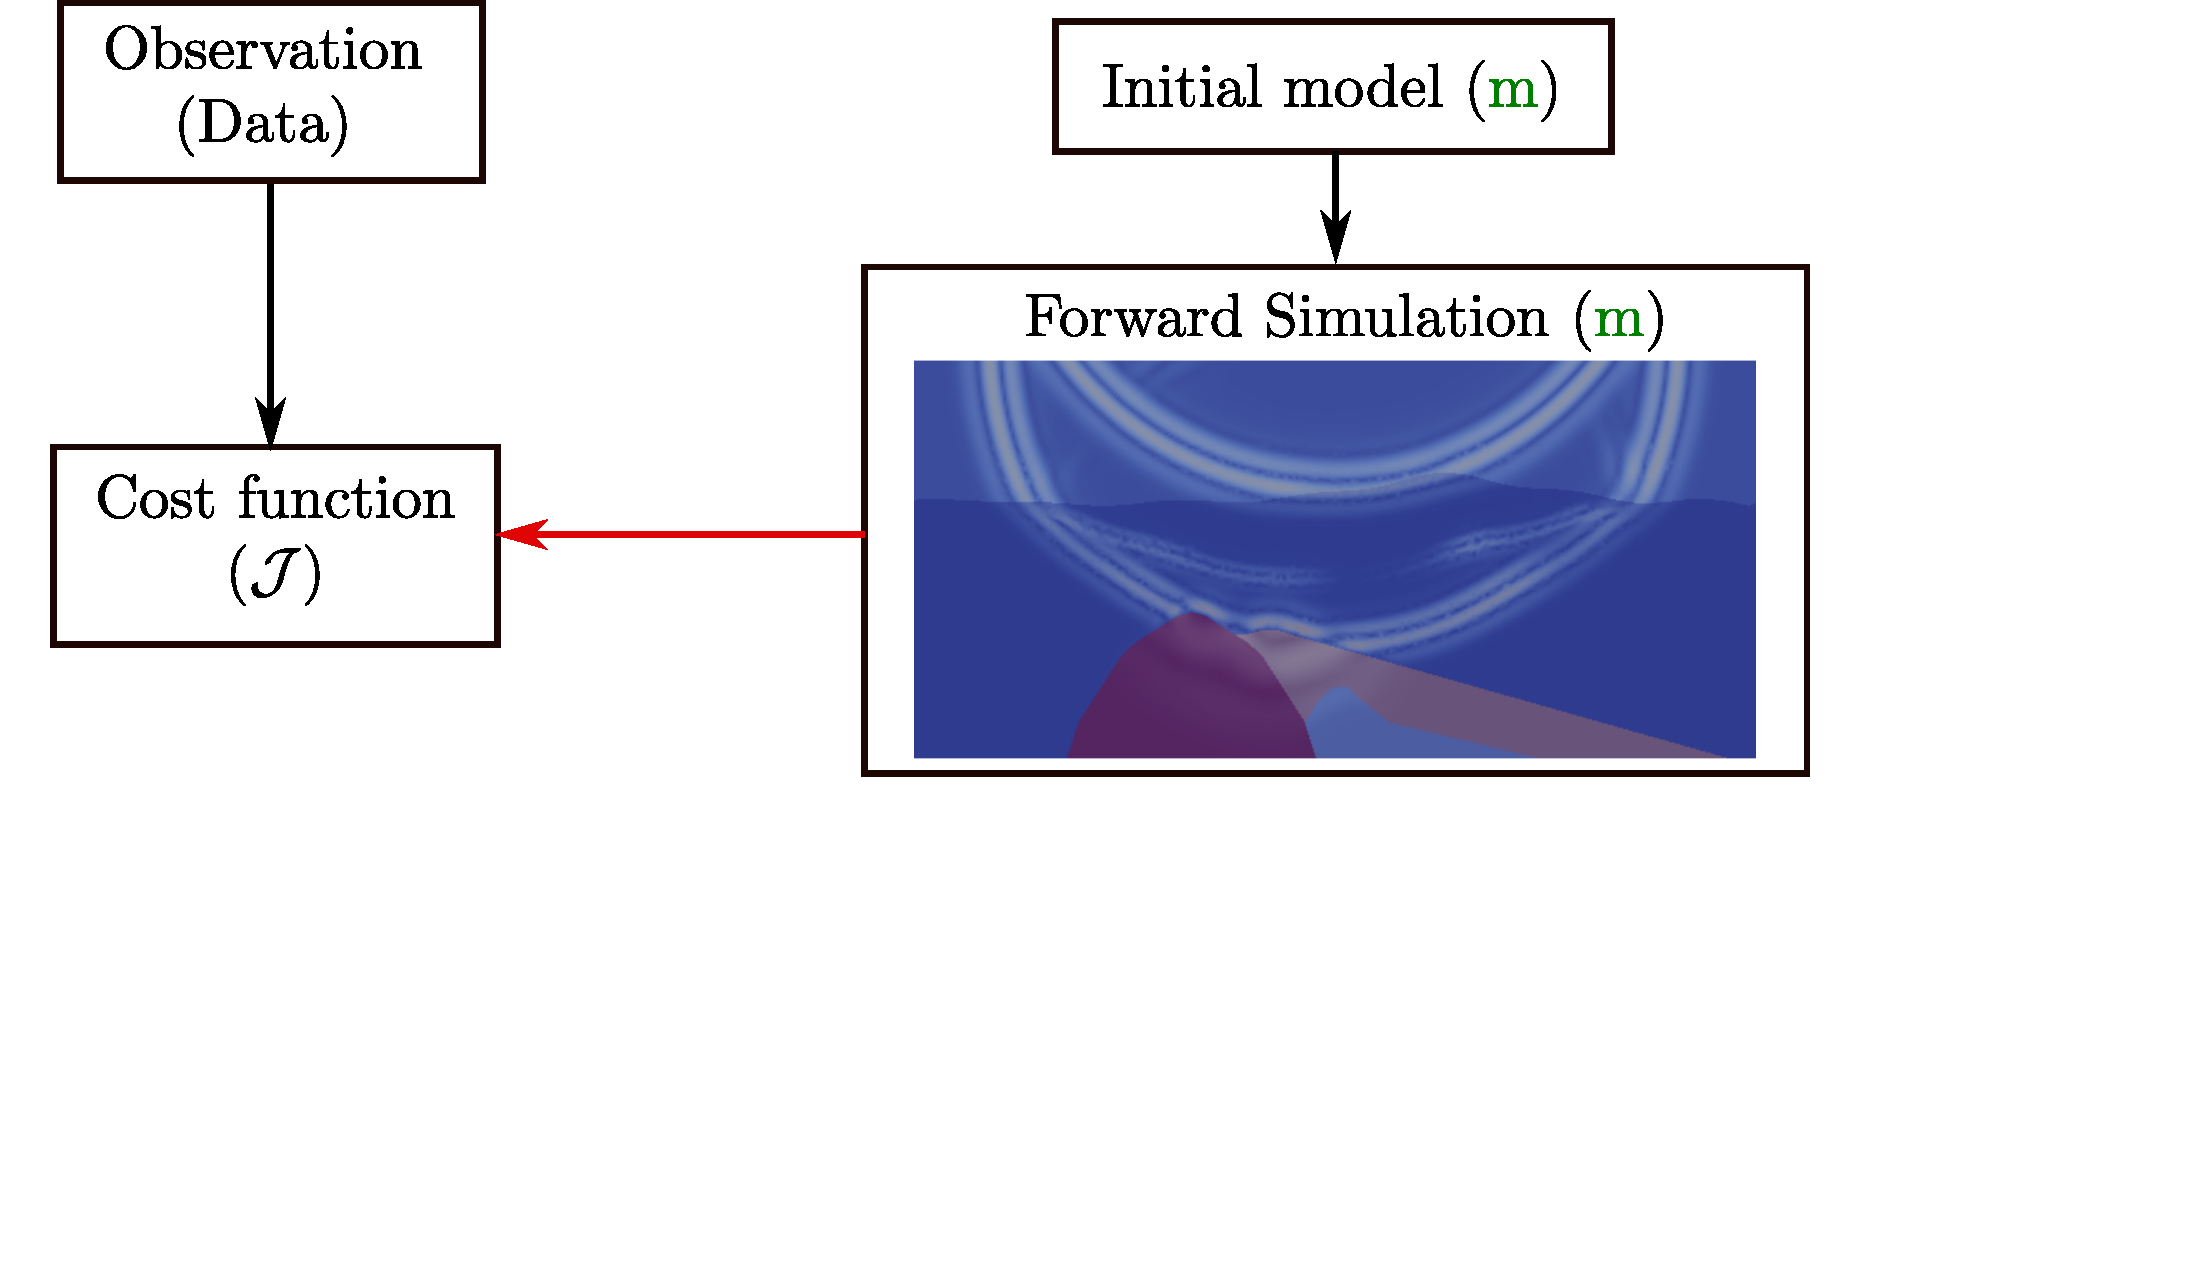
\includegraphics[scale=0.31]{image/fwi_workflow_grad2.pdf}
\end{figure}
\end{frame}

\begin{frame}[noframenumbering]{FWI Workflow}
\begin{figure}
  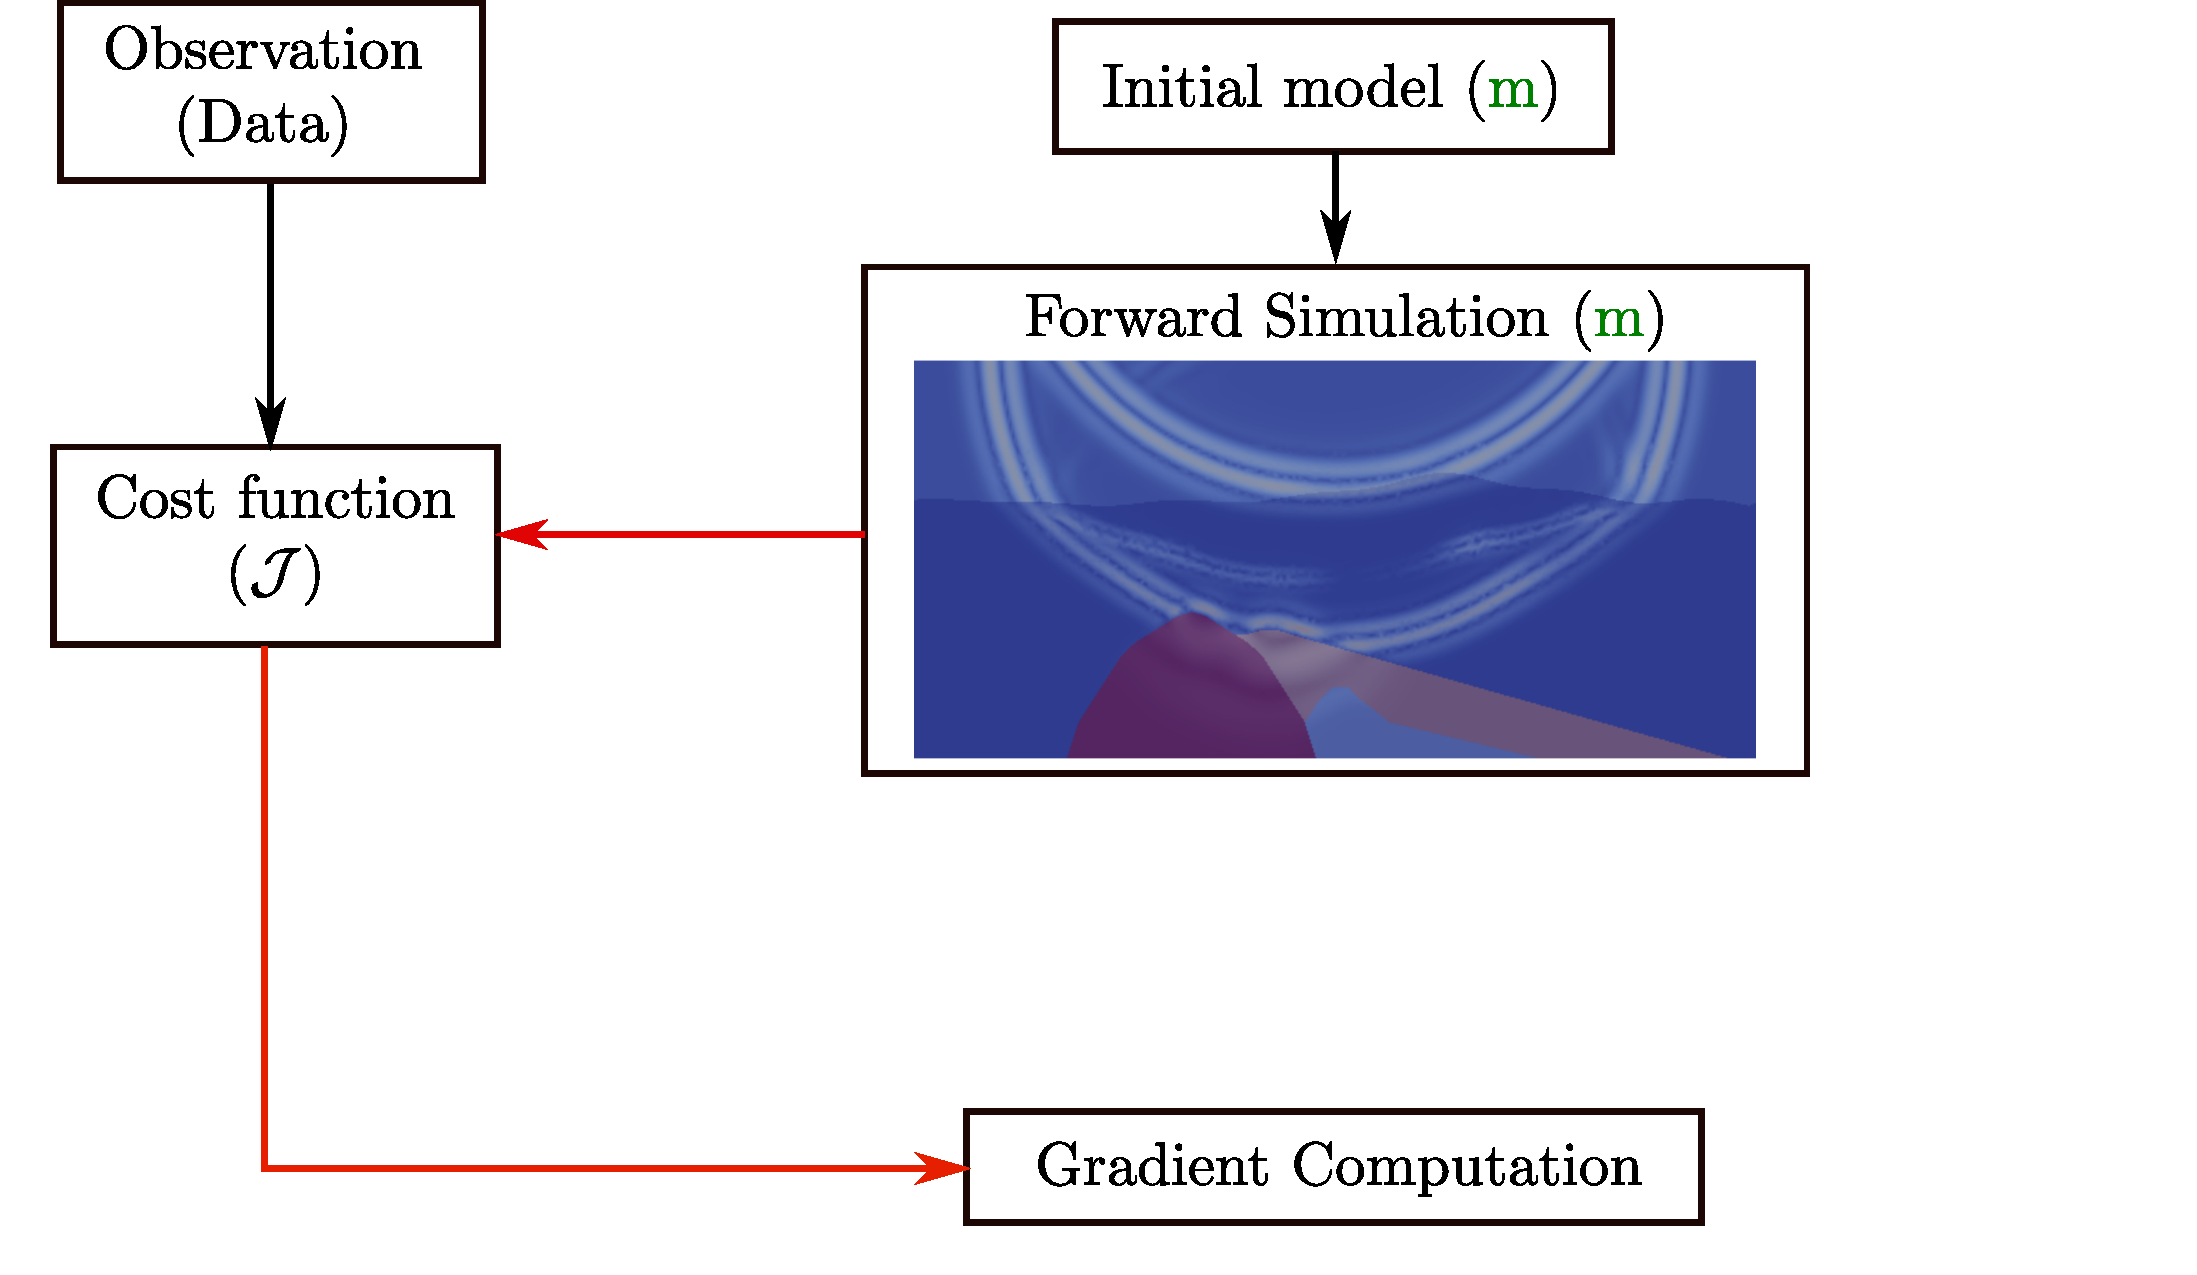
\includegraphics[scale=0.31]{image/fwi_workflow_grad1.pdf}
\end{figure}
\end{frame}

\begin{frame}[noframenumbering]{FWI Workflow}
\begin{figure}
  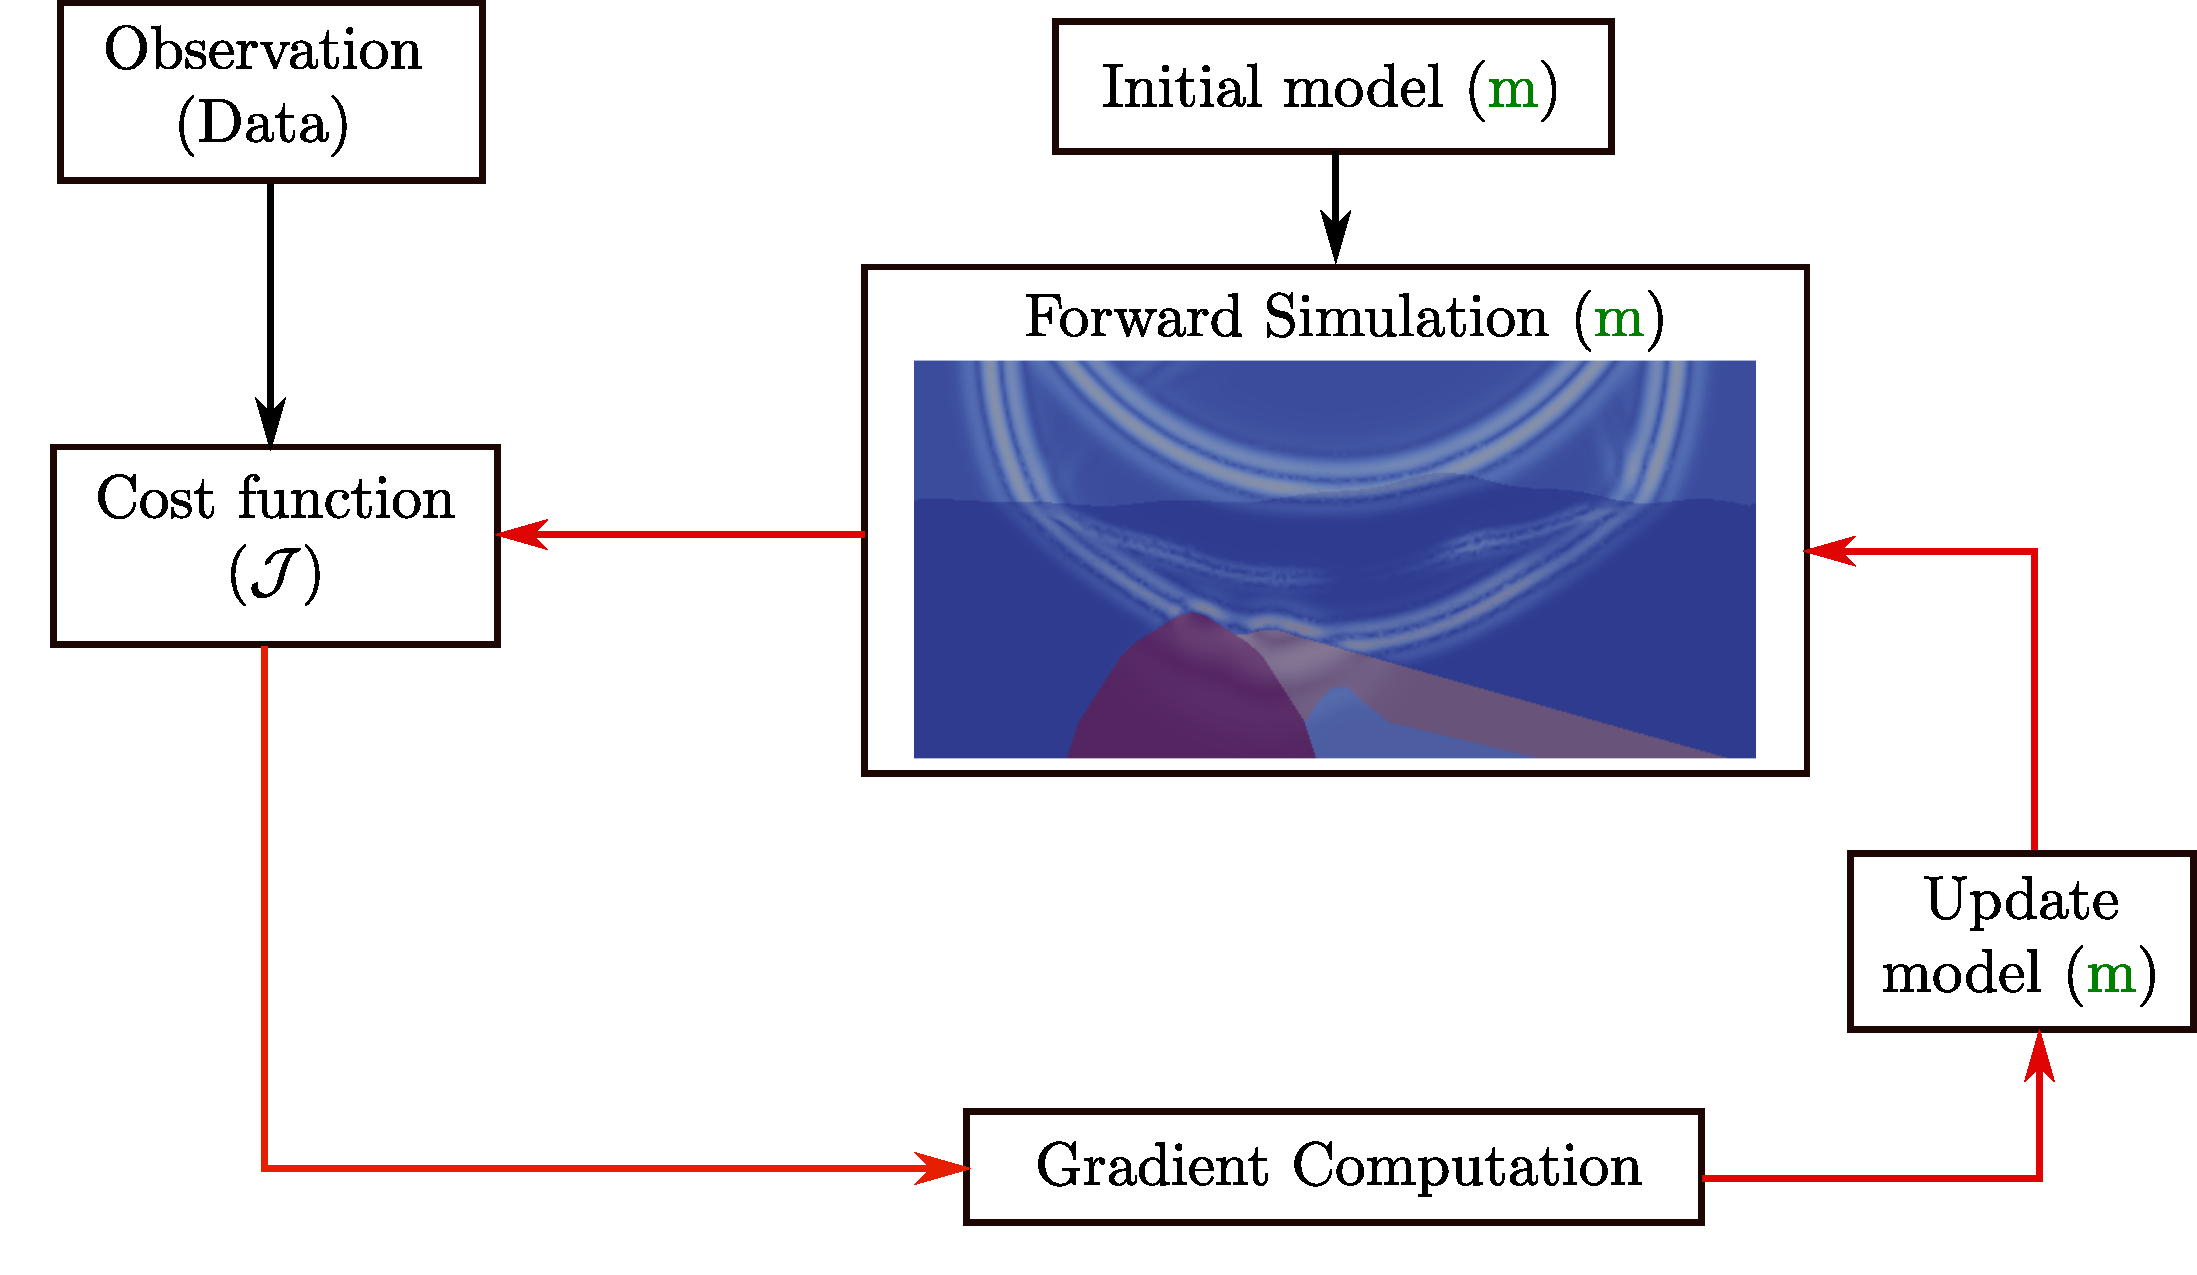
\includegraphics[scale=0.31]{image/fwi_workflow_grad.pdf}
\end{figure}
\end{frame}

\begin{frame}[noframenumbering]{FWI Workflow}
\begin{figure}
  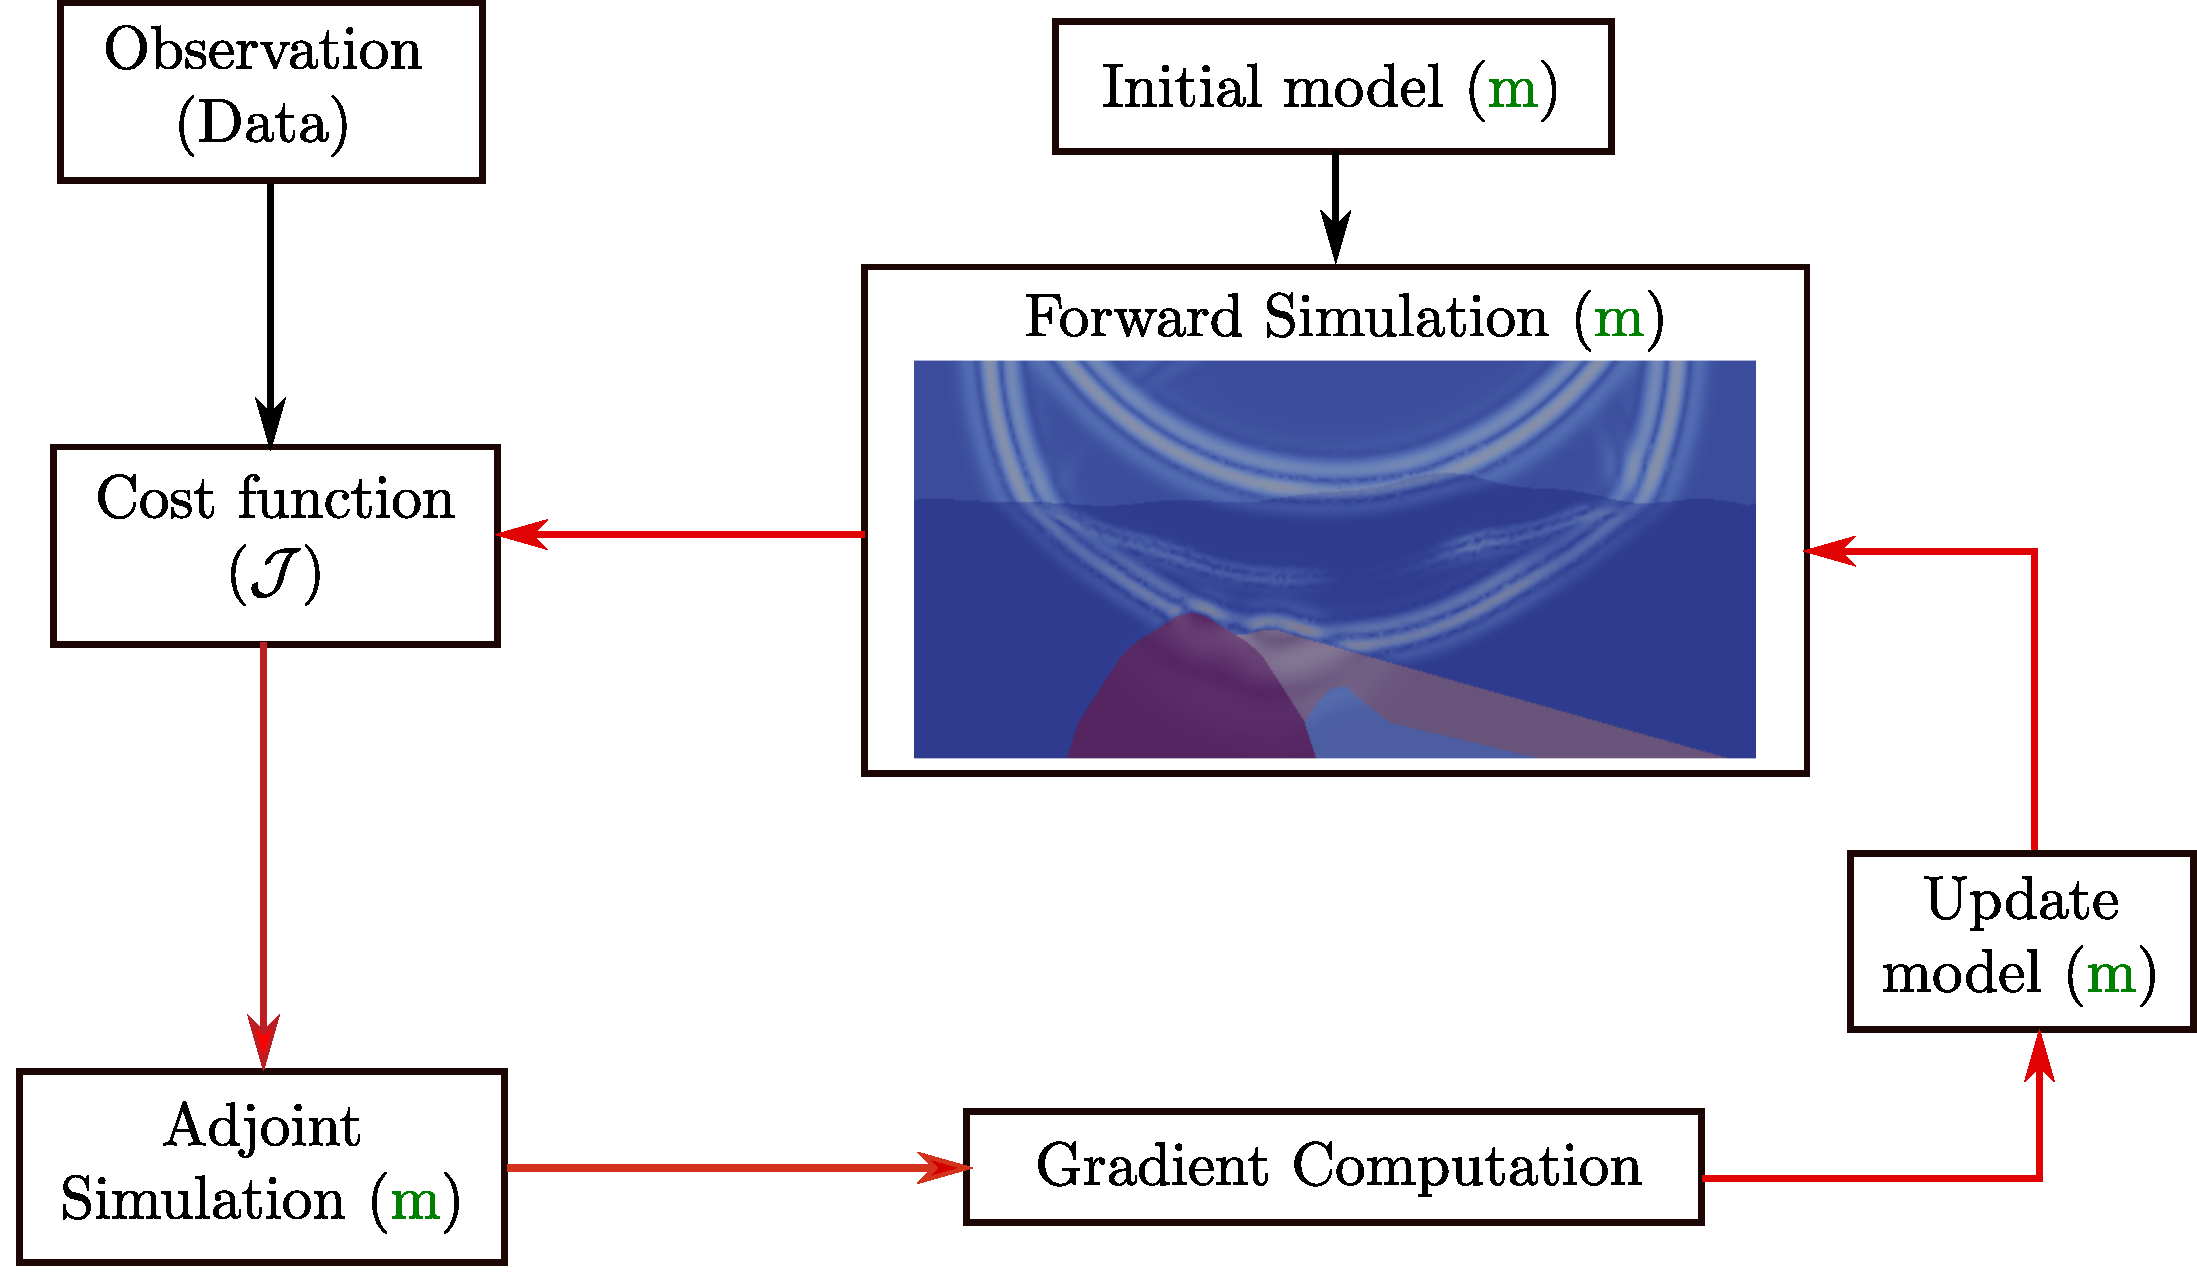
\includegraphics[scale=0.31]{image/fwi_workflow.pdf}
\end{figure}
\end{frame}

\begin{frame}[noframenumbering]{FWI Workflow}
\begin{figure}
  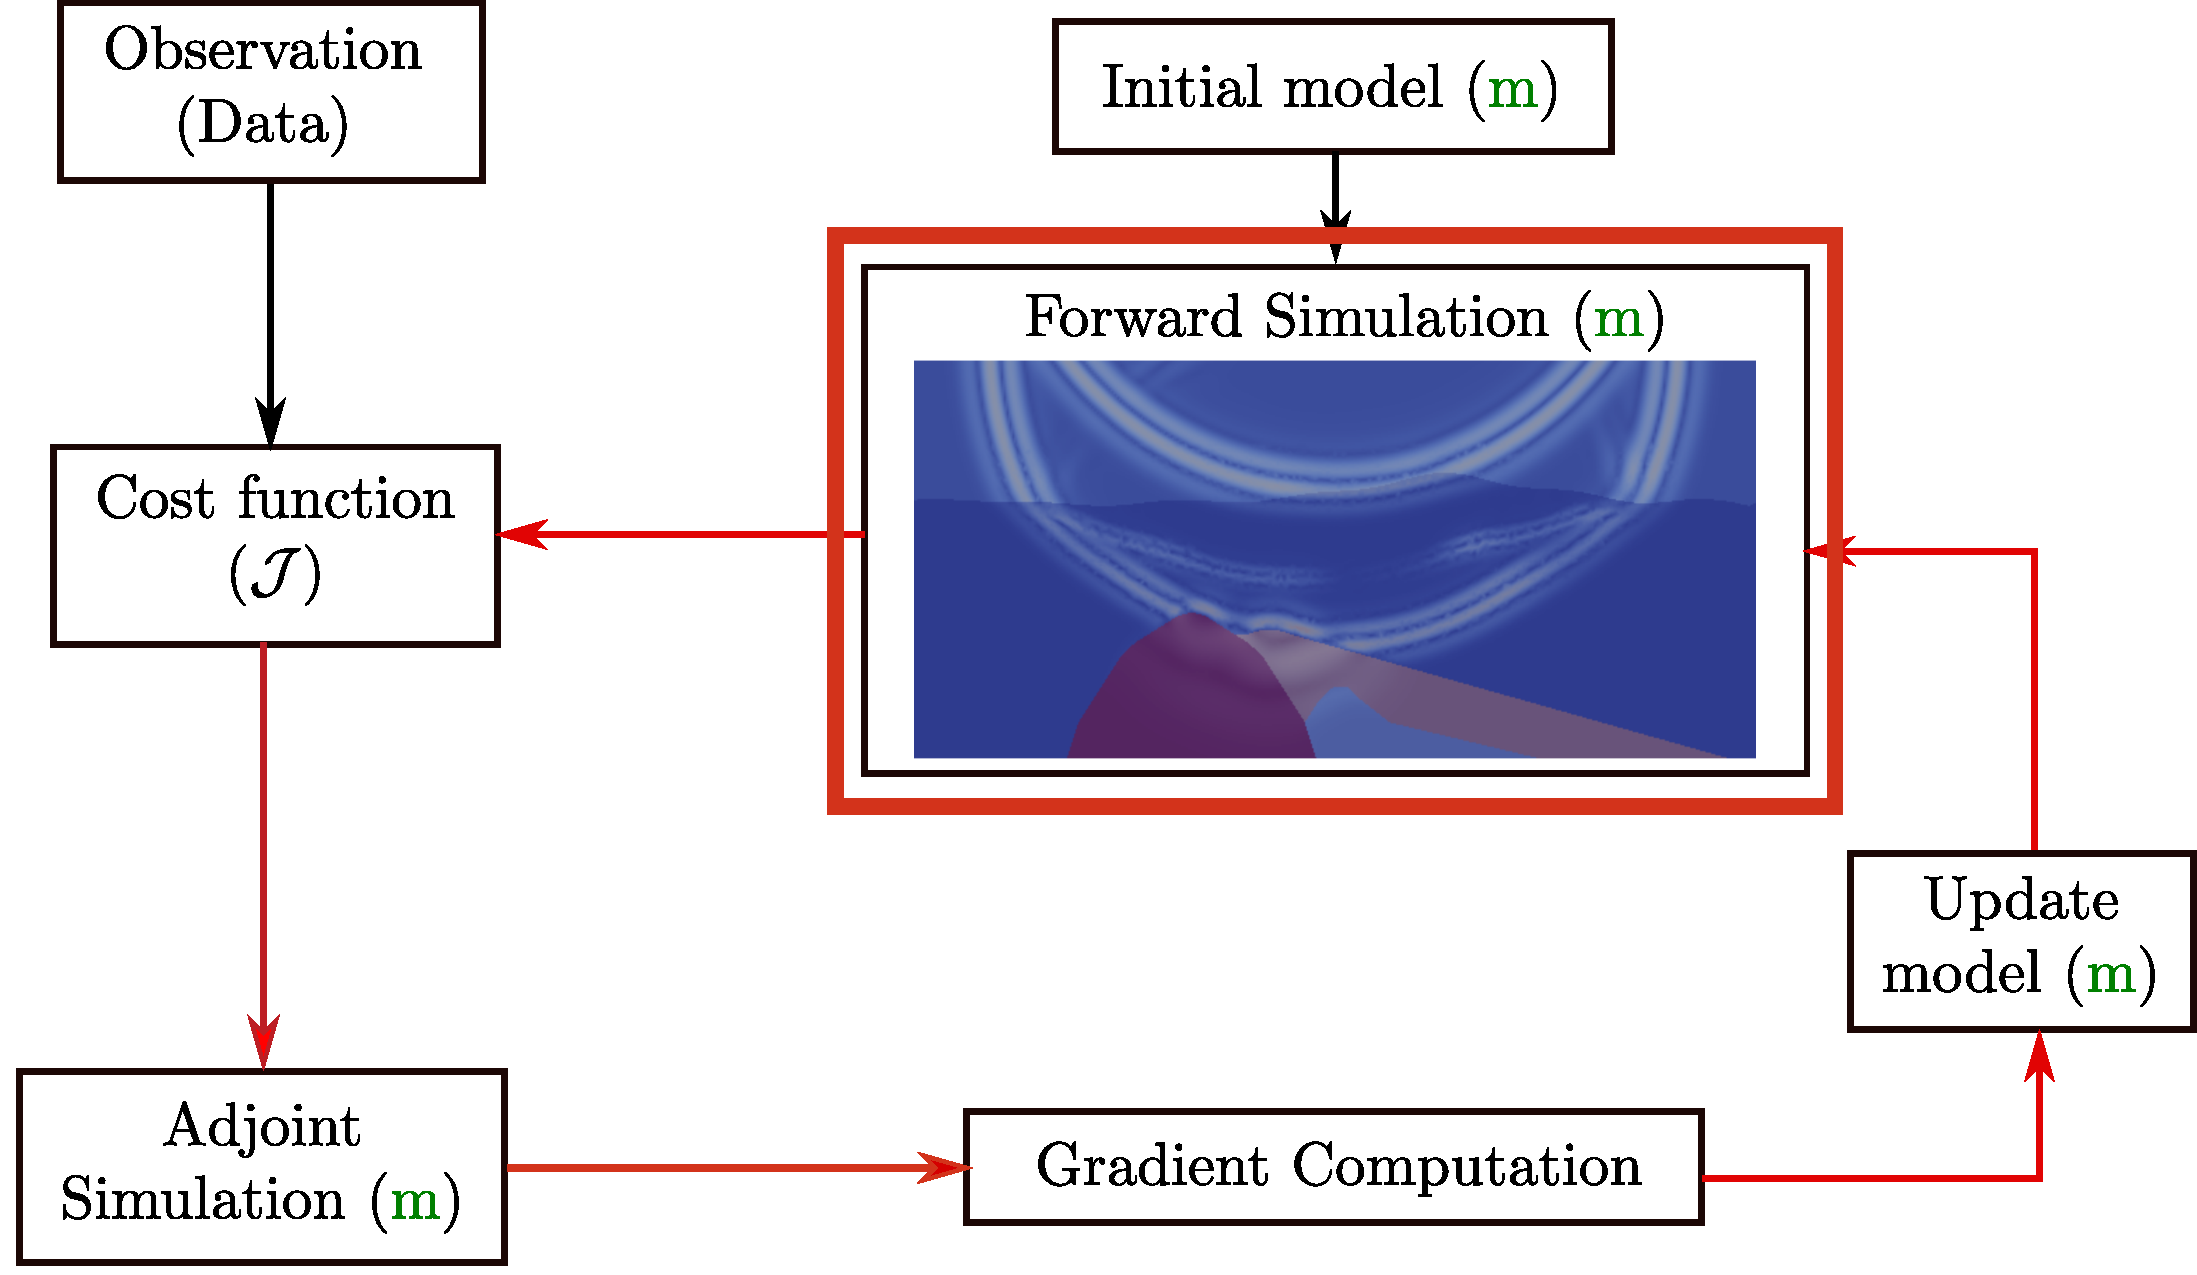
\includegraphics[scale=0.31]{image/fwi_workflow_red.pdf}
\end{figure}
\end{frame}
  %% intro FWI
  % ============================================
% ====== Frame : Plan ========================
% ============================================
{
  \AtBeginSection[]{}
}


% ============================================
% ====== Frame : Continuous model    =========
% ============================================

\section{Forward Discretization}
\subsection{The continuous model}
\begin{frame}{Continuous Forward Model}
  \small
  First order acoustic wave equation:
  \vspace{-0.7cm}
  \begin{multicols}{2}
  \begin{empheq}[left=\empheqlbrace]{align}
    & \frac{1}{\density \velocity^2}\frac{\partial \contP}{\partial t}+\nabla \cdot \contV=f_p \text{~~ on $\boldsymbol{\Omega}$}\\
    & \density\frac{\partial \contV}{\partial t}+\nabla\contP=0  \text{~~ on $\boldsymbol{\Omega}$}\\
    & \contP=0 \text{~~ on $\textcolor{\myred}{\boldsymbol{\Gamma_1}}$} \\
    & \contP - \velocity \density \contV \cdot \normal=0 \text{~~ on $\textcolor{\myblue}{\boldsymbol{\Gamma_2}}$} \\
    & \contP(0) = 0 \text{, ~~~} \contV(0) = 0
  \end{empheq}

  \columnbreak

~ \\
\begin{center}
\renewcommand\tikzscale{1.0}
\begin{figure}[H]
\centering
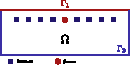
\includegraphics[scale=2.5]{image/truncated_domain.pdf}
\caption*{Truncated infinite domain.} \label{truncated_domain}
\end{figure}
  \end{center}
  \end{multicols}

\vspace{-0.5cm}
\begin{block}{Quantities of interest:}

\begin{multicols}{2}

\begin{itemize}
\item $\contP$: the pressure (kg.m$^{-1}$.s$^{-2}$)
\item $\contV$: the wavespeed  (m.s$^{-1}$)
\end{itemize}

\columnbreak

\begin{itemize}
\item $\velocity$: velocity  (m.s$^{-1}$)
\item $\density$:  density  (kg.m$^{-3}$)
\item $\bm$:       bulk modulus ($\bm = \density  \velocity^2$) (kg.m$^{-1}$.s$^{-2}$)
\end{itemize}

\end{multicols}
\end{block}

\end{frame}

% ===================================================
% ====== Frame : Discontinuous Galerkin method ======
% ===================================================
\subsection{Discontinuous Galerkin method}
\begin{frame}{Discontinuous Galerkin method}
\vspace{-1.5cm}
Spatial discretization based on Discontinuous Galerkin methods:
\vspace{0.5cm}
\begin{itemize}
\item<1-> Approximation made with discontinuous basis functions
\item<2-> Block diagonal mass matrix
\item<3-> High scalability of the solver \footcite{shraggeSolving3DAcoustic2014} (suitable for HPC environnement)
\item<4-> Deals with unstructured grid (triangles / tetrahedra)
\item<5-> Natural $hp$-adaptivity
\end{itemize}

\begin{overprint}
\onslide<5>
 \begin{multicols}{2}
   \begin{figure}[H]
     \centering
     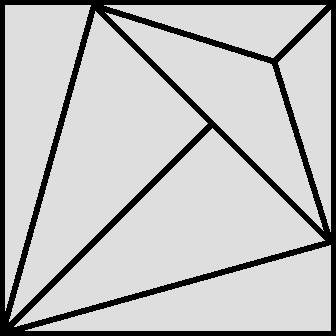
\includegraphics[scale=0.3]{image/h_adaptivity.pdf}
     \caption*{Illustration of \\ $h$-adaptivity.}
     \label{p_adapt_sketch}
   \end{figure}
   \columnbreak
   \begin{figure}[H]
     \centering
     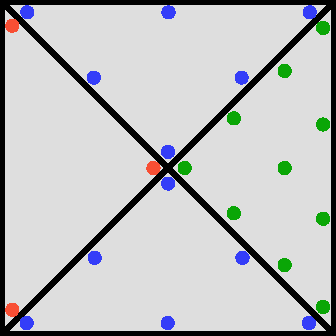
\includegraphics[scale=0.3]{image/p_adaptivity.pdf}
     \caption*{Illustration of \\ $p$-adaptivity.}
     \label{h_adapt_sketch}
   \end{figure}
 \end{multicols}

\onslide<2-4>

\scriptsize
  \begin{empheq}[left=\empheqlbrace]{align}
  & \frac{1}{\bm} \Mass^\element  \frac{\partial \textcolor{\myred}{\coefPolP}^\element}{\partial t}
  + \sum_{d=1}^\dim \Stiff_\xd^\element \textcolor{\myred}{\coefPolVd}^\element
  + \sum_{\Edge} \Mass_\Edge^\element \FluxP^\Edge(\textcolor{\myred}{\coefPolP},\textcolor{\myred}{\coefPolV})
  = \frac{1}{\bm} \Mass^\element \coefpolSource^\element, \\
  & \density \Mass^\element  \frac{\partial \textcolor{\myred}{\coefPolV_d}^\element}{\partial t}
  + \Stiff_\xd^\element \textcolor{\myred}{\coefPolP}^\element + \sum_\Edge \Mass_\Edge \FluxV_d^\Edge (\textcolor{\myred}{\coefPolP},\textcolor{\myred}{\coefPolV})
  = 0  \qquad\text{(for $d=1\,\,\text{to}\,\,\dim$)} \,.
  \label{local_semi_disc2}
  \end{empheq}
\end{overprint}
\vspace{-5cm}

\end{frame}

% ===================================================
% ====== Frame : Speed up studies ===================
% ===================================================

\setbeamercovered{invisible}
\begin{frame}{Scalability Study}{Comparison DG / FD}
\small
Speed up comparison on a 5s simulation in 3D (9km $\times$ 5km $\times$ 3km):

\setlength{\plotwidth}{7cm}
\setlength{\plotheight}{3.7cm}
\begin{figure}[!htbp]
\centering
    \begin{tikzpicture}
      \begin{axis}[%
          width=\plotwidth, height=\plotheight,,
          at={(0,0)},scale only axis,separate axis lines,
          xlabel={\scriptsize{Number of CPU}},
          ylabel={\scriptsize{Speed-up}},
          xmin=1,xmax=768,
%          ymin=0,ymax=1,
          legend pos= north west
          %ymin=0.98,ymax=1.22
        ]
        \addplot[color=black,mark options={solid}, mark=triangle*,
        line width=1.5pt,
        mark size=0pt]
        table[x=monx,y=mony]
        {graph/ideal_speed_up.txt};
        \addlegendentry{\scriptsize{Ideal Speed-up}}
        \addplot[color=blue!80!black,mark options={solid}, mark=triangle*,smooth,
        line width=1pt,
        mark size=0pt]
        table[x=monx,y=mony]
        {graph/dg_speed_up_pres.txt};
        \addlegendentry{\scriptsize{DG}}
        \addplot[color=red,mark options={solid}, mark=*,
        line width=0.8pt,
        mark size=0pt]
        table[x=monx,y=mony]
        {graph/df_speed_up_pres.txt};
        \addlegendentry{\scriptsize{FD}}
\end{axis}
\end{tikzpicture}
\end{figure}

\vspace{-0.2cm}
\uncover<2->{
\begin{block}{\danger Warning}
\small This is an example to illustrate the DG HPC properties. \\
Further comparisons are required to properly compare the two methods.
\end{block}
}

\end{frame}




% ===================================================
% ====== Frame : Time domain motivation =============
% ===================================================
\subsection{Time-Domain}
\begin{frame}{Time-Domain Motivations}

\begin{itemize}
\item<2-> Frequency domain direct-solvers require very large-scale linear systems to solve \footcite{operto20073d}.
\item<3-> Explicit time-schemes do not require the inversion of large size matrices.
\item<4-> In time domain, intermediate results can be stored on the disk to reduce the memory burden (for gradient computation).
\item<5-> In case of disk storage limitation, checkpointing\footcite{griewankAchievingLogarithmicGrowth1992} strategies exists to reduce the overall storage cost.
\end{itemize}

\end{frame}


% ===================================================
% ====== Frame : Time schemes =======================
% ===================================================

\begin{frame}{Time-schemes}
\scriptsize
Three explicit time-schemes as been studied: \\
\begin{multicols}{3}
\textbf{Runge-Kutta 2}

\columnbreak

\textbf{Runge-Kutta 4}

\columnbreak

\textbf{Adams Bashforth 3}
\end{multicols}

\begin{block}{CFL condition\footnotemark}
Initially, the time step $\deltat$ was not computed in the solver.

\begin{multicols}{2}
\begin{equation}
\deltat = \underset{\elementK}{\min}(\deltat^\elementK)\,,
\end{equation}
\begin{equation}
        \deltat^\elementK \le C \frac{r^\elementK}{\velocity^\elementK p^\elementK}\,.
\end{equation}
\vfill

\columnbreak
\tiny
Where:
\begin{itemize}
\item $C$: the CFL condition;
\item $r^\elementK$: the inner radius of the cell $\elementK$;
\item $\velocity^\elementK$: the wavespeed parameter associated to $\elementK$;
\item $p^\elementK$: the polynomial order of approximation in $\elementK$.
\end{itemize}
\end{multicols}
\end{block}
\footcitetext{hesthavenNodalDiscontinuousGalerkin2007}
\end{frame}


\begin{frame}[noframenumbering]{Time-schemes}
\scriptsize
Three explicit time-schemes as been studied: \\
\begin{multicols}{3}
\textbf{Runge-Kutta 2}

\columnbreak

\textbf{Runge-Kutta 4}

\columnbreak

\textbf{Adams Bashforth 3}
\end{multicols}

\begin{block}{CFL condition}
Initially, the time step $\deltat$ was not computed in the solver.

\begin{multicols}{2}
\begin{equation}
\deltat = \underset{\elementK}{\min}(\deltat^\elementK)\,,
\end{equation}
\begin{equation}
        \deltat^\elementK \le C \frac{r^\elementK}{\velocity^\elementK p^\elementK}\,.
\end{equation}
\vfill

\columnbreak
\tiny
Where:
\begin{itemize}
\item $C$: the CFL condition;
\item $r^\elementK$: the inner radius of the cell $\elementK$;
\item $\velocity^\elementK$: the wavespeed parameter associated to $\elementK$;
\item $p^\elementK$: the polynomial order of approximation in $\elementK$.
\end{itemize}
\end{multicols}
\end{block}
\begin{overprint}
\onslide<1>
\begin{figure}[H]
\centering
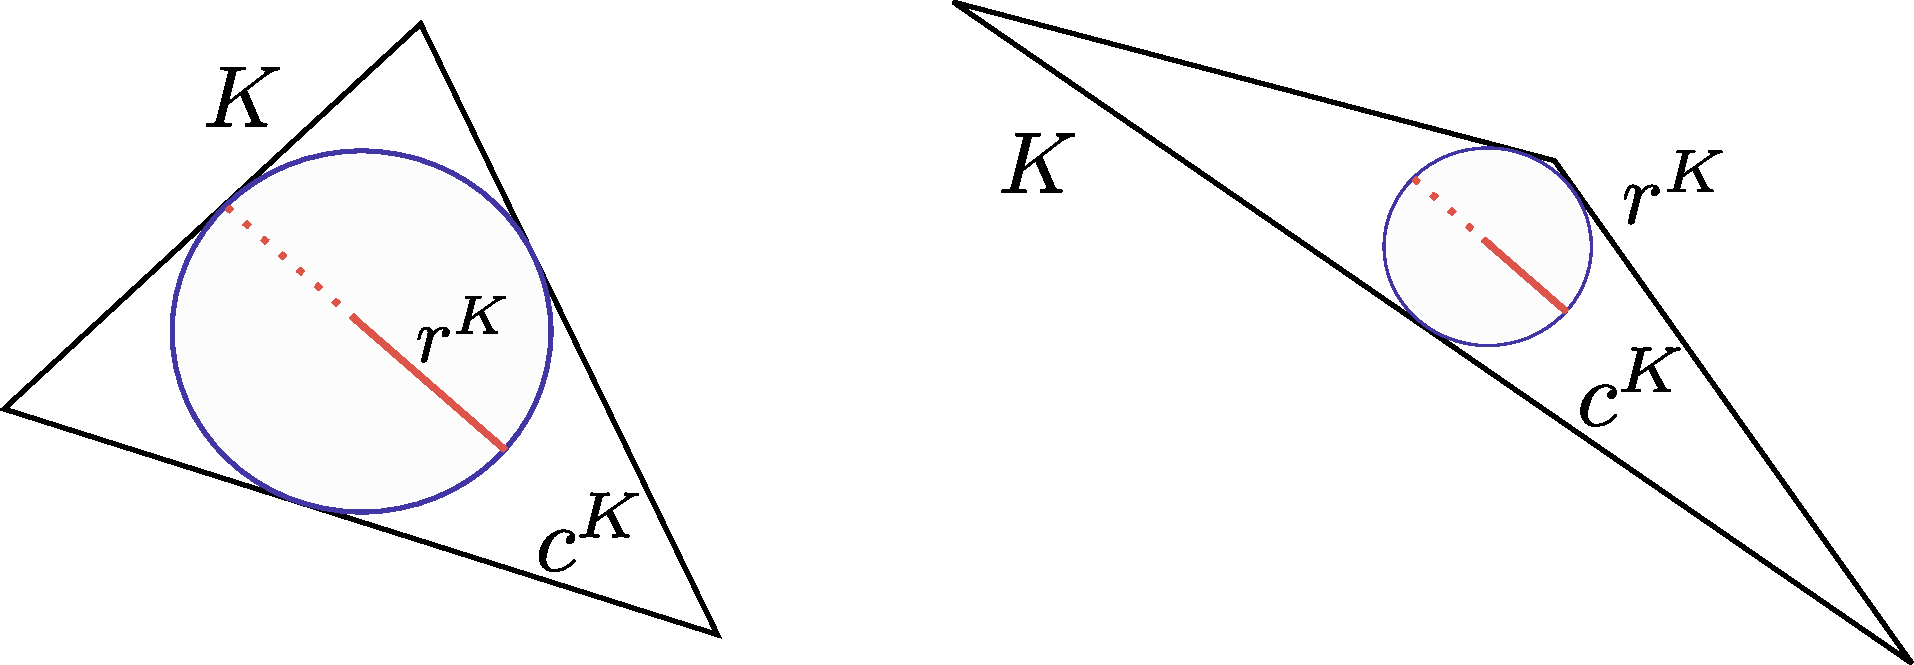
\includegraphics[scale=0.2]{image/cfl.pdf}
\label{cfl_sketch}
\end{figure}
\onslide<2>
\begin{table}[H]
\centering
\begin{tabular}{|l|l|l|l|}
\hline
  & RK2  & RK4  & AB3  \\ \hline
C & 0.66 & 0.84 & 0.18 \\ \hline
\end{tabular}
\caption*{CFL coefficients for different time schemes.}
\label{coef_cfl}
\end{table}
\end{overprint}

\end{frame}


% ============================================
% ====== Frame : Bernstein Bezier    =========
% ============================================

\subsection{Bernstein-Bézier}
 \begin{frame}{Polynomial bases}
 \scriptsize
 Two polynomial bases has been studied:
 \begin{multicols}{2}
 \textbf{Lagrange} (Nodal)

\vspace{0.5cm}
\begin{figure}[H]
\centering
\setlength{\plotwidth}{3.5cm}
\setlength{\plotheight}{2.5cm}
    \begin{tikzpicture}
      \begin{axis}[%
          width=\plotwidth, height=\plotheight,,
          at={(0,0)},scale only axis,separate axis lines,
          xlabel={$x$},
          %%   ymode=log,
          %yminorticks=true,
           xmin=0,xmax=1,
           %ymin=0,ymax=1,
          legend pos=outer north east
          %ymin=0.98,ymax=1.22
        ]

        %% load current data
        %% -----------------
        \addplot[color=blue!50!black,mark options={solid}, mark=triangle*,
          line width=2pt,
          mark size=0pt]
        table[x=x,y=1]
        {graph/lagrange_5.dat};
        \addlegendentry{$\ell_1^5$}

 \addplot[color=red!75!black,mark options={solid}, mark=*,
          line width=2pt,
          mark size=0pt]
        table[x=x,y=2]
        {graph/lagrange_5.dat};
        \addlegendentry{$\ell_2^5$}

 \addplot[color=green!50!black,mark options={solid}, mark=square*,
          line width=2pt,
          mark size=0pt]
        table[x=x,y=3]
        {graph/lagrange_5.dat};
        \addlegendentry{$\ell_3^5$}

 \addplot[color=yellow!80!black,mark options={solid}, mark=square*,
          line width=2pt,
          mark size=0pt]
        table[x=x,y=4]
        {graph/lagrange_5.dat};
        \addlegendentry{$\ell_4^5$}

 \addplot[color=green!75!white,mark options={solid}, mark=square*,
          line width=2pt,
          mark size=0pt]
        table[x=x,y=5]
        {graph/lagrange_5.dat};
        \addlegendentry{$\ell_5^5$}

 \addplot[color=blue!40!white,mark options={solid}, mark=diamond*,
          line width=2pt,
          mark size=0pt]
        table[x=x,y=6]
        {graph/lagrange_5.dat};
        \addlegendentry{$\ell_6^5$}
      \end{axis}
      %% --------------------------------------------------------------------
    \end{tikzpicture}

\caption*{\scriptsize{Illustration of $P^5([0,1])$ Lagrange basis.}}
\label{lagrange_5}
\end{figure}

\columnbreak
\textbf{Bernstein-Bézier \footcite{chanGPUacceleratedBernsteinBezierDiscontinuous2016}} (Modal)

\begin{figure}[H]
\centering
\setlength{\plotwidth}{3.5cm}
\setlength{\plotheight}{2.5cm}
    \begin{tikzpicture}
      \begin{axis}[%
          width=\plotwidth, height=\plotheight,,
          at={(0,0)},scale only axis,separate axis lines,
          xlabel={$\xx$},
          %%   ymode=log,
          %yminorticks=true,
           xmin=0,xmax=1,
           ymin=0,ymax=1,
          legend pos=outer north east
          %ymin=0.98,ymax=1.22
        ]

        %% load current data
        %% -----------------
        \addplot[color=blue!50!black,mark options={solid}, mark=triangle*,
          line width=2pt,
          mark size=0pt]
        table[x=x,y=50]
        {graph/bb_5.dat};
        \addlegendentry{$B^5_{5,0}$}

 \addplot[color=red!75!black,mark options={solid}, mark=*,
          line width=2pt,
          mark size=0pt]
        table[x=x,y=41]
        {graph/bb_5.dat};
        \addlegendentry{$B^5_{4,1}$}

 \addplot[color=green!50!black,mark options={solid}, mark=square*,
          line width=2pt,
          mark size=0pt]
        table[x=x,y=32]
        {graph/bb_5.dat};
        \addlegendentry{$B^5_{3,2}$}

 \addplot[color=yellow!80!black,mark options={solid}, mark=square*,
          line width=2pt,
          mark size=0pt]
        table[x=x,y=23]
        {graph/bb_5.dat};
        \addlegendentry{$B^5_{2,3}$}

 \addplot[color=green!75!white,mark options={solid}, mark=square*,
          line width=2pt,
          mark size=0pt]
        table[x=x,y=14]
        {graph/bb_5.dat};
        \addlegendentry{$B^5_{1,4}$}

 \addplot[color=blue!40!white,mark options={solid}, mark=diamond*,
          line width=2pt,
          mark size=0pt]
        table[x=x,y=05]
        {graph/bb_5.dat};
        \addlegendentry{$B^5_{0,5}$}
      \end{axis}
      %% --------------------------------------------------------------------
    \end{tikzpicture}

\caption*{\scriptsize{Illustration of $P^5([0,1])$ Bernstein-Bézier basis.}}
\label{bb_base_5}
\end{figure}

\end{multicols}

\uncover<2->{
  \begin{tikzpicture}[remember picture,overlay]
    \draw [red,ultra thick,rounded corners] (0,0) rectangle (6.2,6.5);
  \end{tikzpicture}
}
\end{frame}



% ============================================
% ====== Frame : 1D BB    ====================
% ============================================

\begin{frame}{1D Results using Bernstein-Bézier polynomial basis:}

\begin{figure}[htbp]
\begin{subfigure}{0.45\textwidth}
\centering
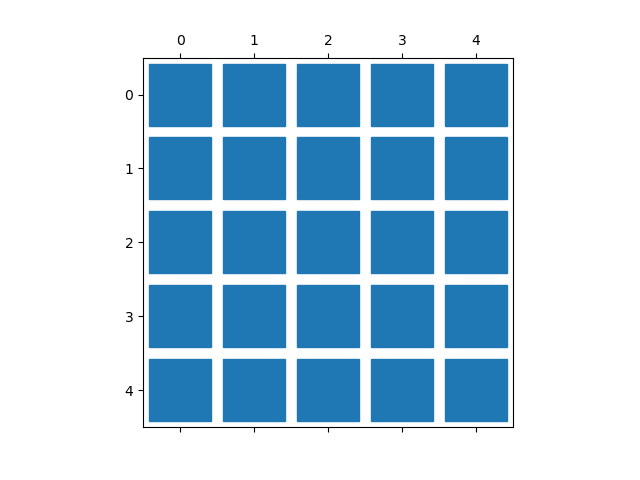
\includegraphics[scale=0.2]{image/dx_lag_4.png}
\caption*{$\Diffx$ for Lagrange and $\PolOrder=4$.}
\end{subfigure}
\begin{subfigure}{0.45\textwidth}
\centering
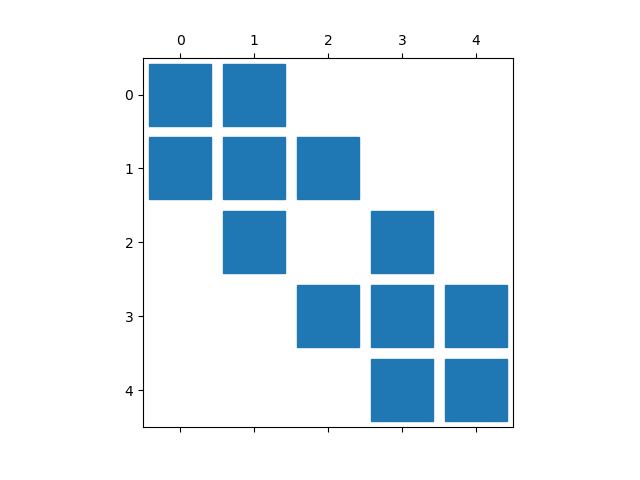
\includegraphics[scale=0.2]{image/dx_bb_4.png}
\caption*{$\Diffx$ for Bernstein and $\PolOrder=4$.}
\end{subfigure}
\begin{subfigure}{0.45\textwidth}
\centering
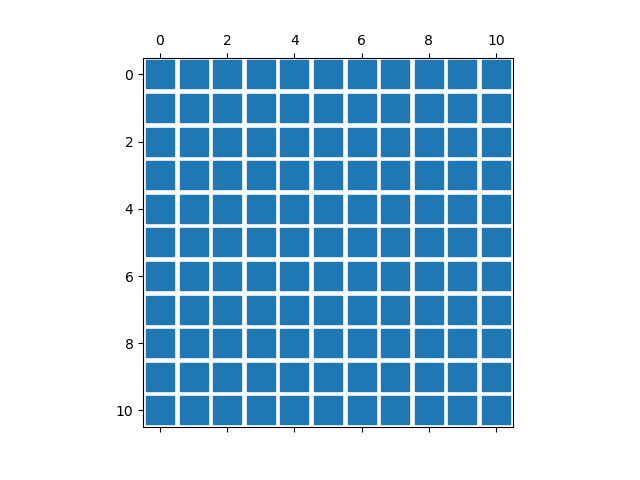
\includegraphics[scale=0.2]{image/dx_lag_10.png}
\caption*{$\Diffx$ for Lagrange and $\PolOrder=10$.}
\end{subfigure}
\begin{subfigure}{0.45\textwidth}
\centering
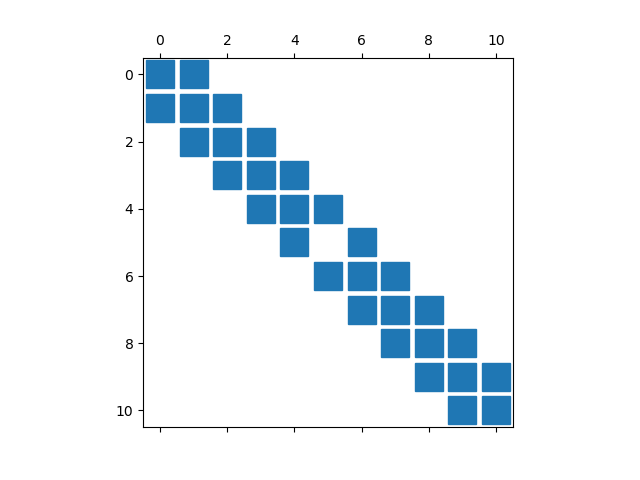
\includegraphics[scale=0.2]{image/dx_bb_10.png}
\caption*{$\Diffx$ for Bernstein and $\PolOrder=10$.}
\end{subfigure}
\caption*{Sparsity comparison between Lagrange and Bernstein
$\Diffx$ operator ($\Diffx =  \MassRef^{-1} \StiffRef_\refxx$).}
\label{dx_sparse_pattern}
\end{figure}
\end{frame}

\begin{frame}[noframenumbering]{1D Results using Bernstein-Bézier polynomial basis:}
\setlength{\plotwidth}{6.0cm}
\setlength{\plotheight}{4.5cm}
\begin{figure}[htbp]
\centering
  %% \begin{subfigure}[b]{0.5\textwidth}
    \begin{tikzpicture}
      \begin{axis}[%
          width=\plotwidth, height=\plotheight,,
          at={(0,0)},scale only axis,separate axis lines,xminorticks=true,
          xlabel={Polynomial order $\PolOrder$},
          ylabel={NZV},
          xmin=0,xmax=21,
          legend pos=north west
        ]
        %% load current data
        %% -----------------
        \addplot[color=blue!50!black,mark options={solid}, mark = triangle,
          line width=1pt,
          mark size=2pt]
        table[x=order,y=nzv]
        {graph/Bernstein_sparse.txt};
        \addlegendentry{Bernstein-Bézier}
        \addplot[color=red!50!black,mark options={solid}, mark = *,
          line width=1pt,
          mark size=2pt]
        table[x=order,y=nzv]
        {graph/Lagrange_sparse.txt};
        \addlegendentry{Lagrange}
        %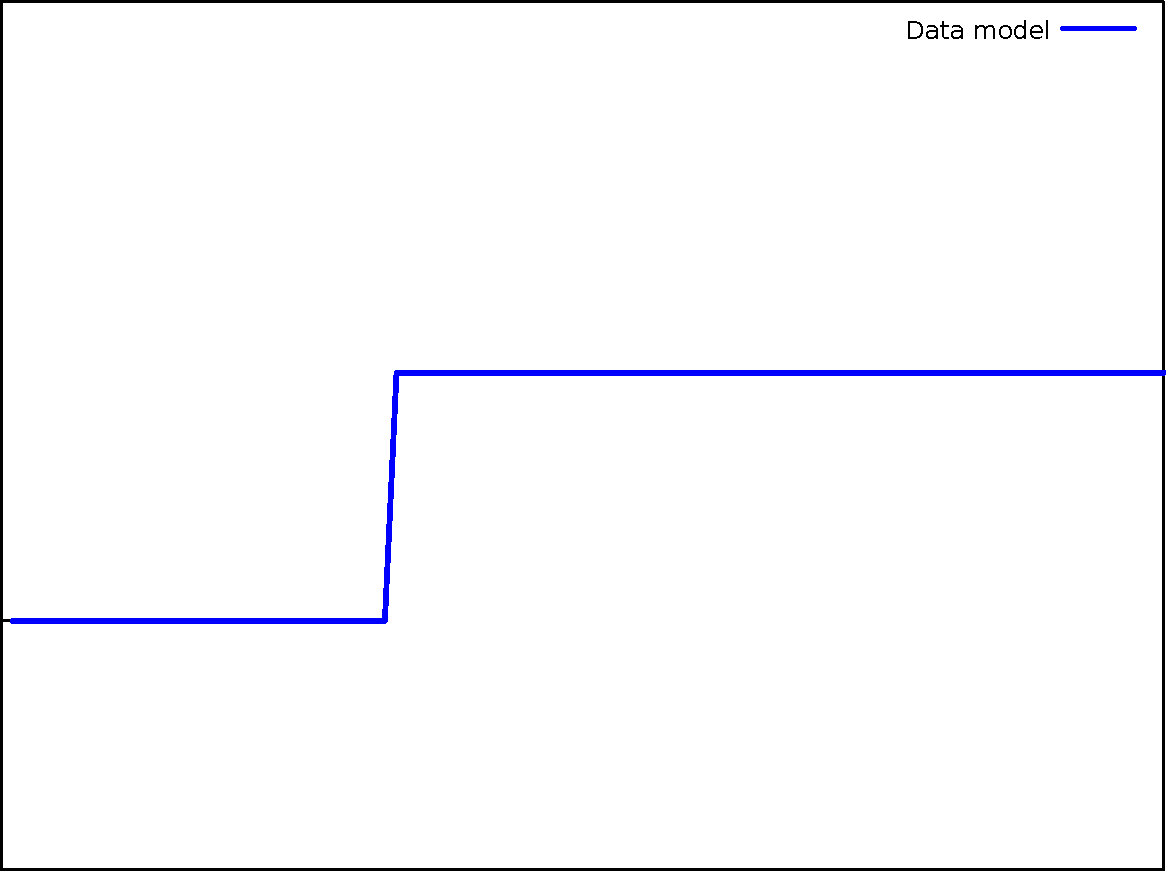
\includegraphics{images/data_bis.pdf}
      \end{axis}
      %% --------------------------------------------------------------------
    \end{tikzpicture}
  %%   \caption{}
  %%   \label{nzv_order}
  %% \end{subfigure}
  %% \begin{subfigure}[b]{0.5\textwidth}
  %%   \setlength{\plotwidth}{6.0cm}
  %%   \setlength{\plotheight}{4.5cm}
  %%   \begin{tikzpicture}
  %%     \begin{axis}[%
  %%         width=\plotwidth, height=\plotheight,,
  %%         at={(0,0)},scale only axis,separate axis lines,xminorticks=true,
  %%         xlabel={Polynomial order $\PolOrder$},
  %%         ylabel={Ratio},
  %%         %%   ymode=log,
  %%         %yminorticks=true,
  %%         xmin=0,xmax=21,
  %%         legend pos=north east
  %%         %ymin=0.98,ymax=1.22
  %%       ]

  %%       %% load current data
  %%       %% -----------------
  %%       \addplot[color=blue!50!black,mark options={solid}, mark = triangle,
  %%         line width=1pt,
  %%         mark size=2pt]
  %%       table[x=order,y=ratio]
  %%       {graph/Bernstein_sparse.txt};
  %%       \addlegendentry{Bernstein-Bézier}
  %%       \addplot[color=red!50!black,mark options={solid}, mark = *,
  %%         line width=1pt,
  %%         mark size=2pt]
  %%       table[x=order,y=ratio]
  %%       {graph/Lagrange_sparse.txt};
  %%       \addlegendentry{Lagrange}
  %%       %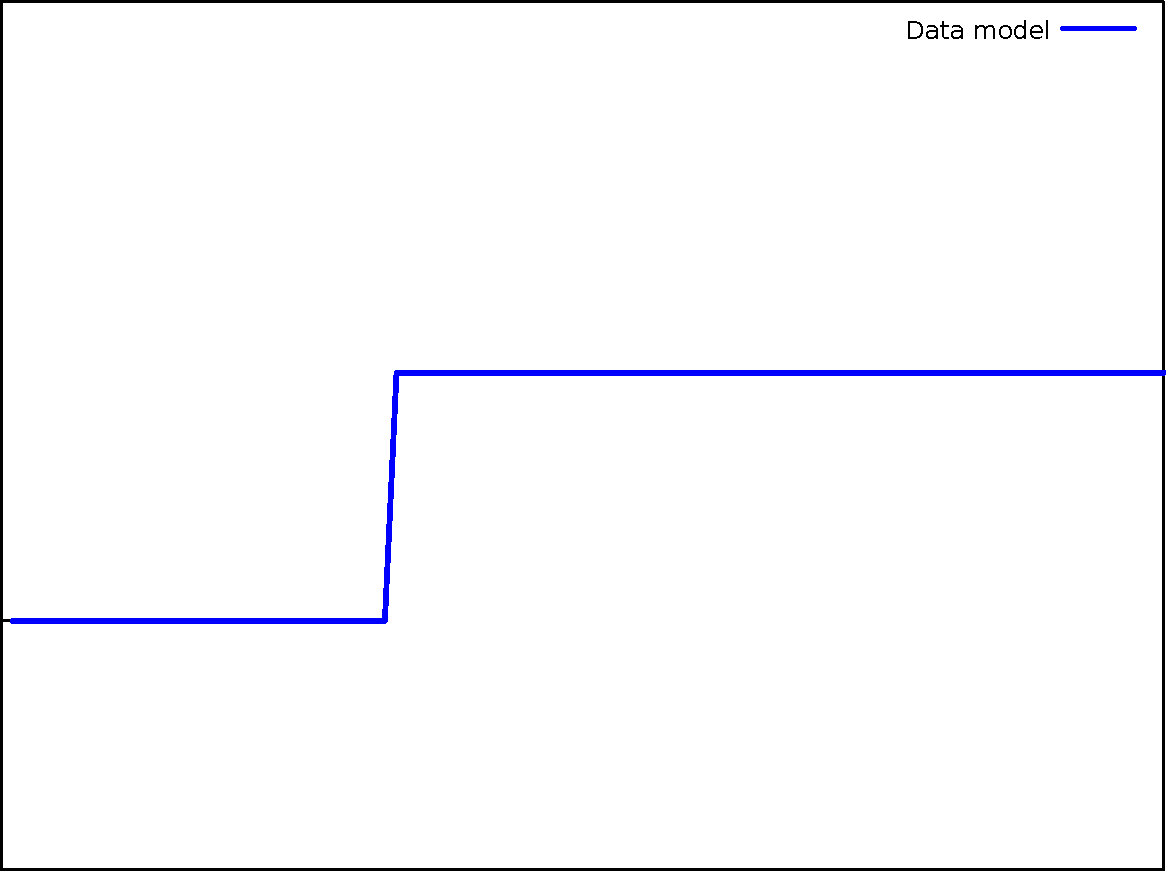
\includegraphics{images/data_bis.pdf}
  %%     \end{axis}
  %%     %% --------------------------------------------------------------------
  %%   \end{tikzpicture}
  %%   \caption{}
  %%   \label{ratio_order}
  %% \end{subfigure}

  \caption*{Non zero values (NZV) of the global volume operator as a function of the polynomial order.}
  \label{bb_lag_comp_1d}
\end{figure}

\end{frame}



\begin{frame}[noframenumbering]{2D and 3D Results using Bernstein-Bézier polynomial basis:}
\scriptsize
\vspace{0.5cm}
\begin{table}[H]
    \centering
    \begin{tabular}{|l|l|l|l|l|l|}
    \hline
        \textbf{Sigsbee (2D)} & P1 & P2 & P3 & P4 & P5 \\ \hline
        Number of elements ($\nbelem$) & 569522 & 243636 & 121235 & 66644 & 35929 \\ \hline
        Nodal CPU time (s) & 20628 & 15938 & 14518 & 14649 & 13471 \\ \hline
        Bernstein Bézier CPU time (s) & 41976 & 27660 & 19944 & 15492 & 10960 \\ \hline
        Ratio total CPU time (BB/Nodal) & \cellcolor{\myred!30}2.0 & \cellcolor{\myred!30}1.7 & \cellcolor{\myred!30}1.4 & \cellcolor{\myred!30}1.1 & \cellcolor{\mygreen!30}0.8 \\ \hline
    \end{tabular}
    \caption*{Global CPU time from nodal and Bernstein simulations on the Sigsbee model.}
    \label{sigsbee_bb_tab}
\end{table}

\uncover<2->{
\begin{table}[H]
    \centering
    \begin{tabular}{|l|l|l|l|l|l|}
    \hline
        \textbf{Seam Foothills (reduced) (3D)} & P1 & P2 & P3 & P4 & P5 \\ \hline
        Number of elements ($\nbelem$)          & 401424 & 122806 & 45932 & 20378 & 11299  \\ \hline
        Nodal CPU time (s)          & 42280  & 43080  & 46920 & 54120  & 69960 \\ \hline
        Bernstein CPU time (s)      & 100080 & 62640  & 43560 & 34200 & 33600   \\ \hline
        Ratio total CPU time (BB/Nodal)     & \cellcolor{\myred!30}2.2 & \cellcolor{\myred!30}1.5 & \cellcolor{\mygreen!30}0.9 & \cellcolor{\mygreen!30}0.6 & \cellcolor{\mygreen!30}0.5 \\ \hline
    \end{tabular}
    \caption*{Global CPU time from nodal and Bernstein simulations
    on the reduced Seam foothills model.}
    \label{seam_bb_tab}
\end{table}
}

\end{frame}


% ============================================
% ====== Frame : WADG     ====================
% ============================================

\subsection{Weight Adjusted Discontinuous Galerkin}

\begin{frame}{Weight Adjusted Discontinuous Galerkin (WADG)}
\scriptsize


\uncover<2->{
  \begin{empheq}[left=\empheqlbrace]{align}
  & \frac{1}{\bm} \Mass^\element  \frac{\partial \textcolor{\myred}{\coefPolP}^\element}{\partial t}
  + \sum_{d=1}^\dim \Stiff_\xd^\element \textcolor{\myred}{\coefPolVd}^\element
  + \sum_{\Edge} \Mass_\Edge^\element \FluxP^\Edge(\textcolor{\myred}{\coefPolP},\textcolor{\myred}{\coefPolV})
  = \frac{1}{\bm} \Mass^\element \coefpolSource^\element, \\
  & \density \Mass^\element  \frac{\partial \textcolor{\myred}{\coefPolV_d}^\element}{\partial t}
  + \Stiff_\xd^\element \textcolor{\myred}{\coefPolP}^\element + \sum_\Edge \Mass_\Edge \FluxV_d^\Edge (\textcolor{\myred}{\coefPolP},\textcolor{\myred}{\coefPolV})
  = 0  \qquad\text{(for $d=1\,\,\text{to}\,\,\dim$)} \,,
  \label{local_semi_disc2}
  \end{empheq}
}

  \uncover<3->{
  [Glinsky and Mercerat]\footcite{merceratNodalHighorderDiscontinuous2015}:
  \begin{equation}
[\Mass^\element_\param]_{i,j} = \int_\element \param(\x) \varphi_i^\element(\x) \varphi_j^\element(\x) d\x. \label{local_mass_mercerat}
  \end{equation}
  }


  \uncover<4->{
[Chan et al.] \footcite{chanWeightadjustedDiscontinuousGalerkin2017}:
  \begin{equation}
(\Mass^\element_\param)^{-1} \approx (\Mwadg^\element_\param)^{-1} = (\Mass^\element)^{-1} \Mass^\element_{1/\param} (\Mass^\element)^{-1}.
\label{inv_wadg}
\end{equation}
}


\end{frame}


% ============================================
% ====== Frame : WADG Quadrature point =======
% ============================================

\begin{frame}{Weight Adjusted Discontinuous Galerkin (WADG)}
  \scriptsize
  For sake of accuracy: $\QuadOrder=2\PolOrder+1$.

\begin{table}[]
\begin{tabular}{|l|l|l|l|l|l|l|}
\hline
Polynomial Order ($\PolOrder$)            & 1 & 2  & 3  & 4  & 5  & 6  \\ \hline
Quadrature Order ($\QuadOrder$)           & 3 & 5  & 7  & 9  & 11 & 13 \\ \hline
Number of quadrature points ($n_q$) in 2D & 6 & 7  & 15 & 19 & 28 & 40 \\ \hline
Number of quadrature points ($n_q$) in 3D & 6 & 14 & 31 & 57 & 95 & 146  \\ \hline
\end{tabular}
\caption*{\scriptsize{Number of quadrature points as a function of $\QuadOrder$.}}
\end{table}


  \begin{figure}[!htbp]
    \begin{subfigure}{0.45\textwidth}
      \centering
      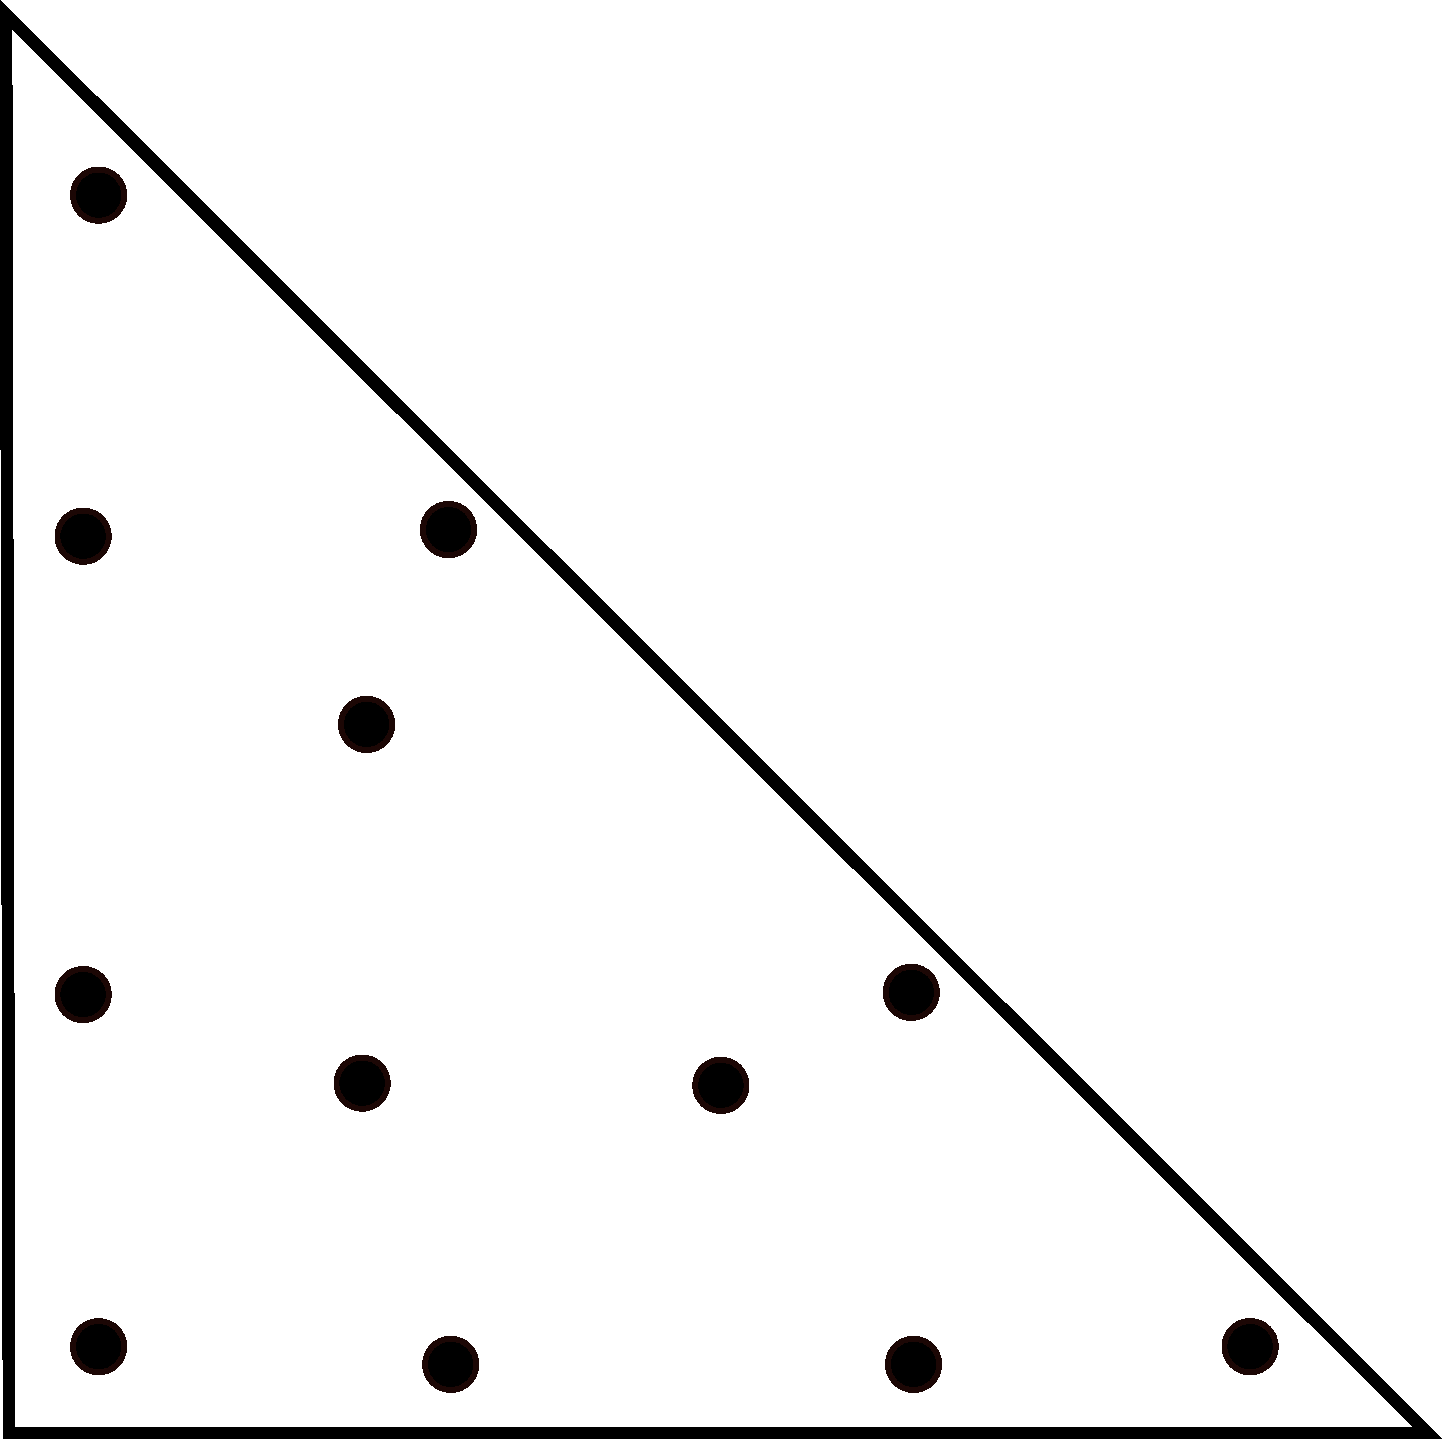
\includegraphics[scale=0.07]{image/quad_2d.pdf}
    \end{subfigure}
    \begin{subfigure}{0.45\textwidth}
      \centering
      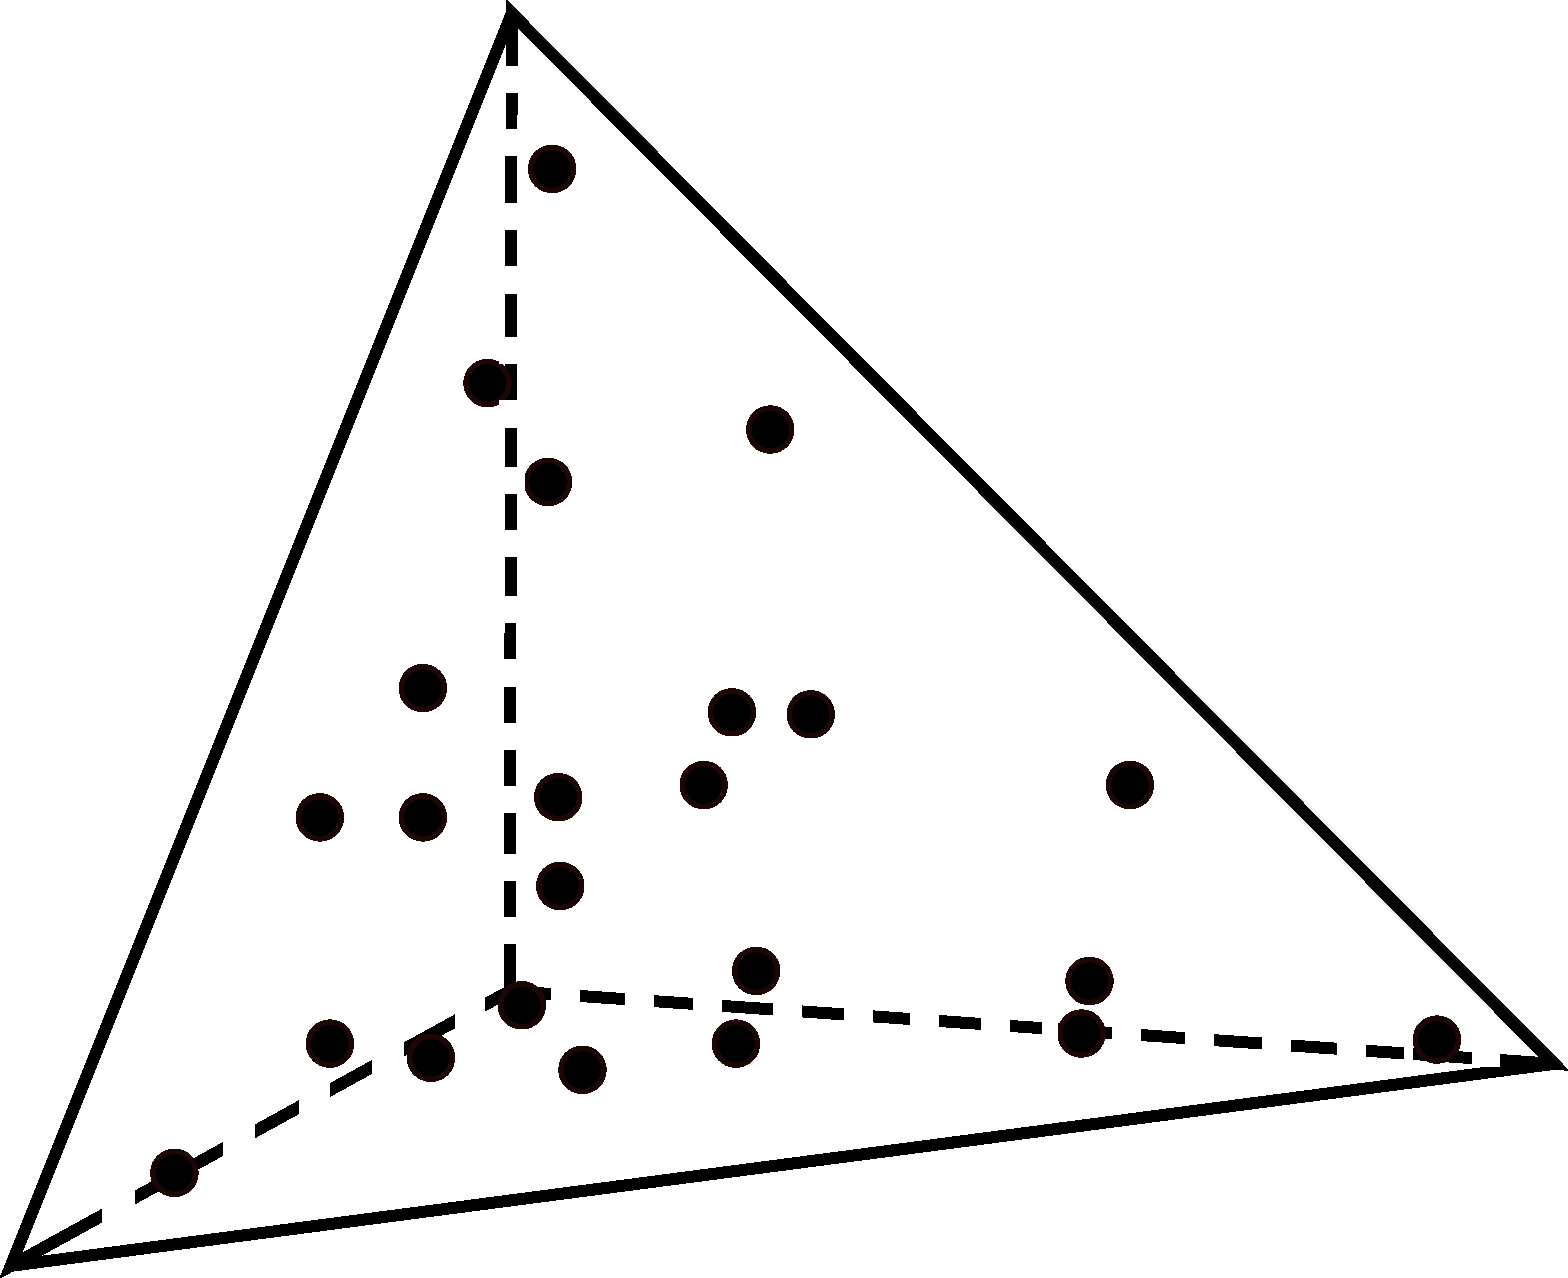
\includegraphics[scale=0.08]{image/quad_3d.pdf}
    \end{subfigure}
    \caption*{\scriptsize{Quadrature points on 2D and 3D reference element for $\QuadOrder=6$.}}
    \label{quad_point_sketch}
  \end{figure}

  \uncover<2->{
  \begin{block}{\danger Warning}
    Such a parametrization requires enhanced output and visualization techniques.
  \end{block}
  }

\end{frame}


% ============================================
% ====== Frame : Semi discrete       =========
% ============================================

\begin{frame}{Semi-discrete formulation}
  \tiny
  \begin{block}{Constant model per element:}
    \begin{empheq}[left=\empheqlbrace]{align}
      & \frac{\partial \textcolor{\myred}{\coefPolP}^\element}{\partial t}
      = -  \bm^\element  \left( \sum_{k=1}^\dim \sum_{d=1}^\dim [J_{T_\element}^{-\top}]_{k,d} \MassRef^{-1}\StiffRef_\refxd \textcolor{\myred}{\coefPolVd}
      -  \sum_{d=1}^\dim \sum_{\Edge \in \element} \frac{\detJF}{\detJK} \MassRef^{-1}\MassRef_\Edge \textcolor{\myred}{\FluxP}^\Edge \right)
      +  \coefpolSource^\element  \\
      & \frac{\partial \textcolor{\myred}{\coefPolVd}^\element}{\partial t} =
      -  \frac{1}{\density}^\element  \left( \sum_{k=1}^\dim [J_{T_\element}^{-\top}]_{k,d} \MassRef^{-1}\StiffRef_\refxd \textcolor{\myred}{\coefPolP}^\element
      - \sum_\Edge \frac{\detJF}{\detJK} \MassRef^{-1}\MassRef_\Edge \textcolor{\myred}{\FluxV}_d^\Edge \right)\,,
      \label{semi_discrete_wadg_operator}
    \end{empheq}
    for $d=1\,\,\text{to}\,\,\dim$. \hfill
  \end{block}

  \tiny
  \begin{block}{Weight Adjusted Discontinuous Galerkin method:}
    \begin{empheq}[left=\empheqlbrace]{align}
      & \frac{\partial \textcolor{\myred}{\coefPolP}^\element}{\partial t}
      = -  \MassRef^{-1} \, \Pquad\, diag(\weight \boldsymbol{\bm}^\element)\, \Pquad^\top  \left( \sum_{k=1}^\dim \sum_{d=1}^\dim [J_{T_\element}^{-\top}]_{k,d} \MassRef^{-1}\StiffRef_\refxd \textcolor{\myred}{\coefPolVd}
      -  \sum_{d=1}^\dim \sum_{\Edge \in \element} \frac{\detJF}{\detJK} \MassRef^{-1}\MassRef_\Edge \textcolor{\myred}{\FluxP}^\Edge \right)
      +  \coefpolSource^\element  \\
      & \frac{\partial \textcolor{\myred}{\coefPolVd}^\element}{\partial t} =
      -  \MassRef^{-1} \, \Pquad\, diag(\weight \boldsymbol{\frac{1}{\density}}^\element)\, \Pquad^\top  \left( \sum_{k=1}^\dim [J_{T_\element}^{-\top}]_{k,d} \MassRef^{-1}\StiffRef_\refxd \textcolor{\myred}{\coefPolP}^\element
      - \sum_\Edge \frac{\detJF}{\detJK} \MassRef^{-1}\MassRef_\Edge \textcolor{\myred}{\FluxV}_d^\Edge \right)\,,
      \label{semi_discrete_wadg_operator}
    \end{empheq}
    for $d=1\,\,\text{to}\,\,\dim$. \hfill
  \end{block}
\end{frame}



% ============================================
% ====== Frame : Cost WADG 2D    =============
% ============================================


\begin{frame}{Computational cost of WADG (2D)}
\colorlet{xcolorA}{red!95!black}
\colorlet{xcolorB}{red!50!black}
\colorlet{ycolorA}{blue!95!black}
\colorlet{ycolorB}{blue!50!black}


\begin{figure}[H]
\centering
\begin{tikzpicture}[scale=0.7]
  \pgfplotsset{ybar stacked, ymin=0, ymax=200, xmin=1.5, xmax=5.5, xtick=data, xlabel= Polynomial Order $\PolOrder$, ylabel=\% of CPU time,
  }
  \begin{axis}[bar shift=-8pt,
    legend pos = outer north east, legend style = {name = serieA},
    ylabel]
    \addplot [draw=ycolorA, pattern= north west lines, pattern color=ycolorA, fill=ycolorA] table [x index = 0, y index = 1] {./graph/num_exp_1/serieA.dat};
    \addplot [draw=blue, pattern=horizontal lines light blue,fill=xcolorA] table [x index = 0, y index = 2] {./graph/num_exp_1/serieA.dat};
    \legend{RHS CPU time (WADG), Apply model CPU time (WADG)}
    \legend{Surface + Volume ($\QuadOrder = 1$), Apply model ($\QuadOrder = 1$)}
  \end{axis}
  \begin{axis}[bar shift = 8pt,
    legend style = {at = {([yshift = -3.5mm, xshift = -3.7mm]serieA.south west)},
      anchor = north west}]
    \addplot [pattern color=ycolorB, pattern=north east lines,fill=ycolorB] table [x index = 0, y index = 1] {./graph/num_exp_1/serieB.dat};
    \addplot [draw=xcolorB, pattern=dots, pattern color=xcolorB, fill=xcolorB] table [x index = 0, y index = 2] {./graph/num_exp_1/serieB.dat};
    \legend{Surface + Volume ($\QuadOrder = 2\PolOrder+1$), Apply model ($\QuadOrder = 2\PolOrder+1$)}
  \end{axis}
\end{tikzpicture}
\caption*{Histogram illustrating the computational proportion of the model operators in
the time derivative evaluation in 2D.}
\label{histo_wadg}
\end{figure}

\end{frame}



% ============================================
% ====== Frame : Cost WADG 3D    =============
% ============================================

\begin{frame}{Computational cost of WADG (3D)}
\colorlet{xcolorA}{red!95!black}
\colorlet{xcolorB}{red!50!black}
\colorlet{ycolorA}{blue!95!black}
\colorlet{ycolorB}{blue!50!black}


\begin{figure}[H]
\centering
\begin{tikzpicture}[scale=0.7]
  \pgfplotsset{ybar stacked, ymin=0, ymax=180, xmin=1.5, xmax=4.5, xtick=data, xlabel=Polynomial order $\PolOrder$, ylabel=\% of CPU time,
  }
  \begin{axis}[bar shift=-8pt,
    legend pos = outer north east, legend style = {name = serieA},
    ylabel]
    \addplot [draw=ycolorA, pattern= north west lines, pattern color=ycolorA, fill=ycolorA] table [x index = 0, y index = 1] {./graph/num_exp_1/serieA_3D.dat};
    \addplot [draw=blue, pattern=horizontal lines light blue, fill=xcolorA] table [x index = 0, y index = 2] {./graph/num_exp_1/serieA_3D.dat};
    \legend{RHS CPU time (WADG), Apply model CPU time (WADG)}
    \legend{Surface + Volume ($\QuadOrder = 1$), Apply model ($\QuadOrder = 1$)}
  \end{axis}
  \begin{axis}[bar shift = 8pt,
    legend style = {at = {([yshift = -3.5mm,xshift = -3.7mm]serieA.south west)},
      anchor = north west}]
    \addplot [pattern color=xcolorA, pattern=north east lines,fill=ycolorB] table [x index = 0, y index = 1] {./graph/num_exp_1/serieB_3D.dat};
    \addplot [draw=xcolorB, pattern=dots, pattern color=xcolorB, fill=xcolorB] table [x index = 0, y index = 2] {./graph/num_exp_1/serieB_3D.dat};
    \legend{Surface + Volume ($\QuadOrder = 2\PolOrder+1$), Apply model ($\QuadOrder = 2\PolOrder+1$)}
  \end{axis}
\end{tikzpicture}
\caption*{Histogram illustrating the computational proportion of the model operators in
the time derivative evaluation in 3D.}
\label{histo_wadg_3D}
\end{figure}
\end{frame}


\begin{frame}
\begin{figure}
  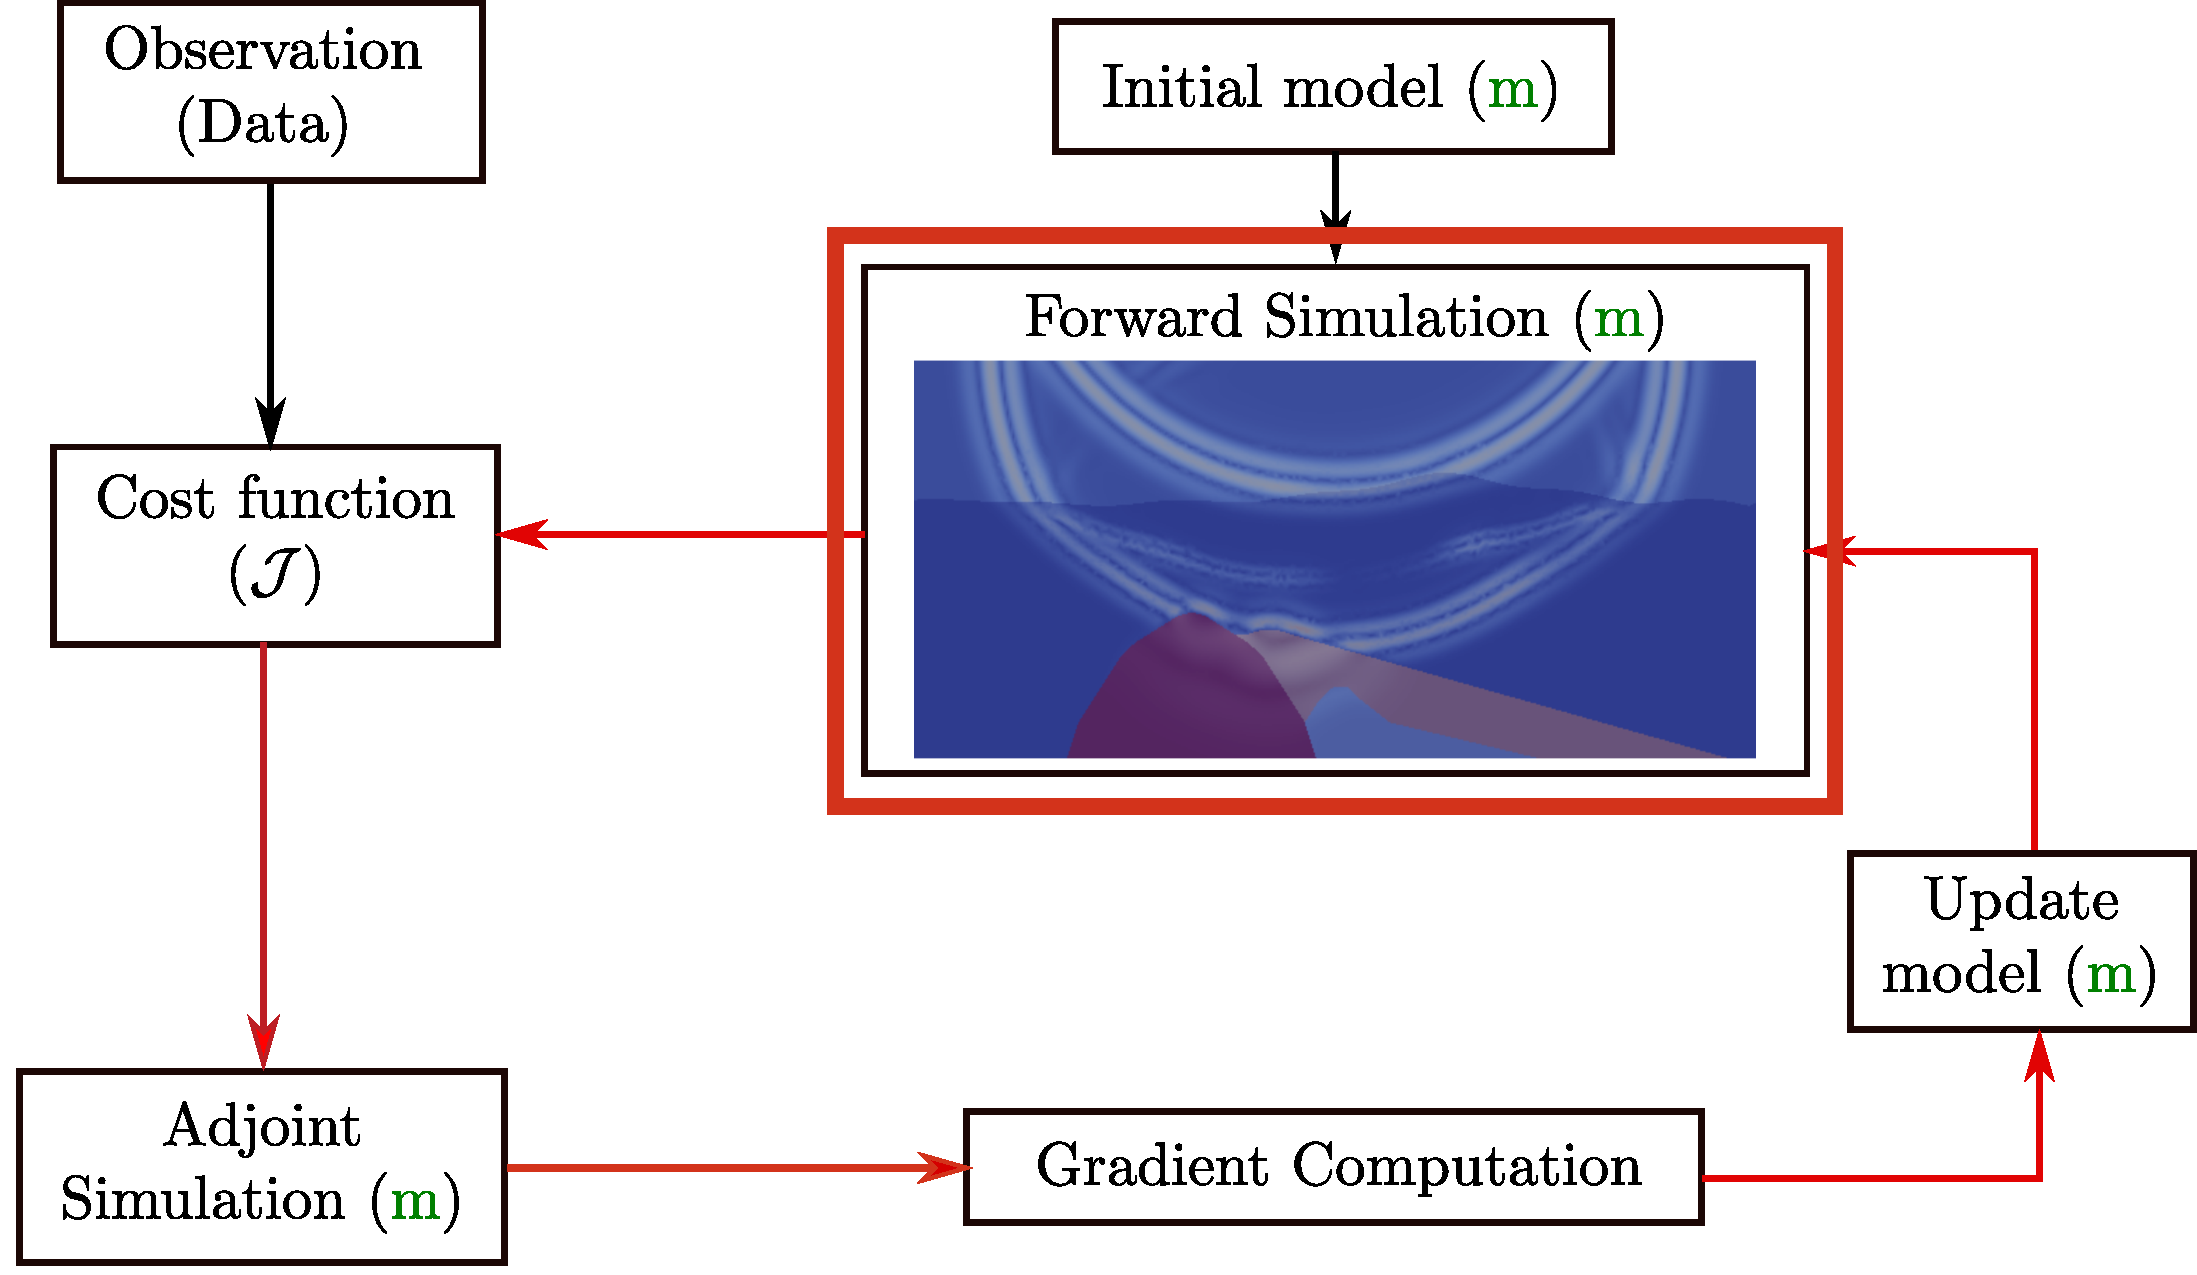
\includegraphics[scale=0.31]{image/fwi_workflow_red.pdf}
\end{figure}
\end{frame}

\begin{frame}[noframenumbering]
\begin{figure}
  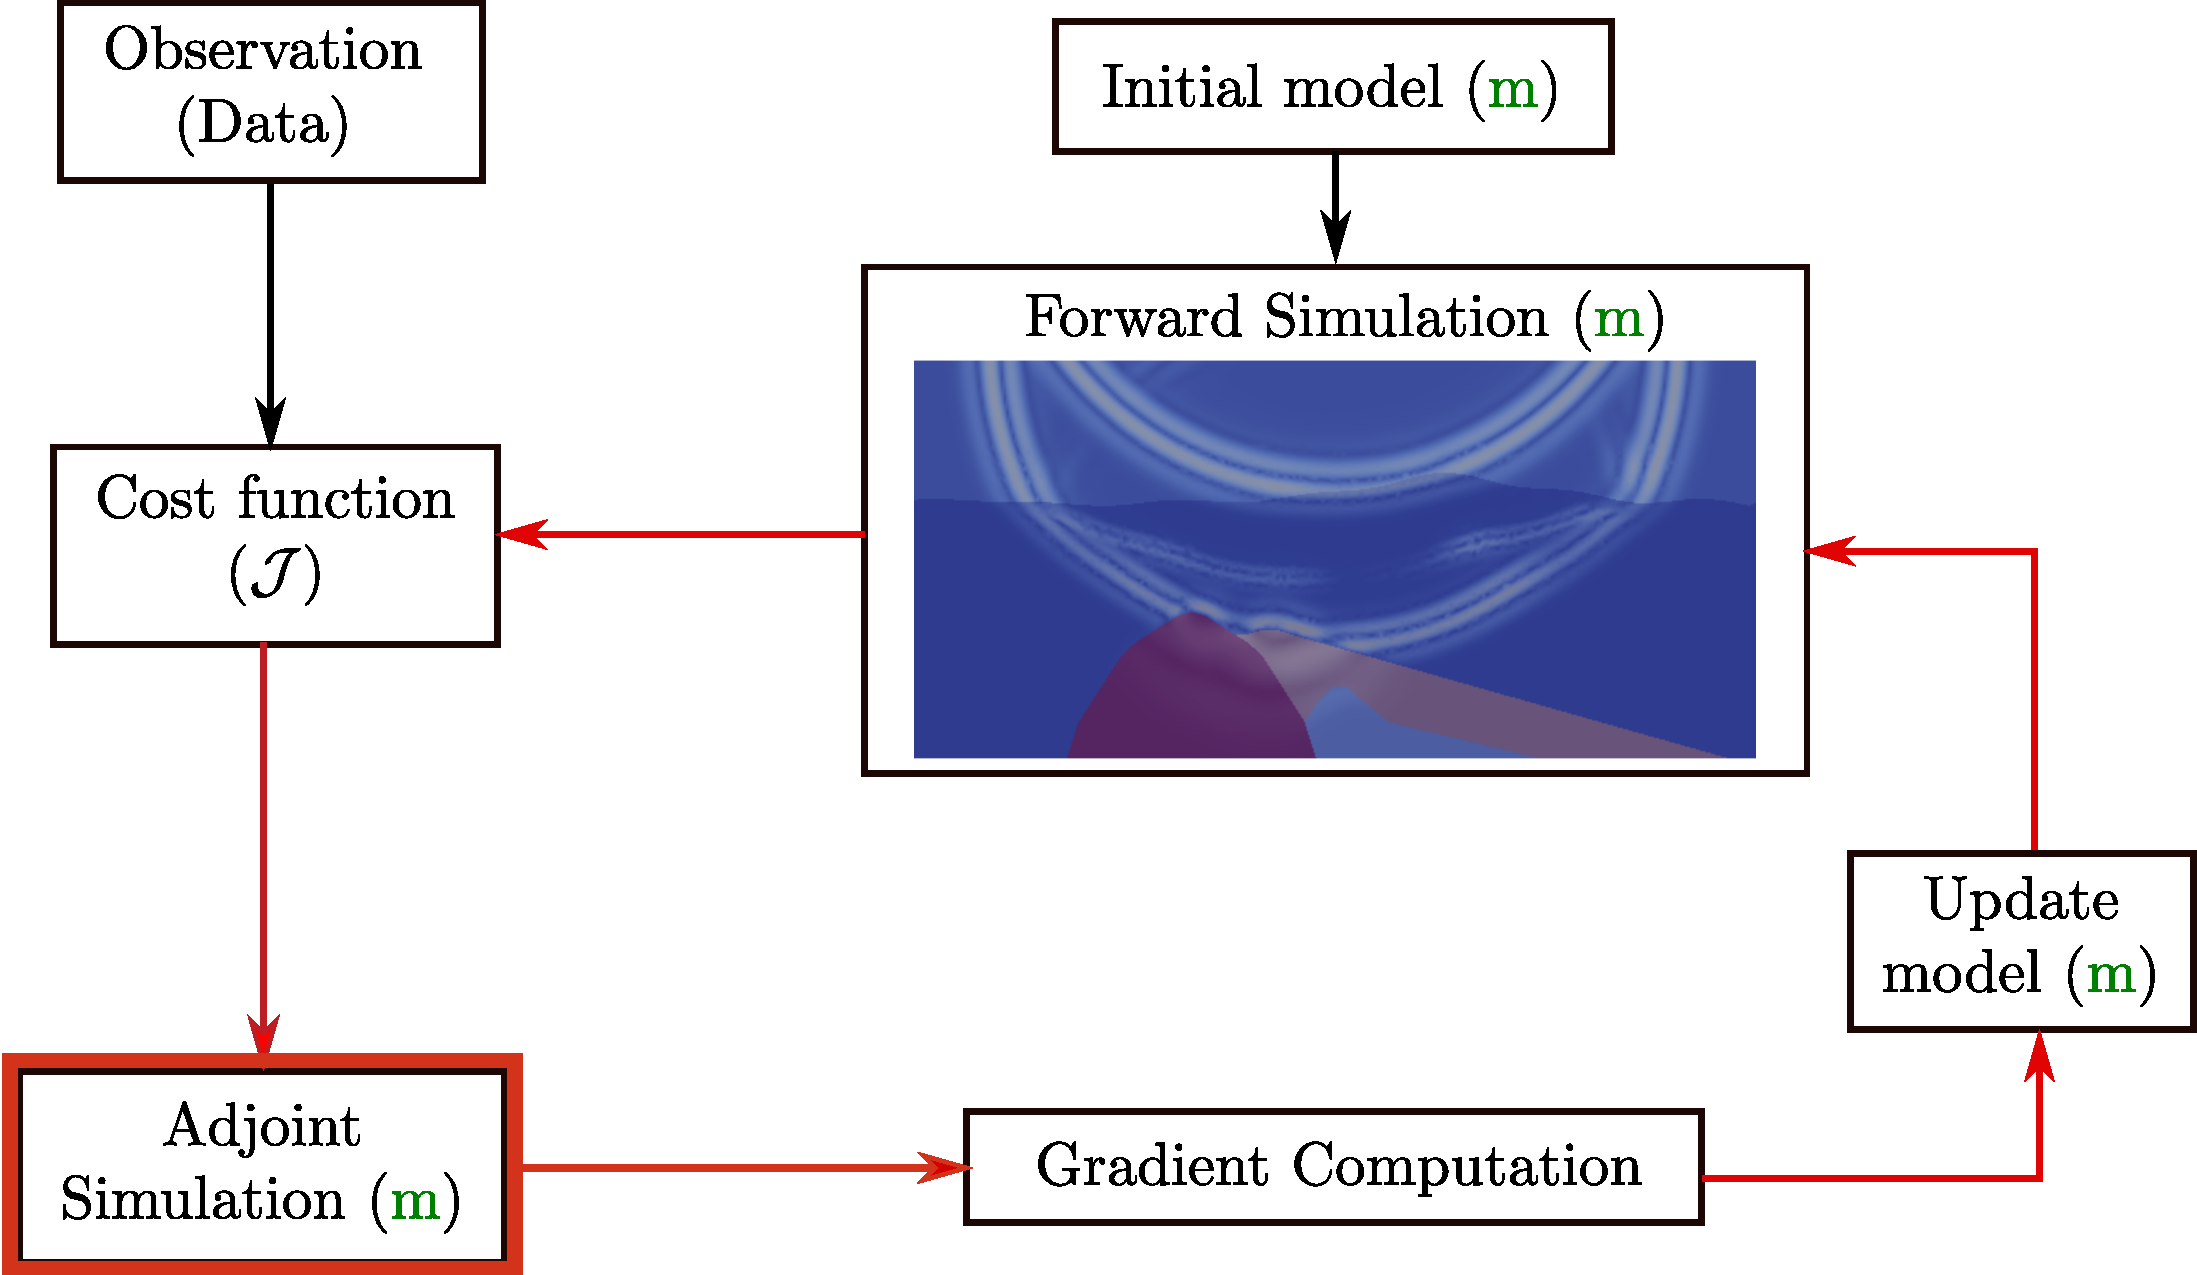
\includegraphics[scale=0.31]{image/fwi_workflow_red2.pdf}
\end{figure}
\end{frame}
     %% Pb Direct
  \section{Adjoint Studies}
\renewcommand\tikzscale{1.3}


% ============================================
% ====== Frame : Adjoint State Method  =======
% ============================================

\begin{frame}{Adjoint State Method}
\scriptsize
Lagrangian functional \footcite{plessixReviewAdjointstateMethod2006} :

  \begin{equation}
    \Lag(\qcqU,\qcqLbd,\model) = \frac{1}{2}||\textcolor{blue}{d_{obs}}-\textcolor{red}{\mathcal{R}(\qcqU)}||^2 + <\DP(\qcqU)-f_p,\qcqLbd>
  \end{equation}


  \uncover<2->{
    \begin{block}{Adjoint Equation:}
  Let us choose $\qcqLbd=\contLbd$ such as $\frac{\partial \Lag}{\partial \contU} = 0$

  \begin{equation}
 \DP^*(\contLbd) + \mathcal{R}^*(\textcolor{blue}{d_{obs}}-\mathcal{R}\contU) = 0
  \end{equation}
  \end{block}
  }

  \uncover<3->{
    \begin{block}{Gradient Expression:}
  For $\DP(\contU)-f_p = 0$ :

  \begin{equation}
    \partial_{\model_i} \CF(\model) = \partial_{\model_i} \Lag(\contU,\contLbd,\model) = \partial_{\model_i} <\DP(\contU),\contLbd>
  \end{equation}
  \end{block}
  }

\end{frame}











% ============================================
% ====== Frame : Adjoint Scheme      =========
% ============================================
\begin{frame}{Adjoint Formulation}
\begin{figure}

\definecolor{color1}{RGB}{255,174,41}   %% myOrange
%\definecolor{color2}{RGB}{216,93,99}  %% myGreen
\definecolor{color3}{RGB}{100,149,237} %% myBlue
\definecolor{color2}{RGB}{223,83,74} %% myRed

\definecolor{colorOne}{RGB}{255,174,41}   %% myOrange
%\definecolor{color2}{RGB}{216,93,99}  %% myGreen
\definecolor{colorThree}{RGB}{100,149,237} %% myBlue
\definecolor{colorTwo}{RGB}{223,83,74} %% myRed


\begin{tikzpicture}[scale=\tikzscale] %% [every node/.style={scale=1}]

\node[boxOptions]
at (0,3.5){ {\textbf{\Large\fontfamily{pzc}\selectfont Continuous \\ Direct Problem}}};

\uncover<2->{
\node[boxOptions]
at (6,3.5){ {\textbf{\Large\fontfamily{pzc}\selectfont Continuous \\ Adjoint Problem}}};

\coordinate (a) at (1.4,3.5);
\coordinate (b) at (4.7,3.5);
\draw[->, >=latex, red!50!white, line width=10pt]   (a) to node[pos=0.4,above]{\small{\textbf{\textcolor{black}{Adjoint}}}} (b) ;
}

\uncover<3->{
\node[boxOptions]
at (6,0.7){\textbf{Discretization of the Continuous Adjoint Problem}};

\draw[arrowStyleinv]
(6,2.1) to[out=90,in=90]
node[sloped,anchor=south]
{}
(6,2.6);

\coordinate (b) at (6,1.2);
\coordinate (a) at (6,3.0);
\draw[->, >=latex, red!50!white, line width=10pt]   (a) to node[fill=colorThree!0,pos=0.3]{\small{\textbf{\textcolor{black}{Discretization}}}} (b) ;
}


\uncover<4->{
\node[boxOptions]
at (0,-0.5){\textbf{Discrete \\Direct Problem}};

%% \draw[arrowStyleinv]
%% (0,0.7) to[out=90,in=90]
%% node[sloped,anchor=south]
%% {\footnotesize{Discretization ~~~~~~~~~~~~~}}
%% (0,2.5);

\coordinate (b) at (0,-0.1);
\coordinate (a) at (0,3.0);
\draw[->, >=latex, blue!50!white, line width=10pt]   (a) to node[fill=colorThree!0]{\small{\textbf{\textcolor{black}{Discretization}}}} (b) ;


\node[boxOptions]
at (6,-0.5){\textbf{Adjoint of the Discrete Problem}};


%% \draw[arrowStyle]
%% (2,0) to[out=0,in=180]
%% node[sloped,anchor=south]
%% {(*)}
%% (4,0);

\coordinate (a) at (1.4,-0.5);
\coordinate (b) at (4.7,-0.5);
\draw[->, >=latex, blue!50!white, line width=10pt]   (a) to node[pos=0.4,below]{\small{\textbf{\textcolor{black}{Adjoint}}}} (b) ;
}

\uncover<5->{
\draw[color=red,line width=2] (4.5,1.4)
rectangle (7.5,-1.0);
}
\end{tikzpicture}
\end{figure}
\end{frame}








% ============================================
% ====== Frame : Adjoint then discretize 1 ===
% ============================================

\begin{frame}{OtD : Optimize then Discretized Strategy \footcite{tarantolaInversionSeismicReflection1984}}
\scriptsize
  \begin{equation}
    \CF(\contP)=\frac{1}{2}||\textcolor{blue}{d_{obs}} - R\contP||^2
    \end{equation}

  \noindent
  \begin{multicols}{2}
    \noindent
      \begin{empheq}[left=\empheqlbrace]{align}
    & \frac{1}{\density \velocity^2}\frac{\partial \contP}{\partial t}+\nabla \cdot \contV=f_p \text{~~ on $\boldsymbol{\Omega}$}\\
    & \density\frac{\partial \contV}{\partial t}+\nabla\contP=0  \text{~~ on $\boldsymbol{\Omega}$}\\
    & \contP=0 \text{~~ on $\textcolor{\myred}{\boldsymbol{\Gamma_1}}$} \\
    & \contP-\velocity \density \contV \cdot \normal=0 \text{~~ on $\textcolor{\myblue}{\boldsymbol{\Gamma_2}}$}\\
    & \contP(0) = 0 \text{, ~~~} \contV(0) = 0
      \end{empheq}
\vfill
    \columnbreak
    \noindent
    \uncover<2->{
      \vspace{-0.5cm}
      \begin{empheq}[left=\empheqlbrace]{align}
    & \hspace{0.2cm} \frac{1}{\density \velocity^2}\frac{\partial \Lbdun}{\partial t}+\nabla \cdot \Lbdeux=R^*(R\contP - \textcolor{blue}{d_{obs}})(\Tfinal -t)\\
    &  \hspace{0.2cm} \density\frac{\partial \Lbdeux}{\partial t}+\nabla\Lbdun=0  \text{~~ on $\boldsymbol{\Omega}$}\\
    &  \hspace{0.2cm} \Lbdun=0 \text{~~ on $\textcolor{\myred}{\boldsymbol{\Gamma_1}}$} \\
    &  \hspace{0.2cm}  \Lbdun - \velocity \density \Lbdeux \cdot \normal=0 \text{~~ on $\textcolor{\myblue}{\boldsymbol{\Gamma_2}}$}\\
    &  \hspace{0.2cm} \Lbdun(T) = 0 \text{, ~~~} \Lbdeux(T) = 0
      \end{empheq}
      \vfill
      }
  \end{multicols}
  \vspace{-0.5cm}
  \begin{equation}
    t\in[0,T] \uncover<2->{\text{~~~~~~~~~~~~~~~~~~~~~~~~~~} t\in[T,0]}
  \end{equation}

\end{frame}



% ============================================
% ====== Frame : Adjoint then discretize 1 ===
% ============================================

\begin{frame}[noframenumbering]{OtD : Optimize then Discretized Strategy}
\scriptsize
  \begin{equation}
    \CF(\contP)=\frac{1}{2}||\textcolor{blue}{d_{obs}} - R\contP||^2
    \end{equation}

  \noindent
  \begin{multicols}{2}
    \noindent
      \begin{empheq}[left=\empheqlbrace]{align}
    & \frac{1}{\density \velocity^2}\frac{\partial \contP}{\partial t}+\nabla \cdot \contV=f_p \text{~~ on $\boldsymbol{\Omega}$}\\
    & \density\frac{\partial \contV}{\partial t}+\nabla\contP=0  \text{~~ on $\boldsymbol{\Omega}$}\\
    & \contP=0 \text{~~ on $\textcolor{\myred}{\boldsymbol{\Gamma_1}}$} \\
    & \contP-\velocity \density \contV \cdot \normal=0 \text{~~ on $\textcolor{\myblue}{\boldsymbol{\Gamma_2}}$}\\
    & \contP(0) = 0 \text{, ~~~} \contV(0) = 0
      \end{empheq}
\vfill
    \columnbreak
    \noindent
    \uncover<1->{
            \vspace{-0.5cm}
      \begin{empheq}[left=\empheqlbrace]{align}
    & \hspace{0.2cm} \frac{1}{\density \velocity^2}\frac{\partial \Lbdun}{\partial t}+\nabla \cdot \Lbdeux=R^*(R\contP - \textcolor{blue}{d_{obs}})(\Tfinal -t)\\
    &  \hspace{0.2cm} \density\frac{\partial \Lbdeux}{\partial t}+\nabla\Lbdun=0  \text{~~ on $\boldsymbol{\Omega}$}\\
    &  \hspace{0.2cm} \Lbdun=0 \text{~~ on $\textcolor{\myred}{\boldsymbol{\Gamma_1}}$} \\
    &  \hspace{0.2cm}  \Lbdun - \velocity \density \Lbdeux \cdot \normal=0 \text{~~ on $\textcolor{\myblue}{\boldsymbol{\Gamma_2}}$}\\
    &  \hspace{0.2cm} \Lbdun(T) = 0 \text{, ~~~} \Lbdeux(T) = 0
      \end{empheq}
      \vfill
      }
  \end{multicols}
  \vspace{-0.5cm}
  \begin{equation}
    t\in[0,T] \uncover<1->{\text{~~~~~~~~~~~~~~~~~~~~~~~~~~} t\in[T,0]}
  \end{equation}

  \uncover<1->{
\begin{block}{NB:}
  Having self-adjoint continuous problem enables to use the same discretization routines to simulate the forward and the adjoint state.
\end{block}
}
\end{frame}




\subsection{Discretize then Adjoint}

% ============================================
% ====== Frame : Discretize then Adjoint 1 ===
% ============================================
\begin{frame}{DtO : Discretize then Optimize Strategy}{Example With RK2}

  For any time-schemes we get :
  \begin{equation}
    \textcolor{\myblue}{\boldsymbol{L}}\discreteU=\textcolor{\myblue}{\boldsymbol{E}}\discreteF
  \end{equation}

  \uncover<2->{
  \small
      For instance wuth RK2 time-scheme we get:
    \begin{equation}
      \discreteU^{n+1}=B\discreteU^n+\textcolor{\myblue}{\boldsymbol{C_0}}\discreteF^n+\textcolor{\myblue}{\boldsymbol{C_{\frac{1}{2}}}}\discreteF^{n+\frac{1}{2}}
    \end{equation}
    }


  \uncover<3->{
\begin{equation}
  \textcolor{\myblue}{\boldsymbol{L}}\discreteU=\textcolor{\myblue}{\boldsymbol{E}}\discreteF=\discreteG
\end{equation}
\begin{equation}
  \begin{pmatrix}
    I & & & & \\
    -B&I & & & \\
    & -B&I  & & \\
    & & \ddots & \ddots   & \\
    & &  & -B &I \\
    %% \vdots & \ddots & \vdots \\
    %% 0      & \cdots & 1
  \end{pmatrix}
    \begin{pmatrix}
    \discreteU^0 \\
    \discreteU^1 \\
    \discreteU^2 \\
    \vdots \\
    \discreteU^n \\
  \end{pmatrix}=
  \begin{pmatrix}
    \discreteG^0 \\
    \discreteG^1 \\
    \discreteG^2 \\
    \vdots \\
    \discreteG^n \\
  \end{pmatrix}
\end{equation}
}
\end{frame}



% ============================================
% ====== Frame : Discretize then Adjoint 2 ===
% ============================================
\begin{frame}[noframenumbering]{DtO : Discretize then Optimize Strategy}

   For any time-schemes we get:
    \begin{equation}
      \textcolor{\myblue}{\boldsymbol{L}}\discreteU=\textcolor{\myblue}{\boldsymbol{E}}\discreteF \uncover<1->{=\discreteG}
    \end{equation}

    We are looking for a Discrete Adjoint state satisfying :
    \begin{equation}
      \textcolor{\myblue}{\boldsymbol{L^*}}\discreteLbd=-R^*(\textcolor{blue}{d_{obs}}-R\discreteU) \uncover<1->{=\discreteD}
    \end{equation}

    \uncover<2->{
    \begin{block}{Adjoint test}
    With the adjoint operator $\textcolor{\myblue}{\boldsymbol{L^*}}$ satisfying :
      \begin{equation}
    <\textcolor{\myblue}{\boldsymbol{L}}\discreteU,\discreteLbd>=<\discreteU,\textcolor{\myblue}{\boldsymbol{L^*}}\discreteLbd>
      \end{equation}
        \begin{equation}
        <\discreteG,\discreteLbd>=<\discreteU,\discreteD> \text{~~~(Adjoint Test)}
      \end{equation}


      \begin{center}
        Adjoint test succeeds $\Longleftrightarrow$  operator $\textcolor{\myblue}{\boldsymbol{L^*}}$  well established
      \end{center}
    \end{block}
    }

\end{frame}



\begin{frame}{Discretize then Optimize}

  $\textcolor{\myblue}{\boldsymbol{L^*}}$ is challenging to develop:

  \begin{itemize}
  \item<2-> Requires the adjoint operator of the fluxes \footcite{wilcoxDiscretelyExactDerivatives2013} (Reverse all the communications).
  \item<3-> Requires the development of the adjoint operator for all propagator.
  \item<4-> Architectures of the program divided into several libraries.
    \begin{itemize}
    \item<5-> Requires the development of the adjoint in each inner functions.
    \item<6-> Prevents the use of automatic differentiation tools \footcite{griewank2008evaluating}.
    \end{itemize}
  \end{itemize}

\end{frame}







% ================================================
% ====== Frame : Adjoint Strategies Comparison ===
% ================================================

\begin{frame}{Adjoint Strategies Comparison}
  \begin{columns}
    \begin{column}[t]{0.5\textwidth}
      \textbf{\textcolor{red}{Optimize Then Discretize}}
      \vspace{0.5cm}
%      \dotfill % to show column margins
      \begin{itemize}
      \item[\textcolor{\mygreen}{\textbf{+}}] Physical approach
      \item[\textcolor{\mygreen}{\textbf{+}}] Same discrete operators for Forward and Backward
      \item[\textbf{- -}] Approximate gradient \footnotemark
      \end{itemize}
      %      \dotfill
      \vspace{0.5cm}
    \end{column}\vrule \hfill
    \begin{column}[t]{0.5\textwidth}
      \uncover<2->{
      \textbf{\textcolor{blue}{Discretize then Optimize}}
      \vspace{0.5cm}
%            \dotfill
      \begin{itemize}
      \item[\textcolor{\mygreen}{\textbf{+}}] Numerical approach
      \item[\textcolor{\mygreen}{\textbf{+}}] Has an Adjoint Test
      \item[\textcolor{\mygreen}{\textbf{+}}] Exact Gradient
      \item[\textbf{-}] Not that obvious to develop
      \item[\textcolor{black}{\textbullet}] Possible inconsistency of the adjoint scheme \footnotemark
      \end{itemize}
      }
    \end{column}
  \end{columns}
  \addtocounter{footnote}{-1}
  \footcitetext{gunzburger2002perspectives}
  \addtocounter{footnote}{+1}
  \footcitetext{sei1995note}
\end{frame}


% ================================================
% ====== Frame : 1D comparison ===================
% ================================================



\subsection{1D FWI problem}
\begin{frame}{1D FWI problem}

\begin{figure}[H]
  \centering
   \begin{tikzpicture}[scale=1.5]
      \draw[color=black,line width=2.1](0.0,0.0) -- (6.5,0);
      %\draw[color=blue, line width=10] (0,-0.02) node {$\bullet$} ;
      %\draw[color=blue, line width=10] (5,-0.02) node {$\bullet$} ;
     % \draw node[color=blue,fill,circle,minimum size=0.01](1,1) {};
      \node[anchor=south east, color=black]
      at (0,0) {};
      %\node[anchor=south west, color=black]
      %at (4.0,0.2) {\Large $\velocity$ ?};

      \pgfmathsetmacro{\x}{0.0}
      \draw[color=black,line width=2.1](\x,0.1) -- (\x,-0.1);

      \pgfmathsetmacro{\x}{6.5}
      \draw[color=black,line width=2.1](\x,0.1) -- (\x,-0.1);

      \pgfmathsetmacro{\x}{0.5}
      \draw[color=black,line width=1.5](\x,0.1) -- (\x,-0.1);
      \draw[color=black,line width=1.5](\x,0.1) -- (\x,-0.1);



      \pgfmathsetmacro{\x}{1.0}
      \draw[color=black,line width=1.5](\x,0.1) -- (\x,-0.1);
      \pgfmathsetmacro{\x}{1.5}

      \draw[color=black,line width=1.5](\x,0.1) -- (\x,-0.1);
      \pgfmathsetmacro{\x}{2.0}
      \draw[color=black,line width=1.5](\x,0.1) -- (\x,-0.1);
      \pgfmathsetmacro{\x}{2.5}
      \draw[color=black,line width=1.5](\x,0.1) -- (\x,-0.1);
      \pgfmathsetmacro{\x}{3.0}
      \draw[color=black,line width=1.5](\x,0.1) -- (\x,-0.1);
      \pgfmathsetmacro{\x}{3.5}
      \draw[color=black,line width=1.5](\x,0.1) -- (\x,-0.1);
      \pgfmathsetmacro{\x}{4.0}
      \draw[color=black,line width=1.5](\x,0.1) -- (\x,-0.1);
      \pgfmathsetmacro{\x}{4.5}
      \draw[color=black,line width=1.5](\x,0.1) -- (\x,-0.1);
            \pgfmathsetmacro{\x}{5.0}
      \draw[color=black,line width=1.5](\x,0.1) -- (\x,-0.1);

            \pgfmathsetmacro{\x}{5.5}
      \draw[color=black,line width=1.5](\x,0.1) -- (\x,-0.1);


            \pgfmathsetmacro{\x}{6.0}
      \draw[color=black,line width=1.5](\x,0.1) -- (\x,-0.1);

      \pgfmathsetmacro{\x}{1.8}
      \pgfmathsetmacro{\dx}{0.2}
      \pgfmathsetmacro{\y}{-0.2}
      \pgfmathsetmacro{\dy}{-0.4}
      \node (A) at (\x,\y) {}; % B = 5
      \node (B) at (\x+\dx,\y+\dy) {}; % AC = 3
      \node (C) at (\x-\dx,\y+\dy) {}; % BC = 4
      \node (receiver) at (\x,\y+\dy-0.1) {Receiver}; % BC = 4
     % \draw (A) -- (B) -- (C) -- (A);
      \begin{scope}%[on background layer]
        \fill [blue] (A.center) -- (B.center) -- (C.center) -- cycle;
      \end{scope}

            \pgfmathsetmacro{\x}{0.6}
      \pgfmathsetmacro{\dx}{0.2}
      \pgfmathsetmacro{\y}{-0.2}
      \pgfmathsetmacro{\dy}{-0.4}
      \node (A) at (\x,\y) {}; % B = 5
      \node (B) at (\x+\dx,\y+\dy) {}; % AC = 3
      \node (C) at (\x-\dx,\y+\dy) {}; % BC = 4
      \node (source) at (\x,\y+\dy-0.1) {Source}; % BC = 4
      %\draw [red] (A) -- (B) -- (C) -- (A);
      \begin{scope}%[on background layer]
        \fill [red] (A.center) -- (B.center) -- (C.center) -- cycle;
      \end{scope}
\end{tikzpicture}

  \caption*{1D domain $\Domain$.}
  \label{1D_domain}
\end{figure}


\uncover<2->{
      \setlength{\plotwidth} {3.5cm}
      \setlength{\plotheight}{2.8cm}
      \pgfplotsset{every tick label/.append style={font=\tiny}}
      \begin{figure}[H]
      \begin{subfigure}{0.45\textwidth}
        \centering
          \begin{tikzpicture}
      \begin{axis}[%
          width=\plotwidth, height=\plotheight,,
          at={(0,0)},scale only axis,separate axis lines,xminorticks=true,
          xlabel={\scriptsize{$x$}},
          ylabel={\scriptsize{Wavespeed (m.s$^{-1}$)}},
          %ylabel={$\velocity$},
          %%   ymode=log,
          yminorticks=true,
          %xmin=0.,xmax=100.,
          ymin=900,ymax=1300
        ]

        %% load current data
        %% -----------------
        \addplot[color=blue!50!black,mark options={solid},
          forget plot,line width=1pt,
          mark size=2pt]
        table[x=monx,y=mony]
        {graph/VP0.dat};
        %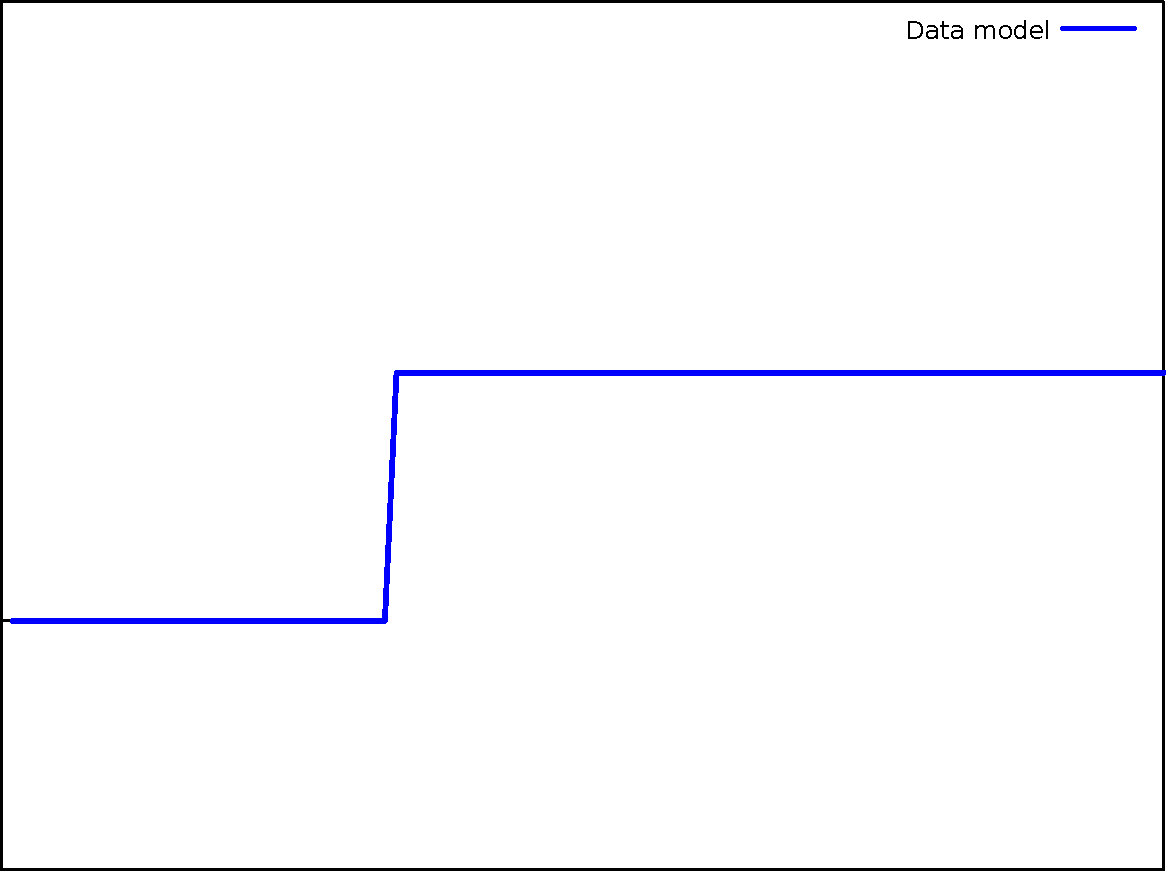
\includegraphics{images/data_bis.pdf}
      \end{axis}
      %% --------------------------------------------------------------------
          \end{tikzpicture}
          \caption*{Initial wavespeed model.}
          \label{1D_initial}
      \end{subfigure}
     \begin{subfigure}{0.45\textwidth}
        \centering
          \begin{tikzpicture}
      \begin{axis}[%
          width=\plotwidth, height=\plotheight,,
          at={(0,0)},scale only axis,separate axis lines,xminorticks=true,
          xlabel={\scriptsize{$x$}},
          %ylabel={$\velocity$},
          %%   ymode=log,
          yminorticks=true,
          ymin=900,ymax=1300
          %%   xmin=0.,xmax=100.
        ]

        %% load current data
        %% -----------------
        \addplot[color=blue!50!black,mark options={solid},
          forget plot,line width=1pt,
          mark size=2pt]
        table[x=monx,y=mony]
        {graph/VP100.dat};
      \end{axis}
      %% --------------------------------------------------------------------
          \end{tikzpicture}
          \caption*{Target wavespeed model.}
          \label{1D_target}
     \end{subfigure}
     \label{model_1D_target}
      \end{figure}
      }

\end{frame}


\begin{frame}{1D FWI problem}{Gradient validation}

  \setlength{\plotwidth}{6.0cm}
\setlength{\plotheight}{4.5cm}
   \begin{figure}
     \centering
         \begin{tikzpicture}
      \begin{axis}[%
          width=\plotwidth, height=\plotheight,,
          at={(0,0)},scale only axis,separate axis lines,xminorticks=true,
          xlabel={\scriptsize{$x$}},
          ylabel={\scriptsize{Gradient amplitude}},
          legend pos=south east
        ]
        %% load current data
        %% -----------------
        \addplot[color=black!50!black,mark options={solid}, mark = triangle,
          line width=1pt,
          mark size=0pt]
        table[x=monx,y=mony]
        {graph/grad_df.dat};
        \addlegendentry{\scriptsize{FD gradient}}

        \addplot[color=blue!50!black,mark options={solid}, mark = triangle,
          line width=1pt,
          mark size=0pt]
        table[x=monx,y=mony]
        {graph/grad_dto.dat};
        \addlegendentry{\scriptsize{DtO gradient}}


        \addplot[color=red!50!black,mark options={solid}, mark = triangle,
          line width=1pt,
          mark size=0pt]
        table[x=monx,y=mony]
        {graph/grad_otd.dat};
        \addlegendentry{\scriptsize{OtD gradient}}




        %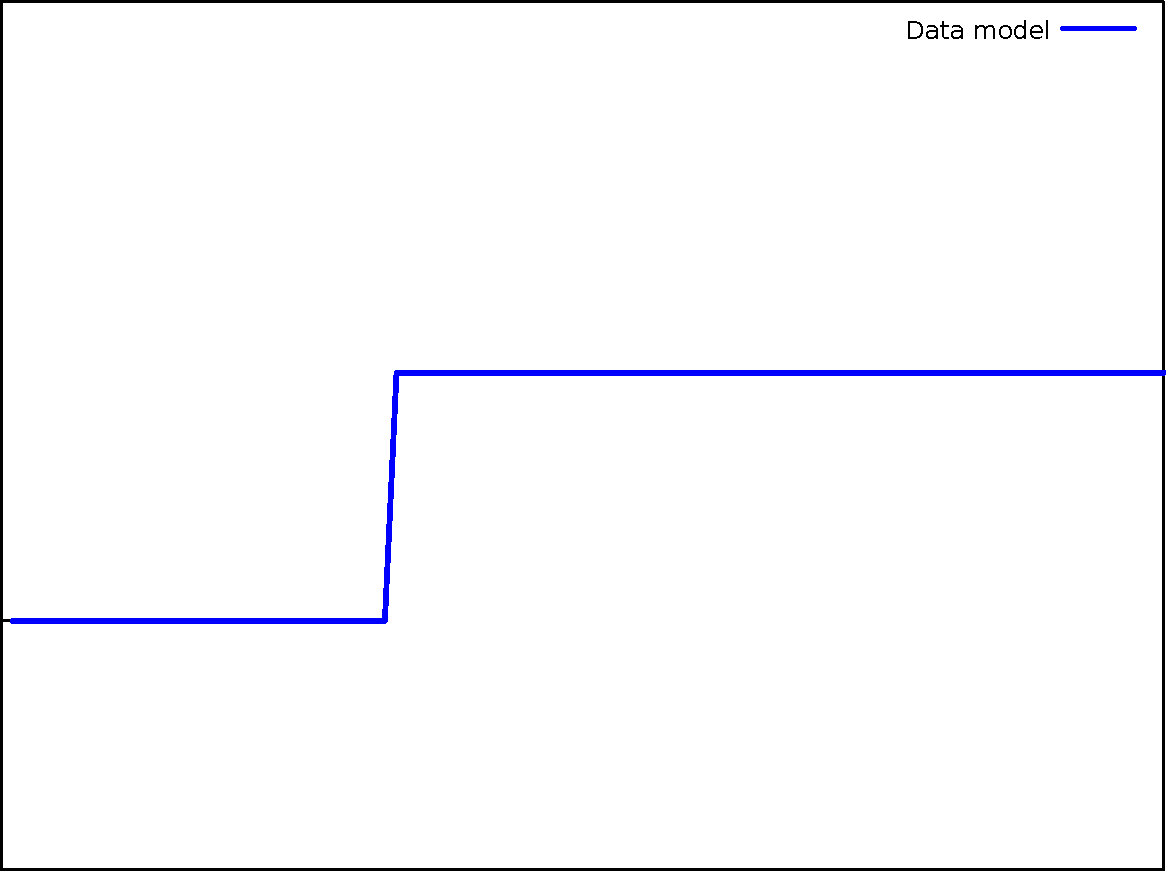
\includegraphics{images/data_bis.pdf}
      \end{axis}
      %% --------------------------------------------------------------------
         \end{tikzpicture}
     \end{figure}

\end{frame}


\begin{frame}{1D Results with L-BFGS}
        \pgfplotsset{every tick label/.append style={font=\tiny}}
      \setlength{\plotwidth} {4.5cm}
      \setlength{\plotheight}{3.0cm}
      \begin{figure}[!htbp]
        \begin{subfigure}{0.45\textwidth}
          \hspace{-0.5cm}
          \vspace{0.2cm}
        \centering
           \begin{tikzpicture}
      \begin{axis}[%
          width=\plotwidth, height=\plotheight,,
          at={(0,0)},scale only axis,separate axis lines,xminorticks=true,
          xlabel={\scriptsize{$x$}},
          ylabel={$\velocity$},
          %%   ymode=log,
          yminorticks=true,
          ymin=900,ymax=1300,
          legend pos=south east
          %%   xmin=0.,xmax=100.
        ]

        %% load current data
        %% -----------------
          \addplot[color=blue!50!black,mark options={solid}, mark = triangle,
          line width=1pt,
          mark size=1pt]
        table[x=monx,y=mony]
        {graph/vp_DTO.dat};
       \addlegendentry{DtO}

         \addplot[color=red!50!black,mark options={solid}, mark = *,
          line width=1pt,
          mark size=1pt]
        table[x=monx,y=mony]
        {graph/vp_OTD.dat};
        \addlegendentry{OtD}

      \end{axis}
      %% --------------------------------------------------------------------
          \end{tikzpicture}
           \caption*{\small{Final 1D wavespeed model reconstructed}.}
           \label{vp_DTO_vs_OTD}
      \end{subfigure}
      \begin{subfigure}{0.45\textwidth}
        \centering
          \begin{tikzpicture}
      \begin{axis}[%
          width=\plotwidth, height=\plotheight,,
          at={(0,0)},scale only axis,separate axis lines,xminorticks=true,
          xlabel={\scriptsize{iteration}},
          ylabel={$\CF$},
          ymode=log,
          yminorticks=true,
          %ymin=900,ymax=1300,
          legend pos=north east
          %%   xmin=0.,xmax=100.
        ]

        %% load current data
        %% -----------------
          \addplot[color=blue!50!black,mark options={solid}, mark = triangle,
          line width=1pt,
          mark size=1pt]
        table[x=monx,y=mony]
        {graph/run_lbfgs_DTO.dat};
       \addlegendentry{DtO}

         \addplot[color=red!50!black,mark options={solid}, mark = *,
          line width=1pt,
          mark size=1pt]
        table[x=monx,y=mony]
        {graph/run_lbfgs_OTD.dat};
        \addlegendentry{OtD}

      \end{axis}
      %% --------------------------------------------------------------------
          \end{tikzpicture}
          \caption*{\small{Cost function evolution through 400 L-BFGS iterations.}}
          \label{cf_DTO_vs_OTD}
         \end{subfigure}
         \end{figure}

\end{frame}


\begin{frame}
\begin{figure}
  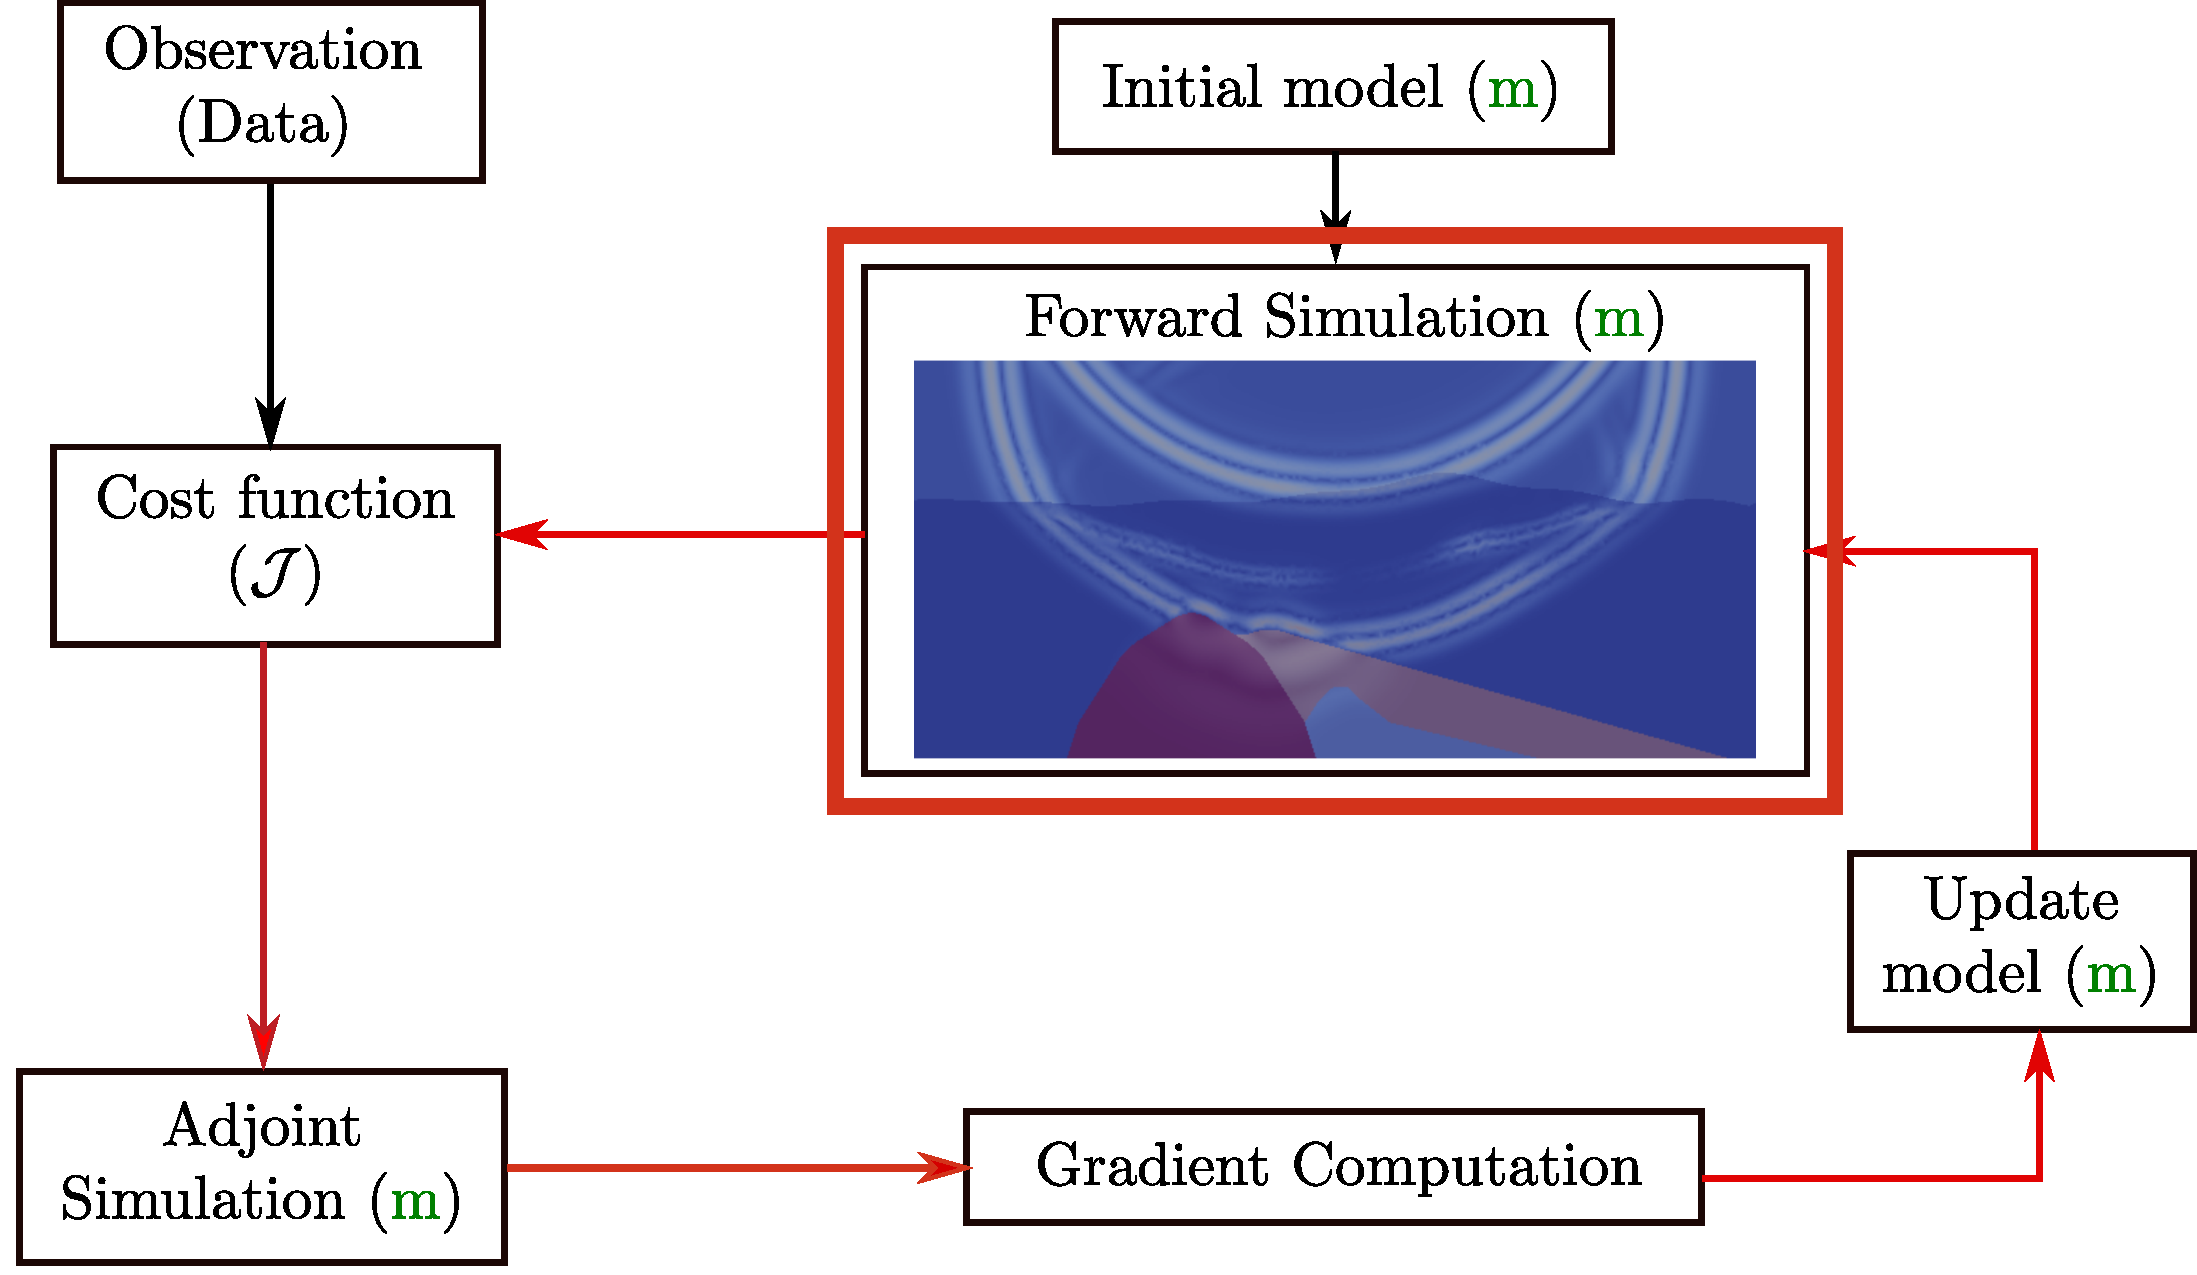
\includegraphics[scale=0.31]{image/fwi_workflow_red.pdf}
\end{figure}
\end{frame}

\begin{frame}[noframenumbering]
\begin{figure}
  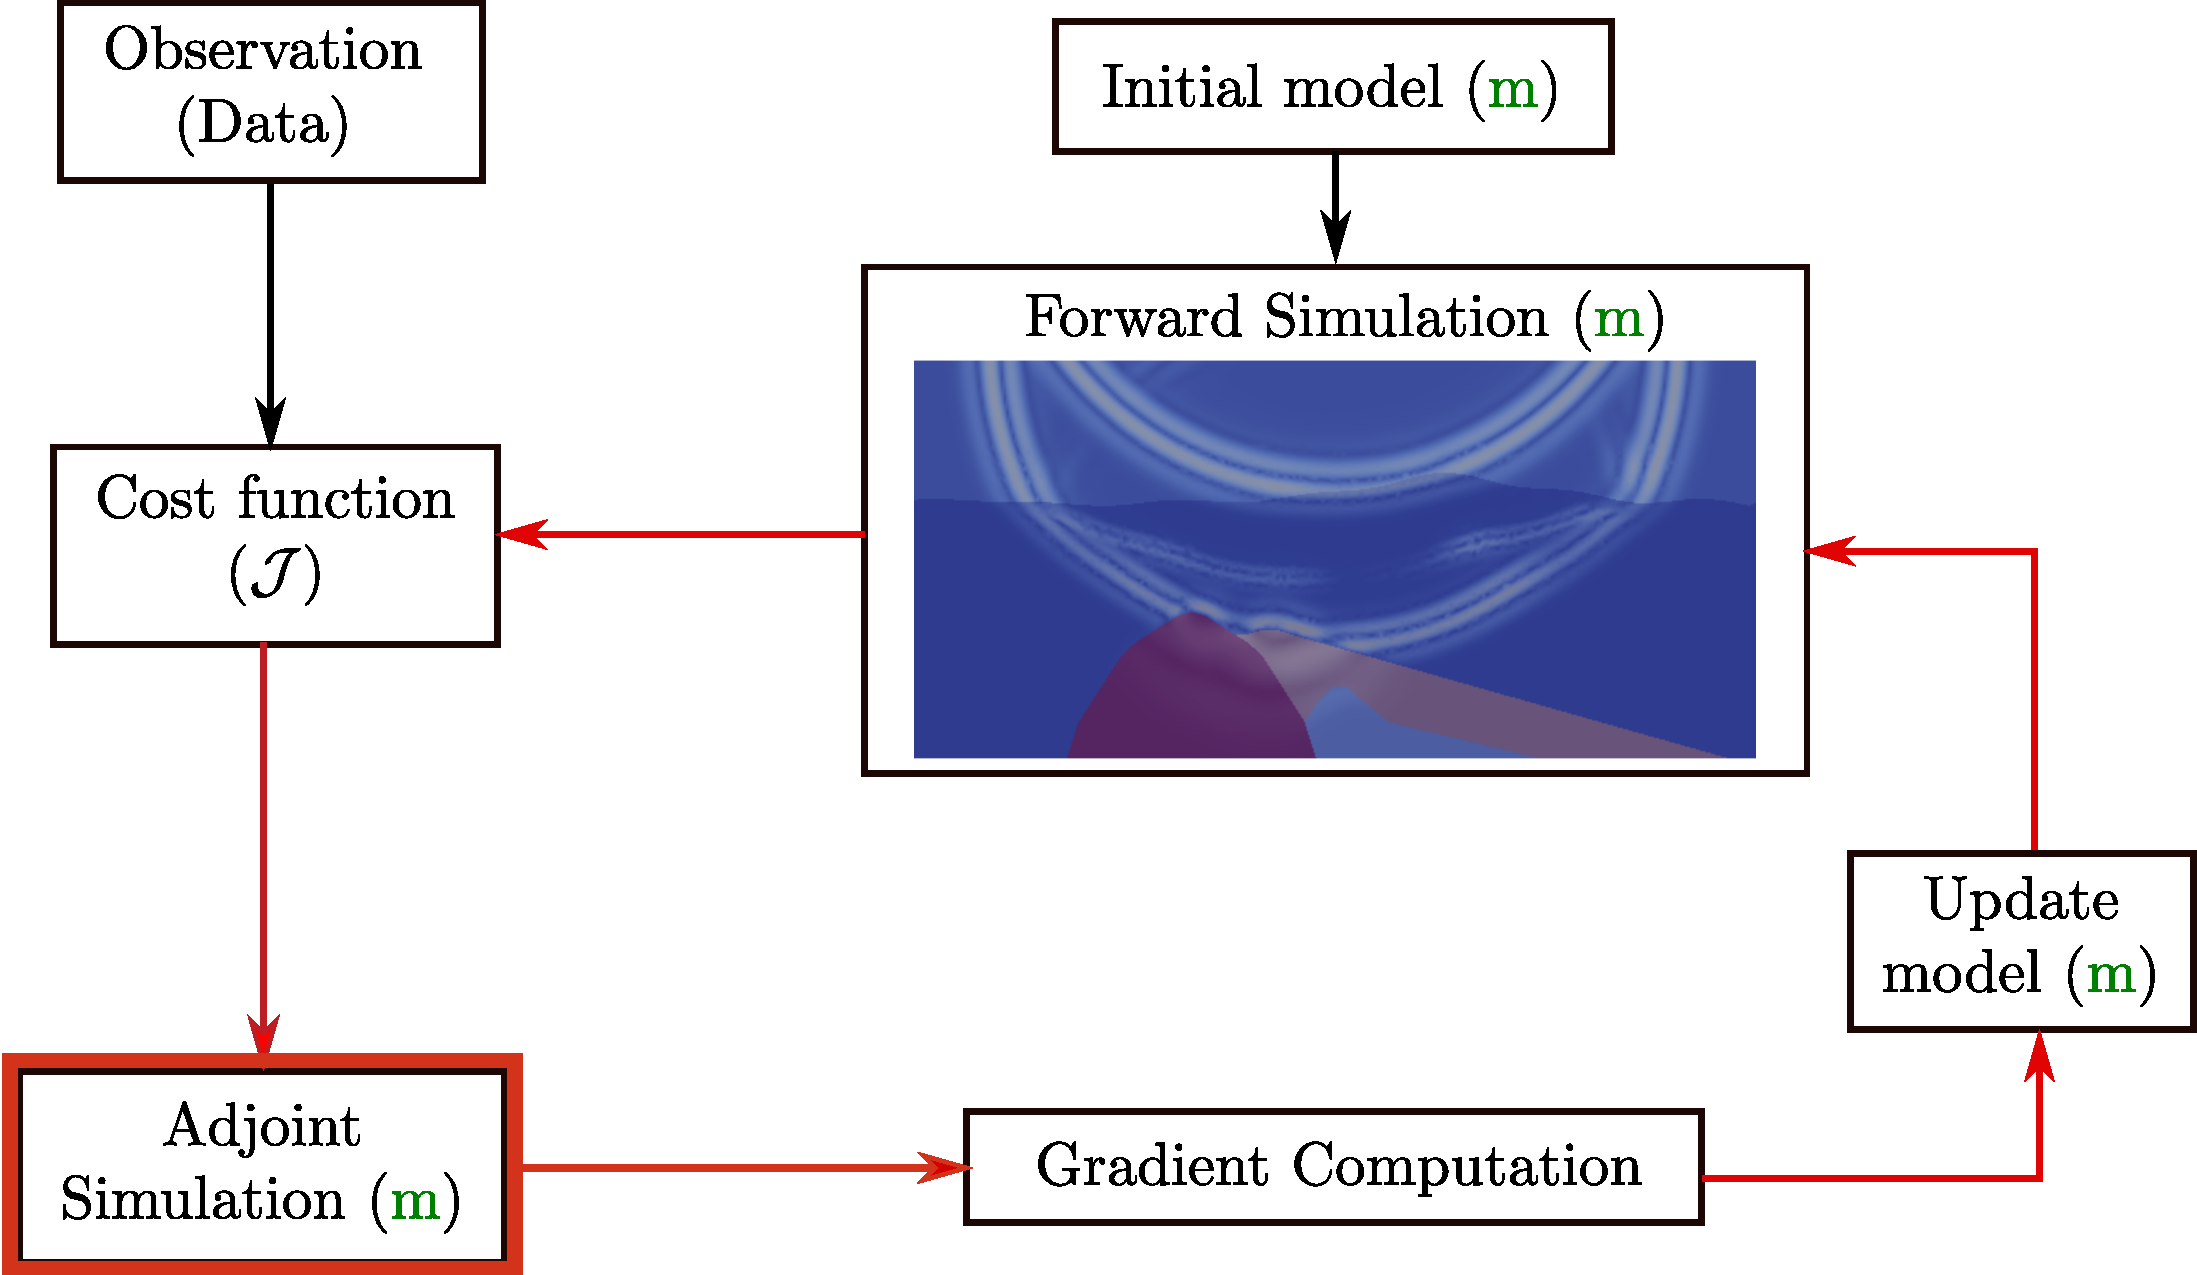
\includegraphics[scale=0.31]{image/fwi_workflow_red2.pdf}
\end{figure}
\end{frame}

\begin{frame}[noframenumbering]
\begin{figure}
  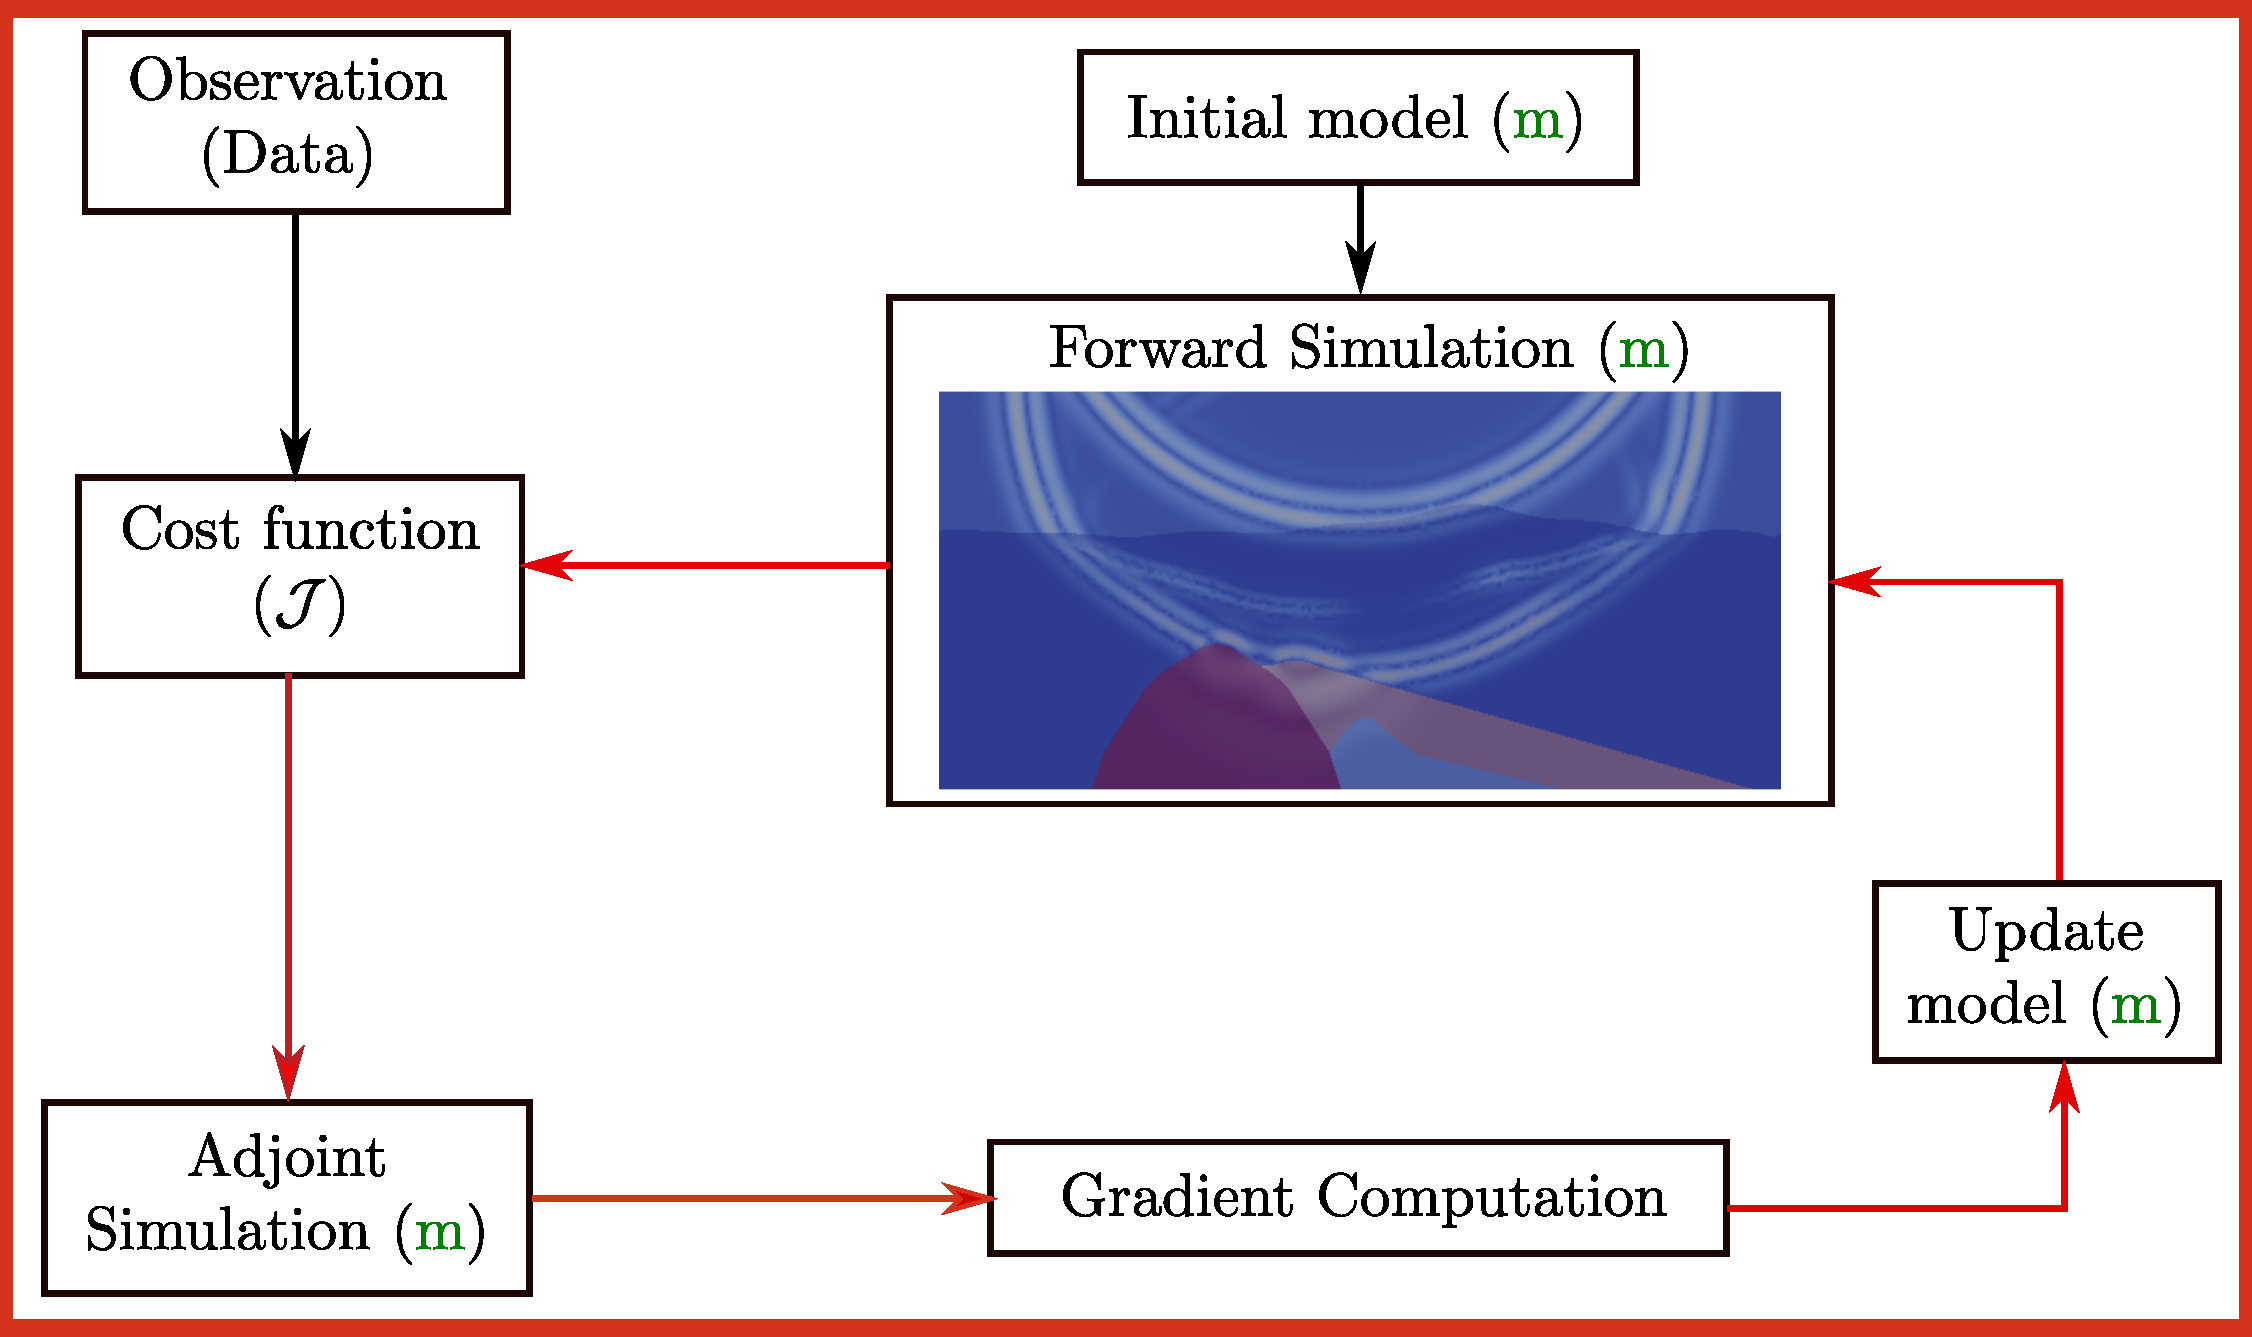
\includegraphics[scale=0.31]{image/fwi_workflow_all.pdf}
\end{figure}
\end{frame}








% ==========================================================
% ====== Frame : Choix et gradient expression ==============
% ==========================================================

%% \begin{frame}{Conclusion concerning the gradient expression}
%%   We chose the \textbf{Optimize then Discretize} strategy.


%%   \begin{overprint}
%%     \onslide<2>
%% \begin{block}{Gradient expression on the $l^{th}$ parameter for constant parametrization par element ($\frac{1}{\bm}{\density}$).}
%%   \begin{align}
%% (\frac{\partial}{\partial \frac{1}{\bm}_l} \CF(\smodel))_h  &\approx \deltat \detJKl \sum_{n=0}^\nt  (\frac{\partial}{\partial t} {{\boldsymbol{\textcolor{\myred}{\scoefPolP}}^n)}^{\element^l}}^\top \MassRef  {(\boldsymbol{\textcolor{\myred}{\scoefAdjP}}^n)}^{\element^l}\,,
%% \end{align}
%% and
%% \begin{align}
%% (\frac{\partial}{\partial \density_l} \CF(\smodel))_h  &\approx \deltat \detJKl \sum_{d=1}^\dim \sum_{n=0}^\nt  (\frac{\partial}{\partial t} {{\boldsymbol{\textcolor{\myred}{\scoefPolVd}}^n)}^{\element^l}}^\top \MassRef  {(\boldsymbol{\textcolor{\myred}{\scoefAdjVd}}^n)}^{\element^l} \,.
%% \end{align}
%% \end{block}

%% \onslide<3>
%% \vspace{-0.3cm}
%% \begin{block}{Gradient expression for \textbf{WADG} parametrization for the the $q^{th}$ quadrature point on the $l^{th}$ element ($\frac{1}{\bm}{\density}$).}
%%   \begin{align}
%% \left(\frac{\partial}{\partial \frac{1}{\bm}_{l,q}} \CF(\smodel)\right)_h \approx  \deltat \detJKl \sum_{n=0}^\nt  {{\textcolor{\myred}{\coefPolP}^n}^{\element^l}}^\top \Pquad  diag(\weight \boldsymbol{\delta_q}) \Pquad^\top   {\textcolor{\myred}{\coefAdjP}^n}^{\element^l} \,,
%% \end{align}
%% and
%% \begin{align}
%% \left(\frac{\partial}{\partial \density_{l,q}} \CF(\smodel)\right)_h \approx \deltat \detJKl \sum_{n=0}^\nt \sum_{d=1}^\dim {{\textcolor{\myred}{\coefPolV}^n}^{\element^l}}^\top \Pquad diag(\weight \boldsymbol{\delta_q}) \Pquad^\top   \boldsymbol{\textcolor{\myred}{\scoefAdjVd}}^{\element^l} \,.
%% \end{align}
%% \end{block}
%% \end{overprint}

%%   \end{frame}
  %% AtD and DtA
  %\tablesofcontent

\section{Numerical Results}

%% \subsection{Industrial environnment}
%% \begin{frame}{Programmation environnement}

%%   \begin{multicols}{2}
%%     \begin{figure}[H]
%%       \centering
%%       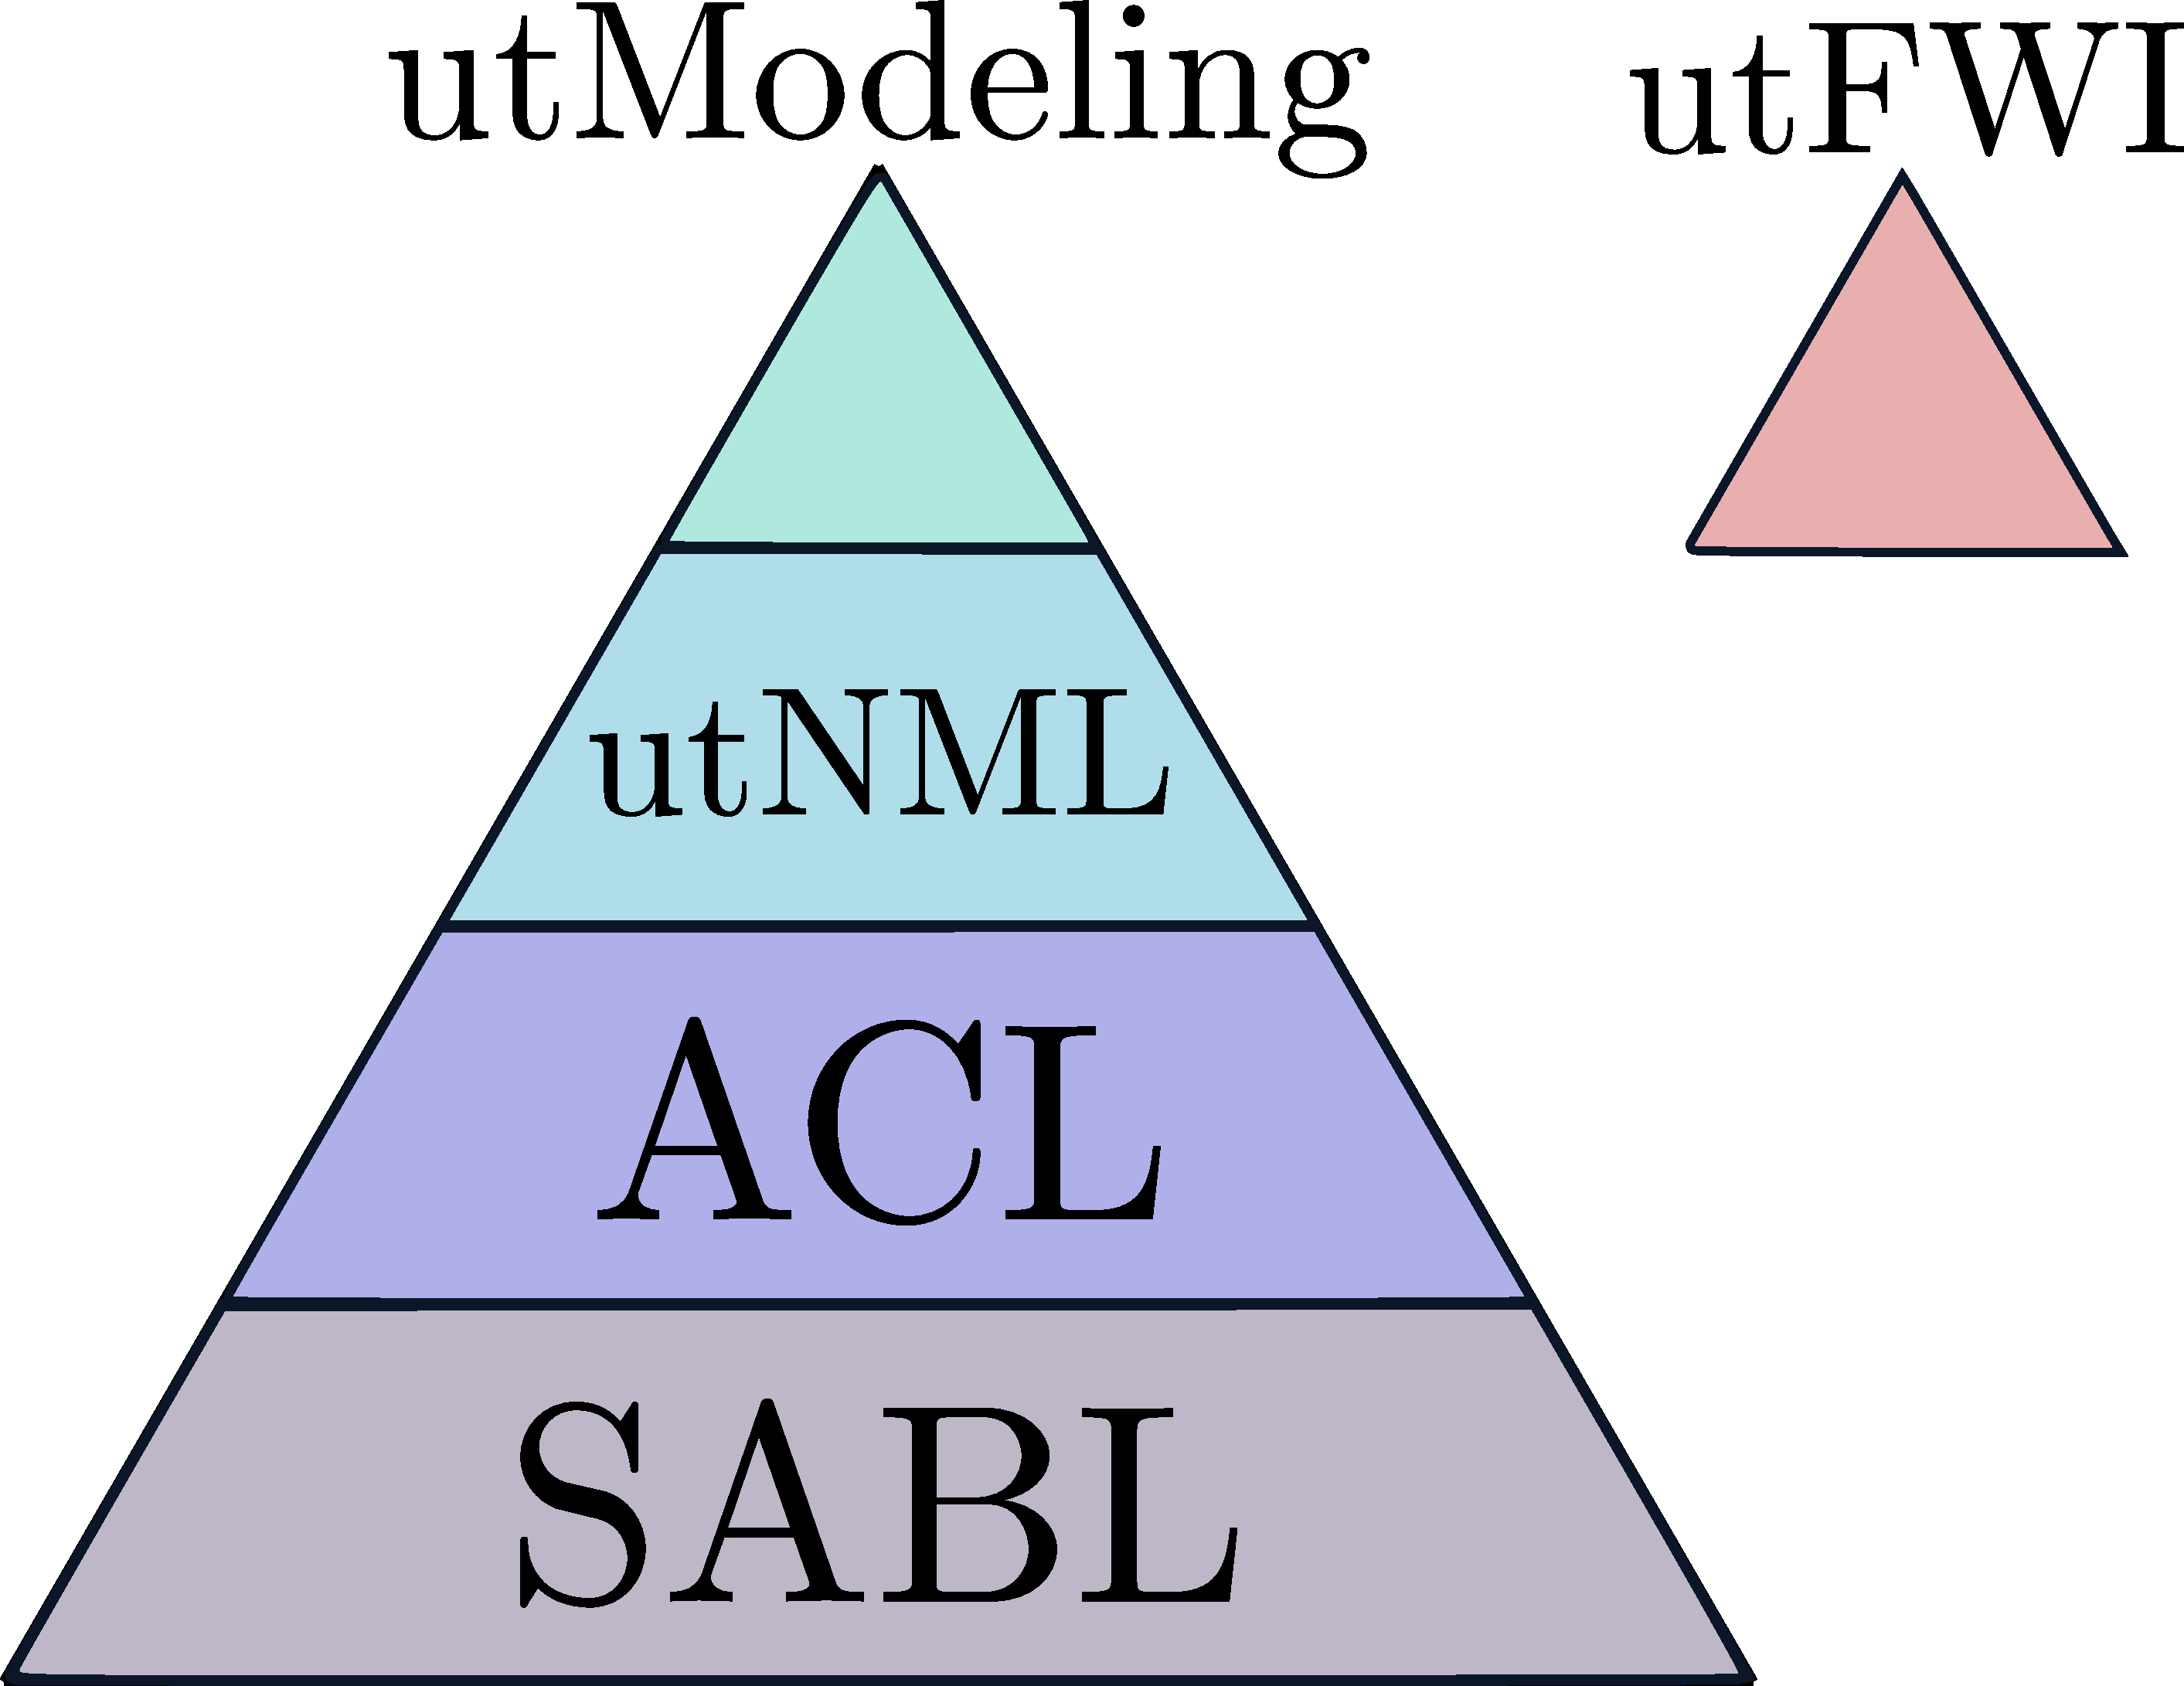
\includegraphics[scale=0.12]{image/carbon.pdf}
%%       \caption*{Illustration of the hierarchical Total's environnement.}
%%       \label{carbon}
%%     \end{figure}

%%     \columnbreak

%%     \begin{itemize}
%%       \small
%%     \item<2-> \textbf{SABL}: Seismic Application Base Library (Seismic acquisition + Parallelism)
%%     \item<3-> \textbf{ACL}: Application Core Library  (Discrete operator + Domain decomposition)
%%     \item<4-> \textbf{utNML}: Unstructured Time-domain Numerical Methods Library (Propagators + Models + Seismic Data management)
%%     \item<5-> \textbf{utModeling}: Unstructured Time-domain Modeling (Main application to perform the modelling)
%%     \end{itemize}
%%   \end{multicols}

%% \end{frame}


\subsection{Parallelism}
\begin{frame}{Parallelism}{Two levels of parallelism}

  \begin{overprint}
    \onslide<2>
  \begin{figure}[H]
    \centering
    
\includegraphics[scale=0.15]{image/partition.png}
    \caption*{$nb\_domain=10$ cores to solve one forward problem (shot) \footnotemark.}
    \label{partition}
  \end{figure}
  \addtocounter{footnote}{-1}
  \footcitetext{karypis1997parmetis}
  \addtocounter{footnote}{+1}
      \onslide<3>
\begin{figure}[H]
  \centering
  \includegraphics[scale=0.055]{image/partition_cluster.pdf}
  \caption*{Illustration of shot parallelism for gradient computation.}
  \label{partition_cluster}
\end{figure}

$nb\_cores = nb\_domain \times nb\_cluster$

  \end{overprint}
\end{frame}



\begin{frame}{Speed-up study for different configurations \newline (120 CPU cores)}{2D experiment on Marmousi (7218 elements - 5 FWI iteration - 20 shots)}

  \begin{figure}
  \pgfplotsset{compat=newest}
    \begin{tikzpicture}
        \begin{axis}[
            grid=major,
            grid style={dashed,gray!30}, %grille de fond
            width=12cm, %largeur histo
            height=6cm, %hauteur histo
            ybar,
            bar width=0.3, %largeur barre
            ymin=1, %à décommenter si tu veux le premier rendu que je t'ai montré
            xticklabel style={rotate=45,font=\footnotesize},
            xticklabels from table={graph/cluster_speed_up.dat}{x}, % use the x column from the file for ticklabels
            xtick=data, % add a tick at every data point,
            enlarge x limits=0.1, % adjust space between axis edge and plot edge
            xlabel={Configuration (nb\_domain, nb\_cluster)},
            ylabel={Elapsed Time (s)},
            nodes near coords, %valeur écrites au-dessus des barres (à enlever si tu n'en veux pas)
            axis line style={ultra thin,gray}, %type et couleur des axes
            axis x line*=bottom,
            axis y line*=left
            ]
            %blur shadow renvoie toujours une erreur, tu peux changer par drop shadow si tu ne veux pas d'erreur
            %blur shadow sort quand même un truc malgré l'erreur
            \addplot[draw=none,fill=col2]table[x expr=\coordindex,y=y] {graph/cluster_speed_up.dat};
        \end{axis}
    \end{tikzpicture}
    \end{figure}



  \end{frame}


% ============================================
% ====== Frame : Marmousi ==================== 4
% ============================================

\begin{frame}{Marmousi}

  \vspace{-0.6cm}
   \begin{multicols}{2}

     \begin{itemize}
       \scriptsize
    \item \textbf{Domain:} 9.2km $\times$ 3km
    \item \textbf{Total time:} 5.2s
    \item \textbf{$\boldsymbol{\nsrc}$/$\boldsymbol{\nrcv}$:} 20 / 183
    \item \textbf{Number of parameters ($\nparam$):} 134142
    \item \textbf{Elapsed time:} 4.6h
    \item \textbf{Parallelism:} 120 CPU ($n\_cluster=20$, $n\_domain=5$)
    \item \textbf{Optimizer:} L-BFGS
    \item \textbf{Noise:} SNR=10
    \end{itemize}

     \columnbreak
     \scriptsize
     \setlength{\modelwidth}{6.0cm}
     \begin{figure}
       \renewcommand{\modelfile}{image/mesh_adapt/wadg_adapt_vp_0}
       \begin{tikzpicture}
  \pgfmathsetmacro{\xmin} {0.}
\pgfmathsetmacro{\xmax} {9.7}
\pgfmathsetmacro{\zmin} {0.}
\pgfmathsetmacro{\zmax} {2.7}
\pgfmathsetmacro{\zzmax} {3.0}
\pgfmathsetmacro{\xxmax} {10.0}

\begin{axis}[%
width=1.0\modelwidth,
height=0.5\modelwidth,
axis on top, separate axis lines,
xmin=\xmin, xmax=\xxmax, %xlabel={x (km)},
ymin=\zmin, ymax=\zzmax,
yticklabels={},xticklabels={},
y dir=reverse,
point meta min=1.5e3, point meta max=5.5e3,
axis x line=top,thick,
axis y line=left,thick,
ylabel style={rotate=-90},
ylabel={$z$},
xlabel={$x$},
ticks = none,
]
\addplot [forget plot] graphics [xmin=\xmin,xmax=\xmax,ymin=\zmin,ymax=\zmax] {{\modelfile}.png};
\end{axis}
\end{tikzpicture}%

       \vspace{-0.3cm}
       \caption*{\scriptsize{Initial wavespeed model.}}
       \label{marmousi_blind_c4}
     \end{figure}
     \vspace{-1.2cm}
     \begin{figure}
       \renewcommand{\modelfile}{image/marmousi}
       \begin{tikzpicture}
  \pgfmathsetmacro{\xmin} {0.}
\pgfmathsetmacro{\xmax} {9.7}
\pgfmathsetmacro{\zmin} {0.}
\pgfmathsetmacro{\zmax} {2.7}
\pgfmathsetmacro{\zzmax} {3.0}
\pgfmathsetmacro{\xxmax} {10.0}

\begin{axis}[%
width=1.0\modelwidth,
height=0.5\modelwidth,
axis on top, separate axis lines,
xmin=\xmin, xmax=\xxmax, %xlabel={x (km)},
ymin=\zmin, ymax=\zzmax,
yticklabels={},xticklabels={},
y dir=reverse,
point meta min=1.5e3, point meta max=5.5e3,
axis x line=top,thick,
axis y line=left,thick,
ylabel style={rotate=-90},
ylabel={$z$},
xlabel={$x$},
ticks = none,
]
\addplot [forget plot] graphics [xmin=\xmin,xmax=\xmax,ymin=\zmin,ymax=\zmax] {{\modelfile}.png};
\end{axis}
\end{tikzpicture}%

       \vspace{-0.3cm}
       \caption*{\scriptsize{Target wavespeed model.}}
       \label{marmousi_blind_c4}
     \end{figure}
     \vspace{-1.2cm}
          \begin{figure}
       \renewcommand{\modelfile}{image/cycle_skipping}
       \begin{tikzpicture}
  \pgfmathsetmacro{\xmin} {0.}
\pgfmathsetmacro{\xmax} {9.7}
\pgfmathsetmacro{\zmin} {0.}
\pgfmathsetmacro{\zmax} {2.7}
\pgfmathsetmacro{\zzmax} {3.0}
\pgfmathsetmacro{\xxmax} {10.0}

\begin{axis}[%
width=1.0\modelwidth,
height=0.5\modelwidth,
axis on top, separate axis lines,
xmin=\xmin, xmax=\xxmax, %xlabel={x (km)},
ymin=\zmin, ymax=\zzmax,
yticklabels={},xticklabels={},
y dir=reverse,
point meta min=1.5e3, point meta max=5.5e3,
axis x line=top,thick,
axis y line=left,thick,
ylabel style={rotate=-90},
ylabel={$z$},
xlabel={$x$},
ticks = none,
]
\addplot [forget plot] graphics [xmin=\xmin,xmax=\xmax,ymin=\zmin,ymax=\zmax] {{\modelfile}.png};
\end{axis}
\end{tikzpicture}%

       \vspace{-0.3cm}
       \caption*{\scriptsize{Cycle-Skipping \footnotemark.}}
       \label{marmousi_blind_c4}
     \end{figure}
   \end{multicols}
   \footcite{bunksMultiscaleSeismicWaveform1995}


\end{frame}



% ============================================
% ====== Frame : Marmousi ==================== 4
% ============================================

\begin{frame}[noframenumbering]{Marmousi}

  \vspace{-0.6cm}
   \begin{multicols}{2}

     \begin{itemize}
       \scriptsize
    \item \textbf{Domain:} 9.2km $\times$ 3km
    \item \textbf{Total time:} 5.2s
    \item \textbf{$\boldsymbol{\nsrc}$/$\boldsymbol{\nrcv}$:} 20 / 183
    \item \textbf{Number of parameters ($\nparam$):} 134142
    \item \textbf{Elapsed time:} 9.8h
    \item \textbf{Parallelism:} 120 CPU ($n\_cluster=20$, $n\_domain=5$)
    \item \textbf{Optimizer:} L-BFGS
    \item \textbf{Noise:} SNR=10 (Signal Nose Ratio)
    \end{itemize}

     \columnbreak
     \scriptsize
     \setlength{\modelwidth}{6.0cm}
     \begin{figure}
       \renewcommand{\modelfile}{image/mesh_adapt/wadg_adapt_vp_0}
       \begin{tikzpicture}
  \pgfmathsetmacro{\xmin} {0.}
\pgfmathsetmacro{\xmax} {9.7}
\pgfmathsetmacro{\zmin} {0.}
\pgfmathsetmacro{\zmax} {2.7}
\pgfmathsetmacro{\zzmax} {3.0}
\pgfmathsetmacro{\xxmax} {10.0}

\begin{axis}[%
width=1.0\modelwidth,
height=0.5\modelwidth,
axis on top, separate axis lines,
xmin=\xmin, xmax=\xxmax, %xlabel={x (km)},
ymin=\zmin, ymax=\zzmax,
yticklabels={},xticklabels={},
y dir=reverse,
point meta min=1.5e3, point meta max=5.5e3,
axis x line=top,thick,
axis y line=left,thick,
ylabel style={rotate=-90},
ylabel={$z$},
xlabel={$x$},
ticks = none,
]
\addplot [forget plot] graphics [xmin=\xmin,xmax=\xmax,ymin=\zmin,ymax=\zmax] {{\modelfile}.png};
\end{axis}
\end{tikzpicture}%

       \vspace{-0.3cm}
       \caption*{\scriptsize{Initial wavespeed model.}}
       \label{marmousi_blind_c4}
     \end{figure}
     \vspace{-1.2cm}
     \begin{figure}
       \renewcommand{\modelfile}{image/marmousi}
       \begin{tikzpicture}
  \pgfmathsetmacro{\xmin} {0.}
\pgfmathsetmacro{\xmax} {9.7}
\pgfmathsetmacro{\zmin} {0.}
\pgfmathsetmacro{\zmax} {2.7}
\pgfmathsetmacro{\zzmax} {3.0}
\pgfmathsetmacro{\xxmax} {10.0}

\begin{axis}[%
width=1.0\modelwidth,
height=0.5\modelwidth,
axis on top, separate axis lines,
xmin=\xmin, xmax=\xxmax, %xlabel={x (km)},
ymin=\zmin, ymax=\zzmax,
yticklabels={},xticklabels={},
y dir=reverse,
point meta min=1.5e3, point meta max=5.5e3,
axis x line=top,thick,
axis y line=left,thick,
ylabel style={rotate=-90},
ylabel={$z$},
xlabel={$x$},
ticks = none,
]
\addplot [forget plot] graphics [xmin=\xmin,xmax=\xmax,ymin=\zmin,ymax=\zmax] {{\modelfile}.png};
\end{axis}
\end{tikzpicture}%

       \vspace{-0.3cm}
       \caption*{\scriptsize{Target wavespeed model.}}
       \label{marmousi_blind_c4}
     \end{figure}
     \vspace{-1.2cm}
          \begin{figure}
       \renewcommand{\modelfile}{image/mesh_adapt/wadg_adapt_vp_100}
       \begin{tikzpicture}
  \pgfmathsetmacro{\xmin} {0.}
\pgfmathsetmacro{\xmax} {9.7}
\pgfmathsetmacro{\zmin} {0.}
\pgfmathsetmacro{\zmax} {2.7}
\pgfmathsetmacro{\zzmax} {3.0}
\pgfmathsetmacro{\xxmax} {10.0}

\begin{axis}[%
width=1.0\modelwidth,
height=0.5\modelwidth,
axis on top, separate axis lines,
xmin=\xmin, xmax=\xxmax, %xlabel={x (km)},
ymin=\zmin, ymax=\zzmax,
yticklabels={},xticklabels={},
y dir=reverse,
point meta min=1.5e3, point meta max=5.5e3,
axis x line=top,thick,
axis y line=left,thick,
ylabel style={rotate=-90},
ylabel={$z$},
xlabel={$x$},
ticks = none,
]
\addplot [forget plot] graphics [xmin=\xmin,xmax=\xmax,ymin=\zmin,ymax=\zmax] {{\modelfile}.png};
\end{axis}
\end{tikzpicture}%

       \vspace{-0.3cm}
       \caption*{\scriptsize{Reconstructed wavespeed model.}}
       \label{marmousi_blind_c4}
     \end{figure}
   \end{multicols}

   \vspace{-1cm}
   \begin{table}[H]
     \scriptsize
     \centering
     \begin{tabular}{|c|c|c|c|c|c|c|}
       \hline
       Filter          & {[}0,2Hz{]} & {[}0,5Hz{]} & {[}0,8Hz{]} & {[}0,12Hz{]}& {[}0,15Hz{]}  & Total \\ \hline
       Nb of iterations& 20          & 20          & 20          & 20          &    20         & 100   \\ \hline
     \end{tabular}
     \label{freq_overthrust}
   \end{table}


\end{frame}


% ============================================
% ====== Frame : Overthrust ================== 4
% ============================================

\begin{frame}{Overthrust 2D}

  \vspace{-0.6cm}
   \begin{multicols}{2}

     \begin{itemize}
       \scriptsize
    \item \textbf{Domain:} 20km $\times$ 4.65km
    \item \textbf{Total time:} 5.2s
    \item \textbf{$\boldsymbol{\nsrc}$/$\boldsymbol{\nrcv}$:} 30 / 391
    \item \textbf{Number of parameters ($\nparam$):} 20678
    \item \textbf{Elapsed time:} 20.5h
    \item \textbf{Parallelism:} 120 CPU ($n\_cluster=10$, $n\_domain=12$)
    \item \textbf{Optimizer:} L-BFGS
     \end{itemize}

     \columnbreak
     \scriptsize
     \setlength{\modelwidth}{6.0cm}
     \begin{figure}
       \renewcommand{\modelfile}{image/mesh_adapt/overthrust_ini_paraview}
       \begin{tikzpicture}
  \pgfmathsetmacro{\xmin} {0.}
\pgfmathsetmacro{\xmax} {9.7}
\pgfmathsetmacro{\zmin} {0.}
\pgfmathsetmacro{\zmax} {2.7}
\pgfmathsetmacro{\zzmax} {3.0}
\pgfmathsetmacro{\xxmax} {10.0}

\begin{axis}[%
width=1.0\modelwidth,
height=0.5\modelwidth,
axis on top, separate axis lines,
xmin=\xmin, xmax=\xxmax, %xlabel={x (km)},
ymin=\zmin, ymax=\zzmax,
yticklabels={},xticklabels={},
y dir=reverse,
point meta min=1.5e3, point meta max=5.5e3,
axis x line=top,thick,
axis y line=left,thick,
ylabel style={rotate=-90},
ylabel={$z$},
xlabel={$x$},
ticks = none,
]
\addplot [forget plot] graphics [xmin=\xmin,xmax=\xmax,ymin=\zmin,ymax=\zmax] {{\modelfile}.png};
\end{axis}
\end{tikzpicture}%

       \vspace{-0.3cm}
       \caption*{\scriptsize{Initial wavespeed model.}}
       \label{marmousi_blind_c4}
     \end{figure}
     \vspace{-1.2cm}
     \begin{figure}
       \renewcommand{\modelfile}{image/mesh_adapt/overthrust}
       \begin{tikzpicture}
  \pgfmathsetmacro{\xmin} {0.}
\pgfmathsetmacro{\xmax} {9.7}
\pgfmathsetmacro{\zmin} {0.}
\pgfmathsetmacro{\zmax} {2.7}
\pgfmathsetmacro{\zzmax} {3.0}
\pgfmathsetmacro{\xxmax} {10.0}

\begin{axis}[%
width=1.0\modelwidth,
height=0.5\modelwidth,
axis on top, separate axis lines,
xmin=\xmin, xmax=\xxmax, %xlabel={x (km)},
ymin=\zmin, ymax=\zzmax,
yticklabels={},xticklabels={},
y dir=reverse,
point meta min=1.5e3, point meta max=5.5e3,
axis x line=top,thick,
axis y line=left,thick,
ylabel style={rotate=-90},
ylabel={$z$},
xlabel={$x$},
ticks = none,
]
\addplot [forget plot] graphics [xmin=\xmin,xmax=\xmax,ymin=\zmin,ymax=\zmax] {{\modelfile}.png};
\end{axis}
\end{tikzpicture}%

       \vspace{-0.3cm}
       \caption*{\scriptsize{Target wavespeed model.}}
       \label{marmousi_blind_c4}
     \end{figure}
     \vspace{-1.2cm}
          \begin{figure}
       \renewcommand{\modelfile}{image/overthrust_final_p2}
       \begin{tikzpicture}
  \pgfmathsetmacro{\xmin} {0.}
\pgfmathsetmacro{\xmax} {9.7}
\pgfmathsetmacro{\zmin} {0.}
\pgfmathsetmacro{\zmax} {2.7}
\pgfmathsetmacro{\zzmax} {3.0}
\pgfmathsetmacro{\xxmax} {10.0}

\begin{axis}[%
width=1.0\modelwidth,
height=0.5\modelwidth,
axis on top, separate axis lines,
xmin=\xmin, xmax=\xxmax, %xlabel={x (km)},
ymin=\zmin, ymax=\zzmax,
yticklabels={},xticklabels={},
y dir=reverse,
point meta min=1.5e3, point meta max=5.5e3,
axis x line=top,thick,
axis y line=left,thick,
ylabel style={rotate=-90},
ylabel={$z$},
xlabel={$x$},
ticks = none,
]
\addplot [forget plot] graphics [xmin=\xmin,xmax=\xmax,ymin=\zmin,ymax=\zmax] {{\modelfile}.png};
\end{axis}
\end{tikzpicture}%

       \vspace{-0.3cm}
       \caption*{\scriptsize{Reconstructed wavespeed model.}}
       \label{marmousi_blind_c4}
     \end{figure}


   \end{multicols}

   \vspace{-1cm}
   \begin{table}[H]
     \scriptsize
  \centering
\begin{tabular}{|c|c|c|c|c|c|c|}
\hline
Filter          & {[}0,2Hz{]} & {[}0,5Hz{]} & {[}0,8Hz{]} & {[}0,12Hz{]}& {[}0,15Hz{]}  & Total \\ \hline
Nb of iterations& 20          & 20          & 20          & 20          &    20         & 100   \\ \hline
\end{tabular}
\label{freq_overthrust}
\end{table}

\end{frame}



% ============================================
% ====== Frame : Sigsbee ================== 4
% ============================================

\begin{frame}{Sigsbee}

  \vspace{-0.6cm}
   \begin{multicols}{2}

     \begin{itemize}
       \scriptsize
    \item \textbf{Domain:} 20.4km $\times$ 9.1km
    \item \textbf{Total time:} 7.2s
    \item \textbf{$\boldsymbol{\nsrc}$/$\boldsymbol{\nrcv}$:} 72 / 320
    \item \textbf{Number of parameters ($\nparam$):} 20454
    \item \textbf{Elapsed time:} 23.3h
    \item \textbf{Parallelism:} 120 CPU ($n\_cluster=12$, $n\_domain=10$)
    \item \textbf{Optimizer:} L-BFGS
     \end{itemize}

     \columnbreak
     \scriptsize
     \setlength{\modelwidth}{6.0cm}
     \begin{figure}
       \renewcommand{\modelfile}{image/sigsbee_ini}
       \begin{tikzpicture}
  \pgfmathsetmacro{\xmin} {0.}
\pgfmathsetmacro{\xmax} {9.7}
\pgfmathsetmacro{\zmin} {0.}
\pgfmathsetmacro{\zmax} {2.7}
\pgfmathsetmacro{\zzmax} {3.0}
\pgfmathsetmacro{\xxmax} {10.0}

\begin{axis}[%
width=1.0\modelwidth,
height=0.5\modelwidth,
axis on top, separate axis lines,
xmin=\xmin, xmax=\xxmax, %xlabel={x (km)},
ymin=\zmin, ymax=\zzmax,
yticklabels={},xticklabels={},
y dir=reverse,
point meta min=1.5e3, point meta max=5.5e3,
axis x line=top,thick,
axis y line=left,thick,
ylabel style={rotate=-90},
ylabel={$z$},
xlabel={$x$},
ticks = none,
]
\addplot [forget plot] graphics [xmin=\xmin,xmax=\xmax,ymin=\zmin,ymax=\zmax] {{\modelfile}.png};
\end{axis}
\end{tikzpicture}%

       \vspace{-0.3cm}
       \caption*{\scriptsize{Initial wavespeed model.}}
       \label{marmousi_blind_c4}
     \end{figure}
     \vspace{-1.2cm}
     \begin{figure}
       \renewcommand{\modelfile}{image/sigsbee}
       \begin{tikzpicture}
  \pgfmathsetmacro{\xmin} {0.}
\pgfmathsetmacro{\xmax} {9.7}
\pgfmathsetmacro{\zmin} {0.}
\pgfmathsetmacro{\zmax} {2.7}
\pgfmathsetmacro{\zzmax} {3.0}
\pgfmathsetmacro{\xxmax} {10.0}

\begin{axis}[%
width=1.0\modelwidth,
height=0.5\modelwidth,
axis on top, separate axis lines,
xmin=\xmin, xmax=\xxmax, %xlabel={x (km)},
ymin=\zmin, ymax=\zzmax,
yticklabels={},xticklabels={},
y dir=reverse,
point meta min=1.5e3, point meta max=5.5e3,
axis x line=top,thick,
axis y line=left,thick,
ylabel style={rotate=-90},
ylabel={$z$},
xlabel={$x$},
ticks = none,
]
\addplot [forget plot] graphics [xmin=\xmin,xmax=\xmax,ymin=\zmin,ymax=\zmax] {{\modelfile}.png};
\end{axis}
\end{tikzpicture}%

       \vspace{-0.3cm}
       \caption*{\scriptsize{Target wavespeed model.}}
       \label{marmousi_blind_c4}
     \end{figure}
     \vspace{-1.2cm}
          \begin{figure}
       \renewcommand{\modelfile}{image/sigsbee_final}
       \begin{tikzpicture}
  \pgfmathsetmacro{\xmin} {0.}
\pgfmathsetmacro{\xmax} {9.7}
\pgfmathsetmacro{\zmin} {0.}
\pgfmathsetmacro{\zmax} {2.7}
\pgfmathsetmacro{\zzmax} {3.0}
\pgfmathsetmacro{\xxmax} {10.0}

\begin{axis}[%
width=1.0\modelwidth,
height=0.5\modelwidth,
axis on top, separate axis lines,
xmin=\xmin, xmax=\xxmax, %xlabel={x (km)},
ymin=\zmin, ymax=\zzmax,
yticklabels={},xticklabels={},
y dir=reverse,
point meta min=1.5e3, point meta max=5.5e3,
axis x line=top,thick,
axis y line=left,thick,
ylabel style={rotate=-90},
ylabel={$z$},
xlabel={$x$},
ticks = none,
]
\addplot [forget plot] graphics [xmin=\xmin,xmax=\xmax,ymin=\zmin,ymax=\zmax] {{\modelfile}.png};
\end{axis}
\end{tikzpicture}%

       \vspace{-0.3cm}
       \caption*{\scriptsize{Reconstructed wavespeed model.}}
       \label{marmousi_blind_c4}
     \end{figure}

   \end{multicols}

   \vspace{-1cm}
   \scriptsize
\begin{table}[H]
  \centering
\begin{tabular}{|c|c|c|c|c|c|c|}
\hline
Filter           & {[}0,2Hz{]} & {[}0,5Hz{]} & {[}0,7Hz{]} & {[}0,10Hz{]}  & Total \\ \hline
Nb of iterations & 30          & 20          & 15            & 10          & 75    \\ \hline
\end{tabular}
\end{table}
\end{frame}




% ============================================
% ====== Frame : Sigsbee ================== 4
% ============================================

\begin{frame}[noframenumbering]{Sigsbee}

  \vspace{-0.6cm}
   \begin{multicols}{2}

     \begin{itemize}
       \scriptsize
    \item \textbf{Domain:} 20.4km $\times$ 9.1km
    \item \textbf{Total time:} 7.2s
    \item \textbf{$\boldsymbol{\nsrc}$/$\boldsymbol{\nrcv}$:} 72 / 320
    \item \textbf{Number of parameters ($\nparam$):} 20454
    \item \textbf{Elapsed time:} $\approx$20h
    \item \textbf{Parallelism:} 120 CPU ($n\_cluster=12$, $n\_domain=10$)
    \item \textbf{Optimizer:} L-BFGS
     \end{itemize}

     \columnbreak
     \scriptsize
     \setlength{\modelwidth}{6.0cm}
     \begin{figure}
       \renewcommand{\modelfile}{image/sigsbee_ini}
       \begin{tikzpicture}
  \pgfmathsetmacro{\xmin} {0.}
\pgfmathsetmacro{\xmax} {9.7}
\pgfmathsetmacro{\zmin} {0.}
\pgfmathsetmacro{\zmax} {2.7}
\pgfmathsetmacro{\zzmax} {3.0}
\pgfmathsetmacro{\xxmax} {10.0}

\begin{axis}[%
width=1.0\modelwidth,
height=0.5\modelwidth,
axis on top, separate axis lines,
xmin=\xmin, xmax=\xxmax, %xlabel={x (km)},
ymin=\zmin, ymax=\zzmax,
yticklabels={},xticklabels={},
y dir=reverse,
point meta min=1.5e3, point meta max=5.5e3,
axis x line=top,thick,
axis y line=left,thick,
ylabel style={rotate=-90},
ylabel={$z$},
xlabel={$x$},
ticks = none,
]
\addplot [forget plot] graphics [xmin=\xmin,xmax=\xmax,ymin=\zmin,ymax=\zmax] {{\modelfile}.png};
\end{axis}
\end{tikzpicture}%

       \vspace{-0.3cm}
       \caption*{\scriptsize{Initial wavespeed model.}}
       \label{marmousi_blind_c4}
     \end{figure}
     \vspace{-1.2cm}
     \begin{figure}
       \renewcommand{\modelfile}{image/sigsbee}
       \begin{tikzpicture}
  \pgfmathsetmacro{\xmin} {0.}
\pgfmathsetmacro{\xmax} {9.7}
\pgfmathsetmacro{\zmin} {0.}
\pgfmathsetmacro{\zmax} {2.7}
\pgfmathsetmacro{\zzmax} {3.0}
\pgfmathsetmacro{\xxmax} {10.0}

\begin{axis}[%
width=1.0\modelwidth,
height=0.5\modelwidth,
axis on top, separate axis lines,
xmin=\xmin, xmax=\xxmax, %xlabel={x (km)},
ymin=\zmin, ymax=\zzmax,
yticklabels={},xticklabels={},
y dir=reverse,
point meta min=1.5e3, point meta max=5.5e3,
axis x line=top,thick,
axis y line=left,thick,
ylabel style={rotate=-90},
ylabel={$z$},
xlabel={$x$},
ticks = none,
]
\addplot [forget plot] graphics [xmin=\xmin,xmax=\xmax,ymin=\zmin,ymax=\zmax] {{\modelfile}.png};
\end{axis}
\end{tikzpicture}%

       \vspace{-0.3cm}
       \caption*{\scriptsize{Target wavespeed model.}}
       \label{marmousi_blind_c4}
     \end{figure}
     \vspace{-1.2cm}
          \begin{figure}
       \renewcommand{\modelfile}{image/sigsbee_low_freq}
       \begin{tikzpicture}
  \pgfmathsetmacro{\xmin} {0.}
\pgfmathsetmacro{\xmax} {9.7}
\pgfmathsetmacro{\zmin} {0.}
\pgfmathsetmacro{\zmax} {2.7}
\pgfmathsetmacro{\zzmax} {3.0}
\pgfmathsetmacro{\xxmax} {10.0}

\begin{axis}[%
width=1.0\modelwidth,
height=0.5\modelwidth,
axis on top, separate axis lines,
xmin=\xmin, xmax=\xxmax, %xlabel={x (km)},
ymin=\zmin, ymax=\zzmax,
yticklabels={},xticklabels={},
y dir=reverse,
point meta min=1.5e3, point meta max=5.5e3,
axis x line=top,thick,
axis y line=left,thick,
ylabel style={rotate=-90},
ylabel={$z$},
xlabel={$x$},
ticks = none,
]
\addplot [forget plot] graphics [xmin=\xmin,xmax=\xmax,ymin=\zmin,ymax=\zmax] {{\modelfile}.png};
\end{axis}
\end{tikzpicture}%

       \vspace{-0.3cm}
       \caption*{\scriptsize{Reconstructed wavespeed model.}}
       \label{marmousi_blind_c4}
     \end{figure}

   \end{multicols}

   \vspace{-1cm}
   \scriptsize
\begin{table}[H]
  \centering
\begin{tabular}{|c|c|c|c|c|c|c|c|}
\hline
Filter           & {[}0,0.5Hz{]} & {[}0,1Hz{]} & {[}0,1.5Hz{]} & {[}0,2Hz{]} & {[}0,4Hz{]} & {[}0,6Hz{]}   & Total \\ \hline
Nb of iterations & 20          & 20          & 20              & 20          & 20          & 20            &  120    \\ \hline
\end{tabular}
\end{table}
\end{frame}








% ============================================
% ====== Frame : SEAM ================== 4
% ============================================

\begin{frame}{SEAM Foothills (Reduced) 3D}

  \vspace{-0.6cm}
   \begin{multicols}{2}

     \begin{itemize}
       \scriptsize
    \item \textbf{Domain}: (3km $\times$ 3km $\times$ 3.5km) subcube;
    \item \textbf{Total time:} 3.2s
    \item \textbf{$\boldsymbol{\nsrc}$/$\boldsymbol{\nrcv}$:} 30 / 1225
    \item \textbf{TRANSMISSION CONFIGURATION}
      \columnbreak
    \item \textbf{Number of parameters ($\nparam$):} 943008
    \item \textbf{Elapsed time:} 4.2 days
    \item \textbf{Parallelism:} 360 CPU ($n\_cluster=30$, $n\_domain=12$)
    \item \textbf{Optimizer:} L-BFGS
     \end{itemize}
   \end{multicols}
     \scriptsize
     \setlength{\modelwidth}{4.5cm}

\begin{figure}[!htbp]
\begin{subfigure}{0.3\textwidth}
\renewcommand{\modelfile}{image/seam0_y1}
\begin{tikzpicture}
\pgfmathsetmacro{\xmin} {0.}
\pgfmathsetmacro{\zmin} {0.}
\pgfmathsetmacro{\xmax} {9.5}
\pgfmathsetmacro{\zmax} {9.5}
\pgfmathsetmacro{\xxmax} {10.0}
\pgfmathsetmacro{\zzmax} {10.0}


\begin{axis}[%
width=1.0\modelwidth,
height=1.0\modelwidth,
axis on top, separate axis lines,
xmin=\xmin, xmax=\xxmax, %xlabel={x (km)},
ymin=\zmin, ymax=\zzmax,
yticklabels={},xticklabels={},
y dir=reverse,
point meta min=1.5e3, point meta max=5.5e3,
axis x line=top,thick,
axis y line=left,thick,
ylabel style={rotate=-90},
ylabel={$z$},
xlabel={$x$},
ticks = none,
]
\addplot [forget plot] graphics [xmin=\xmin,xmax=\xmax,ymin=\zmin,ymax=\zmax] {{\modelfile}.png};
\end{axis}
\end{tikzpicture}%

\caption*{\scriptsize{Initial wavespeed model  at $y=6530$m.}}
\end{subfigure}
\begin{subfigure}{0.3\textwidth}
\renewcommand{\modelfile}{image/seam1_y1}
\begin{tikzpicture}
\pgfmathsetmacro{\xmin} {0.}
\pgfmathsetmacro{\zmin} {0.}
\pgfmathsetmacro{\xmax} {9.5}
\pgfmathsetmacro{\zmax} {9.5}
\pgfmathsetmacro{\xxmax} {10.0}
\pgfmathsetmacro{\zzmax} {10.0}


\begin{axis}[%
width=1.0\modelwidth,
height=1.0\modelwidth,
axis on top, separate axis lines,
xmin=\xmin, xmax=\xxmax, %xlabel={x (km)},
ymin=\zmin, ymax=\zzmax,
yticklabels={},xticklabels={},
y dir=reverse,
point meta min=1.5e3, point meta max=5.5e3,
axis x line=top,thick,
axis y line=left,thick,
ylabel style={rotate=-90},
ylabel={$z$},
xlabel={$x$},
ticks = none,
]
\addplot [forget plot] graphics [xmin=\xmin,xmax=\xmax,ymin=\zmin,ymax=\zmax] {{\modelfile}.png};
\end{axis}
\end{tikzpicture}%

\caption*{\scriptsize{Reconstructed wavespeed model at $y=6530$m.}}
\end{subfigure}
\begin{subfigure}{0.3\textwidth}
  \vspace{-0.4cm}
\renewcommand{\modelfile}{image/seam2_y1}
\renewcommand{\cmapmin}{2000}
\renewcommand{\cmapmax}{6000}
\begin{tikzpicture}
\pgfmathsetmacro{\xmin} {0.}
\pgfmathsetmacro{\zmin} {0.}
\pgfmathsetmacro{\xmax} {9.5}
\pgfmathsetmacro{\zmax} {9.5}
\pgfmathsetmacro{\xxmax} {10.}
\pgfmathsetmacro{\zzmax} {10.}



\begin{axis}[%
width=1.0\modelwidth,
height=1.0\modelwidth,
axis on top, separate axis lines,
xmin=\xmin, xmax=\xxmax, %xlabel={x (km)},
ymin=\zmin, ymax=\zzmax,
yticklabels={},xticklabels={},
y dir=reverse,
colormap/paraview, colorbar,
colorbar style={title=\small{$m \cdot s^{-1}$}},
point meta min=\cmapmin, point meta max=\cmapmax,
colorbar/width=2.5mm,
axis x line=top,thick,
axis y line=left,thick,
ylabel style={rotate=-90},
ylabel={$z$},
xlabel={$x$},
ticks = none,
]
\addplot [forget plot] graphics [xmin=\xmin,xmax=\xmax,ymin=\zmin,ymax=\zmax] {{\modelfile}.png};
\end{axis}
\end{tikzpicture}%

\vspace{-0.8cm}
\caption*{\scriptsize{Target wavespeed model at $y=6530$m.}}
\end{subfigure}
\end{figure}
\end{frame}


\begin{frame}{SEAM Foothills (Reduced) 3D}

  \vspace{-0.6cm}
   \begin{multicols}{2}

     \begin{itemize}
       \scriptsize
    \item \textbf{Domain}: (3km $\times$ 3km $\times$ 3.5km) subcube;
    \item \textbf{Total time:} 3.2s
    \item \textbf{$\boldsymbol{\nsrc}$/$\boldsymbol{\nrcv}$:} 30 / 1225
    \item \textbf{TRANSMISSION CONFIGURATION}
      \columnbreak
    \item \textbf{Number of parameters ($\nparam$):} 943008
    \item \textbf{Elapsed time:} 4.2 days
    \item \textbf{Parallelism:} 360 CPU ($n\_cluster=30$, $n\_domain=12$)
    \item \textbf{Optimizer:} L-BFGS
     \end{itemize}
   \end{multicols}
     \scriptsize
     \setlength{\modelwidth}{4.5cm}

\begin{figure}[!htbp]
\begin{subfigure}{0.3\textwidth}
\renewcommand{\modelfile}{image/seam1_y1}
\begin{tikzpicture}
\pgfmathsetmacro{\xmin} {0.}
\pgfmathsetmacro{\zmin} {0.}
\pgfmathsetmacro{\xmax} {9.5}
\pgfmathsetmacro{\zmax} {9.5}
\pgfmathsetmacro{\xxmax} {10.0}
\pgfmathsetmacro{\zzmax} {10.0}


\begin{axis}[%
width=1.0\modelwidth,
height=1.0\modelwidth,
axis on top, separate axis lines,
xmin=\xmin, xmax=\xxmax, %xlabel={x (km)},
ymin=\zmin, ymax=\zzmax,
yticklabels={},xticklabels={},
y dir=reverse,
point meta min=1.5e3, point meta max=5.5e3,
axis x line=top,thick,
axis y line=left,thick,
ylabel style={rotate=-90},
ylabel={$z$},
xlabel={$x$},
ticks = none,
]
\addplot [forget plot] graphics [xmin=\xmin,xmax=\xmax,ymin=\zmin,ymax=\zmax] {{\modelfile}.png};
\end{axis}
\end{tikzpicture}%

\caption*{\scriptsize{Reconstructed wavespeed model at $y=6530$m.}}
\end{subfigure}
\setlength{\plotwidth}{4cm}
\setlength{\plotheight}{3.0cm}
\begin{subfigure}{0.3\textwidth}
\centering
    \begin{tikzpicture}
      \begin{axis}[%
          width=\plotwidth, height=\plotheight,,
          at={(0,0)},scale only axis,separate axis lines,
          xlabel={iterations},
          ylabel={$\CF/max(\CF)$},
%          ymode=log,
          %xmin=0,xmax=1,
%          ymin=0,ymax=1,
          legend pos=outer north east
          %ymin=0.98,ymax=1.22
        ]


        \addplot[color=blue,mark options={solid}, mark=triangle*,
        line width=0.8pt,
        mark size=0pt]
        table[x=x,y=y]
        {graph/run_seam.txt};
%        \addlegendentry{L-BFGS}


\end{axis}
\end{tikzpicture}
\label{cf_seam}
\end{subfigure}

\end{figure}
\end{frame}


\begin{frame}[noframenumbering]{SEAM Foothills (Reduced) 3D}

  \vspace{-0.6cm}
   \begin{multicols}{2}

     \begin{itemize}
       \scriptsize
    \item \textbf{Domain}: (3km $\times$ 3km $\times$ 3.5km) subcube;
    \item \textbf{Total time:} 3.2s
    \item \textbf{$\boldsymbol{\nsrc}$/$\boldsymbol{\nrcv}$:} 30 / 1225
    \item \textbf{TRANSMISSION CONFIGURATION}
      \columnbreak
    \item \textbf{Number of parameters ($\nparam$):} 943008
    \item \textbf{Elapsed time:} 4.2 days
    \item \textbf{Parallelism:} 360 CPU ($n\_cluster=30$, $n\_domain=12$)
    \item \textbf{Optimizer:} L-BFGS
     \end{itemize}
   \end{multicols}
     \scriptsize
     \setlength{\modelwidth}{4.5cm}

\begin{figure}[!htbp]
\begin{subfigure}{0.3\textwidth}
\renewcommand{\modelfile}{image/seam0_x1}
\begin{tikzpicture}
\pgfmathsetmacro{\xmin} {0.}
\pgfmathsetmacro{\zmin} {0.}
\pgfmathsetmacro{\xmax} {9.5}
\pgfmathsetmacro{\zmax} {9.5}
\pgfmathsetmacro{\xxmax} {10.0}
\pgfmathsetmacro{\zzmax} {10.0}


\begin{axis}[%
width=1.0\modelwidth,
height=1.0\modelwidth,
axis on top, separate axis lines,
xmin=\xmin, xmax=\xxmax, %xlabel={x (km)},
ymin=\zmin, ymax=\zzmax,
yticklabels={},xticklabels={},
y dir=reverse,
point meta min=1.5e3, point meta max=5.5e3,
axis x line=top,thick,
axis y line=left,thick,
ylabel style={rotate=-90},
ylabel={$z$},
xlabel={$y$},
ticks = none,
]
\addplot [forget plot] graphics [xmin=\xmin,xmax=\xmax,ymin=\zmin,ymax=\zmax] {{\modelfile}.png};
\end{axis}
\end{tikzpicture}%

\caption*{\scriptsize{Initial wavespeed model  at $x=6530$m.}}
\end{subfigure}
\begin{subfigure}{0.3\textwidth}
\renewcommand{\modelfile}{image/seam1_x1}
\begin{tikzpicture}
\pgfmathsetmacro{\xmin} {0.}
\pgfmathsetmacro{\zmin} {0.}
\pgfmathsetmacro{\xmax} {9.5}
\pgfmathsetmacro{\zmax} {9.5}
\pgfmathsetmacro{\xxmax} {10.0}
\pgfmathsetmacro{\zzmax} {10.0}


\begin{axis}[%
width=1.0\modelwidth,
height=1.0\modelwidth,
axis on top, separate axis lines,
xmin=\xmin, xmax=\xxmax, %xlabel={x (km)},
ymin=\zmin, ymax=\zzmax,
yticklabels={},xticklabels={},
y dir=reverse,
point meta min=1.5e3, point meta max=5.5e3,
axis x line=top,thick,
axis y line=left,thick,
ylabel style={rotate=-90},
ylabel={$z$},
xlabel={$y$},
ticks = none,
]
\addplot [forget plot] graphics [xmin=\xmin,xmax=\xmax,ymin=\zmin,ymax=\zmax] {{\modelfile}.png};
\end{axis}
\end{tikzpicture}%

\caption*{\scriptsize{Reconstructed wavespeed model at $x=6530$m.}}
\end{subfigure}
\begin{subfigure}{0.3\textwidth}
  \vspace{-0.4cm}
\renewcommand{\modelfile}{image/seam2_x1}
\renewcommand{\cmapmin}{2000}
\renewcommand{\cmapmax}{6000}
\begin{tikzpicture}
\pgfmathsetmacro{\xmin} {0.}
\pgfmathsetmacro{\zmin} {0.}
\pgfmathsetmacro{\xmax} {9.5}
\pgfmathsetmacro{\zmax} {9.5}
\pgfmathsetmacro{\xxmax} {10.}
\pgfmathsetmacro{\zzmax} {10.}



\begin{axis}[%
width=1.0\modelwidth,
height=1.0\modelwidth,
axis on top, separate axis lines,
xmin=\xmin, xmax=\xxmax, %xlabel={x (km)},
ymin=\zmin, ymax=\zzmax,
yticklabels={},xticklabels={},
y dir=reverse,
colormap/paraview, colorbar,
colorbar style={title=\small{$m \cdot s^{-1}$}},
point meta min=\cmapmin, point meta max=\cmapmax,
colorbar/width=2.5mm,
axis x line=top,thick,
axis y line=left,thick,
ylabel style={rotate=-90},
ylabel={$z$},
xlabel={$y$},
ticks = none,
]
\addplot [forget plot] graphics [xmin=\xmin,xmax=\xmax,ymin=\zmin,ymax=\zmax] {{\modelfile}.png};
\end{axis}
\end{tikzpicture}%

\vspace{-0.8cm}
\caption*{\scriptsize{Target wavespeed model at $x=6530$m.}}
\end{subfigure}
\end{figure}
\end{frame}



\begin{frame}[noframenumbering]{SEAM Foothills (Reduced) 3D}

  \vspace{-0.6cm}
   \begin{multicols}{2}

     \begin{itemize}
       \scriptsize
    \item \textbf{Domain}: (3km $\times$ 3km $\times$ 3.5km) subcube;
    \item \textbf{Total time:} 3.2s
    \item \textbf{$\boldsymbol{\nsrc}$/$\boldsymbol{\nrcv}$:} 30 / 1225
    \item \textbf{TRANSMISSION CONFIGURATION}
      \columnbreak
    \item \textbf{Number of parameters ($\nparam$):} 943008
    \item \textbf{Elapsed time:} 4.2 days
    \item \textbf{Parallelism:} 360 CPU ($n\_cluster=30$, $n\_domain=12$)
    \item \textbf{Optimizer:} L-BFGS
     \end{itemize}
   \end{multicols}
     \scriptsize
     \setlength{\modelwidth}{4.5cm}

\begin{figure}[!htbp]
\begin{subfigure}{0.3\textwidth}
\renewcommand{\modelfile}{image/seam0_z1}
\begin{tikzpicture}
\pgfmathsetmacro{\xmin} {0.}
\pgfmathsetmacro{\zmin} {0.}
\pgfmathsetmacro{\xmax} {9.5}
\pgfmathsetmacro{\zmax} {9.5}
\pgfmathsetmacro{\xxmax} {10.0}
\pgfmathsetmacro{\zzmax} {10.0}


\begin{axis}[%
width=1.0\modelwidth,
height=1.0\modelwidth,
axis on top, separate axis lines,
xmin=\xmin, xmax=\xxmax, %xlabel={x (km)},
ymin=\zmin, ymax=\zzmax,
yticklabels={},xticklabels={},
y dir=reverse,
point meta min=1.5e3, point meta max=5.5e3,
axis x line=top,thick,
axis y line=left,thick,
ylabel style={rotate=-90},
ylabel={$x$},
xlabel={$y$},
ticks = none,
]
\addplot [forget plot] graphics [xmin=\xmin,xmax=\xmax,ymin=\zmin,ymax=\zmax] {{\modelfile}.png};
\end{axis}
\end{tikzpicture}%

\caption*{\scriptsize{Initial wavespeed model  at $z=4950$m.}}
\end{subfigure}
\begin{subfigure}{0.3\textwidth}
\renewcommand{\modelfile}{image/seam1_z1}
\begin{tikzpicture}
\pgfmathsetmacro{\xmin} {0.}
\pgfmathsetmacro{\zmin} {0.}
\pgfmathsetmacro{\xmax} {9.5}
\pgfmathsetmacro{\zmax} {9.5}
\pgfmathsetmacro{\xxmax} {10.0}
\pgfmathsetmacro{\zzmax} {10.0}


\begin{axis}[%
width=1.0\modelwidth,
height=1.0\modelwidth,
axis on top, separate axis lines,
xmin=\xmin, xmax=\xxmax, %xlabel={x (km)},
ymin=\zmin, ymax=\zzmax,
yticklabels={},xticklabels={},
y dir=reverse,
point meta min=1.5e3, point meta max=5.5e3,
axis x line=top,thick,
axis y line=left,thick,
ylabel style={rotate=-90},
ylabel={$x$},
xlabel={$y$},
ticks = none,
]
\addplot [forget plot] graphics [xmin=\xmin,xmax=\xmax,ymin=\zmin,ymax=\zmax] {{\modelfile}.png};
\end{axis}
\end{tikzpicture}%

\caption*{\scriptsize{Reconstructed wavespeed model at $z=4950$m.}}
\end{subfigure}
\begin{subfigure}{0.3\textwidth}
  \vspace{-0.4cm}
\renewcommand{\modelfile}{image/seam2_z1}
\renewcommand{\cmapmin}{2000}
\renewcommand{\cmapmax}{6000}
\begin{tikzpicture}
\pgfmathsetmacro{\xmin} {0.}
\pgfmathsetmacro{\zmin} {0.}
\pgfmathsetmacro{\xmax} {9.5}
\pgfmathsetmacro{\zmax} {9.5}
\pgfmathsetmacro{\xxmax} {10.}
\pgfmathsetmacro{\zzmax} {10.}



\begin{axis}[%
width=1.0\modelwidth,
height=1.0\modelwidth,
axis on top, separate axis lines,
xmin=\xmin, xmax=\xxmax, %xlabel={x (km)},
ymin=\zmin, ymax=\zzmax,
yticklabels={},xticklabels={},
y dir=reverse,
colormap/paraview, colorbar,
colorbar style={title=\small{$m \cdot s^{-1}$}},
point meta min=\cmapmin, point meta max=\cmapmax,
colorbar/width=2.5mm,
axis x line=top,thick,
axis y line=left,thick,
ylabel style={rotate=-90},
ylabel={$x$},
xlabel={$y$},
ticks = none,
]
\addplot [forget plot] graphics [xmin=\xmin,xmax=\xmax,ymin=\zmin,ymax=\zmax] {{\modelfile}.png};
\end{axis}
\end{tikzpicture}%

\vspace{-0.8cm}
\caption*{\scriptsize{Target wavespeed model at $z=4950$m.}}
\end{subfigure}
\end{figure}
\end{frame}






% ============================================
% ====== Frame : Overthrust 3D ===============
% ============================================

\begin{frame}{Overthrust 3D}

  \vspace{-0.6cm}
   \begin{multicols}{2}

     \begin{itemize}
       \scriptsize
    \item \textbf{Domain:} 20km $\times$ 20km $\times$ 4.65km
    \item \textbf{Simulation time:} 5.2s
    \item \textbf{$\boldsymbol{\nsrc}$/$\boldsymbol{\nrcv}$:} 3162 / 3162
    \end{itemize}

     \begin{table}[]
       \scriptsize
\begin{tabular}{|l|l|l|l|}
\hline
Filters      & {[}0-2.5Hz{]} & {[}0-5.0Hz{]} & {[}0-7.5Hz{]} \\ \hline
$N_e$        & 121755        & 121755        & 453612        \\ \hline
\% P1        & 8.5\%         &               &               \\ \hline
\% P2        & 90.5\%        &               & 1\%           \\ \hline
\% P3        & 1\%           & 81.5\%        & 99\%          \\ \hline
\% P4        &               & 18.5\%        &               \\ \hline
\rowcolor{red!30}
CPU          & 1920          & 2976          & 2976          \\ \hline
$n\_cluster$ & 40            & 62            & 31            \\ \hline
$n\_domain$  & 48            & 48            & 96            \\ \hline
Iterations   & 17            & 20            & 5             \\ \hline
\rowcolor{red!30}
Time (days) & 3.5      & 10.5     & <18     \\ \hline
\end{tabular}
\end{table}

     \columnbreak
     \scriptsize
     \setlength{\modelwidth}{6.0cm}
     \begin{figure}
       \renewcommand{\modelfile}{overthrust_3D_ini}
       \begin{tikzpicture}
  \pgfmathsetmacro{\xmin} {0.}
\pgfmathsetmacro{\xmax} {9.7}
\pgfmathsetmacro{\zmin} {0.}
\pgfmathsetmacro{\zmax} {2.7}
\pgfmathsetmacro{\zzmax} {3.0}
\pgfmathsetmacro{\xxmax} {10.0}

\begin{axis}[%
width=1.0\modelwidth,
height=0.5\modelwidth,
axis on top, separate axis lines,
xmin=\xmin, xmax=\xxmax, %xlabel={x (km)},
ymin=\zmin, ymax=\zzmax,
yticklabels={},xticklabels={},
y dir=reverse,
point meta min=1.5e3, point meta max=5.5e3,
axis x line=top,thick,
axis y line=left,thick,
ylabel style={rotate=-90},
ylabel={$z$},
xlabel={$x$},
ticks = none,
]
\addplot [forget plot] graphics [xmin=\xmin,xmax=\xmax,ymin=\zmin,ymax=\zmax] {{\modelfile}.png};
\end{axis}
\end{tikzpicture}%

       \vspace{-0.3cm}
       \caption*{\scriptsize{Initial wavespeed model at $y=5000$.}}
       \label{marmousi_blind_c4}
     \end{figure}
     \vspace{-1.2cm}
     \begin{figure}
       \renewcommand{\modelfile}{image/overthrust_3D_last}
       \begin{tikzpicture}
  \pgfmathsetmacro{\xmin} {0.}
\pgfmathsetmacro{\xmax} {9.7}
\pgfmathsetmacro{\zmin} {0.}
\pgfmathsetmacro{\zmax} {2.7}
\pgfmathsetmacro{\zzmax} {3.0}
\pgfmathsetmacro{\xxmax} {10.0}

\begin{axis}[%
width=1.0\modelwidth,
height=0.5\modelwidth,
axis on top, separate axis lines,
xmin=\xmin, xmax=\xxmax, %xlabel={x (km)},
ymin=\zmin, ymax=\zzmax,
yticklabels={},xticklabels={},
y dir=reverse,
point meta min=1.5e3, point meta max=5.5e3,
axis x line=top,thick,
axis y line=left,thick,
ylabel style={rotate=-90},
ylabel={$z$},
xlabel={$x$},
ticks = none,
]
\addplot [forget plot] graphics [xmin=\xmin,xmax=\xmax,ymin=\zmin,ymax=\zmax] {{\modelfile}.png};
\end{axis}
\end{tikzpicture}%

       \vspace{-0.3cm}
       \caption*{\scriptsize{Reconstructed wavespeed model.}}
       \label{marmousi_blind_c4}
     \end{figure}
     \vspace{-1.2cm}
     \begin{figure}
       \renewcommand{\modelfile}{overthrust_3D_true}
       \begin{tikzpicture}
  \pgfmathsetmacro{\xmin} {0.}
\pgfmathsetmacro{\xmax} {9.7}
\pgfmathsetmacro{\zmin} {0.}
\pgfmathsetmacro{\zmax} {2.7}
\pgfmathsetmacro{\zzmax} {3.0}
\pgfmathsetmacro{\xxmax} {10.0}

\begin{axis}[%
width=1.0\modelwidth,
height=0.5\modelwidth,
axis on top, separate axis lines,
xmin=\xmin, xmax=\xxmax, %xlabel={x (km)},
ymin=\zmin, ymax=\zzmax,
yticklabels={},xticklabels={},
y dir=reverse,
point meta min=1.5e3, point meta max=5.5e3,
axis x line=top,thick,
axis y line=left,thick,
ylabel style={rotate=-90},
ylabel={$z$},
xlabel={$x$},
ticks = none,
]
\addplot [forget plot] graphics [xmin=\xmin,xmax=\xmax,ymin=\zmin,ymax=\zmax] {{\modelfile}.png};
\end{axis}
\end{tikzpicture}%

       \vspace{-0.3cm}
       \caption*{\scriptsize{Target wavespeed model at $y=5000$.}}
       \label{marmousi_blind_c4}
     \end{figure}

   \end{multicols}

\end{frame}
  %% Some results
  % ============================================
% ====== Frame : Introduction Video   ========
% ============================================

\section{Mesh adaption in FWI workflow}
\subsection{Motivation}
\begin{frame}{Mesh adaptation in FWI workflow}{Introduction}
  \begin{block}{Model evolution:}
    \begin{center}
      \movie[showcontrols,loop,autostart]
            {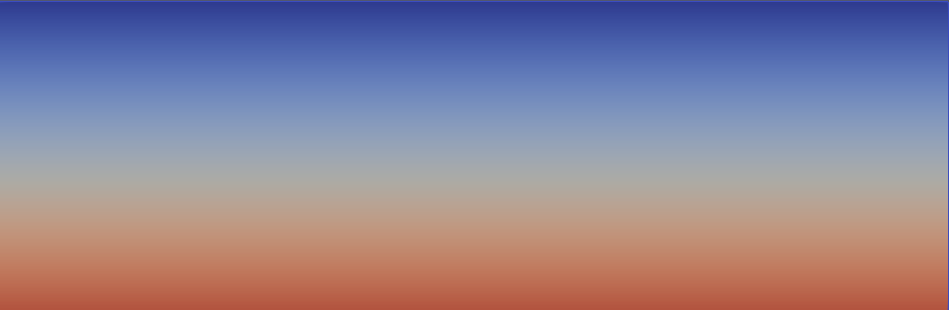
\includegraphics[scale=.3]{animation/fwi_marmousi/fwi_marmousi-00.png}}
            {animation/fwi_marmousi/out.avi}
    \end{center}
  \end{block}

  \begin{block}{Mesh evolution (constant mesh):}
    \begin{center}
      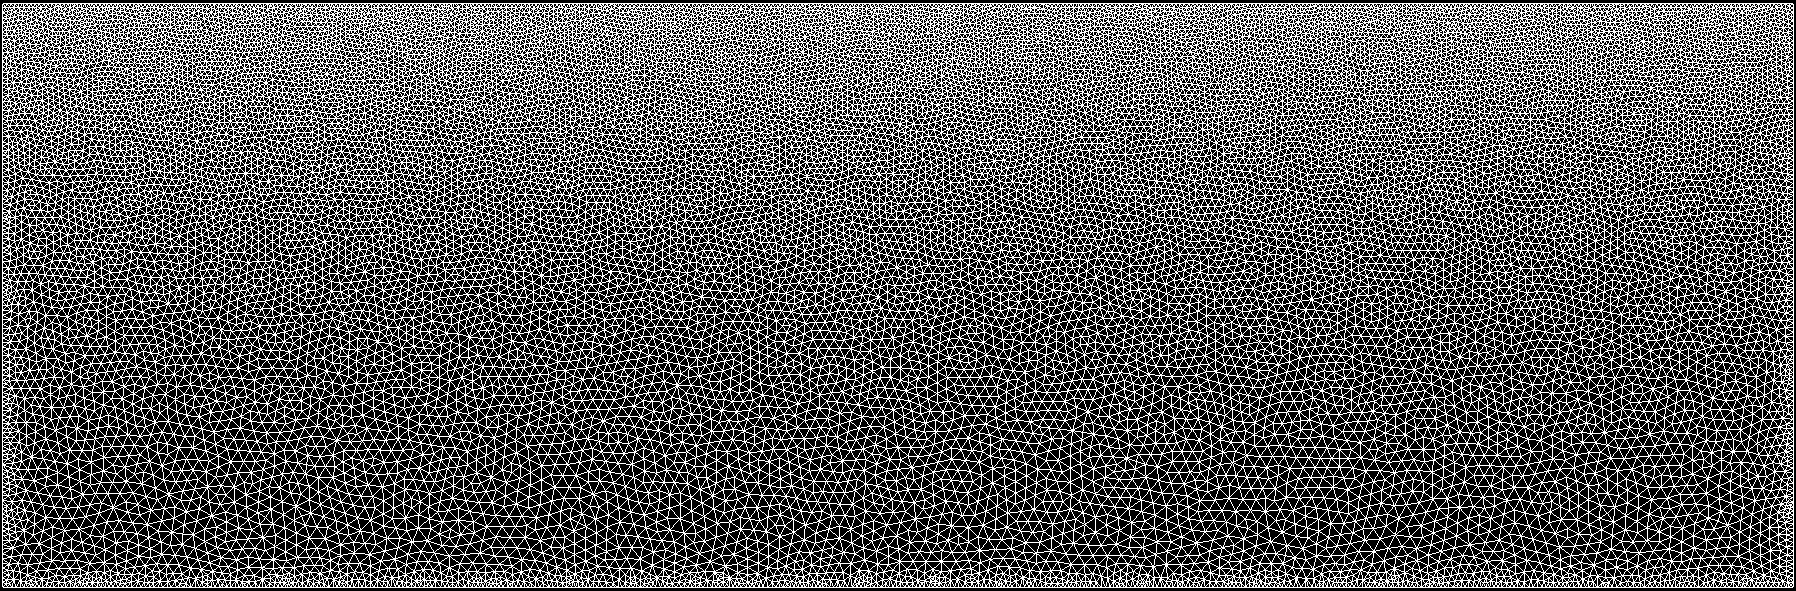
\includegraphics[scale=0.16]{animation/fwi_mesh1_black/fwi_mesh1-00.png}
    \end{center}
  \end{block}

\end{frame}


\begin{frame}[noframenumbering]{Mesh adaptation in FWI workflow}{Motivation:}
  \begin{block}{Model evolution:}
    \begin{center}
      \movie[showcontrols,loop,autostart]
            {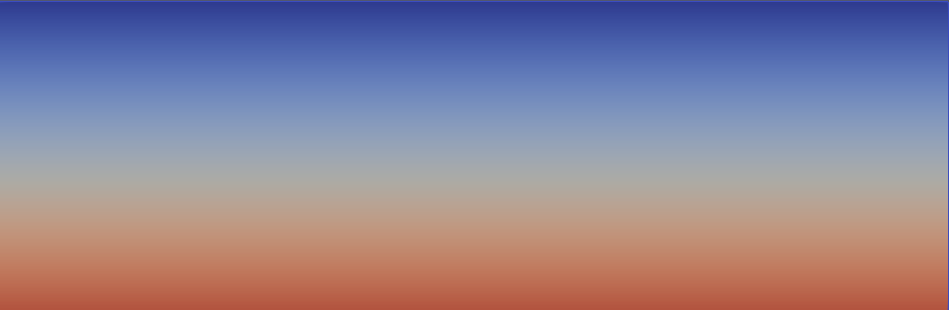
\includegraphics[scale=.3]{animation/fwi_marmousi/fwi_marmousi-00.png}}
            {animation/fwi_marmousi/out.avi}
    \end{center}
  \end{block}

  \begin{block}{Mesh evolution (model adaptative):}
    \begin{center}
            \movie[showcontrols,loop,autostart]
            {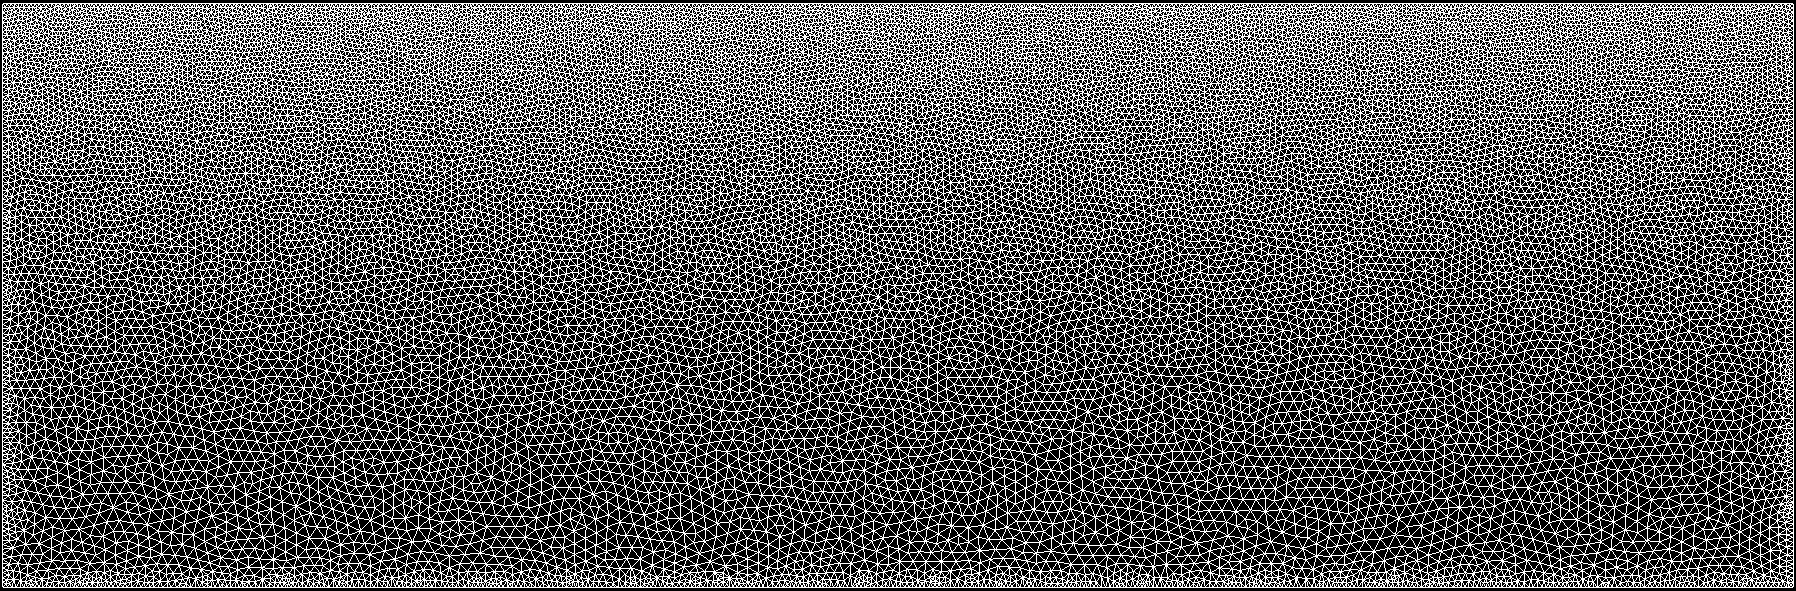
\includegraphics[scale=0.16]{animation/fwi_mesh1_black/fwi_mesh1-00.png}}
            {animation/fwi_mesh1_black/out.avi}
    \end{center}
  \end{block}
\end{frame}


\begin{frame}[noframenumbering]{Mesh adaptation in FWI workflow}{Adaptation to the velocity model}
  \begin{block}{Model evolution:}
    \begin{center}
      \movie[showcontrols,loop,autostart]
            {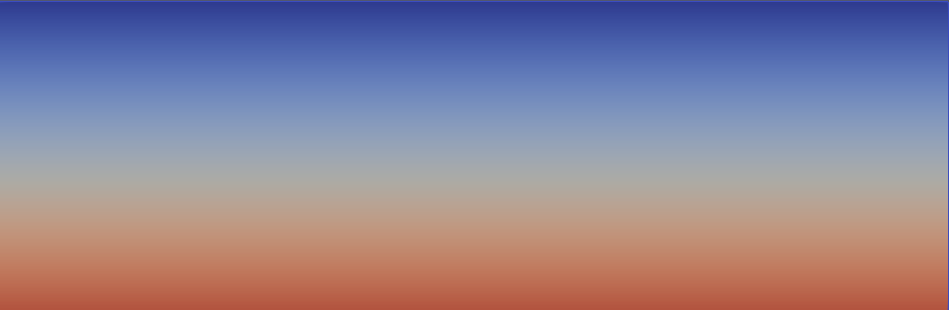
\includegraphics[scale=.3]{animation/fwi_marmousi/fwi_marmousi-00.png}}
            {animation/fwi_marmousi/out.avi}
    \end{center}
  \end{block}

  \begin{block}{Mesh evolution (model and frequency adaptative):}
    \begin{center}
            \movie[showcontrols,loop,autostart]
            {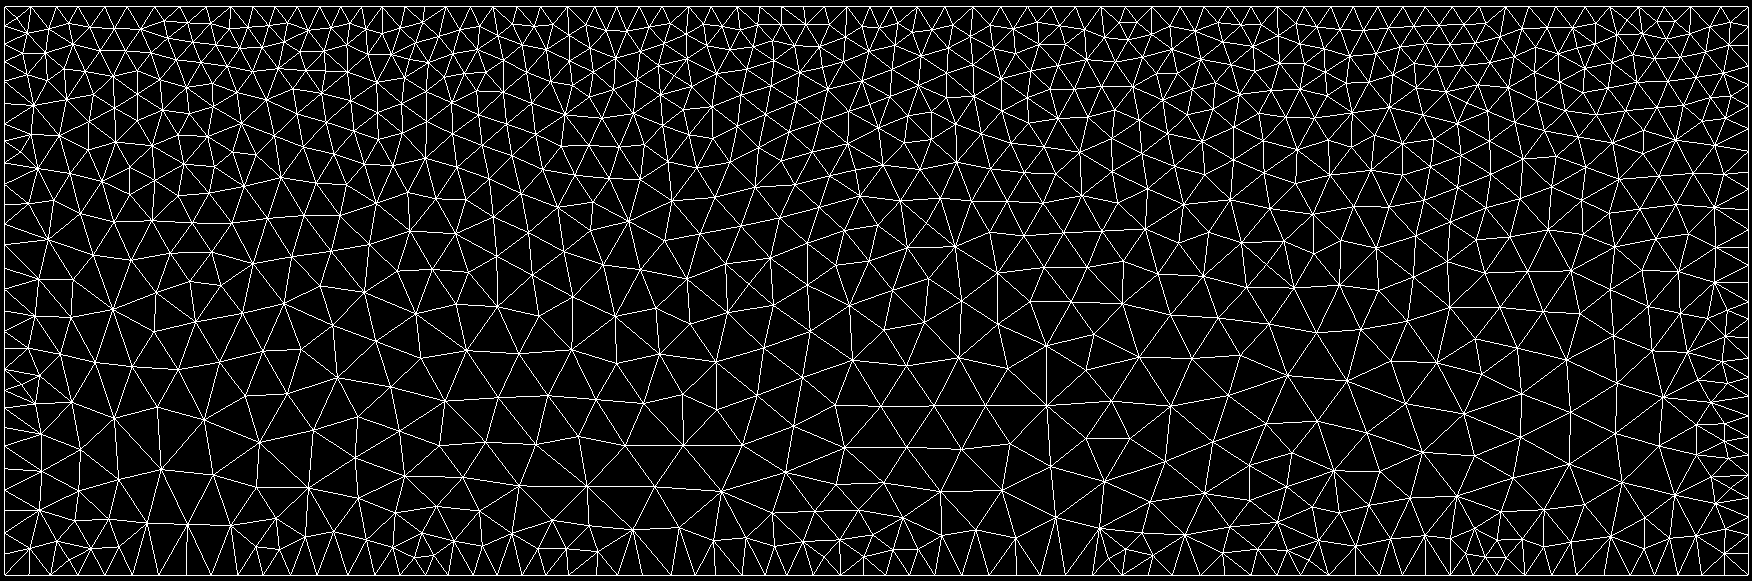
\includegraphics[scale=0.16]{animation/fwi_mesh2/fwi_mesh2-00.png}}
            {animation/fwi_mesh2/out.avi}
    \end{center}
  \end{block}
\end{frame}





% ============================================
% ====== Frame : Introduction Questions  =====
% ============================================


\begin{frame}{Mesh adaptation in FWI workflow}{Introduction}
  Why adapting the mesh in the FWI course ?
  \vspace{1cm}
  \begin{itemize}
  \item<2->{Adjust the computational burden}
  \item<3->{ Capture appearing structures}
  \item<4->{Avoid small cells in high velocity structures (\textbf{relax the CFL condition})}
  \item<5->{Enables to choose the mesh according to the frequency range currently reconstructed}
  \end{itemize}
\end{frame}



% ============================================
% ====== Frame : Proposition Ajout FWI  ======
% ============================================

\begin{frame}{Mesh adaptation in FWI workflow}{Introduction}
  How to include mesh adaptation into FWI workflow ?
\begin{figure}[!htbp]
\centering
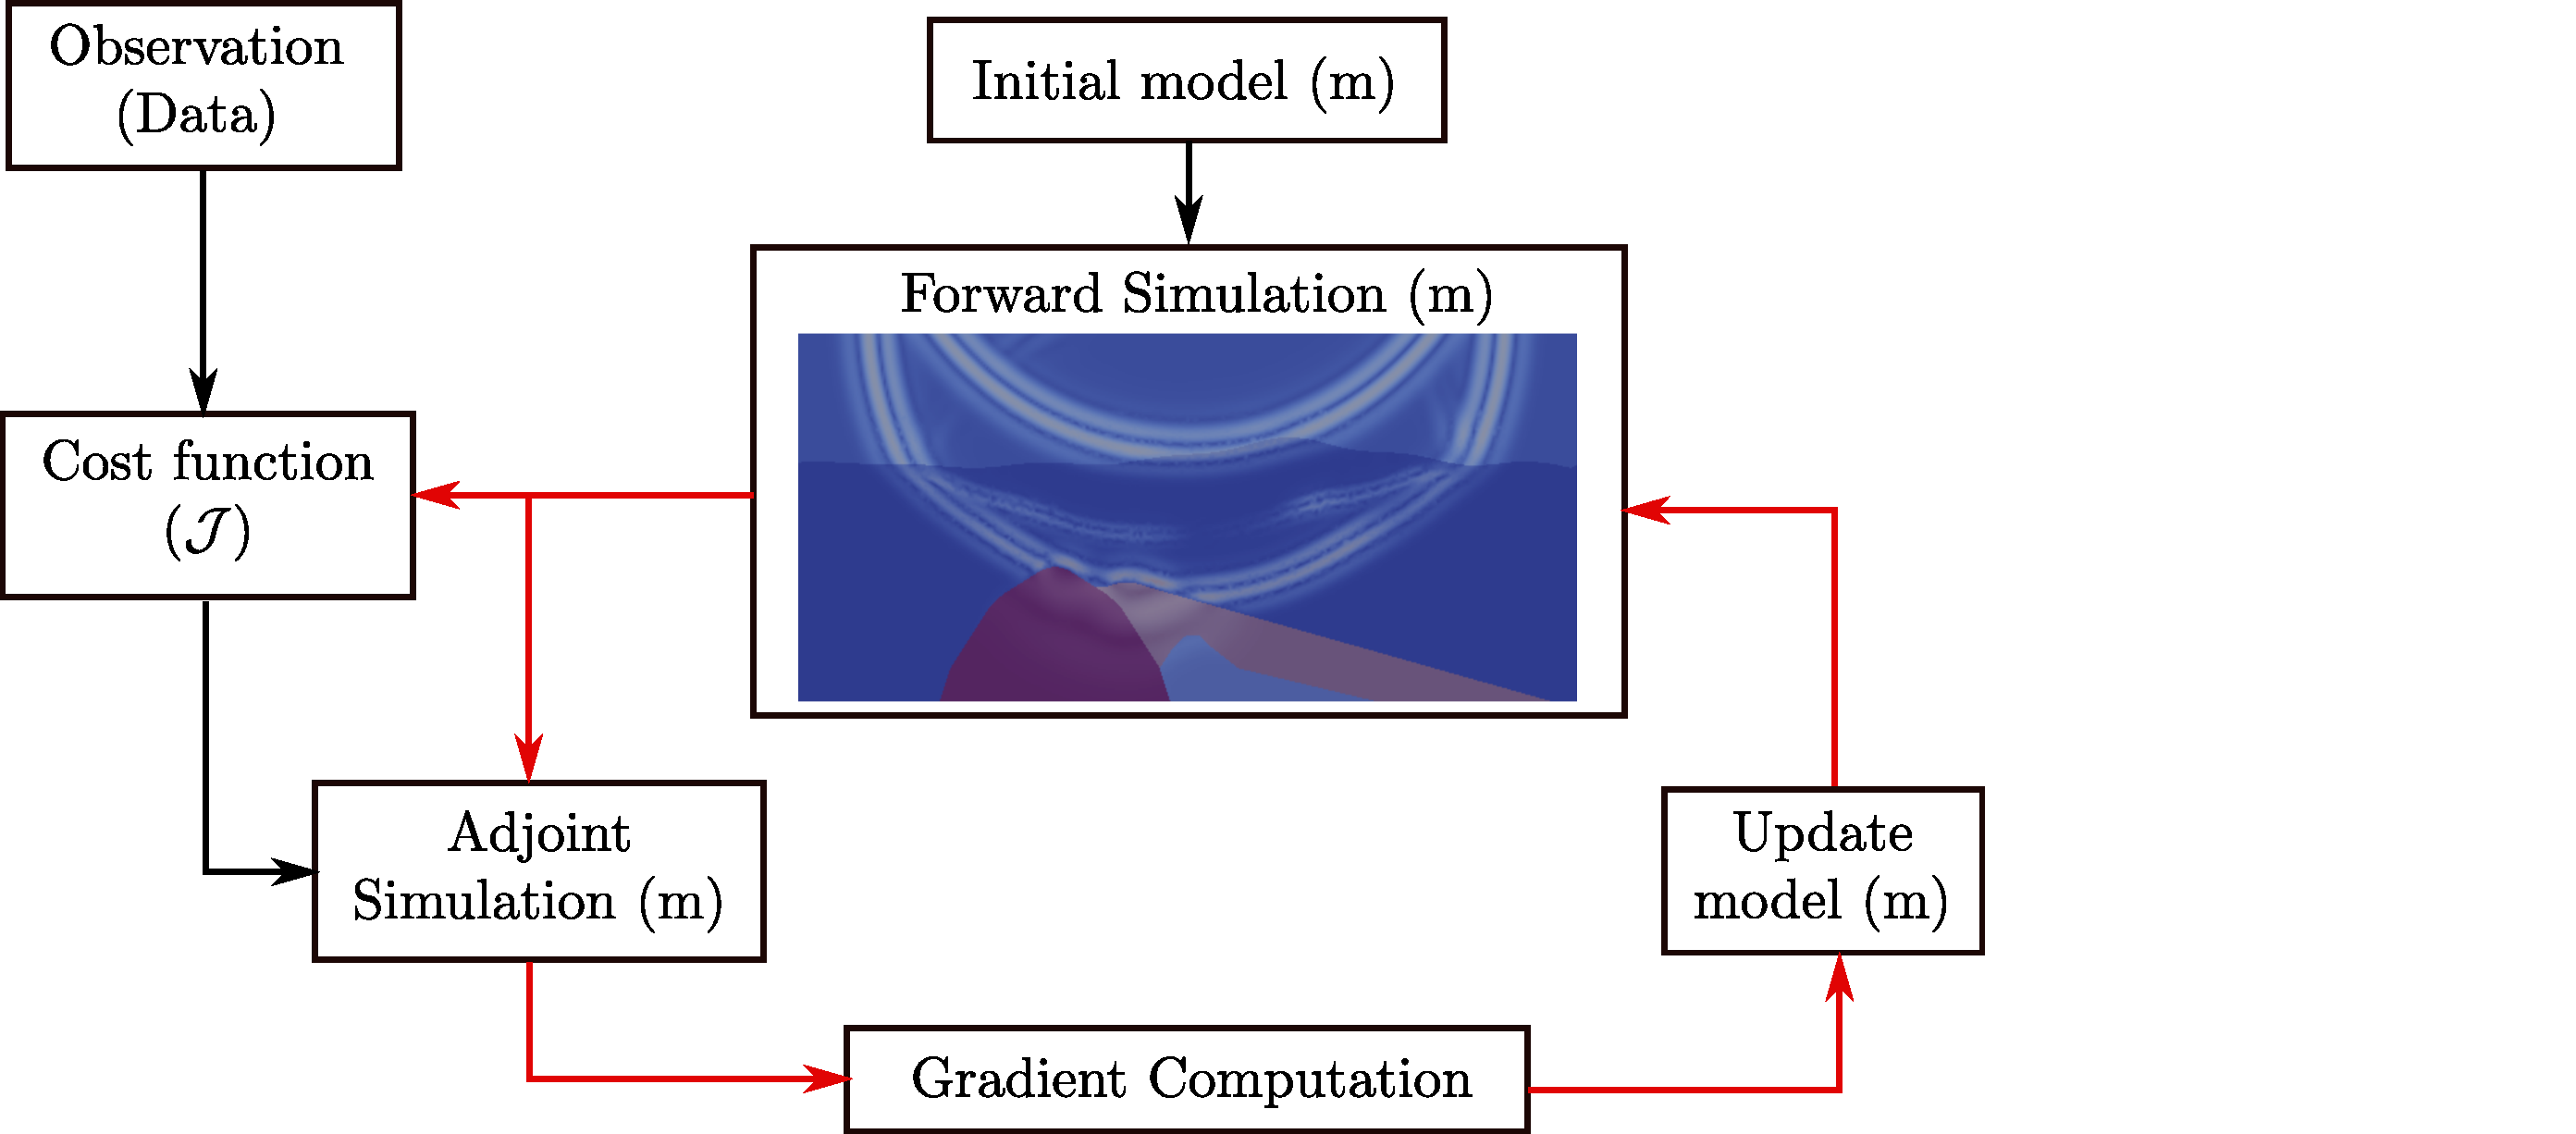
\includegraphics[scale=0.2]{image/fwi_workflow_mesh_adapt0.pdf}
\caption{FWI workflow extended with mesh adaptation.}
\label{fwi_workflow_mesh_extended}
\end{figure}
\end{frame}


\begin{frame}[noframenumbering]{Mesh adaptation in FWI workflow}{Introduction}
  How to include mesh adaptation into FWI workflow ?
\begin{figure}[!htbp]
\centering
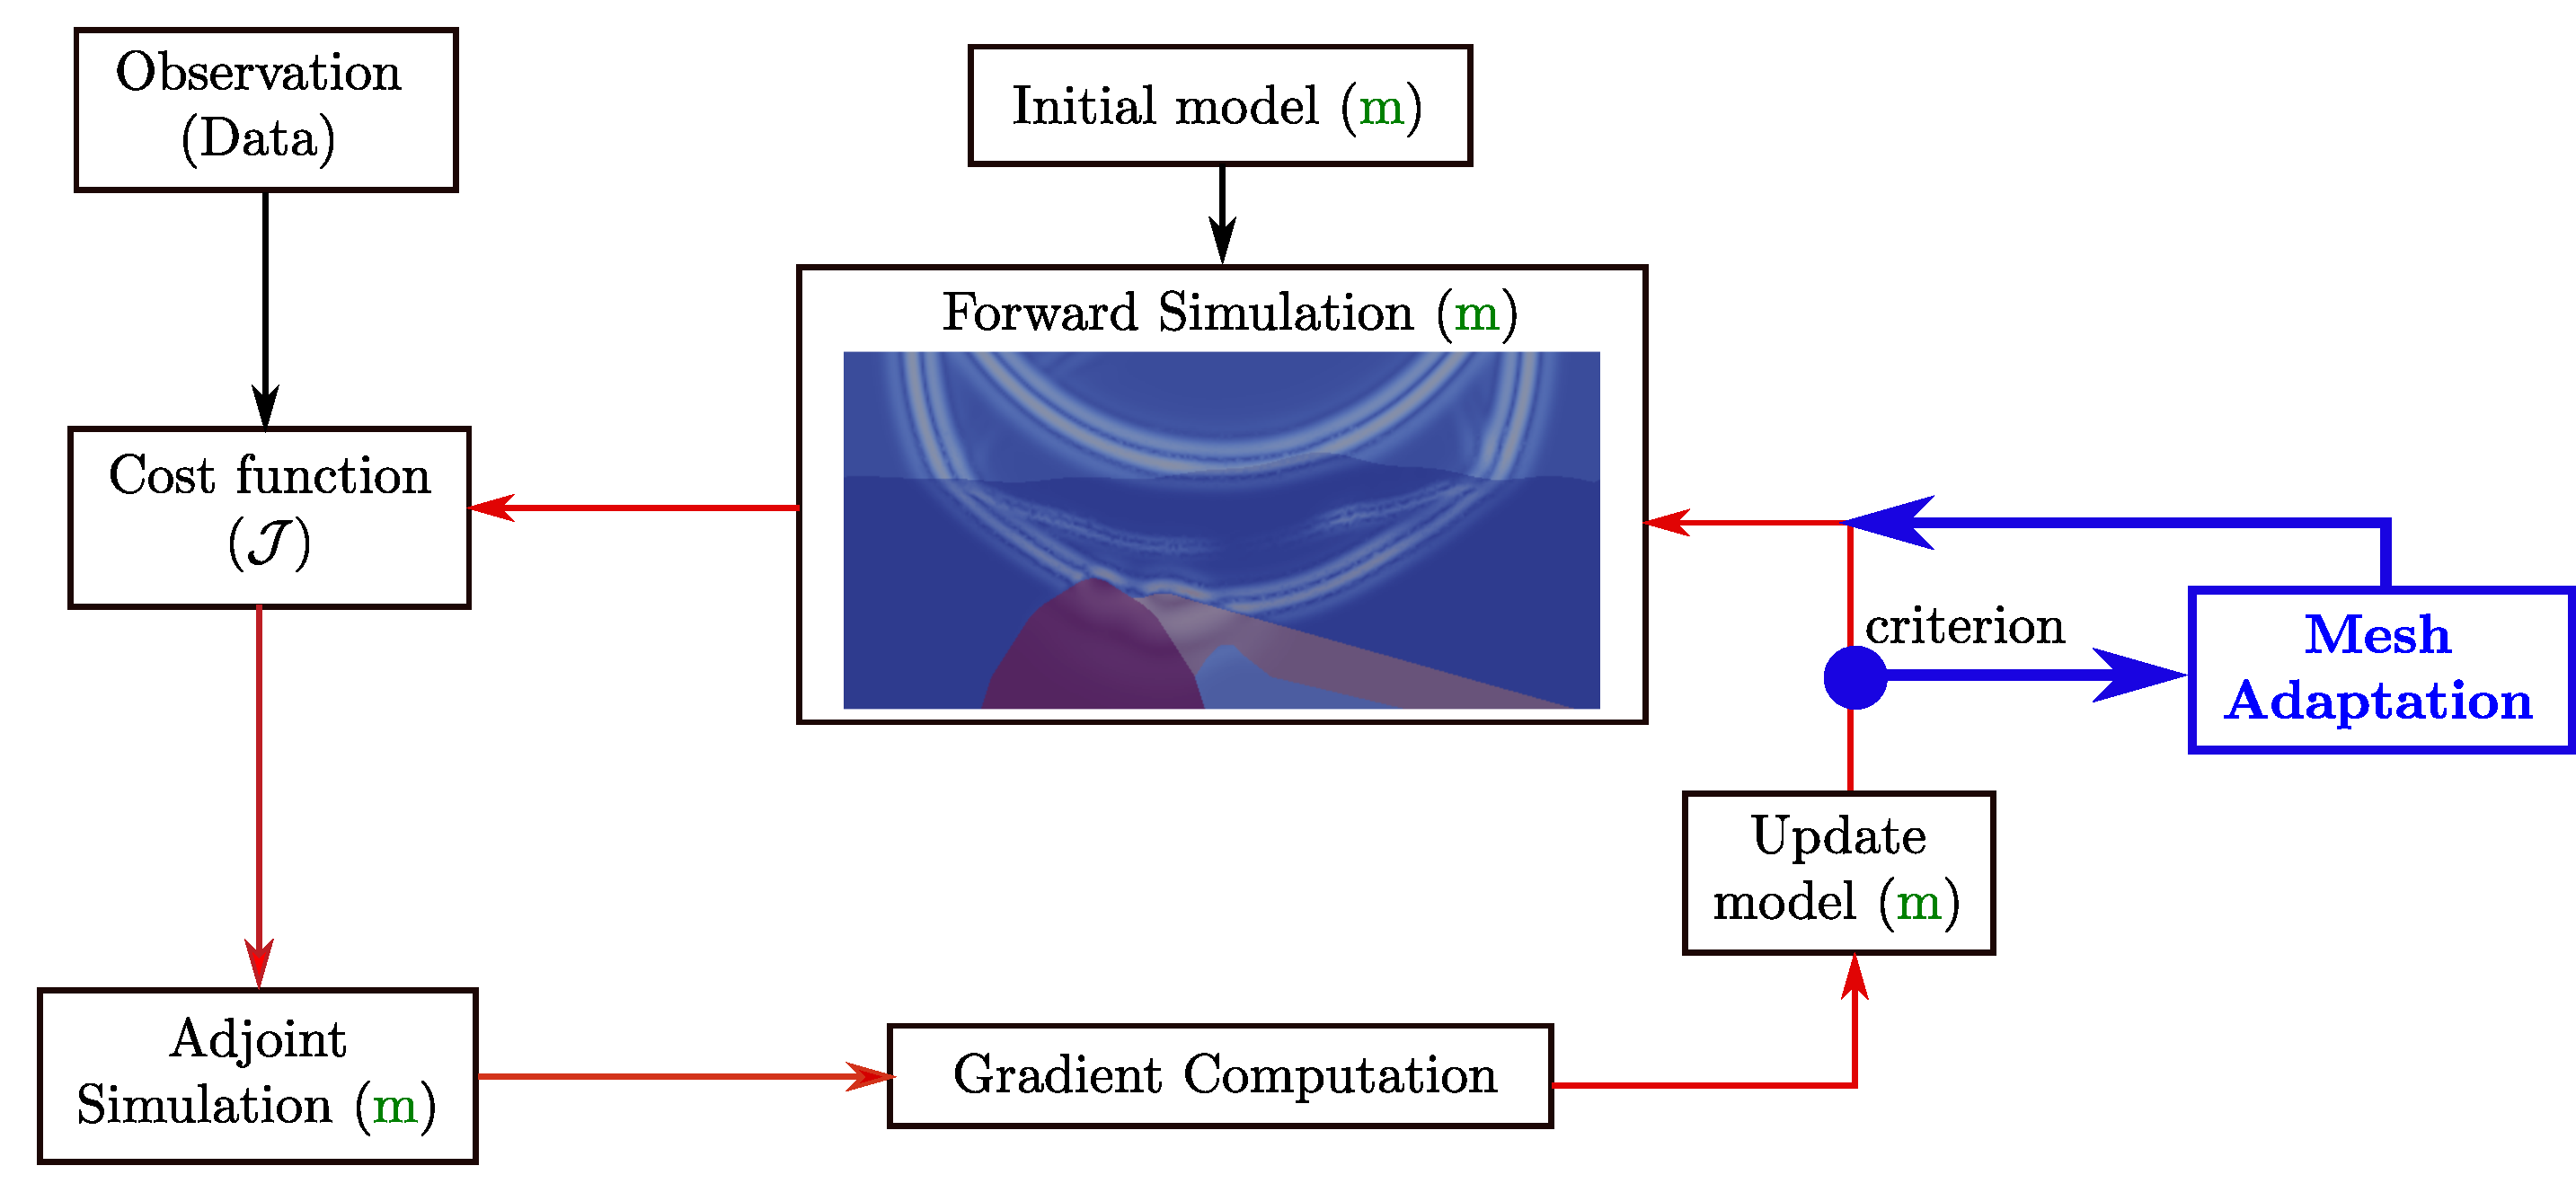
\includegraphics[scale=0.2]{image/fwi_workflow_mesh_adapt.pdf}
\caption{FWI workflow extended with mesh adaptation.}
\label{fwi_workflow_mesh_extended}
\end{figure}
\end{frame}



% =========================================================
% ====== Frame : Mesh adaptation classical workflow  ======
% =========================================================

\setbeamercovered{invisible}
\subsection{Mesh Adaptation principle}

\begin{frame}{Mesh Adaptation}{Definitions}
  $\boldsymbol{S^i}$ : solution at the $i^{th}$ iteration |
  $\boldsymbol{\Triangles^i}$ : mesh at the $i^{th}$ iteration
  \vspace{0.5cm}
   \begin{figure}
     \begin{tikzpicture}
       \node[anchor=south west,inner sep=0] at (0,0) {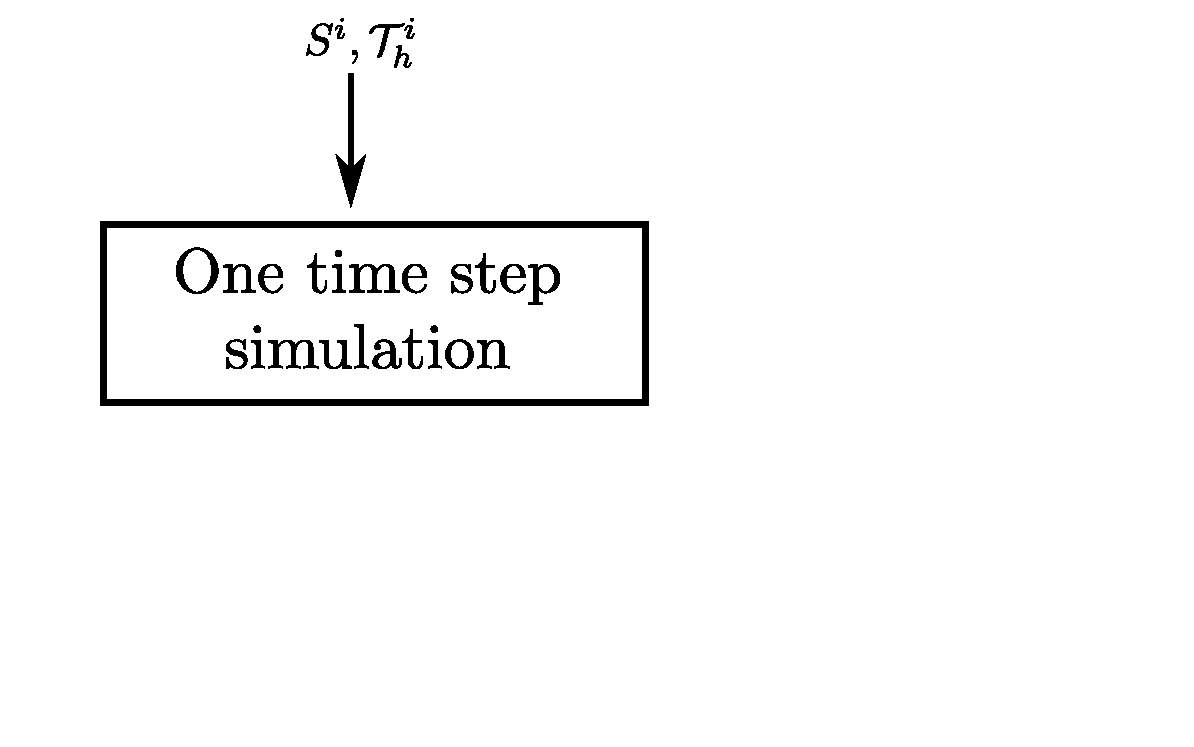
\includegraphics[width=0.8\textheight]{image/mesh_adapt_workflow5.pdf}};
        \end{tikzpicture}
        \caption{Classical mesh adaptation workflow.}
   \end{figure}
\end{frame}


\begin{frame}[noframenumbering]{Mesh Adaptation}{Definitions}
  $\boldsymbol{S^i}$ : solution at the $i^{th}$ iteration |
  $\boldsymbol{\Triangles^i}$ : mesh at the $i^{th}$ iteration
  \vspace{0.5cm}
   \begin{figure}
     \begin{tikzpicture}
       \node[anchor=south west,inner sep=0] at (0,0) {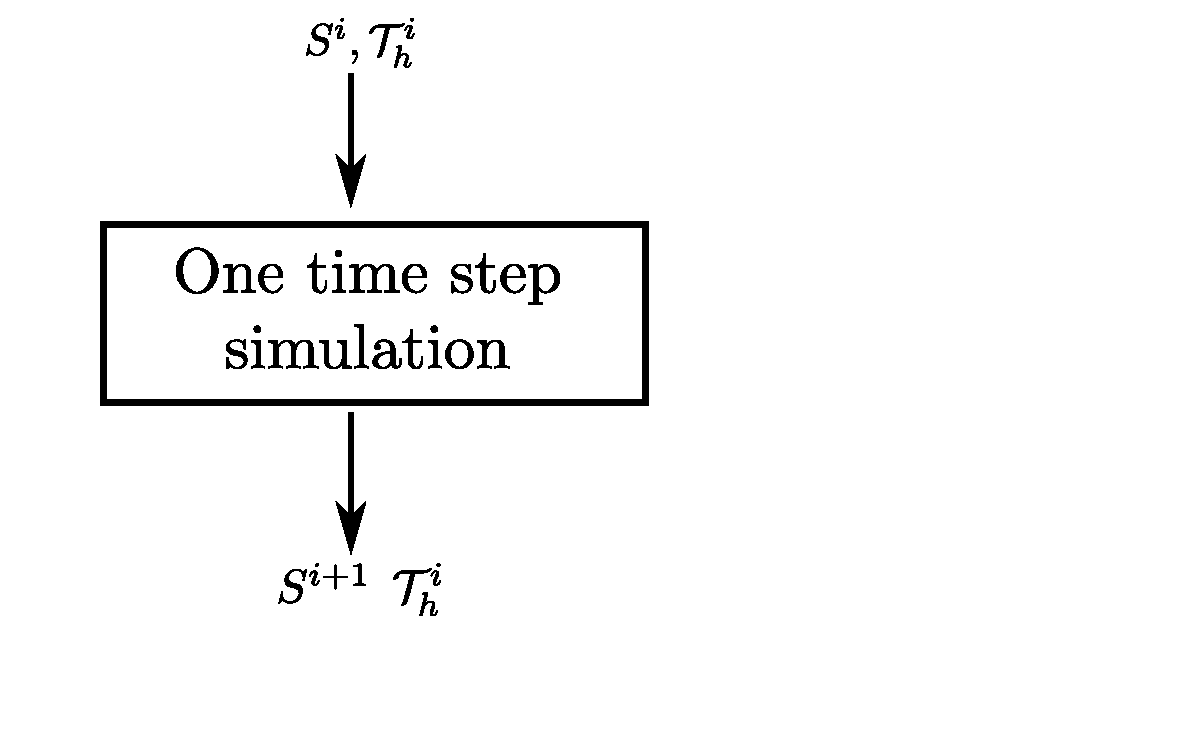
\includegraphics[width=0.8\textheight]{image/mesh_adapt_workflow4.pdf}};
        \end{tikzpicture}
        \caption{Classical mesh adaptation workflow.}
   \end{figure}
\end{frame}


\begin{frame}[noframenumbering]{Mesh Adaptation}{Definitions}
  $\boldsymbol{S^i}$ : solution at the $i^{th}$ iteration |
  $\boldsymbol{\Triangles^i}$ : mesh at the $i^{th}$ iteration
  \vspace{0.5cm}
   \begin{figure}
     \begin{tikzpicture}
       \node[anchor=south west,inner sep=0] at (0,0) {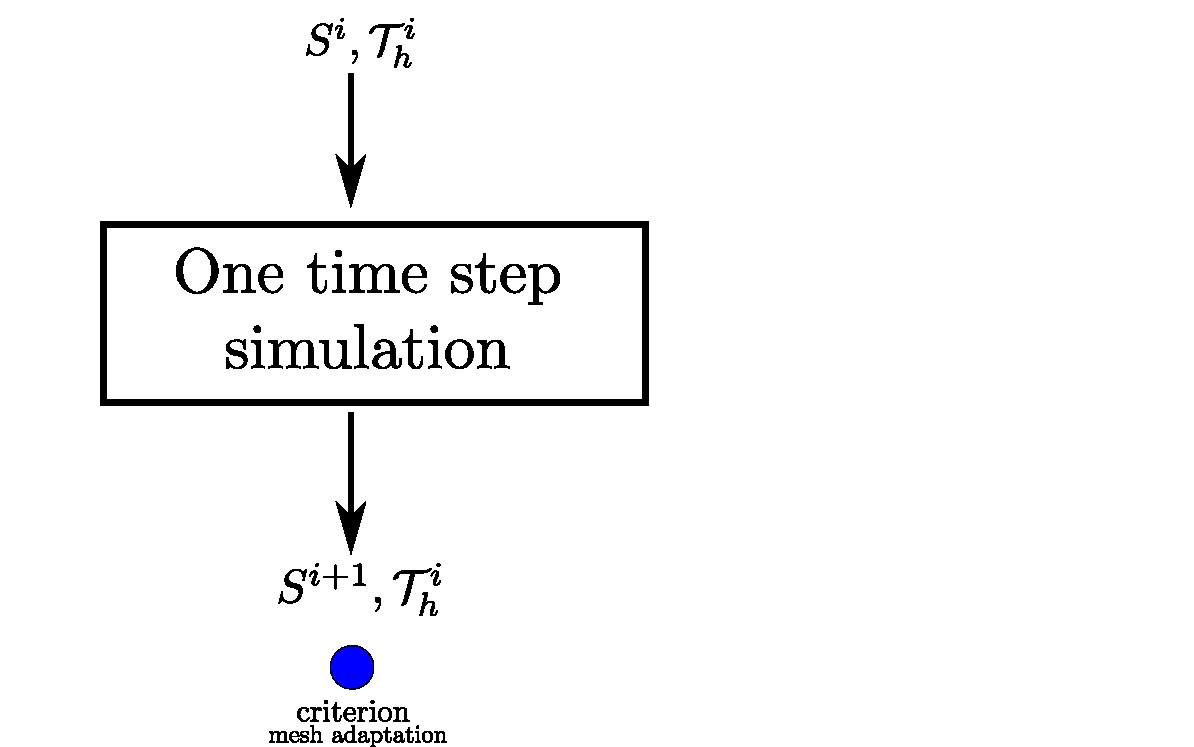
\includegraphics[width=0.8\textheight]{image/mesh_adapt_workflow3.pdf}};
        \end{tikzpicture}
        \caption{Classical mesh adaptation workflow.}
   \end{figure}
\end{frame}


\begin{frame}[noframenumbering]{Mesh Adaptation}{Definitions}
  $\boldsymbol{S^i}$ : solution at the $i^{th}$ iteration |
  $\boldsymbol{\Triangles^i}$ : mesh at the $i^{th}$ iteration
  \vspace{0.5cm}
   \begin{figure}
     \begin{tikzpicture}
       \node[anchor=south west,inner sep=0] at (0,0) {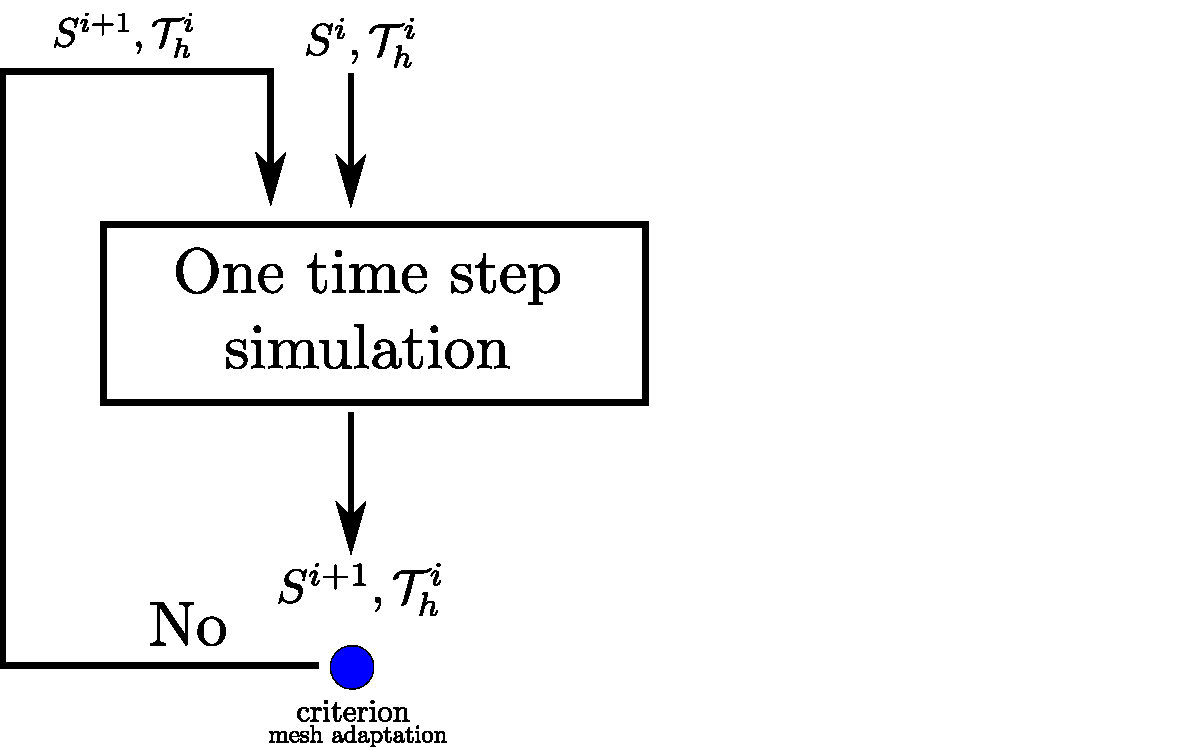
\includegraphics[width=0.8\textheight]{image/mesh_adapt_workflow2.pdf}};
        \end{tikzpicture}
        \caption{Classical mesh adaptation workflow.}
   \end{figure}
\end{frame}


\begin{frame}[noframenumbering]{Mesh Adaptation}{Definitions}
  $\boldsymbol{S^i}$ : solution at the $i^{th}$ iteration |
  $\boldsymbol{\Triangles^i}$ : mesh at the $i^{th}$ iteration
  \vspace{0.5cm}
   \begin{figure}
     \begin{tikzpicture}
       \node[anchor=south west,inner sep=0] at (0,0) {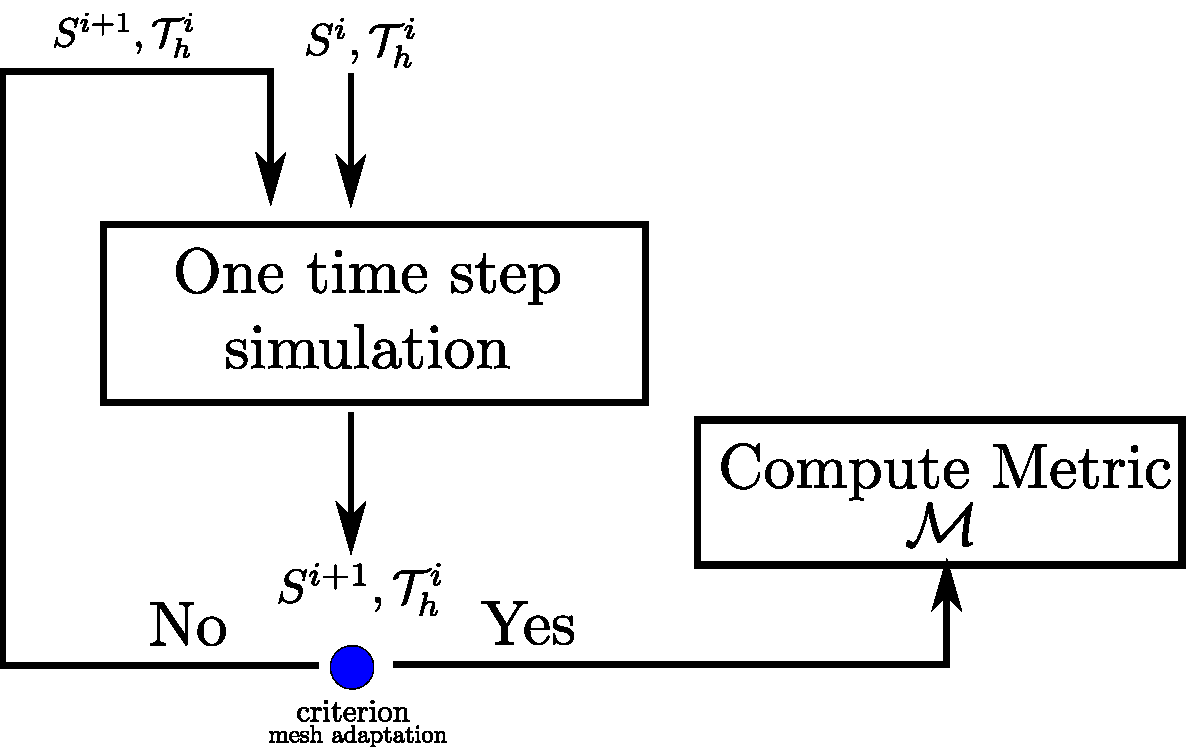
\includegraphics[width=0.8\textheight]{image/mesh_adapt_workflow1.pdf}};
        \end{tikzpicture}
        \caption{Classical mesh adaptation workflow.}
   \end{figure}
\end{frame}


\begin{frame}[noframenumbering]{Mesh Adaptation}{Definitions}
  $\boldsymbol{S^i}$ : solution at the $i^{th}$ iteration |
  $\boldsymbol{\Triangles^i}$ : mesh at the $i^{th}$ iteration
  \vspace{0.5cm}
   \begin{figure}
     \begin{tikzpicture}
       \node[anchor=south west,inner sep=0] at (0,0) {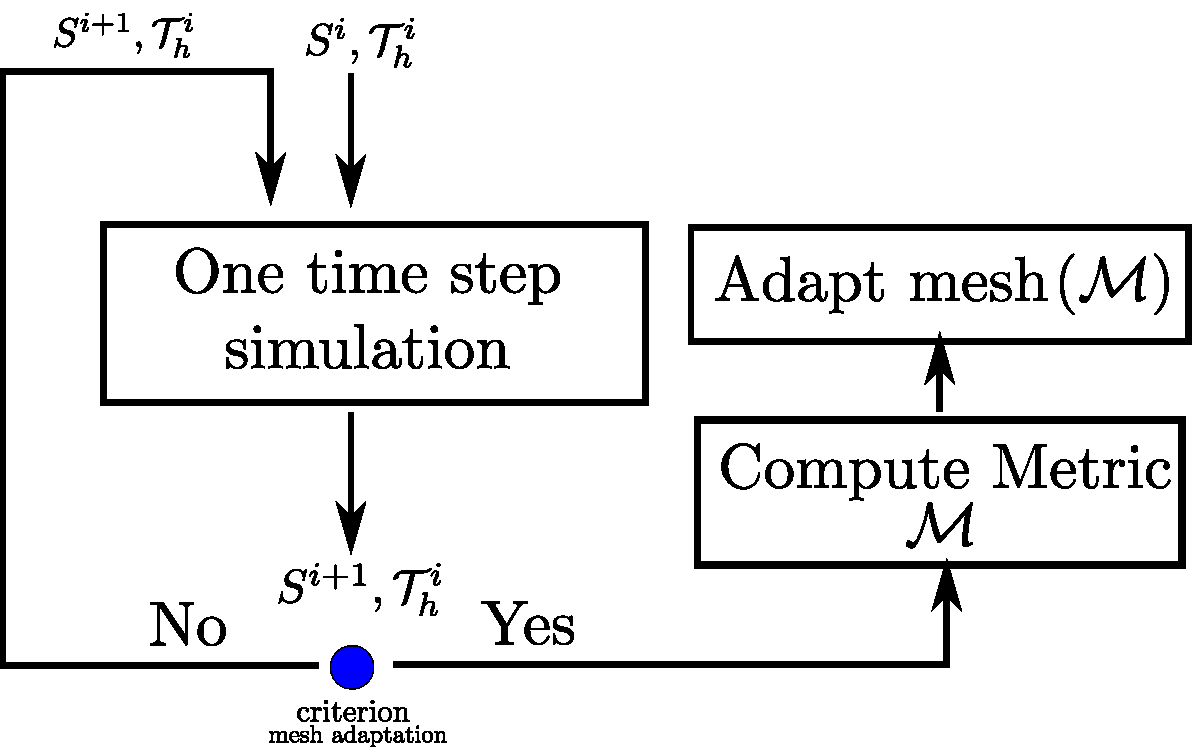
\includegraphics[width=0.8\textheight]{image/mesh_adapt_workflow6.pdf}};
        \end{tikzpicture}
        \caption{Classical mesh adaptation workflow.}
   \end{figure}
\end{frame}


\begin{frame}[noframenumbering]{Mesh Adaptation}{Definitions}

  $\boldsymbol{S^i}$ : solution at the $i^{th}$ iteration |
  $\boldsymbol{\Triangles^i}$ : mesh at the $i^{th}$ iteration

  \vspace{0.5cm}
   \begin{figure}
     \begin{tikzpicture}
       \node[anchor=south west,inner sep=0] at (0,0) {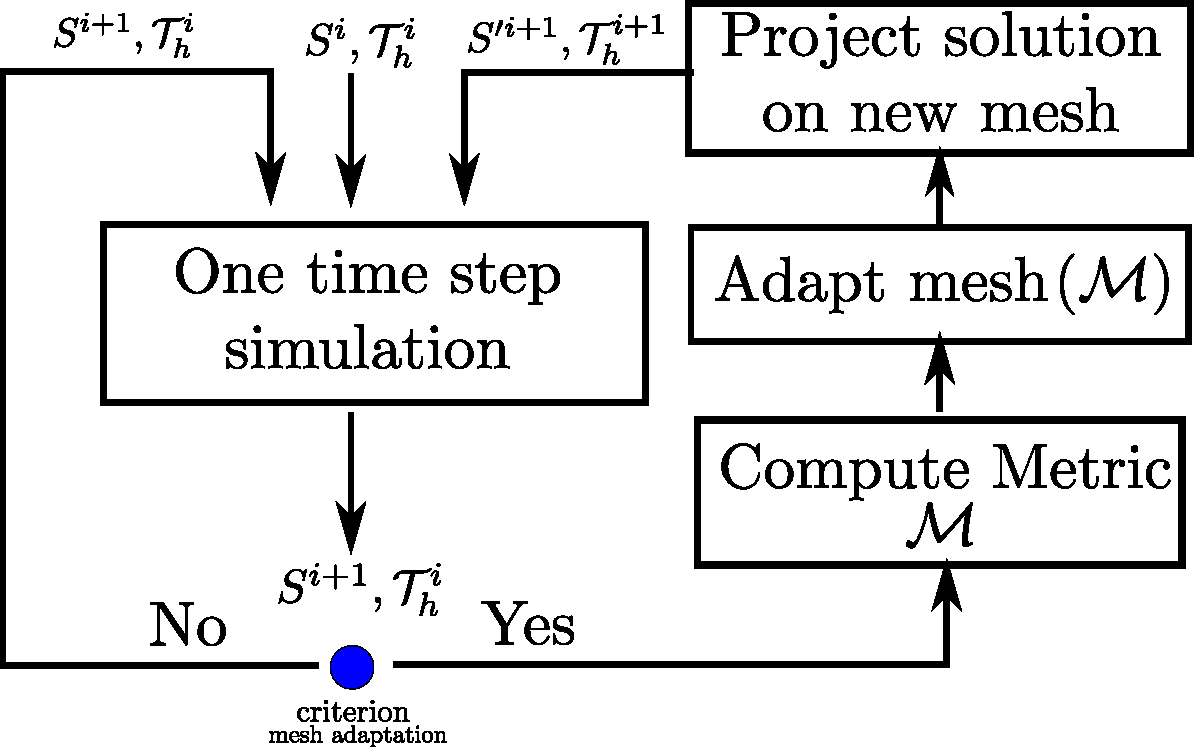
\includegraphics[width=0.8\textheight]{image/mesh_adapt_workflow.pdf}};
        \uncover<2->{
        \node at (8.0,1.52) {\textbf{\textcolor{blue}{Mshmet \footcite{Mshmet}}}};
        \node at (7.8,2.64) {\textbf{\textcolor{red}{MMG \footcite{Mmg}}}};
          \draw [blue,ultra thick,rounded corners] (3.9,0.95) rectangle (6.95,2.0);
          \draw [red,ultra thick,rounded corners] (3.9,2.25) rectangle (6.95,3.1);}
        \end{tikzpicture}
        \caption{Classical mesh adaptation workflow.}
   \end{figure}
\end{frame}








% ============================================
% ====== Frame : Some definitiions      ======
% ============================================

\begin{frame}{Some Definitions}
  \vspace{-0.1cm}
  \uncover<2->{
  \begin{block}{Metric definition:}
    \small
    $\forall P \in \Domain, \boldsymbol{\metric(P)}$ is a \textbf{SPD matrix} of size $\dim \times \dim$.

      \begin{empheq}{align}
    \forall (P,M) \in \Domain^2, \parallel\vec{PM} \parallel^2_{\metric(P)} &= \langle \vec{PM}, \metric(P) \vec{PM} \rangle \\
                              %\parallel\vec{PM} \parallel_{\metric(P)}   &= \sqrt{\vec{PM}^\top \metric(P) \vec{PM}}
      \end{empheq}
      \end{block}
}
  \uncover<3->{
    \vspace{-0.1cm}
  \begin{block}{Unit ball : Set of point $M$ such that $\parallel \vec{PM} \parallel_{\metric(P)} = 1.$}
    \small
          \begin{empheq}{align}
   \text{In 2D :  } \metric(P) = S \Lambda S^\top\,, \Lambda =  \begin{pmatrix}
    \lambda_{1} &\\
    & \lambda_2
  \end{pmatrix}\,, \lambda_1 \geq \lambda_2 > 0.
          \end{empheq}
          \begin{multicols}{2}
            \begin{figure}[!htbp]
\centering
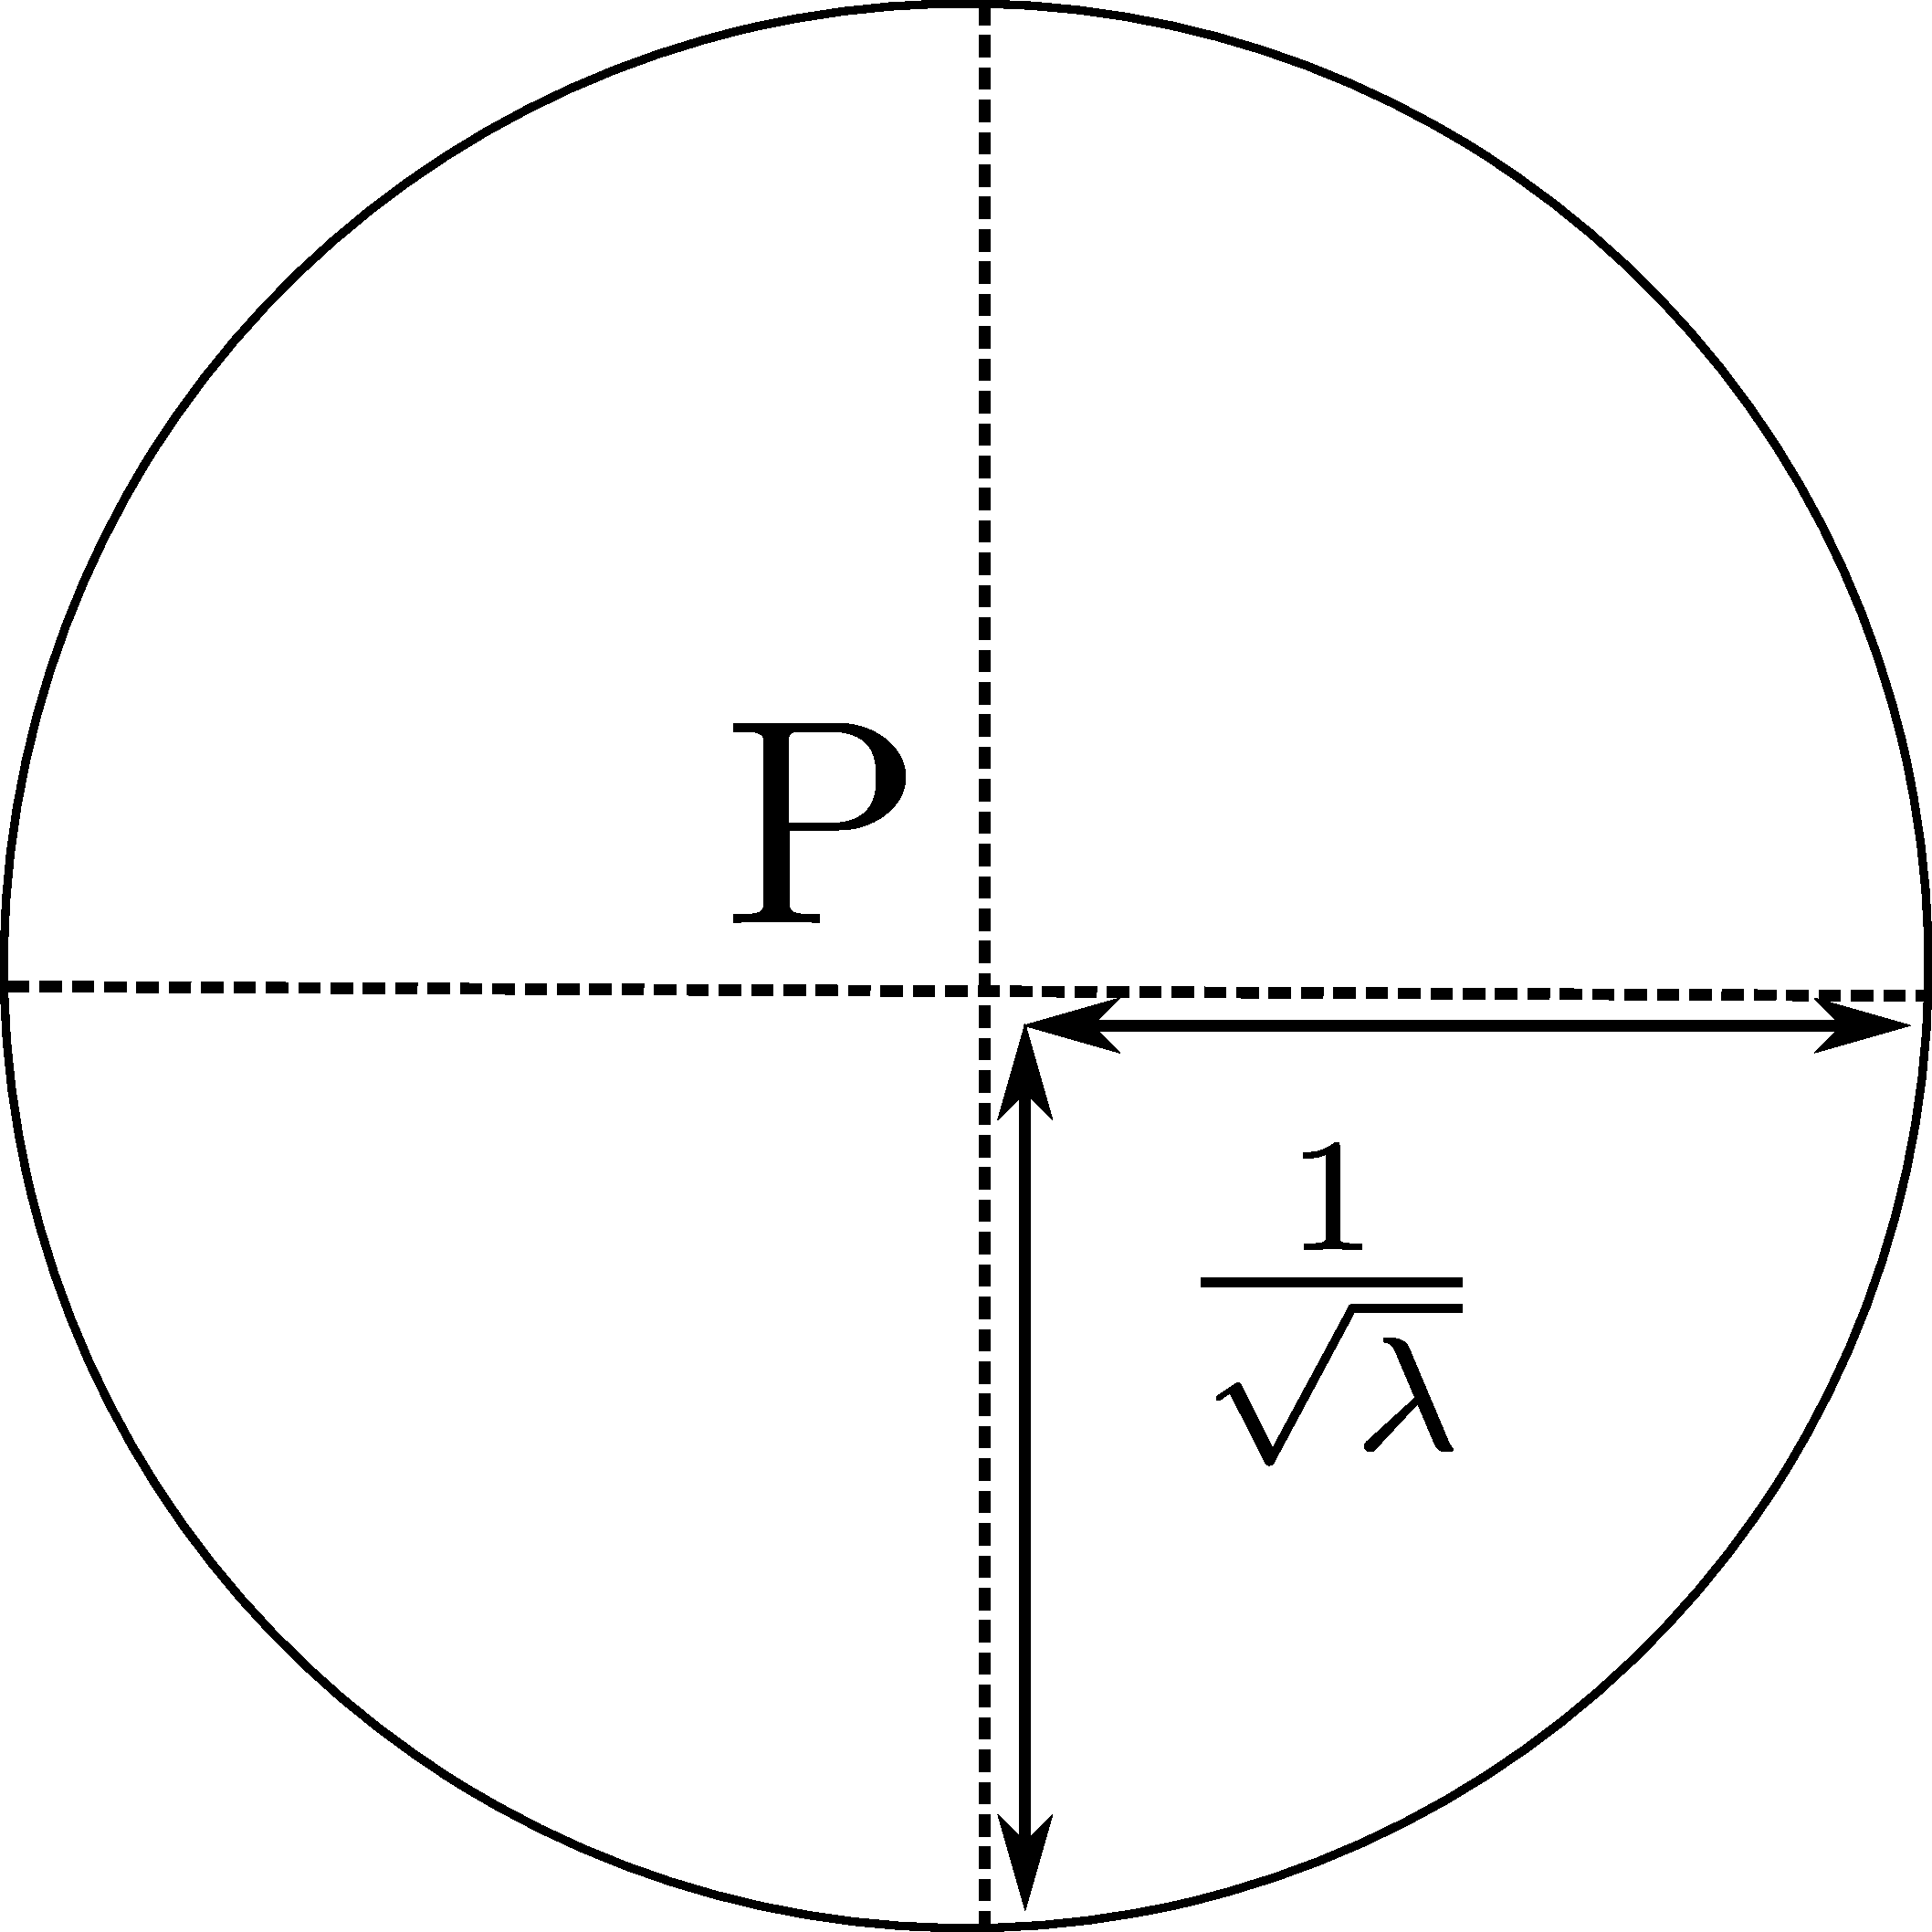
\includegraphics[scale=0.04]{image/ellipse_iso_triangle.pdf}
\vspace{0.2cm}
\caption{\tiny{Unit ball $(\lambda_1 = \lambda_2 = \lambda)$}}
\label{ellipse_iso_triangle}
\end{figure}
            \columnbreak
           \begin{figure}[!htbp]
\centering
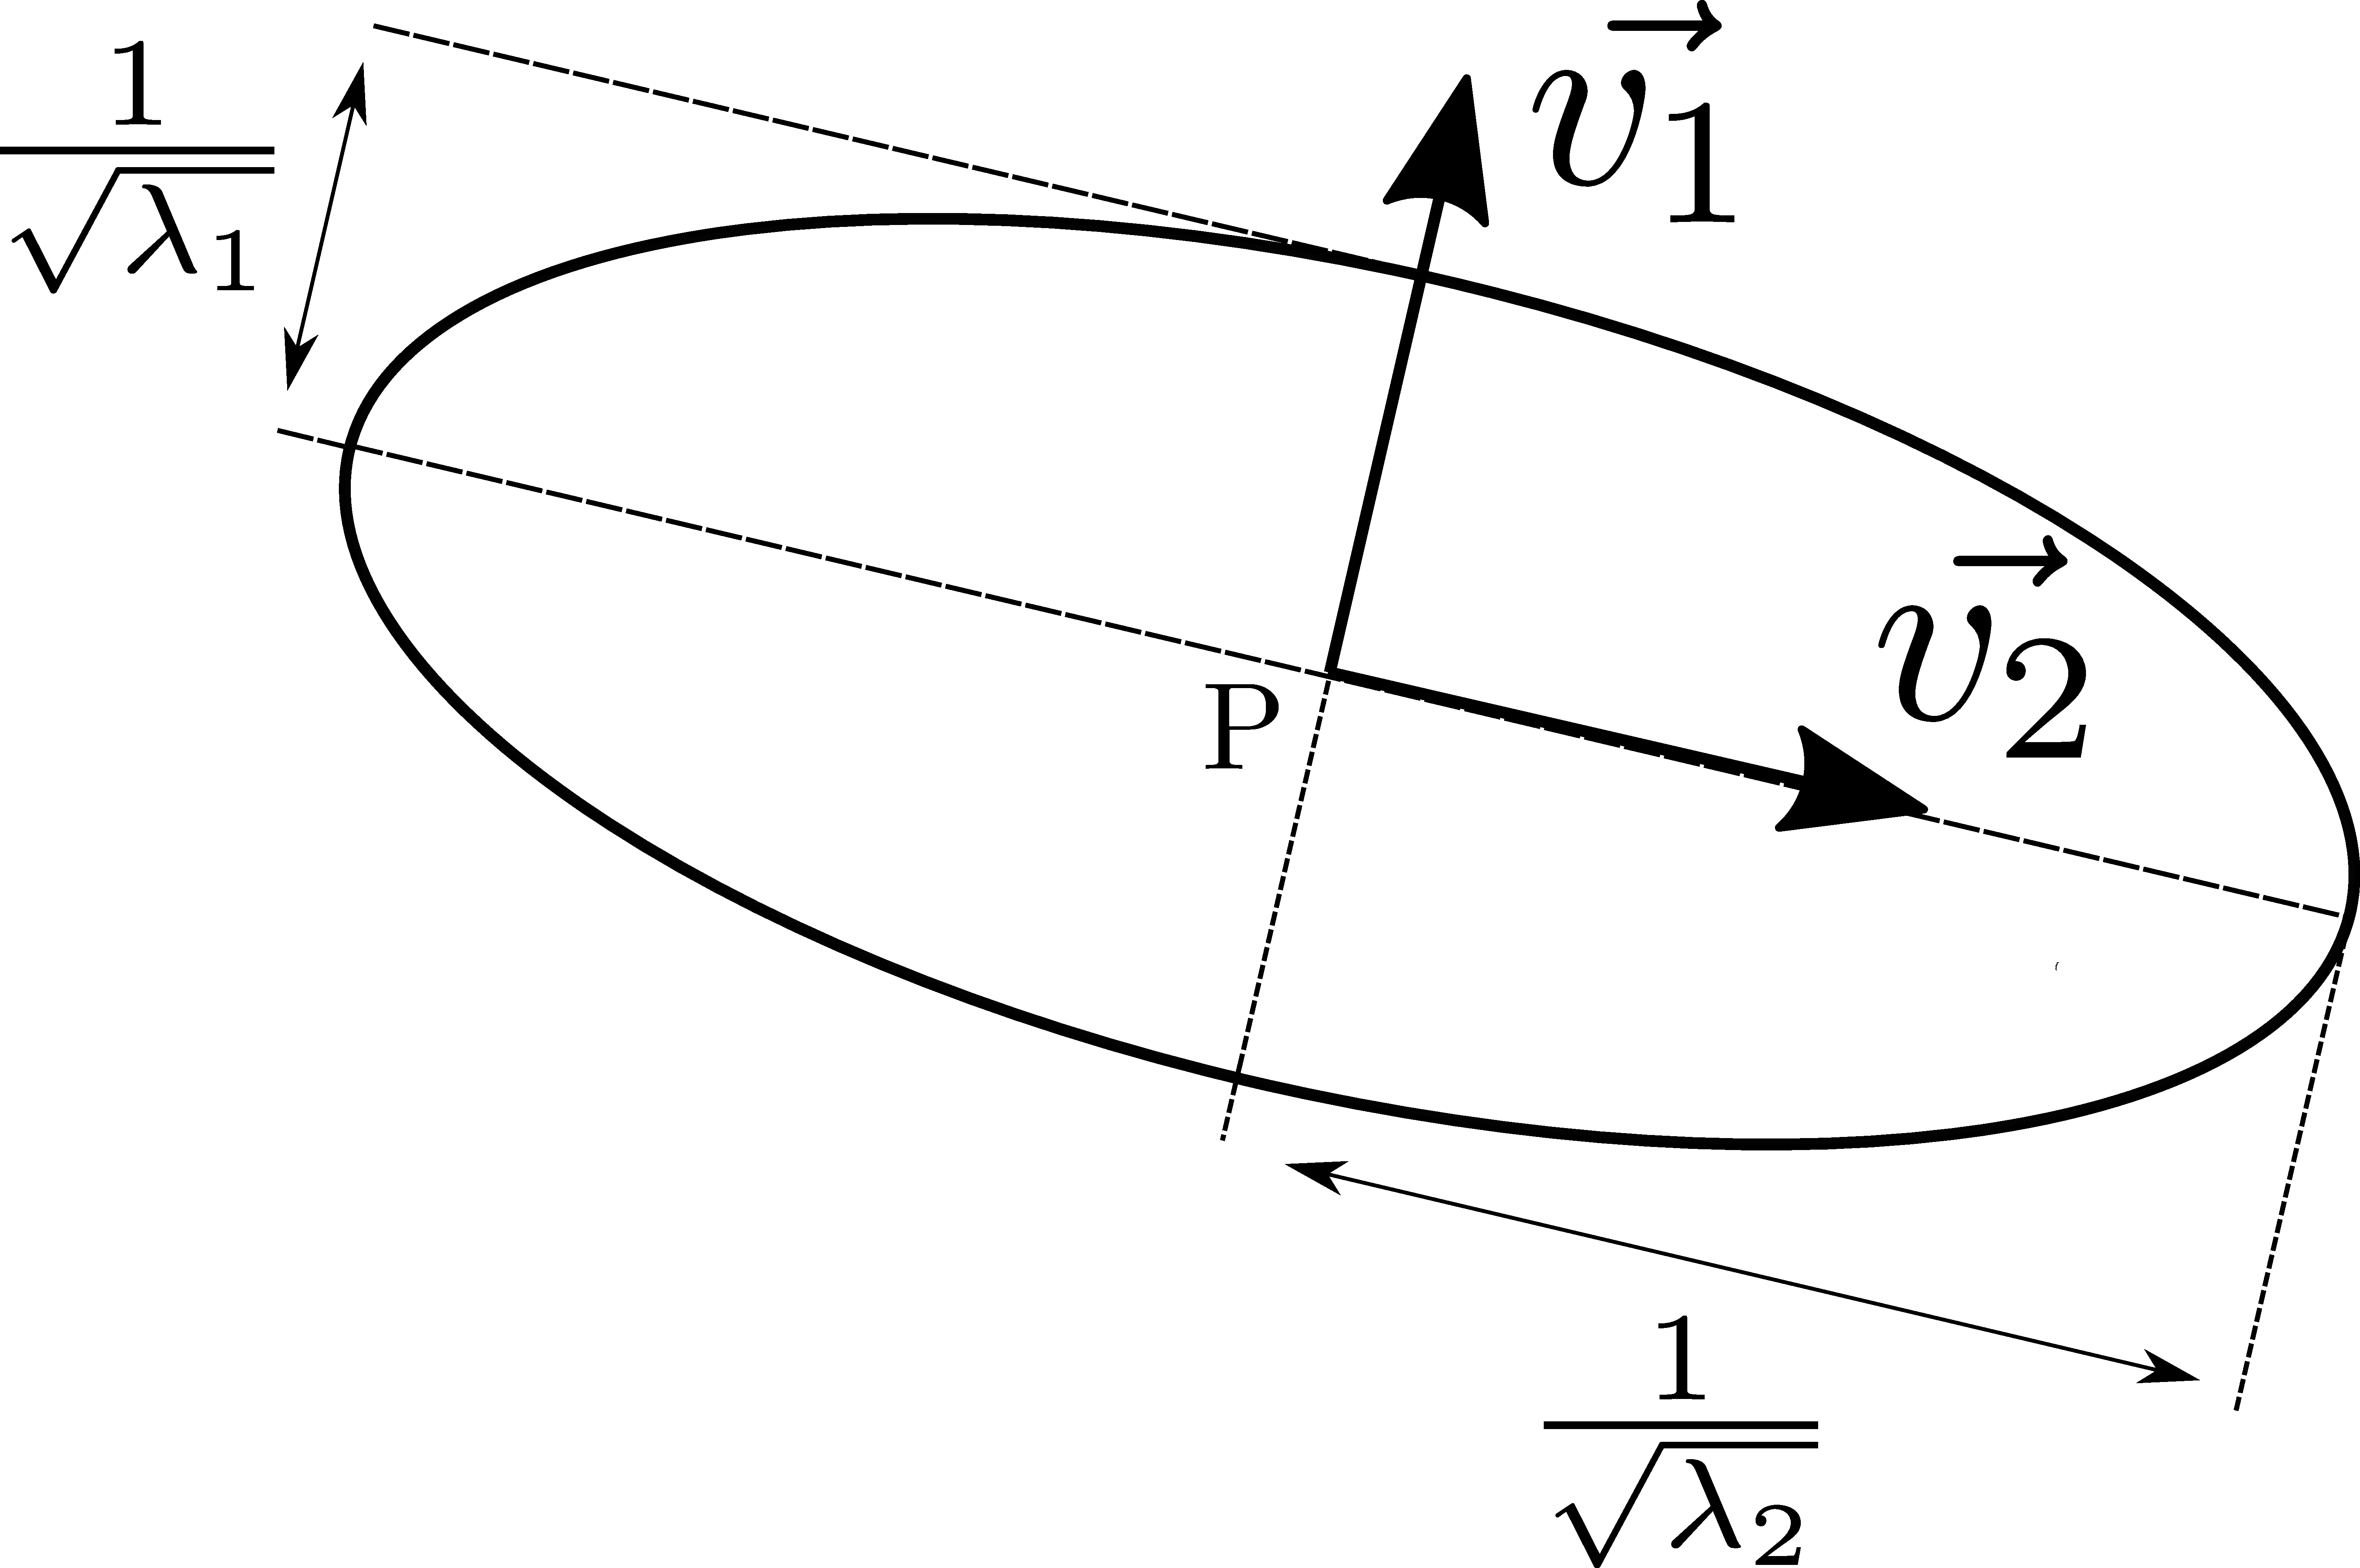
\includegraphics[scale=0.028]{image/ellipse_aniso.pdf}
\vspace{-0.3cm}
\caption{\tiny{Unit ball $(\lambda_1 >> \lambda_2)$}}
\label{ellipse_iso_triangle}
     \end{figure}
 \end{multicols}
  \end{block}
  }
\end{frame}




% ============================================
% ====== Frame : Control the error      ======
% ============================================

\begin{frame}{Control the interpolation error}
  \small
  [P.J. Frey and F. Alauzet]\footcite{freyAnisotropicMeshAdaptation2005}: control the error on the element $\element$:
\vspace{-0.1cm}
  \begin{multicols}{2}
  \begin{empheq}{align}
\exists \, \bar{\metric}(\element)\, / \, \varepsilon_\element = \underset{\overrightarrow{e}\in E_\element}{max} \langle \overrightarrow{e}, \bar{\metric}(\element) \overrightarrow{e} \rangle. \label{error_frey}
  \end{empheq}
  \columnbreak
  \begin{figure}
    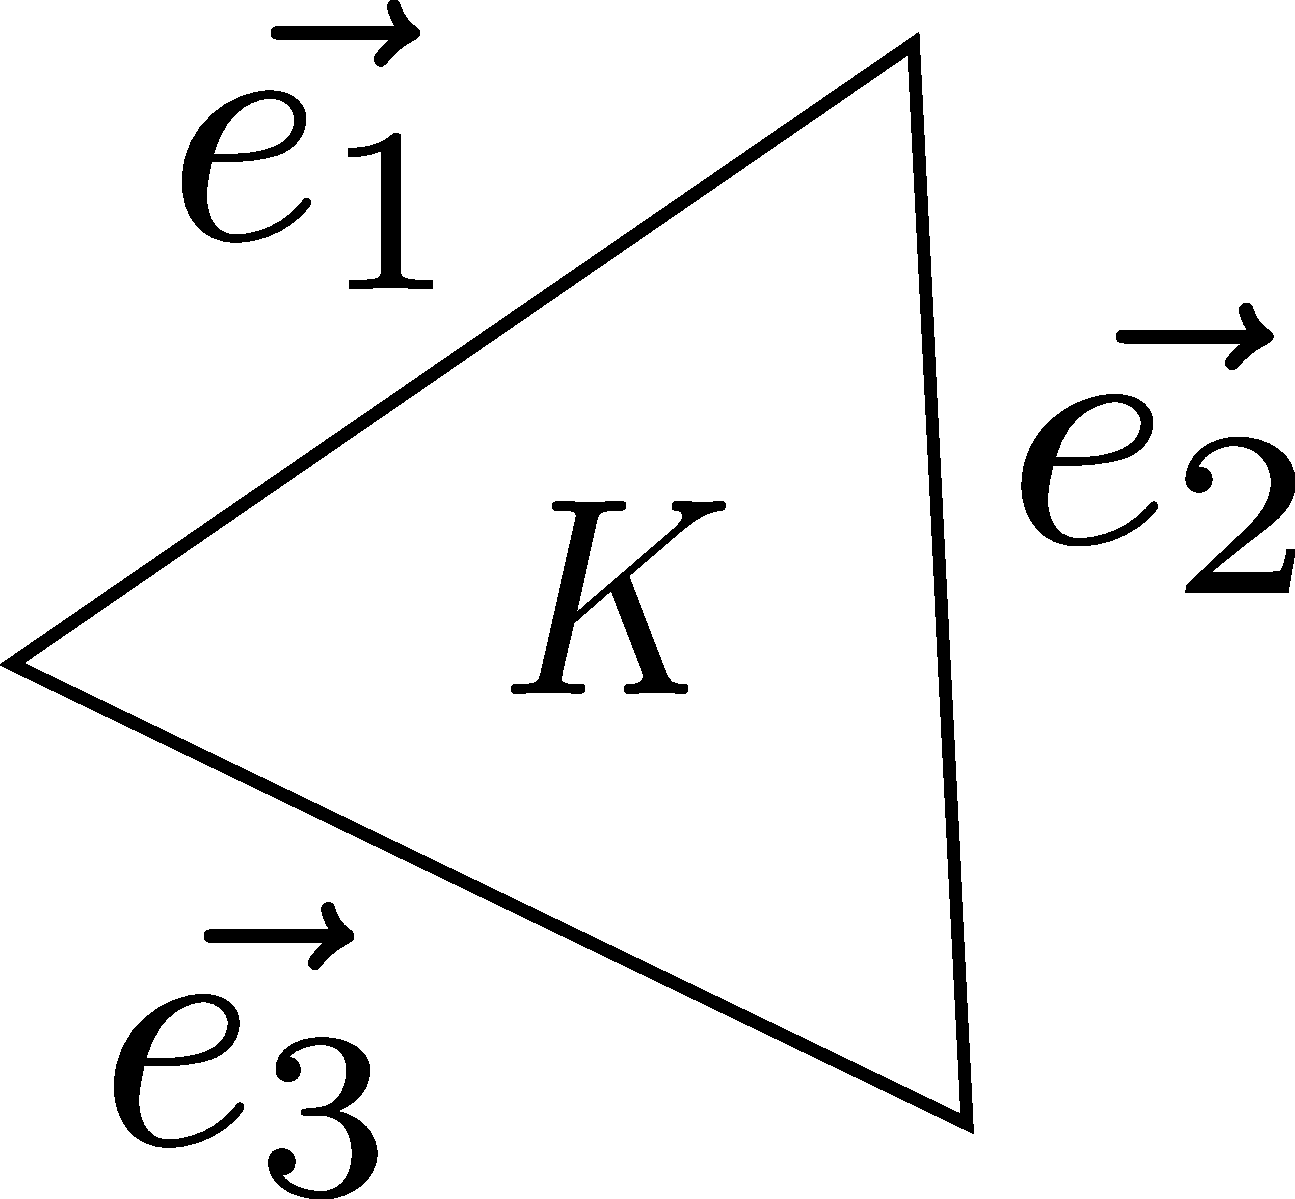
\includegraphics[scale=0.07]{image/triangle_error_frey}
%    \caption{Element $K$}
    \end{figure}
  \end{multicols}

  \uncover<2->{
  \vspace{-0.8cm}
  \begin{block}{Objective:}
    Adapt $\Triangles$ into $\Triangles$' such that:

    \begin{empheq}{align}
      \varepsilon &= \langle \overrightarrow{e}, \bar{\metric}(\element) \overrightarrow{e} \rangle \,, \qquad \forall \element \in \Triangles'\,, \qquad \forall \overrightarrow{e} \in E_\element. \\
            & \qquad \qquad \qquad \text{with:  } \metric = \frac{1}{\varepsilon} \bar{\metric}. \\
      1 &= \langle \overrightarrow{e}, \metric(\element) \overrightarrow{e} \rangle \,, \qquad \forall \element \in \Triangles'\,, \qquad \forall \overrightarrow{e} \in E_\element.
    \end{empheq}
  \end{block}
}

  \end{frame}



% ============================================
% ====== Frame : Algorithm principle    ======
% ============================================

%\setbeamercovered{transparent}
\begin{frame}{Mesh adaptation Algorithm}

  \begin{block}{Distance between $P$ and $M$ according to the metric field $\metric$:}
  \begin{empheq}{align}
\parallel \overrightarrow{PM} \parallel_\metric =  \int_{0}^{1} \sqrt{ \overrightarrow{PM}^\top  \metric( (1-t)P + tM) \overrightarrow{PM}  } \, dt \,.
  \end{empheq}
  \end{block}

  \begin{enumerate}
    \uncover<2->{
\item Scan all the edges $\overrightarrow{PM}$ and verify $\parallel \overrightarrow{PM} \parallel_\metric=1$:
\begin{itemize}
\item{Split the current edge if too long;}
\item{Collapse the edge if too short.}
\end{itemize}
    }
    \uncover<3->{
\item Check quality of the elements:
\begin{itemize}
\item Swap edges if "too bad elements";
\item{Move points.}
\end{itemize}
    }
    \uncover<3-4>{
\begin{tikzpicture}[remember picture,overlay]
    \node[xshift=80mm,yshift=-56mm,anchor=north west] at (current page.north west){%
    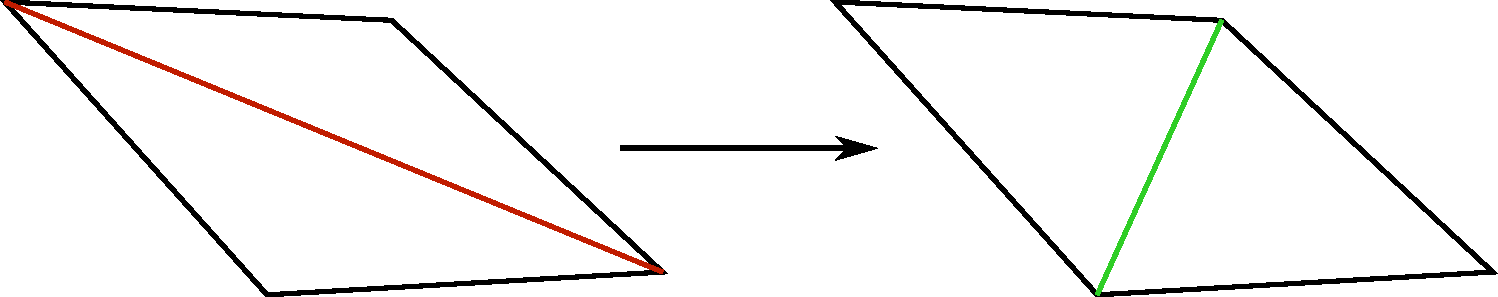
\includegraphics[width=40mm]{image/swap_edge.pdf}};
\end{tikzpicture}
}
    \uncover<4->{
      \vspace{-0.5cm}
    \item Go to 1. until convergence of the algorithm:
      \begin{empheq}{align}
        \frac{\sqrt{2}}{2} \le \parallel \overrightarrow{PM} \parallel_\metric \le \sqrt{2}\,.
      \end{empheq}
      }
\end{enumerate}

\end{frame}

%% %% \begin{frame}
%% %%   \begin{block}{Definition of Isotropic/ Anisotropic cells}
%% %% \begin{multicols}{2}
%% %%   \begin{figure}[H]
%% %% 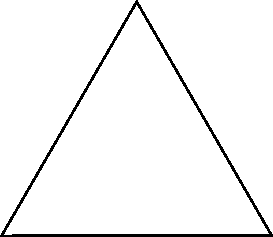
\includegraphics[scale=0.6]{image/isotropic_cell.pdf}
%% %% \caption{Isotropic cell  ($\lambda_1 = \lambda_2$).}
%% %% \end{figure}
%% %% \columnbreak
%% %% \begin{figure}
%% %% 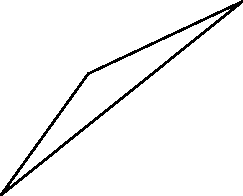
\includegraphics[scale=0.7]{image/anisotropic_cell.pdf}
%% %% \caption{Anisotropic cell ($\lambda_1 >> \lambda_2$).}
%% %% \end{figure}
%% %% \end{multicols}
%% %% \end{block}
%% %% \end{frame}




% ============================================
% ====== Frame : How to define the metric  ===
% ============================================
\subsection{Adaptation according to the physical parameters}
\begin{frame}{Define a metric according to the physical parameters}
  How to define a metric according to $\smodel^i$ instead of $S^i$ ?
  \vspace{0.5cm}
  \begin{multicols}{2}
    \vspace{-1cm}
    \begin{figure}
      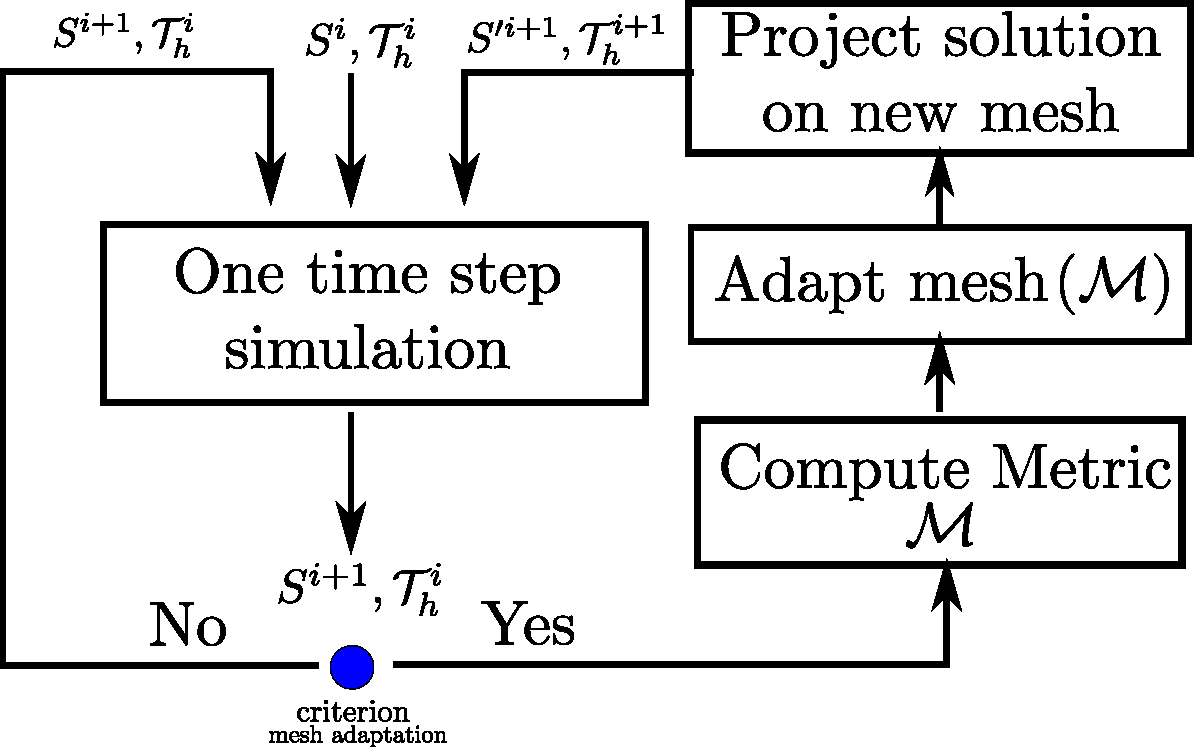
\includegraphics[scale=0.27]{image/mesh_adapt_workflow.pdf}
    \end{figure}
    \columnbreak
        \begin{figure}
      \includegraphics[scale=0.27]{image/mesh_adapt_workflow_fwi.pdf}
    \end{figure}
     \end{multicols}
\end{frame}


\begin{frame}[noframenumbering]{Define a metric according to the model parameters}
  \small
  No predominant directions $\longrightarrow$ Isotropic metric ($\metric(x) \approx h(x)$)

  \uncover<2->{
  In a reference square of size $\lambda \times \lambda$:
  \begin{empheq}{align}
    \nppw^2  &= \frac{\lambda^2}{a} \frac{(\PolOrder + 1)(\PolOrder + 2)}{2}, \text{  where: } \lambda = \velocity / \fmax
  \end{empheq}
  }

  \uncover<3->{
  Isotropic cell hypothesis:
  \begin{empheq}{align}
    a = \frac{\sqrt{3}}{4} h^2
  \end{empheq}
  }

  \uncover<4->{
  \begin{block}{Heuristic size map formula:}
  \begin{empheq}{align}
  \forall x \in \Domain, \, \,  h(x)=2\frac{\lambda(x)}{\nppw}\sqrt{\frac{(\PolOrder+1)(\PolOrder+2)}{2\sqrt{3}}} \,.
  \end{empheq}
  \end{block}
  }
\end{frame}




% ============================================
% ====== Frame : Find NPPW  ==================
% ============================================

\begin{frame}{Numerical assessement of the isotropic size map}{Determine the $\nppw$ value}
  \begin{multicols}{2}
    \begin{itemize}
    \item 2s simulation
    \item 1 source: First order ricker $\fpeak=10$Hz
    \item 462 receivers
    \item Constant velocity model (to avoid errors from mis-representation of the model)
    \item compare numerical traces with analytic traces \footcite{gar6more}
    \item for various $\nppw$ values
    \end{itemize}
    \columnbreak
  \begin{figure}[H]
  \centering
  \includegraphics[scale=0.31]{image/precision_test.pdf}
  \caption{Experimental setup for the accuracy assessment.}
  \label{homogeneous_prec}
  \end{figure}
  \end{multicols}
  \end{frame}


% ============================================
% ====== Frame : Graph error / nppw  =========
% ============================================

\begin{frame}{Error as a function of $\nppw$}
  \begin{figure}[H]
 \vspace{-0.3cm}
\centering
 \setlength{\plotwidth}{10cm}
    \setlength{\plotheight}{6.0cm}
    \begin{tikzpicture}
      \begin{axis}[%
          width=\plotwidth, height=\plotheight,,
          at={(0,0)},scale only axis,separate axis lines,
          ymode=log,
          xlabel={$\nppw$},
          ylabel={error},
          grid=both,
          grid style={line width=.1pt, draw=gray!10},
          major grid style={line width=.2pt,draw=gray!50},
          %%   ymode=log,
          %yminorticks=true,
          %% xmin=0,xmax=35,
          %% ymin=0,ymax=1.25,
          legend pos=north east
          %ymin=0.98,ymax=1.22
        ]

        %% load current data
        %% -----------------
        \addplot[color=blue!50!black,mark options={solid}, mark=triangle*,
          line width=1pt,
          mark size=2pt]
        table[x=ppw,y=error]
        {graph/mesh_error2.txt};
        \addlegendentry{P2}

 \addplot[color=red!50!black,mark options={solid}, mark=*,
          line width=1pt,
          mark size=2pt]
        table[x=ppw,y=error]
        {graph/mesh_error3.txt};
        \addlegendentry{P3}

 \addplot[color=green!50!black,mark options={solid}, mark=square*,
          line width=1pt,
          mark size=2pt]
        table[x=ppw,y=error]
        {graph/mesh_error4.txt};
        \addlegendentry{P4}

 \addplot[color=yellow!50!black,mark options={solid}, mark=diamond*,
          line width=1pt,
          mark size=2pt]
        table[x=ppw,y=error]
        {graph/mesh_error5.txt};
        \addlegendentry{P5}
      \end{axis}
      \uncover<2->{
       \draw [red,ultra thick,rounded corners] (0.0,0.67) -- (10,0.67);}
      %% --------------------------------------------------------------------
    \end{tikzpicture}
    \end{figure}
\end{frame}


%% \begin{frame}{Error as a function of the ratio $\lambda/h$}
%%   \begin{figure}[H]
%%     \vspace{-0.3cm}
%% \centering
%%  \setlength{\plotwidth}{10cm}
%%     \setlength{\plotheight}{6.0cm}
%%         \begin{tikzpicture}
%%       \begin{axis}[%
%%           width=\plotwidth, height=\plotheight,,
%%           at={(0,0)},scale only axis,separate axis lines,
%%           ymode=log,
%%           xlabel={$\lambda/h$},
%%           grid=both,
%%           grid style={line width=.1pt, draw=gray!10},
%%           major grid style={line width=.2pt,draw=gray!50},
%%           %%   ymode=log,
%%           %yminorticks=true,
%%           %% xmin=0,xmax=35,
%%           %% ymin=0,ymax=1.25,
%%           legend pos=north east
%%           %ymin=0.98,ymax=1.22
%%         ]

%%         %% load current data
%%         %% -----------------
%%         \addplot[color=blue!50!black,mark options={solid}, mark=triangle*,
%%           line width=1pt,
%%           mark size=2pt]
%%         table[x=ratio,y=error]
%%         {graph/mesh_error2.txt};
%%         \addlegendentry{P2}

%%  \addplot[color=red!50!black,mark options={solid}, mark=*,
%%           line width=1pt,
%%           mark size=2pt]
%%         table[x=ratio,y=error]
%%         {graph/mesh_error3.txt};
%%         \addlegendentry{P3}

%%  \addplot[color=green!50!black,mark options={solid}, mark=square*,
%%           line width=1pt,
%%           mark size=2pt]
%%         table[x=ratio,y=error]
%%         {graph/mesh_error4.txt};
%%         \addlegendentry{P4}

%%  \addplot[color=yellow!50!black,mark options={solid}, mark=diamond*,
%%           line width=1pt,
%%           mark size=2pt]
%%         table[x=ratio,y=error]
%%         {graph/mesh_error5.txt};
%%         \addlegendentry{P5}
%%       \end{axis}
%%       %% --------------------------------------------------------------------
%%       \uncover<2->{
%%       \draw [red,ultra thick,rounded corners] (0.0,0.67) -- (10,0.67);}
%%     \end{tikzpicture}
%%     \end{figure}
%% \end{frame}




% ============================================
% ====== Frame : Tableau recaptiulatif  ======
% ============================================

\begin{frame}{Summary of the experimental criterion}
  \small
      \hspace{-1cm}
  \begin{table}[!htbp]
    \begin{tabular}{|l|c|c|c|c|c|}
    \hline
        \textbf{Polynomial order ($\PolOrder$)} & 2 & 3 & 4 & 5 & 6 \\ \hline
        $\boldsymbol{\nppw}$  & 13 & 10 & 10 & 9 & 9 \\ \hline
        \textbf{Ratio} $\boldsymbol{\lambda/h}$ & 3.49 & 2.08 & 1.70 & 1.29 & 1.12 \\ \hline
        \textbf{Number of Element} & 303283 & 105788 & 69813 & 40012 & 29894 \\ \hline
        \textbf{Computational time (s)} & 5230 & 2764 & 1956 & 2017  & 1789\\ \hline
    \end{tabular}
    \caption{Summary table for 1$\%$ relative error for 2D DG acoustic solver on triangular grid.}
    \label{recap_ppw}
  \end{table}
  \uncover<2->{
  \begin{tikzpicture}[remember picture,overlay]
    \draw [red,ultra thick,rounded corners] (-1.6,2.1) rectangle (6.0,2.7);
%    \node[xshift=80mm,yshift=-56mm,anchor=north west] at (current page.north west){%
%    \includegraphics[width=40mm]{image/swap_edge.pdf}};
  \end{tikzpicture}
  }
\end{frame}







% ============================================
% ====== Frame : Validation   ================
% ============================================
\subsection{Validation of the isotropic metric}
\begin{frame}{Validation of the isotropic size map}
  \begin{block}{}
    Polynomial order fixed ($\PolOrder$) $\longrightarrow$ define mesh ($h$-adaptivity)
  \end{block}

  $\Updownarrow$

    \begin{block}{}
    Mesh given ($h$) $\longrightarrow$ define the polynomial order ($p$-adaptivity)
    \end{block}

    \uncover<2->{
      \vspace{-0.4cm}
\setlength{\modelwidth}{6.5cm}
\begin{figure}[!htbp]
  \renewcommand{\modelfile}{image/iso22_mesh}
     \begin{subfigure}[!htbp]{0.5\textwidth}
        \vspace{0.4cm}
        \hspace{-0.5cm}
         \centering
         \begin{tikzpicture}
\pgfmathsetmacro{\xmin} {0.}
\pgfmathsetmacro{\xmax} {9.7}
\pgfmathsetmacro{\zmin} {0.}
\pgfmathsetmacro{\zmax} {2.7}
\pgfmathsetmacro{\zzmax} {3.0}
\pgfmathsetmacro{\xxmax} {10.0}

\begin{axis}[%
width=1.0\modelwidth,
height=0.5\modelwidth,
axis on top, separate axis lines,
xmin=\xmin, xmax=\xxmax, %xlabel={x (km)},
ymin=\zmin, ymax=\zzmax,
yticklabels={},xticklabels={},
y dir=reverse,
point meta min=1.5e3, point meta max=4.6e3,
colorbar/width=2.5mm,
axis x line=top,thick,
axis y line=left,thick,
ylabel style={rotate=-90},
ylabel={$z$},
xlabel={$x$},
ticks = none,
]
\addplot [forget plot] graphics [xmin=\xmin,xmax=\xmax,ymin=\zmin,ymax=\zmax] {{\modelfile}.png};
\end{axis}
\end{tikzpicture}%

         \caption{Marmousi refined mesh at the interfaces (12809 elements).}
         \label{marmousi_mesh_padapt}
     \end{subfigure}
     \hspace{-1cm}
     \renewcommand{\modelfile}{image/iso22_order}
     \renewcommand{\cmapmin}{2}
     \renewcommand{\cmapmax}{4}
     \begin{subfigure}[!htbp]{0.5\textwidth}
        \vspace{-0.3cm}
         \centering
         \begin{tikzpicture}

\pgfmathsetmacro{\xmin} {0.}
\pgfmathsetmacro{\xmax} {9.7}
\pgfmathsetmacro{\zmin} {0.}
\pgfmathsetmacro{\zmax} {2.7}
\pgfmathsetmacro{\zzmax} {3.0}
\pgfmathsetmacro{\xxmax} {10.0}


\begin{axis}[%
width=1.0\modelwidth,
height=0.5\modelwidth,
axis on top, separate axis lines,
xmin=\xmin, xmax=\xxmax, %xlabel={x (km)},
ymin=\zmin, ymax=\zzmax,
yticklabels={},xticklabels={},
y dir=reverse,
colormap/jet, colorbar,
colorbar style={title=\small{order}},
point meta min=\cmapmin, point meta max=\cmapmax,
colorbar/width=2.5mm,
axis x line=top,thick,
axis y line=left,thick,
ylabel style={rotate=-90},
ylabel={$z$},
xlabel={$x$},
ticks = none,
]
\addplot [forget plot] graphics [xmin=\xmin,xmax=\xmax,ymin=\zmin,ymax=\zmax] {{\modelfile}.png};
\end{axis}
\end{tikzpicture}%

         \vspace{-0.9cm}
         \caption{$p$-adaptivity map.}
         \label{marmousi_order_padapt}
     \end{subfigure}

  \begin{tikzpicture}[remember picture,overlay]
    \draw [red,ultra thick,rounded corners, line width=0.1cm] (-6.2,3.45) rectangle (6.3,4.35);
%    \node[xshift=80mm,yshift=-56mm,anchor=north west] at (current page.north west){%
%    \includegraphics[width=40mm]{image/swap_edge.pdf}};
  \end{tikzpicture}
\end{figure}
     }
     \uncover<3->{
\vspace{-0.5cm}
\begin{table}[!htbp]
  \small
    \centering
    \begin{tabular}{|c|c|c|c|}
    \hline
         $p$-adaptivity    &  P2   & P3   &  P4   \\ \hline
        Number of elements & 1424  & 7981 & 3404   \\ \hline
        Pourcentage        & 11\%  &  63\%&  27\%  \\ \hline
    \end{tabular}
\end{table}
}
\end{frame}


\begin{frame}[noframenumbering]{Validation of the isotropic size map}
  \begin{block}{}
    Polynomial order fixed ($\PolOrder$) $\longrightarrow$ define mesh ($h$-adaptivity)
  \end{block}

  $\Updownarrow$

    \begin{block}{}
    Mesh given ($h$) $\longrightarrow$ define the polynomial order ($p$-adaptivity)
    \end{block}

      \vspace{-0.4cm}
\setlength{\modelwidth}{6.5cm}
\begin{figure}[!htbp]
  \renewcommand{\modelfile}{image/iso22_mesh}
     \begin{subfigure}[!htbp]{0.5\textwidth}
        \vspace{0.4cm}
        \hspace{-0.5cm}
         \centering
         \begin{tikzpicture}
\pgfmathsetmacro{\xmin} {0.}
\pgfmathsetmacro{\xmax} {9.7}
\pgfmathsetmacro{\zmin} {0.}
\pgfmathsetmacro{\zmax} {2.7}
\pgfmathsetmacro{\zzmax} {3.0}
\pgfmathsetmacro{\xxmax} {10.0}

\begin{axis}[%
width=1.0\modelwidth,
height=0.5\modelwidth,
axis on top, separate axis lines,
xmin=\xmin, xmax=\xxmax, %xlabel={x (km)},
ymin=\zmin, ymax=\zzmax,
yticklabels={},xticklabels={},
y dir=reverse,
point meta min=1.5e3, point meta max=4.6e3,
colorbar/width=2.5mm,
axis x line=top,thick,
axis y line=left,thick,
ylabel style={rotate=-90},
ylabel={$z$},
xlabel={$x$},
ticks = none,
]
\addplot [forget plot] graphics [xmin=\xmin,xmax=\xmax,ymin=\zmin,ymax=\zmax] {{\modelfile}.png};
\end{axis}
\end{tikzpicture}%

         \caption{Marmousi refined mesh at the interfaces (12809 elements).}
         \label{marmousi_mesh_padapt}
     \end{subfigure}
     \hspace{-1cm}
     \renewcommand{\modelfile}{image/iso22_order}
     \renewcommand{\cmapmin}{2}
     \renewcommand{\cmapmax}{4}
     \begin{subfigure}[!htbp]{0.5\textwidth}
        \vspace{-0.3cm}
         \centering
         \begin{tikzpicture}

\pgfmathsetmacro{\xmin} {0.}
\pgfmathsetmacro{\xmax} {9.7}
\pgfmathsetmacro{\zmin} {0.}
\pgfmathsetmacro{\zmax} {2.7}
\pgfmathsetmacro{\zzmax} {3.0}
\pgfmathsetmacro{\xxmax} {10.0}


\begin{axis}[%
width=1.0\modelwidth,
height=0.5\modelwidth,
axis on top, separate axis lines,
xmin=\xmin, xmax=\xxmax, %xlabel={x (km)},
ymin=\zmin, ymax=\zzmax,
yticklabels={},xticklabels={},
y dir=reverse,
colormap/jet, colorbar,
colorbar style={title=\small{order}},
point meta min=\cmapmin, point meta max=\cmapmax,
colorbar/width=2.5mm,
axis x line=top,thick,
axis y line=left,thick,
ylabel style={rotate=-90},
ylabel={$z$},
xlabel={$x$},
ticks = none,
]
\addplot [forget plot] graphics [xmin=\xmin,xmax=\xmax,ymin=\zmin,ymax=\zmax] {{\modelfile}.png};
\end{axis}
\end{tikzpicture}%

         \vspace{-0.9cm}
         \caption{$p$-adaptivity map.}
         \label{marmousi_order_padapt}
     \end{subfigure}

  \begin{tikzpicture}[remember picture,overlay]
    \draw [red,ultra thick,rounded corners, line width=0.1cm] (-6.3,3.45) rectangle (6.3,4.35);
%    \node[xshift=80mm,yshift=-56mm,anchor=north west] at (current page.north west){%
%    \includegraphics[width=40mm]{image/swap_edge.pdf}};
  \end{tikzpicture}
\end{figure}

\vspace{-0.5cm}
\begin{table}[!htbp]
  \small
    \centering
    \begin{tabular}{|c|c|c|c|c|c|}
    \hline
         & $p$-adaptivity & Full P2 & Full P3 & Full P4 & Full P5 \\ \hline
        L2 relative error & \cellcolor{green!30}0.38\%  & \cellcolor{red!30} 17.40\% & \cellcolor{red!30} 1.44\% & \cellcolor{green!30} 0.30\% &  ref. \\ \hline
        CPU Time (s) & \cellcolor{green!30} 815 & 502 & 1122 & \cellcolor{red!30}2244 & 3455 \\ \hline
    \end{tabular}
\end{table}
\end{frame}



% ============================================
% ====== Frame : Mesh refinement  ============
% ============================================
\subsection{Mesh refinement}
\begin{frame}{Interface refinement}{The metric, a flexible way to define the mesh}
 \small

\begin{overprint}
      \onslide<1>
      \begin{figure}[!htbp]
\centering
\includegraphics[scale=0.25]{image/grad_e.png}
\caption{Interface detection.}
\label{mesh_marmousi}
\end{figure}
      \onslide<2>
\begin{figure}[!htbp]
\centering
\includegraphics[scale=0.27]{image/marmousi_mesh.png}
\caption{Example of adapted meshes obtained with respect to a size map and taking into account sharp interfaces (42K elements).}
\label{mesh_marmousi}
\end{figure}
    \end{overprint}
\end{frame}




% ============================================
% ====== Frame :  Flowchart into fwi  ========
% ============================================

\subsection{Application to the FWI workflow}
\begin{frame}{Flowchart of remeshing process the FWI course.}

  \begin{figure}[htbp!]
    \vspace{-0.7cm}
  \centering
  \includegraphics[scale=0.36]{image/remesh_workflow0.pdf}
  \label{flowchart_remesh}
\end{figure}
\end{frame}

\begin{frame}[noframenumbering]{Flowchart of remeshing process the FWI course.}

  \begin{figure}[htbp!]
    \vspace{-0.7cm}
  \centering
  \includegraphics[scale=0.36]{image/remesh_workflow1.pdf}
  \label{flowchart_remesh}
\end{figure}
\end{frame}


\begin{frame}[noframenumbering]{Flowchart of remeshing process the FWI course.}

  \begin{figure}[htbp!]
    \vspace{-0.7cm}
  \centering
  \includegraphics[scale=0.36]{image/remesh_workflow2.pdf}
  \label{flowchart_remesh}
\end{figure}
\end{frame}


\begin{frame}[noframenumbering]{Flowchart of remeshing process the FWI course.}

  \begin{figure}[htbp!]
    \vspace{-0.7cm}
  \centering
  \includegraphics[scale=0.36]{image/remesh_workflow.pdf}
  \label{flowchart_remesh}
\end{figure}
\end{frame}




============================================
====== Frame :  Marmousi constant model ====
============================================

\begin{frame}{Comparaison with Marmousi model}{Constant with constant model per element}
    \vspace{-0.8cm}
  \setlength{\modelwidth}{6.0cm}
  \begin{figure}[!htbp]
    \renewcommand{\modelfile}{image/mesh_adapt/adapt_vp_80}
     \begin{subfigure}[!htbp]{0.5\textwidth}
        \vspace{0.5cm}
        \hspace{-0.5cm}
         \centering
         \begin{tikzpicture}
\pgfmathsetmacro{\xmin} {0.}
\pgfmathsetmacro{\xmax} {9.7}
\pgfmathsetmacro{\zmin} {0.}
\pgfmathsetmacro{\zmax} {2.7}
\pgfmathsetmacro{\zzmax} {3.0}
\pgfmathsetmacro{\xxmax} {10.0}

\begin{axis}[%
width=1.0\modelwidth,
height=0.5\modelwidth,
axis on top, separate axis lines,
xmin=\xmin, xmax=\xxmax, %xlabel={x (km)},
ymin=\zmin, ymax=\zzmax,
yticklabels={},xticklabels={},
y dir=reverse,
point meta min=1.5e3, point meta max=4.6e3,
colorbar/width=2.5mm,
axis x line=top,thick,
axis y line=left,thick,
ylabel style={rotate=-90},
ylabel={$z$},
xlabel={$x$},
ticks = none,
]
\addplot [forget plot] graphics [xmin=\xmin,xmax=\xmax,ymin=\zmin,ymax=\zmax] {{\modelfile}.png};
\end{axis}
\end{tikzpicture}%

         \caption*{Final model \textcolor{\mygreen}{\textbf{with mesh adaptation}}.}
         \label{marmousi_mesh_padapt}
     \end{subfigure}
     \hspace{-1cm}
     \renewcommand{\modelfile}{image/mesh_adapt/classic_vp_80}
     \renewcommand{\cmapmin}{1500}
     \renewcommand{\cmapmax}{5000}
     \begin{subfigure}[!htbp]{0.5\textwidth}
         \centering
         \begin{tikzpicture}
\pgfmathsetmacro{\xmin} {0.}
\pgfmathsetmacro{\xmax} {9.7}
\pgfmathsetmacro{\zmin} {0.}
\pgfmathsetmacro{\zmax} {2.7}
\pgfmathsetmacro{\zzmax} {3.0}
\pgfmathsetmacro{\xxmax} {10.0}


\begin{axis}[%
width=1.0\modelwidth,
height=0.5\modelwidth,
axis on top, separate axis lines,
xmin=\xmin, xmax=\xxmax, %xlabel={x (km)},
ymin=\zmin, ymax=\zzmax,
yticklabels={},xticklabels={},
y dir=reverse,
colormap/paraview, colorbar,
colorbar style={title=\small{$m \cdot s^{-1}$}},
point meta min=\cmapmin, point meta max=\cmapmax,
colorbar/width=2.5mm,
axis x line=top,thick,
axis y line=left,thick,
ylabel style={rotate=-90},
ylabel={$z$},
xlabel={$x$},
ticks = none,
]
\addplot [forget plot] graphics [xmin=\xmin,xmax=\xmax,ymin=\zmin,ymax=\zmax] {{\modelfile}.png};
\end{axis}
\end{tikzpicture}%

         \vspace{-0.6cm}
         \caption*{Final model \textcolor{blue}{\textbf{without mesh adaptation}}.}
     \end{subfigure}
       \end{figure}

  \uncover<2->{
    \scriptsize
\begin{table}[!htbp]
\centering
\begin{tabular}{|l|l|l|l|l|l|}
\hline
& 0-2Hz & 0-5Hz & 0-8Hz & 0-12Hz & 0-15Hz  \\ \hline
\rowcolor{green!30}
Number of elements   & 277    & 779     & 2090    & 4859     & 7065  \\
\rowcolor{green!30}
(with mesh adaptation)      &     &      &     &      &   \\ \hline
\rowcolor{blue!30}
Number of elements      & 7218    & 7218     & 7218    & 7218     & 7218  \\
\rowcolor{blue!30}
(without mesh adaptation)      &     &      &     &      &   \\ \hline
\end{tabular}
\caption{Comparison of the number of elements in the mesh for each frequency band for both strategies.}
\label{nb_elem_mesh_adapt}
\end{table}
}
\end{frame}


\begin{frame}[noframenumbering]{Comparaison with Marmousi model}{Constant with constant model per element}
  \vspace{-0.8cm}
  \setlength{\modelwidth}{6.0cm}
  \begin{figure}[!htbp]
    \renewcommand{\modelfile}{image/mesh_adapt/adapt_vp_80}
     \begin{subfigure}[!htbp]{0.5\textwidth}
        \vspace{0.5cm}
        \hspace{-0.5cm}
         \centering
         \begin{tikzpicture}
\pgfmathsetmacro{\xmin} {0.}
\pgfmathsetmacro{\xmax} {9.7}
\pgfmathsetmacro{\zmin} {0.}
\pgfmathsetmacro{\zmax} {2.7}
\pgfmathsetmacro{\zzmax} {3.0}
\pgfmathsetmacro{\xxmax} {10.0}

\begin{axis}[%
width=1.0\modelwidth,
height=0.5\modelwidth,
axis on top, separate axis lines,
xmin=\xmin, xmax=\xxmax, %xlabel={x (km)},
ymin=\zmin, ymax=\zzmax,
yticklabels={},xticklabels={},
y dir=reverse,
point meta min=1.5e3, point meta max=4.6e3,
colorbar/width=2.5mm,
axis x line=top,thick,
axis y line=left,thick,
ylabel style={rotate=-90},
ylabel={$z$},
xlabel={$x$},
ticks = none,
]
\addplot [forget plot] graphics [xmin=\xmin,xmax=\xmax,ymin=\zmin,ymax=\zmax] {{\modelfile}.png};
\end{axis}
\end{tikzpicture}%

                  \caption*{Final model \textcolor{\mygreen}{\textbf{with mesh adaptation}}.}         \label{marmousi_mesh_padapt}
     \end{subfigure}
     \hspace{-1cm}
     \renewcommand{\modelfile}{image/mesh_adapt/classic_vp_80}
     \renewcommand{\cmapmin}{1500}
     \renewcommand{\cmapmax}{5000}
     \begin{subfigure}[!htbp]{0.5\textwidth}
         \centering
         \begin{tikzpicture}
\pgfmathsetmacro{\xmin} {0.}
\pgfmathsetmacro{\xmax} {9.7}
\pgfmathsetmacro{\zmin} {0.}
\pgfmathsetmacro{\zmax} {2.7}
\pgfmathsetmacro{\zzmax} {3.0}
\pgfmathsetmacro{\xxmax} {10.0}


\begin{axis}[%
width=1.0\modelwidth,
height=0.5\modelwidth,
axis on top, separate axis lines,
xmin=\xmin, xmax=\xxmax, %xlabel={x (km)},
ymin=\zmin, ymax=\zzmax,
yticklabels={},xticklabels={},
y dir=reverse,
colormap/paraview, colorbar,
colorbar style={title=\small{$m \cdot s^{-1}$}},
point meta min=\cmapmin, point meta max=\cmapmax,
colorbar/width=2.5mm,
axis x line=top,thick,
axis y line=left,thick,
ylabel style={rotate=-90},
ylabel={$z$},
xlabel={$x$},
ticks = none,
]
\addplot [forget plot] graphics [xmin=\xmin,xmax=\xmax,ymin=\zmin,ymax=\zmax] {{\modelfile}.png};
\end{axis}
\end{tikzpicture}%

         \vspace{-0.6cm}
         \caption*{Final model \textcolor{blue}{\textbf{without mesh adaptation}}.}
     \end{subfigure}
     \end{figure}

     \scriptsize
\begin{table}[!htbp]
\begin{tabular}{|m{3cm}|l|l|l|l|l|l|}
\hline
& 0-2Hz     & 0-5Hz     & 0-8Hz     & 0-12Hz    & 0-15Hz    & Total \\ \hline
\rowcolor{green!30}
CPU time (h)          & 3         & 11        & 60        & 230       & 408       & 712   \\
\rowcolor{green!30}
(with mesh adaptation)          &          &         &         &        &        &    \\ \hline
\rowcolor{blue!30}
CPU time (h)       & $\sim$432 & $\sim$432 & $\sim$432 & $\sim$432 & $\sim$432 & 2164  \\
\rowcolor{blue!30}
 (without mesh adaptation)       &  &  &  &  &  &   \\ \hline
CPU time ratio \newline (No mesh adapt/mesh adapt)  &  144.0   &    39.3    &   7.2     &    1.9    &   1.1     & \cellcolor{red!30} 3.0   \\ \hline
\end{tabular}
\caption{CPU time comparison between FWI with and without mesh adaptation.}
\label{cpu_tab_1}
\end{table}
\end{frame}



% ============================================
% ====== Frame :  Marmousi WADG model ========
% ============================================

\begin{frame}{Comparaison with Marmousi model}{With WADG parametrization}
  \vspace{-0.8cm}
  \setlength{\modelwidth}{6.0cm}
  \begin{figure}[!htbp]
    \renewcommand{\modelfile}{image/mesh_adapt/wadg_adapt_vp_80}
     \begin{subfigure}[!htbp]{0.5\textwidth}
        \vspace{0.5cm}
        \hspace{-0.5cm}
         \centering
         \begin{tikzpicture}
\pgfmathsetmacro{\xmin} {0.}
\pgfmathsetmacro{\xmax} {9.7}
\pgfmathsetmacro{\zmin} {0.}
\pgfmathsetmacro{\zmax} {2.7}
\pgfmathsetmacro{\zzmax} {3.0}
\pgfmathsetmacro{\xxmax} {10.0}

\begin{axis}[%
width=1.0\modelwidth,
height=0.5\modelwidth,
axis on top, separate axis lines,
xmin=\xmin, xmax=\xxmax, %xlabel={x (km)},
ymin=\zmin, ymax=\zzmax,
yticklabels={},xticklabels={},
y dir=reverse,
point meta min=1.5e3, point meta max=4.6e3,
colorbar/width=2.5mm,
axis x line=top,thick,
axis y line=left,thick,
ylabel style={rotate=-90},
ylabel={$z$},
xlabel={$x$},
ticks = none,
]
\addplot [forget plot] graphics [xmin=\xmin,xmax=\xmax,ymin=\zmin,ymax=\zmax] {{\modelfile}.png};
\end{axis}
\end{tikzpicture}%

         \caption*{Final model \textcolor{\mygreen}{\textbf{with mesh adaptation}}.}
         \label{marmousi_mesh_padapt}
     \end{subfigure}
     \hspace{-1cm}
     \renewcommand{\modelfile}{image/mesh_adapt/wadg_classic_vp_80}
     \renewcommand{\cmapmin}{1500}
     \renewcommand{\cmapmax}{5000}
     \begin{subfigure}[!htbp]{0.5\textwidth}
         \centering
         \begin{tikzpicture}
\pgfmathsetmacro{\xmin} {0.}
\pgfmathsetmacro{\xmax} {9.7}
\pgfmathsetmacro{\zmin} {0.}
\pgfmathsetmacro{\zmax} {2.7}
\pgfmathsetmacro{\zzmax} {3.0}
\pgfmathsetmacro{\xxmax} {10.0}


\begin{axis}[%
width=1.0\modelwidth,
height=0.5\modelwidth,
axis on top, separate axis lines,
xmin=\xmin, xmax=\xxmax, %xlabel={x (km)},
ymin=\zmin, ymax=\zzmax,
yticklabels={},xticklabels={},
y dir=reverse,
colormap/paraview, colorbar,
colorbar style={title=\small{$m \cdot s^{-1}$}},
point meta min=\cmapmin, point meta max=\cmapmax,
colorbar/width=2.5mm,
axis x line=top,thick,
axis y line=left,thick,
ylabel style={rotate=-90},
ylabel={$z$},
xlabel={$x$},
ticks = none,
]
\addplot [forget plot] graphics [xmin=\xmin,xmax=\xmax,ymin=\zmin,ymax=\zmax] {{\modelfile}.png};
\end{axis}
\end{tikzpicture}%

         \vspace{-0.6cm}
                  \caption*{Final model \textcolor{blue}{\textbf{without mesh adaptation}}.}
     \end{subfigure}
  \end{figure}

  \scriptsize
  \begin{table}[!htbp]
\centering
\begin{tabular}{|m{3.5cm}|l|l|l|l|l|}
\hline
& 0-2Hz & 0-5Hz & 0-8Hz & 0-12Hz & 0-15Hz  \\ \hline
\rowcolor{green!30}
Number of elements \newline (with mesh adaptation)      & 277    & 754     & 1958    & 4465     & 6905  \\ \hline
\rowcolor{green!30}
Number of parameters \newline (with mesh adaptation)      & 5263    & 14326     &  37202   & 54340     & 131195  \\ \hline
\rowcolor{blue!30}
Number of elements \newline (without mesh adaptation)      & 7218    & 7218     & 7218    & 7218     & 7218  \\ \hline
\rowcolor{blue!30}
Number of parameters \newline (without mesh adaptation)      & 137142    & 137142     & 137142    & 137142     & 137142  \\ \hline
\end{tabular}
\caption{Number of elements and parameters for each frequency band.}
\label{nb_elem_mesh_adapt_wadg}
\end{table}
\end{frame}


\begin{frame}[noframenumbering]{Comparaison with Marmousi model}{Constant with WADG}
    \vspace{-0.8cm}
  \setlength{\modelwidth}{6.0cm}
  \begin{figure}[!htbp]
    \renewcommand{\modelfile}{image/mesh_adapt/wadg_adapt_vp_80}
     \begin{subfigure}[!htbp]{0.5\textwidth}
        \vspace{0.5cm}
        \hspace{-0.5cm}
         \centering
         \begin{tikzpicture}
\pgfmathsetmacro{\xmin} {0.}
\pgfmathsetmacro{\xmax} {9.7}
\pgfmathsetmacro{\zmin} {0.}
\pgfmathsetmacro{\zmax} {2.7}
\pgfmathsetmacro{\zzmax} {3.0}
\pgfmathsetmacro{\xxmax} {10.0}

\begin{axis}[%
width=1.0\modelwidth,
height=0.5\modelwidth,
axis on top, separate axis lines,
xmin=\xmin, xmax=\xxmax, %xlabel={x (km)},
ymin=\zmin, ymax=\zzmax,
yticklabels={},xticklabels={},
y dir=reverse,
point meta min=1.5e3, point meta max=4.6e3,
colorbar/width=2.5mm,
axis x line=top,thick,
axis y line=left,thick,
ylabel style={rotate=-90},
ylabel={$z$},
xlabel={$x$},
ticks = none,
]
\addplot [forget plot] graphics [xmin=\xmin,xmax=\xmax,ymin=\zmin,ymax=\zmax] {{\modelfile}.png};
\end{axis}
\end{tikzpicture}%

                  \caption*{Final model \textcolor{\mygreen}{\textbf{with mesh adaptation}}.}
         \label{marmousi_mesh_padapt}
     \end{subfigure}
     \hspace{-1cm}
     \renewcommand{\modelfile}{image/mesh_adapt/wadg_classic_vp_80}
     \renewcommand{\cmapmin}{1500}
     \renewcommand{\cmapmax}{5000}
     \begin{subfigure}[!htbp]{0.5\textwidth}
         \centering
         \begin{tikzpicture}
\pgfmathsetmacro{\xmin} {0.}
\pgfmathsetmacro{\xmax} {9.7}
\pgfmathsetmacro{\zmin} {0.}
\pgfmathsetmacro{\zmax} {2.7}
\pgfmathsetmacro{\zzmax} {3.0}
\pgfmathsetmacro{\xxmax} {10.0}


\begin{axis}[%
width=1.0\modelwidth,
height=0.5\modelwidth,
axis on top, separate axis lines,
xmin=\xmin, xmax=\xxmax, %xlabel={x (km)},
ymin=\zmin, ymax=\zzmax,
yticklabels={},xticklabels={},
y dir=reverse,
colormap/paraview, colorbar,
colorbar style={title=\small{$m \cdot s^{-1}$}},
point meta min=\cmapmin, point meta max=\cmapmax,
colorbar/width=2.5mm,
axis x line=top,thick,
axis y line=left,thick,
ylabel style={rotate=-90},
ylabel={$z$},
xlabel={$x$},
ticks = none,
]
\addplot [forget plot] graphics [xmin=\xmin,xmax=\xmax,ymin=\zmin,ymax=\zmax] {{\modelfile}.png};
\end{axis}
\end{tikzpicture}%

         \vspace{-0.6cm}
                  \caption*{Final model \textcolor{blue}{\textbf{without mesh adaptation}}.}
     \end{subfigure}
  \end{figure}

  \scriptsize
\begin{table}[!htbp]
\begin{tabular}{|m{4.0cm}|l|l|l|l|l|l|}
\hline
& 0-2Hz     & 0-5Hz     & 0-8Hz     & 0-12Hz    & 0-15Hz    & Total  \\ \hline
\rowcolor{green!30}
CPU time (h)          & 5         & 22        & 73        & 334       & 541       & 975   \\
\rowcolor{green!30}
(with mesh adaptation)          &          &         &         &        &        &    \\ \hline
\rowcolor{blue!30}
CPU time (h)       & $\sim$730 & $\sim$730 & $\sim$730 & $\sim$730 & $\sim$730 & 3654   \\
\rowcolor{blue!30}
(without mesh adaptation)       &  &  &  &  &  &    \\ \hline
CPU time ratio \newline (without/with mesh adaptation) &  146.0    &    33.2   &   10.0    &    2.2    &   1.3     & \cellcolor{red!30} 3.75   \\ \hline
\end{tabular}
\caption{CPU time comparison between FWI with and without mesh adaptation.}
\label{wadg_cpu_tab}
\end{table}
\end{frame}




% ============================================
% ====== Frame :  Overthrust Mesh Adapt ======
% ============================================




\begin{frame}{Exploit all the DG properties to reconstruct Overthrust 2D model}
 \vspace{-0,8cm}
\setlength{\modelwidth}{6.0cm}
\begin{figure}[!htbp]
  \begin{subfigure}{0.5\textwidth}
    \vspace{0.5cm}
    \hspace{-0.5cm}
\renewcommand{\modelfile}{image/mesh_adapt/overthrust_ini}
\begin{tikzpicture}
  \pgfmathsetmacro{\xmin} {0.}
\pgfmathsetmacro{\xmax} {9.7}
\pgfmathsetmacro{\zmin} {0.}
\pgfmathsetmacro{\zmax} {2.7}
\pgfmathsetmacro{\zzmax} {3.0}
\pgfmathsetmacro{\xxmax} {10.0}

\begin{axis}[%
width=1.0\modelwidth,
height=0.5\modelwidth,
axis on top, separate axis lines,
xmin=\xmin, xmax=\xxmax, %xlabel={x (km)},
ymin=\zmin, ymax=\zzmax,
yticklabels={},xticklabels={},
y dir=reverse,
point meta min=1.5e3, point meta max=5.5e3,
axis x line=top,thick,
axis y line=left,thick,
ylabel style={rotate=-90},
ylabel={$z$},
xlabel={$x$},
ticks = none,
]
\addplot [forget plot] graphics [xmin=\xmin,xmax=\xmax,ymin=\zmin,ymax=\zmax] {{\modelfile}.png};
\end{axis}
\end{tikzpicture}%

\caption*{Blind wavespeed model.}
\label{target_model_2}
\end{subfigure}
\hspace{-1cm}
\begin{subfigure}{0.5\textwidth}
%\vspace{0.2cm}
\renewcommand{\modelfile}{image/mesh_adapt/overthrust}
\renewcommand{\cmapmin}{2500}
\renewcommand{\cmapmax}{5500}
\begin{tikzpicture}
\pgfmathsetmacro{\xmin} {0.}
\pgfmathsetmacro{\xmax} {9.7}
\pgfmathsetmacro{\zmin} {0.}
\pgfmathsetmacro{\zmax} {2.7}
\pgfmathsetmacro{\zzmax} {3.0}
\pgfmathsetmacro{\xxmax} {10.0}


\begin{axis}[%
width=1.0\modelwidth,
height=0.5\modelwidth,
axis on top, separate axis lines,
xmin=\xmin, xmax=\xxmax, %xlabel={x (km)},
ymin=\zmin, ymax=\zzmax,
yticklabels={},xticklabels={},
y dir=reverse,
colormap/paraview, colorbar,
colorbar style={title=\small{$m \cdot s^{-1}$}},
point meta min=\cmapmin, point meta max=\cmapmax,
colorbar/width=2.5mm,
axis x line=top,thick,
axis y line=left,thick,
ylabel style={rotate=-90},
ylabel={$z$},
xlabel={$x$},
ticks = none,
]
\addplot [forget plot] graphics [xmin=\xmin,xmax=\xmax,ymin=\zmin,ymax=\zmax] {{\modelfile}.png};
\end{axis}
\end{tikzpicture}%

\vspace{-0.6cm}
\caption*{Target wavespeed model.}
\label{blind_model_2}
\end{subfigure}
\label{overthrust_ini_and_blind}
\end{figure}

\begin{overprint}
  \onslide<2>
  \scriptsize
  \begin{table}[!htbp]
    \centering
    \begin{tabular}{|l|l|l|l|l|l|}
      \hline
      & 0-2Hz & 0-5Hz & 0-8Hz & 0-12Hz & 0-15Hz                               \\ \hline
      Number of elements $(\nbelem)$   & 391    & 907     &  5144   & 11252     & 1825               \\ \hline
      Number of parameters             & 7429   & 13605   &  36008  & 11252     & 51100              \\ \hline
      Polynomial order $(\PolOrder)$   & 4      & 3       &  2      & 2         & 5                  \\ \hline
      WADG quadrature order $(\QuadOrder)$   & 9      & 7       &  5      & 1         & 11           \\ \hline
      Polynomial basis   & Nodal      & Nodal       &  Nodal      & Nodal         & Bernstein-Bézier \\ \hline
    \end{tabular}
    \label{nb_elem_overthrust}
  \end{table}

  \onslide<3>

  \vspace{-1.0cm}
  \begin{block}{Animation of the reconstruction}
      \begin{center}
      \movie[showcontrols,loop,autostart]
            {\includegraphics[scale=.3]{animation/overthrust/overthrust_adapt-00.png}}
            {animation/overthrust/out.avi}
      \end{center}
    \end{block}

\end{overprint}

\end{frame}


\begin{frame}{Conclusion}
\end{frame}

\begin{frame}{Perspectives}
  \end{frame}
    %% Some results

 \printbibliography

%% \begin{frame}[noframenumbering]

\Large{\textbf{Appendices}}

\end{frame}


\begin{frame}[noframenumbering]

\Large{\textbf{Interface refinement}}

\end{frame}


\begin{frame}[noframenumbering]{Influence of the cloud point on the gradient}
\begin{figure}[H]
\centering
\includegraphics[scale=0.5]{image/histo_comparison_grad.pdf}
\caption{Histogram recording the number of points in the
point cloud as a function of the normalized gradient amplitude for two different point clouds.}
\label{histo_comparison_grad}
\end{figure}
\end{frame}



\begin{frame}[noframenumbering]{Influence of epsilon of the interface detection}
  \small
\setlength{\modelwidth}{6.1cm}
\begin{figure}[!htbp]
\renewcommand{\cmapmin}{0}
\renewcommand{\cmapmax}{1}
\renewcommand{\modelfile}{image/mesh_adapt/interface_tresh_02}
\begin{subfigure}{0.5\textwidth}
\vspace{0.0cm}
\centering
\begin{tikzpicture}
\pgfmathsetmacro{\xmin} {0.}
\pgfmathsetmacro{\xmax} {9.7}
\pgfmathsetmacro{\zmin} {0.}
\pgfmathsetmacro{\zmax} {2.7}
\pgfmathsetmacro{\zzmax} {3.0}
\pgfmathsetmacro{\xxmax} {10.0}

\begin{axis}[%
width=1.0\modelwidth,
height=0.5\modelwidth,
axis on top, separate axis lines,
xmin=\xmin, xmax=\xxmax, %xlabel={x (km)},
ymin=\zmin, ymax=\zzmax,
yticklabels={},xticklabels={},
y dir=reverse,
point meta min=1.5e3, point meta max=4.6e3,
colorbar/width=2.5mm,
axis x line=top,thick,
axis y line=left,thick,
ylabel style={rotate=-90},
ylabel={$z$},
xlabel={$x$},
ticks = none,
]
\addplot [forget plot] graphics [xmin=\xmin,xmax=\xmax,ymin=\zmin,ymax=\zmax] {{\modelfile}.png};
\end{axis}
\end{tikzpicture}%

\caption{Interfaces highlighted using $\epsilon=0.2$.}
\end{subfigure}
\hspace{-0.5cm}
\renewcommand{\modelfile}{image/mesh_adapt/interface_tresh_01}
\begin{subfigure}{0.5\textwidth}
\centering
\begin{tikzpicture}
\pgfmathsetmacro{\xmin} {0.}
\pgfmathsetmacro{\xmax} {9.7}
\pgfmathsetmacro{\zmin} {0.}
\pgfmathsetmacro{\zmax} {2.7}
\pgfmathsetmacro{\zzmax} {3.0}
\pgfmathsetmacro{\xxmax} {10.0}


\begin{axis}[%
    width=1.0\modelwidth,
    height=0.5\modelwidth,
    axis on top, separate axis lines,
    xmin=\xmin, xmax=\xxmax, %xlabel={x (km)},
    ymin=\zmin, ymax=\zzmax,
    yticklabels={},xticklabels={},
    y dir=reverse,
    colormap/jet, colorbar,
    point meta min=\cmapmin, point meta max=\cmapmax,
    colorbar/width=2.5mm,
    axis x line=top,thick,
    axis y line=left,thick,
    ylabel style={rotate=-90},
    ylabel={$z$},
    xlabel={$x$},
    ticks = none,
]
\addplot [forget plot] graphics [xmin=\xmin,xmax=\xmax,ymin=\zmin,ymax=\zmax] {{\modelfile}.png};
\end{axis}
\end{tikzpicture}%

\vspace{-0.7cm}
\caption{Interfaces highlighted using $\epsilon=0.1$.}
\end{subfigure}

\renewcommand{\modelfile}{image/grad_e}
\begin{subfigure}{0.5\textwidth}
\vspace{0.0cm}
\centering
\begin{tikzpicture}
\pgfmathsetmacro{\xmin} {0.}
\pgfmathsetmacro{\xmax} {9.7}
\pgfmathsetmacro{\zmin} {0.}
\pgfmathsetmacro{\zmax} {2.7}
\pgfmathsetmacro{\zzmax} {3.0}
\pgfmathsetmacro{\xxmax} {10.0}

\begin{axis}[%
width=1.0\modelwidth,
height=0.5\modelwidth,
axis on top, separate axis lines,
xmin=\xmin, xmax=\xxmax, %xlabel={x (km)},
ymin=\zmin, ymax=\zzmax,
yticklabels={},xticklabels={},
y dir=reverse,
point meta min=1.5e3, point meta max=4.6e3,
colorbar/width=2.5mm,
axis x line=top,thick,
axis y line=left,thick,
ylabel style={rotate=-90},
ylabel={$z$},
xlabel={$x$},
ticks = none,
]
\addplot [forget plot] graphics [xmin=\xmin,xmax=\xmax,ymin=\zmin,ymax=\zmax] {{\modelfile}.png};
\end{axis}
\end{tikzpicture}%

\caption{Interfaces highlighted using $\epsilon=0.08$.}
\end{subfigure}
\hspace{-0.5cm}
\begin{subfigure}{0.5\textwidth}
\centering
\renewcommand{\modelfile}{image/mesh_adapt/interface_tresh_002}
\begin{tikzpicture}
\pgfmathsetmacro{\xmin} {0.}
\pgfmathsetmacro{\xmax} {9.7}
\pgfmathsetmacro{\zmin} {0.}
\pgfmathsetmacro{\zmax} {2.7}
\pgfmathsetmacro{\zzmax} {3.0}
\pgfmathsetmacro{\xxmax} {10.0}


\begin{axis}[%
    width=1.0\modelwidth,
    height=0.5\modelwidth,
    axis on top, separate axis lines,
    xmin=\xmin, xmax=\xxmax, %xlabel={x (km)},
    ymin=\zmin, ymax=\zzmax,
    yticklabels={},xticklabels={},
    y dir=reverse,
    colormap/jet, colorbar,
    point meta min=\cmapmin, point meta max=\cmapmax,
    colorbar/width=2.5mm,
    axis x line=top,thick,
    axis y line=left,thick,
    ylabel style={rotate=-90},
    ylabel={$z$},
    xlabel={$x$},
    ticks = none,
]
\addplot [forget plot] graphics [xmin=\xmin,xmax=\xmax,ymin=\zmin,ymax=\zmax] {{\modelfile}.png};
\end{axis}
\end{tikzpicture}%

\vspace{-0.7cm}
\caption{Interfaces highlighted using $\epsilon=0.02$.}
\end{subfigure}
\caption{Marmousi highlighted interfaces for several threshold values.}
\label{interface_thresholds}
\end{figure}
\end{frame}


\begin{frame}[noframenumbering]{Modify the metric $\metric$ to deals with interface}
  if $Interface(P) = 1$

  \begin{multicols}{2}
    \large{\textbf{\textcolor{\mygreen}{Isotropic metric}}}
    \vspace{0.5cm}

    \uncover<2->{
    \small{In all direction:}
    \normalsize
    \begin{equation}
      \scriptstyle
      h(P) =  \frac{1}{r} 2\frac{\lambda(P)}{\nppw}\sqrt{\frac{(\PolOrder+1)(\PolOrder+2)}{2\sqrt{3}}},\, r\geq1.0
    \end{equation}
    \vfill
    }

    \columnbreak

    \large{\textbf{\textcolor{blue}{Anisotropic metric}}}
    \vspace{0.5cm}

    \uncover<3->{
    \small{In $\vec{\nabla} \velocity$ direction:}
    \normalsize
    \begin{equation}
      \scriptstyle
      hr(P) =  \frac{1}{r} 2\frac{\lambda(P)}{\nppw}\sqrt{\frac{(\PolOrder+1)(\PolOrder+2)}{2\sqrt{3}}},\, r\geq1.0
    \end{equation}

    \small{In $\vec{\nabla} \velocity^\top$ direction:}
    \normalsize
    \begin{equation}
      \scriptstyle
      h(P) =  2\frac{\lambda(P)}{\nppw}\sqrt{\frac{(\PolOrder+1)(\PolOrder+2)}{2\sqrt{3}}}.
    \end{equation}
    \vfill
    }

    \end{multicols}

\end{frame}


\begin{frame}[noframenumbering]

  \begin{multicols}{2}
    \large{\textbf{\textcolor{\mygreen}{Isotropic metric}}}

    \columnbreak

    \large{\textbf{\textcolor{blue}{Anisotropic metric}}}

  \end{multicols}

  \begin{table}[H]
    \small
\centering
\begin{tabular}{|l|l|l|l|l|l|l|l|}
\hline
& $\nbelem$  & $r$  & P2 & P3 & P4 &  CPU & Relative  \\
&  & &  &  &  & time(s) & L2 error \\ \hline
Mesh 1 &6808 &  1           &  <0.1\% & 8\% &92\% & 379 & 15.2\% \\ \hline
\rowcolor{green!30}
Mesh 2 &8434 &  $\sqrt{2}$  & 2\% & 25\% & 73\% & 463 & 10.5\% \\ \hline
\rowcolor{blue!30}
Mesh 2'&8226 &  $\sqrt{2}$  & 1\% & 14\% & 85\% & 602 & 8.5\% \\ \hline
\rowcolor{green!30}
Mesh 3 &12809&  2           & 24\% &62\% & 27\% & 815 & 5.2\% \\ \hline
\rowcolor{blue!30}
Mesh 3'&11496&  2           & 5\% & 37\% & 58\% & 1731 & 5.1\%  \\ \hline
Mesh 4 &26621&  ref.        & 0\% & 0\% & 100\% & 4384 & ref. \\ \hline
\end{tabular}
\caption{Performance comparison between isotropic and anisotropic mesh refinement.}
\label{mesh_iso_aniso_comp}
\end{table}
  \end{frame}



\begin{frame}[noframenumbering]{Modify the metric $\metric$ to deals with interface}


  \begin{multicols}{2}
        \large{\textbf{\textcolor{\mygreen}{Isotropic metric}}}
    \vspace{0.5cm}
    \begin{itemize}
      \item[\textcolor{\mygreen}{\textbf{+}}] Better capture the interfaces
      \item[\textcolor{\mygreen}{\textbf{+}}] Enhenced precision
      \item[\textcolor{\mygreen}{\textbf{+}}] Adapted for explicit time schemes
      \item[\textcolor{\myred}{\textbf{-}}] Have more $\dof$ for a lower accuracy
      \end{itemize}

    \columnbreak
    \large{\textbf{\textcolor{blue}{Anisotropic metric}}}
    \vspace{0.5cm}
    \begin{itemize}
      \item[\textcolor{\mygreen}{\textbf{+}}] Better capture the interfaces
      \item[\textcolor{\mygreen}{\textbf{++}}] Enhenced precision
      \item[\textcolor{\myred}{\textbf{- -}}] Not adapted for explicit time schemes
      \item[\textcolor{\mygreen}{\textbf{++}}] Get lower $\dof$ for a better accuracy
    \end{itemize}
  \end{multicols}

  \uncover<2->{
    \begin{block}{Warning}
      The refinement depends on the interface detection which is still an empirical selection ($\epsilon$).
    \end{block}
    }

\end{frame}



\end{document}
